\documentclass[a4paper,11pt]{article}
\usepackage[table]{xcolor}




\usepackage[T1]{fontenc}
\usepackage[normalem]{ulem}
\usepackage{mathtools}
\usepackage{blkarray,bigstrut} 
\usepackage{graphicx,wrapfig,lipsum}
\usepackage{tcolorbox}
\usepackage{enumitem}
\usepackage{array}
\usepackage{algorithm}
\usepackage{algorithmic}
\usepackage{mathpartir}
\usepackage{multirow}
\usepackage{hyperref}
\usepackage{amssymb}
\usepackage{subcaption}
\usepackage{stmaryrd}
\usepackage{color} 


\usepackage{tikz}
\usetikzlibrary{snakes}
\usetikzlibrary{svg.path} 
\usetikzlibrary{calc} 
\usetikzlibrary{shapes}
\usetikzlibrary{shapes.geometric}
\usetikzlibrary{arrows.meta}
\usetikzlibrary{arrows}
\usetikzlibrary{decorations.text,decorations.markings}
% % % % 

%%%%%%%%%%Packages for adaoption%%%

% \usepackage{amsthm} 

%Packages

%%%%%%%%%%%%%%%%%%%%%%%%%%%%%%%%%%%%%%%%%%%%%%%%%%%%%%%%%%%%%%%%%%%%%%%%%%%%%%%%%%%%%%%%%%%%%%%%%%%%%%%%%%%%%%%%%%%%%%%%%%%%%%%%%%%%%%%%%
%%%%%%%%%%%%%%%%%%%%%%%%%%%%%%%%%%%%%%%%%%%%%%%%%%%%% COMMANDS FOR GENERAL PAPER WRITING %%%%%%%%%%%%%%%%%%%%%%%%%%%%%%%%%%%%%%%%%%%%%%%%%%%%
%%%%%%%%%%%%%%%%%%%%%%%%%%%%%%%%%%%%%%%%%%%%%%%%%%%%%%%%%%%%%%%%%%%%%%%%%%%%%%%%%%%%%%%%%%%%%%%%%%%%%%%%%%%%%%%%%%%%%%%%%%%%%%%%%%%%%%%%%

%%%%%%%%%%%%%%%%%% LINK STYLE:
\hypersetup{
  colorlinks=true,
  linkcolor=blue!50!red,
  urlcolor=green!70!black
}

%%%%%%%%%%%%%%%%%%%%%%%%%%%% Theorem, Definition and Proof
\newtheorem{lem}{Lemma}[section]
\newtheorem{thm}{Theorem}[section]
\newtheorem{defn}{Definition}
\newtheorem{coro}{Corollary}[thm]

\newtheorem{example}{Example}[section]

\newcommand{\todo}[1]{{\color{red}\textbf{[[ #1 ]]}}}
\newcommand{\todomath}[1]{{\scriptstyle \color{red}\mathbf{[[ #1 ]]}}}
\newcommand{\completeness}[1]{{\color{blue}\textbf{[[ #1 ]]}}}
\newcommand{\caseL}[1]{\item \textbf{case: #1}\newline}
\newcommand{\subcaseL}[1]{\item \textbf{sub-case: #1}\newline}
\newcommand{\subsubcaseL}[1]{\item \textbf{subsub-case: #1}\newline}
\newcommand{\subsubsubcaseL}[1]{\item \textbf{subsubsub-case: \boldmath{#1}}\newline}

\newcommand{\blue}[1]{{\tiny \color{blue}{ #1 }}}


\let\originalleft\left
\let\originalright\right
\renewcommand{\left}{\mathopen{}\mathclose\bgroup\originalleft}
\renewcommand{\right}{\aftergroup\egroup\originalright}
\newcommand{\ts}[1]{ \llparenthesis {#1} \rrparenthesis }

\theoremstyle{definition}

\newtheorem{case}{Case}
\newtheorem{subcase}{Case}
\numberwithin{subcase}{case}
\newtheorem{subsubcase}{Case}
\numberwithin{subsubcase}{subcase}

\newtheorem{subsubsubcase}{Case}
\numberwithin{subsubsubcase}{subsubcase}
\newcommand{\st}{~.~}

%%%%COLORS
\definecolor{periwinkle}{rgb}{0.8, 0.8, 1.0}
\definecolor{powderblue}{rgb}{0.69, 0.88, 0.9}
\definecolor{sandstorm}{rgb}{0.93, 0.84, 0.25}
\definecolor{trueblue}{rgb}{0.0, 0.45, 0.81}

\newlength\Origarrayrulewidth
% horizontal rule equivalent to \cline but with 2pt width
\newcommand{\Cline}[1]{%
 \noalign{\global\setlength\Origarrayrulewidth{\arrayrulewidth}}%
 \noalign{\global\setlength\arrayrulewidth{2pt}}\cline{#1}%
 \noalign{\global\setlength\arrayrulewidth{\Origarrayrulewidth}}%
}

% draw a vertical rule of width 2pt on both sides of a cell
\newcommand\Thickvrule[1]{%
  \multicolumn{1}{!{\vrule width 2pt}c!{\vrule width 2pt}}{#1}%
}

% draw a vertical rule of width 2pt on the left side of a cell
\newcommand\Thickvrulel[1]{%
  \multicolumn{1}{!{\vrule width 2pt}c|}{#1}%
}

% draw a vertical rule of width 2pt on the right side of a cell
\newcommand\Thickvruler[1]{%
  \multicolumn{1}{|c!{\vrule width 2pt}}{#1}%
}

\newenvironment{subproof}[1][\proofname]{%
  \renewcommand{\qedsymbol}{$\blacksquare$}%
  \begin{proof}[#1]%
}{%
  \end{proof}%
}
%%%%%%%%%%%%%%%%%%%%%%%%%%%%%%% Fonts Definition %%%%%%%%%%%%%%%%%%%%%%%%%%%
\newcommand{\omitthis}[1]{}

% Misc.
\newcommand{\etal}{\textit{et al.}}
\newcommand{\bump}{\hspace{3.5pt}}

% Text fonts
\newcommand{\tbf}[1]{\textbf{#1}}

% Math fonts
\newcommand{\mbb}[1]{\mathbb{#1}}
\newcommand{\mbf}[1]{\mathbf{#1}}
\newcommand{\mrm}[1]{\mathrm{#1}}
\newcommand{\mtt}[1]{\mathtt{#1}}
\newcommand{\mcal}[1]{\mathcal{#1}}
\newcommand{\mfrak}[1]{\mathfrak{#1}}
\newcommand{\msf}[1]{\mathsf{#1}}
\newcommand{\mscr}[1]{\mathscr{#1}}

\newcommand{\diam}{{\color{red}\diamond}}
\newcommand{\dagg}{{\color{blue}\dagger}}
\let\oldstar\star
\renewcommand{\star}{\oldstar}

\newcommand{\im}[1]{\ensuremath{#1}}

\newcommand{\kw}[1]{\im{\mathtt{#1}}}
\newcommand{\set}[1]{\im{\{{#1}\}}}

\newcommand{\mmax}{\ensuremath{\mathsf{max}}}

\lstnewenvironment{ocaml}[2][]%
  {\lstset{language=ocaml,style=ocaml-pretty,captionpos=t,abovecaptionskip=-\medskipamount,caption={#2},#1}}
  %
  {}

\makeatletter
\newcommand{\mysmallishfont}{\@setfontsize\mysmallishfont{8.7pt}{9.7pt}}
\makeatother

\makeatletter
\newcommand{\myecfont}{\@setfontsize\myecfont{9.7pt}{10.7pt}}
\makeatother

\makeatletter
\newcommand{\myecsmfont}{\@setfontsize\myecfont{8.7pt}{9.7pt}}
\makeatother

\lstdefinelanguage{ocaml}{
  style=ocaml-default,
  keywordsprefix={'},
  morekeywords=[1]{},
  morekeywords=[2]{type,op,axiom,lemma,module,pred,const,declare},
  morekeywords=[3]{var,proc},
  morekeywords=[4]{while,if,then,else,elif,return,proof,qed,realize,rec, match},
}

\lstdefinestyle{ocaml-default}{
  escapechar=\#,
  upquote=true,
  columns=fullflexible,
  captionpos=b,
  frame=tb,
  xleftmargin=0pt,
  xrightmargin=0pt,
  rangebeginprefix={(**\ begin\ },
  rangeendprefix={(**\ end\ },
  rangesuffix={\ *)},
  includerangemarker=false,
  basicstyle=\mysmallishfont\sffamily,
  identifierstyle={},
  keywordstyle=[1]{\itshape},
  keywordstyle=[2]{\bfseries},
  keywordstyle=[3]{\bfseries},
  keywordstyle=[4]{\bfseries},
  keywordstyle=[5]{\bfseries},
  keywordstyle=[6]{\bfseries},
  keywordstyle=[7]{},
  keywordstyle=[8]{\bfseries},
  keywordstyle=[9]{\bfseries},
  literate={phi}{{$\!\phi\,$}}1
           {phi1}{{$\!\phi_1$}}1
           {phi2}{{$\!\phi_2$}}1
           {phi3}{{$\!\phi_3$}}1
           {phin}{{$\!\phi_n$}}1
}

\lstdefinestyle{ocaml-pretty}{
    basicstyle=\mysmallishfont\sffamily,
    literate={:=}{{$\mathrel{\gets}\;$}}1
              {<=}{{$\mathrel{\leq}\;$}}1
              {>=}{{$\mathrel{\geq}\;$}}1
              {<>}{{$\mathrel{\neq}\;$}}1
              {=\$}{{$\stackrel{\$}{\gets}\;$}}1
              {->}{{$\rightarrow\;$}}1
              {<-}{{$\leftarrow\;$}}1
              {<->}{{$\leftrightarrow\;$}}1
              {<=>}{{$\Leftrightarrow\;$}}1
              {=>}{{$\Rightarrow\;$}}1
              {==>}{{$\Longrightarrow\;$}}1
              {\/\\}{{$\wedge\;$}}1
              {\\\/}{{$\vee\;$}}1
              {\^}{{\textasciicircum}}1
              {procx}{{proc}}1
}


%%%%%%%%%%%%%%%%%%%%%%%%%%%%%%%%%%%%%%%%%%%%%%%%%%%%%%%%%%%%%%%%%%%%%%%%%%%%%%%%%%%%%%%%%%%%%%%%%%%%%%%%%%%%%%%%%%%%%%%%%%%%%%%%%%%%%%%%%%%%%%%%%%%%%%%%%%
%%%%%%%%%%%%%%%%%%%%%%%%%%%%%%%%%%%%%%%%%%%%%%%%%%%%%%%%%%%% Query While Language %%%%%%%%%%%%%%%%%%%%%%%%%%%%%%%%%%%%%%%%%%%%%%%%%%%%%%%%%%%%%%%%
%%%%%%%%%%%%%%%%%%%%%%%%%%%%%%%%%%%%%%%%%%%%%%%%%%%%%%%%%%%%%%%%%%%%%%%%%%%%%%%%%%%%%%%%%%%%%%%%%%%%%%%%%%%%%%%%%%%%%%%%%%%%%%%%%%%%%%%%%%%%%%%%%%%%%%%%%%
% Language
\newcommand{\command}{c}
%Label
\newcommand{\lin}{\kw{in}}
\newcommand{\lex}{\kw{ex}}
% expression
\newcommand{\expr}{e}
\newcommand{\aexpr}{a}
\newcommand{\bexpr}{b}
\newcommand{\sexpr}{\ssa{\expr} }
\newcommand{\qexpr}{\psi}
\newcommand{\qval}{\alpha}
\newcommand{\query}{{\tt query}}
\newcommand{\eif}{\;\kw{if}\;}
\newcommand{\ethen}{\kw{\;then\;}}
\newcommand{\eelse}{\kw{\;else\;}} 
\newcommand{\eapp}{\;}
\newcommand{\eprojl}{\kw{fst}}
\newcommand{\eprojr}{\kw{snd}}
\newcommand{\eifvar}{\kw{ifvar}}
\newcommand{\ewhile}{\;\kw{while}\;}
\newcommand{\bop}{\;*\;}
\newcommand{\uop}{\;\circ\;}
\newcommand{\eskip}{\kw{skip}}
\newcommand{\edo}{\;\kw{do}\;}
% More unary expression operators:
\newcommand{\esign}{~\kw{sign}~}
\newcommand{\elog}{~\kw{log}~}
% More binary expression operators:
\newcommand{\emax}{~\kw{max}~}
\newcommand{\emin}{~\kw{min}~}

%%%%%%%%%% Extended
\newcommand{\efun}{~\kw{fun}~}
\newcommand{\ecall}{~\kw{call}~}


% Domains
\newcommand{\qdom}{\mathcal{QD}}
\newcommand{\memdom}{\mathcal{M}}
\newcommand{\dbdom}{\mathcal{DB}}
\newcommand{\cdom}{\mathcal{C}}
\newcommand{\ldom}{\mathcal{L}}

\newcommand{\emap}{~\kw{map}~}
\newcommand{\efilter}{~\kw{filter}~}

%configuration
\newcommand{\config}[1]{\langle #1 \rangle}
\newcommand{\ematch}{\kw{match}}
\newcommand{\clabel}[1]{\left[ #1 \right]}

\newcommand{\etrue}{\kw{true}}
\newcommand{\efalse}{\kw{false}}
\newcommand{\econst}{c}
\newcommand{\eop}{\delta}
\newcommand{\efix}{\mathop{\kw{fix}}}
\newcommand{\elet}{\mathop{\kw{let}}}
\newcommand{\ein}{\mathop{ \kw{in}} }
\newcommand{\eas}{\mathop{ \kw{as}} }
\newcommand{\enil}{\kw{nil}}
\newcommand{\econs}{\mathop{\kw{cons}}}
\newcommand{\term}{t}
\newcommand{\return}{\kw{return}}
\newcommand{\bernoulli}{\kw{bernoulli}}
\newcommand{\uniform}{\kw{uniform}}
\newcommand{\app}[2]{\mathrel{ {#1} \, {#2} }}


% Operational Semantics
\newcommand{\env}{\rho}
\newcommand{\rname}[1]{\textsf{\small{#1}}}
\newcommand{\aarrow}{\Downarrow_a}
\newcommand{\barrow}{\Downarrow_b}
\newcommand{\earrow}{\Downarrow_e}
\newcommand{\qarrow}{\Downarrow_q}
\newcommand{\cmd}{c}
\newcommand{\node}{N}
\newcommand{\assign}[2]{ \mathrel{ #1  \leftarrow #2 } }


%%%%%%%%%%%%%%%%%%%%%%%%%%%%%%%%%%%%%%%%%%%%%%%%%%%%%%%%%%%%%%%%%%%%%%%% Trace and Events %%%%%%%%%%%%%%%%%%%%%%%%%%%%%%%%%%%%%%%%
%%%%%%%%%%%%%%%%%%%%%%%%%%%%%%%%%%%%%%%%%%%%%%%%%%%%%%%%%%%%%%%%%%%%%% Trace 
%%%%%%%% annotated query
\newcommand{\aq}{\kw{aq}}
\newcommand{\qtrace}{\kw{qt}}
%annotated variables
\newcommand{\av}{\kw{av}}
\newcommand{\vtrace}{\kw{\tau}}
\newcommand{\ostrace}{{\kw{\tau}}}
\newcommand{\posttrace}{{\kw{\tau}}}

\newcommand{\trace}{\kw{\tau}}

% \newcommand{\vcounter}{\kw{\zeta}}
\newcommand{\vcounter}{\kw{cnt}}

\newcommand{\postevent}{{\kw{\epsilon}}}

% \newcommand{\event}{\kw{\epsilon}}
% \newcommand{\eventset}{\mathcal{E}}
% \newcommand{\eventin}{\in_{\kw{e}}}
% \newcommand{\eventeq}{=_{\kw{e}}}
% \newcommand{\eventneq}{\neq_{\kw{e}}}
% \newcommand{\eventgeq}{\geq_{\kw{e}}}
% \newcommand{\eventlt}{<_{\kw{e}}}
% \newcommand{\eventleq}{\leq_{\kw{e}}}
% \newcommand{\eventdep}{\mathsf{DEP_{\kw{e}}}}
% \newcommand{\asn}{\kw{{asn}}}
% \newcommand{\test}{\kw{{test}}}
% \newcommand{\ctl}{\kw{{ctl}}}
\newcommand{\event}{\kw{\epsilon}}
\newcommand{\eventset}{\mathcal{E}}
\newcommand{\eventin}{\in_{\kw{e}}}
\newcommand{\eventeq}{=_{\kw{e}}}
\newcommand{\eventneq}{\neq_{\kw{e}}}
\newcommand{\eventgeq}{\geq_{\kw{e}}}
\newcommand{\eventlt}{<_{\kw{e}}}
\newcommand{\eventleq}{\leq_{\kw{e}}}
\newcommand{\eventdep}{\mathsf{DEP_{\kw{e}}}}
\newcommand{\asn}{\kw{{asn}}}
\newcommand{\test}{\kw{{test}}}
\newcommand{\ctl}{\kw{{ctl}}}

\newcommand{\sig}{\kw{sig}}
\newcommand{\sigeq}{=_{\sig}}
\newcommand{\signeq}{\neq_{\sig}}
\newcommand{\notsigin}{\notin_{\sig}}
\newcommand{\sigin}{\in_{\sig}}
\newcommand{\sigdiff}{\kw{Diff}_{\sig}}
\newcommand{\action}{\kw{act}}
\newcommand{\diff}{\kw{Diff}}
\newcommand{\seq}{\kw{seq}}
\newcommand{\sdiff}{\kw{Diff}_{\seq}}

\newcommand{\tracecat}{{\scriptscriptstyle ++}}
\newcommand{\traceadd}{{\small ::}}

\newcommand{\ism}{\kw{ism}}
\newcommand{\ismdiff}{\kw{Diff}_{\sig}}
\newcommand{\ismeq}{=_{\ism}}
\newcommand{\ismneq}{\neq_{\ism}}
\newcommand{\notismin}{\notin_{\ism}}
\newcommand{\ismin}{\in_{\ism}}

%operations on the trace and Annotated Query
\newcommand{\projl}[1]{\kw{\pi_{l}(#1)}}
\newcommand{\projr}[1]{\kw{\pi_{r}(#1)}}

% operations on annotated query, i.e., aq
\newcommand{\aqin}{\in_{\kw{aq}}}
\newcommand{\aqeq}{=_{\kw{aq}}}
\newcommand{\aqneq}{\neq_{\kw{aq}}}
\newcommand{\aqgeq}{\geq_{\kw{aq}}}

% operations on annotated variables, i.e., av
\newcommand{\avin}{\in_{\kw{av}}}
\newcommand{\aveq}{=_{\kw{av}}}
\newcommand{\avneq}{\neq_{\kw{av}}}
\newcommand{\avgeq}{\geq_{\kw{av}}}
\newcommand{\avlt}{<_{\kw{av}}}

% adaptivity
\newcommand{\adap}{\kw{adap}}
\newcommand{\ddep}[1]{\kw{depth}_{#1}}
\newcommand{\nat}{\mathbb{N}}
\newcommand{\natb}{\nat_{\bot}}
\newcommand{\natbi}{\natb^\infty}
\newcommand{\nnatA}{Z}
\newcommand{\nnatB}{m}
\newcommand{\nnatbA}{s}
\newcommand{\nnatbB}{t}
\newcommand{\nnatbiA}{q}
\newcommand{\nnatbiB}{r}


%%%%%%%%%%%%%%%%%%%%%%%%%%%%%%%%%%%%%%%%%%%%%%%%%%%%%%%%%%%%%%%%%%%%%%%%%%%%%%%%%%%%%%%%%%%%%%%%%%%%%%%%%%%%%%%%%%%%%%%%%%%%%%%%%%%%%%%%%%%%%%%%%%%%%%%%%%
%%%%%%%%%%%%%%%%%%%%%%%%%%%%%%%%%%%%%%%%%%%%%%%%%%%%%%%%%%%% Dynamic Program Analysis %%%%%%%%%%%%%%%%%%%%%%%%%%%%%%%%%%%%%%%%%%%%%%%%%%%%%%%%%%%%%%%%
%%%%%%%%%%%%%%%%%%%%%%%%%%%%%%%%%%%%%%%%%%%%%%%%%%%%%%%%%%%%%%%%%%%%%%%%%%%%%%%%%%%%%%%%%%%%%%%%%%%%%%%%%%%%%%%%%%%%%%%%%%%%%%%%%%%%%%%%%%%%%%%%%%%%%%%%%%

%%%%%%%%%%%%%%%%%%%%%%%%%%%%%%%%% Execution Based Dependency, Graph and Adaptivity 
\newcommand{\paths}{\mathcal{PATH}}
\newcommand{\walks}{\mathcal{WK}}
\newcommand{\progwalks}{\mathcal{WK}^{\kw{prog}}}

\newcommand{\len}{\kw{len}}
% \newcommand{\lvar}{\mathbb{LV}}
\newcommand{\lvar}{\mathbb{L}}
\newcommand{\avar}{\mathbb{AV}}
\newcommand{\qvar}{\mathbb{QV}}
\newcommand{\qdep}{\mathsf{DEP_{q}}}
\newcommand{\vardep}{\mathsf{DEP_{var}}}
\newcommand{\avdep}{\mathsf{DEP_{\av}}}
\newcommand{\finitewalk}{\kw{fw}}
\newcommand{\pfinitewalk}{\kw{fwp}}
\newcommand{\dep}{\mathsf{DEP}}

\newcommand{\llabel}{\iota}
\newcommand{\entry}{\kw{entry}}
\newcommand{\tlabel}{\mathbb{TL}}

\newcommand{\traceG}{\kw{{G_{trace}}}}
\newcommand{\traceV}{\kw{{V_{trace}}}}
\newcommand{\traceE}{\kw{{E_{trace}}}}
\newcommand{\traceF}{\kw{{Q_{trace}}}}
\newcommand{\traceW}{\kw{{W_{trace}}}}
\newcommand{\exeRB}{\kw{RB_{exe}}}
%%%%%%%%%%%%%%%%%%%%%%%%%%%%%%%%%%%%%%%%%%%%%%%%%%%%%%%%%%%%%%%%%%%%%%%%%%%%%%%%%%%%%%%%%%%%%%%%%%%%%%%%%%%%%%%%%%%%%%%%%%%%%%%%%%%%%%%%%%%%%%%%%%%%%%%%%%
%%%%%%%%%%%%%%%%%%%%%%%%%%%%%%%%%%%%%%%%%%%%%%%%%%%%%%%%%%%% Static Program Analysis %%%%%%%%%%%%%%%%%%%%%%%%%%%%%%%%%%%%%%%%%%%%%%%%%%%%%%%%%%%%%%%%
%%%%%%%%%%%%%%%%%%%%%%%%%%%%%%%%%%%%%%%%%%%%%%%%%%%%%%%%%%%%%%%%%%%%%%%%%%%%%%%%%%%%%%%%%%%%%%%%%%%%%%%%%%%%%%%%%%%%%%%%%%%%%%%%%%%%%%%%%%%%%%%%%%%%%%%%%%

%Static Adaptivity Definition:
\newcommand{\flowsto}{\kw{flowsTo}}
\newcommand{\live}{\kw{RD}}

%Analysis Algorithms and Graphs
\newcommand{\weight}{\mathsf{W}}
\newcommand{\green}[1]{{ \color{green} #1 } }

\newcommand{\func}[2]{\mathsf{AD}(#1) \to (#2)}
\newcommand{\varCol}{\bf{VetxCol}}
\newcommand{\graphGen}{\bf{FlowGen}}
\newcommand{\progG}{\kw{{G_{prog}}}}
\newcommand{\progV}{\kw{{V_{prog}}}}
\newcommand{\progE}{\kw{{E_{prog}}}}
\newcommand{\progF}{\kw{{Q_{prog}}}}
\newcommand{\progW}{\kw{{W_{prog}}}}
\newcommand{\progA}{A_{\kw{prog}}}

\newcommand{\midG}{\kw{{G_{mid}}}}
\newcommand{\midV}{\kw{{V_{mid}}}}
\newcommand{\midE}{\kw{{E_{mid}}}}
\newcommand{\midF}{\kw{{Q_{mid}}}}



\newcommand{\sccgraph}{\kw{G^{SCC}}}
\newcommand{\sccG}{\kw{{G_{scc}}}}
\newcommand{\sccV}{\kw{{V_{scc}}}}
\newcommand{\sccE}{\kw{{E_{scc}}}}
\newcommand{\sccF}{\kw{{Q_{scc}}}}
\newcommand{\sccW}{\kw{{W_{scc}}}}


\newcommand{\visit}{\kw{visit}}

\newcommand{\flag}{\kw{F}}
\newcommand{\Mtrix}{\kw{M}}
\newcommand{\rMtrix}{\kw{RM}}
\newcommand{\lMtrix}{\kw{LM}}
\newcommand{\vertxs}{\kw{V}}
\newcommand{\qvertxs}{\kw{QV}}
\newcommand{\qflag}{\kw{Q}}
\newcommand{\edges}{\kw{E}}
\newcommand{\weights}{\kw{W}}
\newcommand{\qlen}{\len^{\tt q}}
\newcommand{\pwalks}{\mathcal{WK}_{\kw{p}}}

\newcommand{\rb}{\mathsf{RechBound}}
\newcommand{\pathsearch}{\mathsf{AdaptSearch}}

%program abstraction
\newcommand{\abst}[1]{\kw{abs}{#1}}
\newcommand{\absexpr}{\abst{\kw{expr}}}
\newcommand{\absevent}{\stackrel{\scriptscriptstyle{\alpha}}{\event{}}}
\newcommand{\absfinal}{\abst{\kw{final}}}
\newcommand{\absinit}{\abst{\kw{init}}}
\newcommand{\absflow}{\abst{\kw{trace}}}
\newcommand{\absG}{\abst{\kw{G}}}
\newcommand{\absV}{\abst{\kw{V}}}
\newcommand{\absE}{\abst{\kw{E}}}
\newcommand{\absF}{\abst{\kw{F}}}
\newcommand{\absW}{\abst{\kw{W}}}
\newcommand{\locbound}{\kw{locb}}
\newcommand{\absdom}{\mathcal{ADOM}}
\newcommand{\inpvar}{\mathcal{VAR}_{\kw{in}}}
\newcommand{\grdvar}{\mathcal{VAR}_{\kw{guard}}}


\newcommand{\absclr}{{\kw{Tclosure}}}
\newcommand{\varinvar}{{\kw{Vinvar}}}
\newcommand{\init}{\kw{init}}
\newcommand{\constdom}{\mathcal{SMBCST}}
\newcommand{\dcdom}{\mathcal{DC}}
\newcommand{\reset}{\kw{re}}
\newcommand{\resetchain}{\kw{rechain}}
\newcommand{\inc}{\kw{inc}}
\newcommand{\dec}{\kw{dec}}

%%%%%%%%%%%%%%%%%%%%%%%%%%%%%%%%%%%%%%%%%%%%%%%%%%%%%%%%%%%%%%%%%%%%%%%%%%%%%%%%%%%%%%%%%%%%%%%%%%%%%%%%%%%%%%%%%%%%%%%%%%%%%%%%%%%%%%%%%%%%%%%%%%%%%%%%%%
%%%%%%%%%%%%%%%%%%%%%%%%%%%%%%%%%%%%%%%%%%%%%%%%%%%%%%%%%%%% Path Sensitive Reachability Bound Analysis %%%%%%%%%%%%%%%%%%%%%%%%%%%%%%%%%%%%%%%%%%%%%%%%%%%%%%%%%%%%%%%%
%%%%%%%%%%%%%%%%%%%%%%%%%%%%%%%%%%%%%%%%%%%%%%%%%%%%%%%%%%%%%%%%%%%%%%%%%%%%%%%%%%%%%%%%%%%%%%%%%%%%%%%%%%%%%%%%%%%%%%%%%%%%%%%%%%%%%%%%%%%%%%%%%%%%%%%%%%

\newcommand{\tpath}{\kw{tp}}
\newcommand{\rprog}{\kw{rp}}
\newcommand{\absstate}{\kw{rstate}}
\newcommand{\rpchoose}{\kw{choose}}
\newcommand{\rprepeat}{\kw{repreat}}
\newcommand{\rpseq}{\kw{seq}}


%%%%%%%%%%%%%%%%%%%%%%%%%%%%%%%%%%%%%%%%%%%%%%%%%%%%%%%%%%%%%%%%%%%%%%%%%%%%%%%%%%%%%%%%%%%%%%%%%%%%%%%%%%%%%%%%%%%%%%%%%%%%%%%%%%%%%%%%%%%%%%%%%%%%%%%%%%
%%%%%%%%%%%%%%%%%%%%%%%%%%%%%%%%%%%%%%%%%%%%%%%%%%%%%%%%%%%%%%%%%%%%%%% author comments in draft mode %%%%%%%%%%%%%%%%%%%%%%%%%%%%%%%%%%%%%%%%%%%%%%%%%%%%%%%%%%%%%%%%%%%%%%
%%%%%%%%%%%%%%%%%%%%%%%%%%%%%%%%%%%%%%%%%%%%%%%%%%%%%%%%%%%%%%%%%%%%%%%%%%%%%%%%%%%%%%%%%%%%%%%%%%%%%%%%%%%%%%%%%%%%%%%%%%%%%%%%%%%%%%%%%%%%%%%%%%%%%%%%%%

\newif\ifdraft
%\draftfalse
\drafttrue

\ifdraft
% Jiawen
\newcommand{\jl}[1]{\textcolor[rgb]{.00,0.00,1.00}{[JL: #1]}}
\newcommand{\jlside}[1]{\marginpar{\tiny \sf \textcolor[rgb]{.00,0.80,0.00}{[jl: #1]}}}
% Deepak
\newcommand{\dg}[1]{\textcolor[rgb]{.00,0.80,0.00}{[DG: #1]}}
\newcommand{\dgside}[1]{\marginpar{\tiny \sf \textcolor[rgb]{.00,0.80,0.00}{[DG: #1]}}}
% Marco
\newcommand{\mg}[1]{\textcolor[rgb]{.80,0.00,0.00}{[MG: #1]}}
\newcommand{\mgside}[1]{\marginpar{\tiny \sf \textcolor[rgb]{.80,0.00,0.00}{[MG: #1]}}}
% Weihao
\newcommand{\wq}[1]{\textcolor[rgb]{.00,0.80,0.00}{[WQ: #1]}}
\newcommand{\wqside}[1]{\marginpar{\tiny \sf \textcolor[rgb]{.00,0.80,0.00}{[WQ: #1]}}}
\else
\newcommand{\mg}[1]{}
\newcommand{\mgside}[1]{}
\newcommand{\wq}[1]{}
\newcommand{\wqside}[1]{}
\newcommand{\rname}[1]{$\textbf{#1}$}
\fi

\newcommand{\highlight}[1]{\textcolor[rgb]{.0,0.0,1.0}{ #1}}

\usetikzlibrary{shapes,arrows}
\newcommand{\THESYSTEM}{\textsf{PsRB}}

% Define block styles
\tikzstyle{decision} = [diamond, draw, fill=blue!20, 
    text width=4.5em, text badly centered, node distance=3cm, inner sep=0pt]
\tikzstyle{block} = [rectangle, draw, fill=blue!20, 
    text width=5em, text centered, rounded corners, minimum height=4em]
\tikzstyle{line} = [draw, -latex']
\tikzstyle{cloud} = [draw, ellipse,fill=red!20, node distance=3cm,
    minimum height=2em]

\begin{document}
\title{Path Sensitive Reachability Bound}

\author{}

\date{}

\maketitle
%
\tableofcontents

% \input{example_cousot}
% \clearpage
% %
\section{{While Language}}
\label{sec:language}
%
%
\subsection{Labeled Language}
\[
\begin{array}{llll}
\mbox{Arithmetic Operators} 
& \oplus_a & ::= & + ~|~ - ~|~ \times 
%
~|~ \div ~|~ \emax ~|~ \emin\\  
% ~|~ \div \\  
\mbox{Boolean Operators} 
& \oplus_b & ::= & \lor ~|~ \land
\\
%
\mbox{Relational Operators} 
& \sim & ::= & < ~|~ \leq ~|~ == 
\\  
%
\mbox{Arithmetic Expression} 
& \aexpr & ::= & 
n ~|~ {x} ~|~ \aexpr \oplus_a \aexpr  
 ~|~ \elog \aexpr  ~|~ \esign \aexpr
\\
%
\mbox{Boolean Expression} & \bexpr & ::= & 
%
\etrue ~|~ \efalse  ~|~ \neg \bexpr
 ~|~ \bexpr \oplus_b \bexpr
%
~|~ \aexpr \sim \aexpr 
\\
%
\mbox{Expression} & \expr & ::= & v ~|~ \aexpr ~|~ \bexpr ~|~ [\expr, \dots, \expr]
\\  
%
\mbox{Value} 
& v & ::= & { n ~|~ \etrue ~|~ \efalse ~|~ [] ~|~ [v, \dots, v]} \\
%
% \\%
\mbox{Label} 
& l & \in & (\mathbb{N} \cup \{\lin, \lex\}) 
% ~|~ (l, n)
\\ 
%
\mbox{Labeled Command} 
& {c} & ::= &  
\clabel{\assign{x}{\expr}}^l 
% ~|~ \clabel{\assign{x}{\query(\qexpr)}}^l
~|~  \clabel{\eskip}^l
~|~ \ewhile \clabel{\bexpr}^{l} \edo {c}
~|~ \eif(\clabel{\bexpr}^{l} , {c}, {c}) 
~|~ {c};{c}  
\\ 
% \\
\mbox{Event} 
& \event & ::= & 
% ~|~ ({x}, l, v, \qval)
({x}, l, v) ~ \mbox{Assignment Event} 
% \\
% &&& 
~|~(\bexpr, l, v) ~ \mbox{Testing Event}
\\
% \mbox{Trace} & \trace
% & ::= & [] ~|~ \event:: \trace ~|~ \trace \tracecat \trace  \\
\mbox{Trace} & \trace
& ::= & [] ~|~ \trace :: \event
\\
\end{array}
\]
% \todo{change trace notation into list, and update corresponding operator nations}
% \\
% \wqside{"$\cdot$" has two meanings? empty, delimit. Trace is list of event?}
We use following notations to represent the set of corresponding terms:
\[
\begin{array}{lll}
\mathcal{VAR} & : & \mbox{Set of Variables}  
% \\ 
% %
% \mathcal{VAL} & : & \mbox{Set of Values} 
% \\ 
% %
% \mathcal{QVAL} & : & \mbox{Set of Query Values} 
\\ 
%
\cdom & : & \mbox{Set of Commands} 
\\ 
%
\eventset  & : & \mbox{Set of Events}  
\\
%
\eventset^{\asn}  & : & \mbox{Set of Assignment Events}  
\\
%
\eventset^{\test}  & : & \mbox{Set of Testing Events}  
\\
%
\ldom  & : & \mbox{Set of Labels}  
\\
% \\
%
{\mathcal{T}} & : & \mbox{Set of Traces}
\\
%
\mathcal{T}_0(c) & : & \mbox{Set of Initial Traces, where all the input variables of the program $c$ are initialized.
}
\end{array}
\]
$FV: \expr \to \mathcal{P}(\mathcal{VAR})$, computes the set of free variables in an expression. To be precise,
$FV(\aexpr)$ and $FV(\bexpr)$
%  and $FV(\qexpr)$ 
represent the set of free variables in arithmetic
expression $\aexpr$ and boolean expression $\bexpr$
%  and query expression $\qexpr$ 
respectively.
%
\subsection{{Trace-based Operational Semantics}}
\label{sec:operational_semantics}
% \subsubsection{Event and Trace}
\paragraph*{Event}
An event tracks useful information about each step of the evaluation, as a quadruple. Its first element is either 
an assigned variable (from an assignment command) or a boolean expression (from the guard of if or while command), follows by 
 the label associated to this event, the value evaluated either from the expression assigned to the variable,
or the boolean expression in the guard.
%
\[
\begin{array}{llll}
  \mbox{Event} 
  & \event & ::= & 
  % ~|~ ({x}, l, v, \qval)
  ({x}, l, v) ~ \mbox{Assignment Event} 
  % \\
  % &&& 
  ~|~(\bexpr, l, v) ~ \mbox{Testing Event}
\end{array}
\]
Event projection operators $\pi_i$ projects the $i$th element from an event: 
\\
$\pi_i : 
\eventset \to \mathcal{VAR}\cup \mbox{Boolean Expression}  \cup \mathbb{N} $
% \subsubsection{Trace}
\paragraph*{Trace}
%
A trace $\trace \in \tdom$ is a list of events, 
collecting the events generated during a specific program execution. 
\[
\begin{array}{llll}
\mbox{Trace} & \trace
& ::= & [] ~|~ \trace :: \event 
% ~|~ []^{\infty}
\end{array}
\]
A trace can be regarded as the program history, 
which records all the evaluations for assignment commands and guards in $\eif$ and $\ewhile$ command.
\\
\highlight{
A trace can be finite ($\trace \in \ftdom$) or infinite $\trace \in \inftdom$.
If a program doesn't terminate when executing under some initial trace,
it produces the infinite trace 
from $\inftdom$, which records a non-terminating computation.
So we denote by $\tdom$ the set of all traces, and $\tdom = \ftdom \cup \inftdom$.
The trace-based semantics with non-terminating execution is defined below following the maximal trace semantics in \cite{Cousot19}.}

We use list notation for traces, where $[]$ is the empty trace, the operator $\traceadd$ combines an event and a trace in a new event, 
and the operator $\tracecat$ concatenates two traces formally defined as follows. 

\begin{defn}[Trace Concatenation, $\tracecat: \tdom \to \tdom\to \tdom $]
  \label{def:trace_concate}
Given two traces $\trace_1 \in \tdom, \trace_2 \in \tdom$, the trace concatenation operator 
$\tracecat$ is defined as:
\[
\trace_1 \tracecat \trace_2 \triangleq
\left\{
\begin{array}{ll} 
  \trace_1 & \trace_2 = [] \lor \trace_1 \in \inftdom \\
  \trace_2 & \trace_1 = [] \lor \trace_2 \in \inftdom \\
  (\trace_1   \tracecat \trace_2'):: \event & \trace_1 \in \ftdom \land \trace_2 = \trace_2' :: \event
  % \trace_2 &  \trace_2 \in \inftdom \\
\end{array}
\right.
\]
\end{defn}

\begin{defn}(An Event Belongs to A Trace)
  An event $\event \in \eventset$ belongs to a trace $\trace \in \tdom$, i.e., $\event \in \trace$ are defined as follows:
%
\begin{equation*}
  \event \in \trace  
  \triangleq \left\{
  \begin{array}{ll} 
    \etrue                  & \trace =  [\event] \tracecat \trace'
     \land \event = \event' \\
    \event \in \trace' & \trace =  [\event'] \tracecat \trace'
      \land \event \neq \event' \\ 
    \efalse                 & \trace = [] \lor \trace \in \inftdom
  \end{array}
  \right.
\end{equation*}
As usual, we denote by $\event \notin \trace$ that the event $\event$ doesn't belong to the trace $\trace$.
\end{defn}
%
In the rest of the paper, we denote by $\bot$ a value s.t. $\bot < n $ for all $n \in \mathbb{N}$.
\begin{defn}[Counter Notation for Program Point]
  \label{def:counter}
The counting operator $\counter : \tdom \to \ldom \to (\mathbb{N} \cup \{\bot, \infty\})$
counts the appearance of a label in a trace.
\[
\begin{array}{llll}
\counter([(x, l, v)] \tracecat \trace', l ) \triangleq \counter(\trace', l) + 1 & \text{if}~ l = l
&
\counter([(b, l, v)] \tracecat \trace', l) \triangleq \counter(\trace', l) + 1 & \text{if}~ l = l
\\
\counter([(x, l', v)] \tracecat \trace', l) \triangleq \counter(\trace', l)   & \text{if}~ l' \neq l
&
\counter([(b, l', v)] \tracecat \trace', l) \triangleq \counter(\trace', l)   & \text{if}~ l' \neq l
\\
\counter({[]}, l) \triangleq 0 & 
&
\counter(\trace, l) \triangleq \bot & \text{if }~ \trace \in \inftdom
\end{array}
\]
{When the input trace is infinite, $\counter(\trace, l)$ returns $\bot$ for any program label $l$.}
\end{defn}
\begin{defn}[Counter Notation for List of Program Point]
  \label{def:lcounter}
  The counting operator $\lcounter : \tdom \to \mathcal{P}(\ldom) \to (\mathbb{N} \cup \{\infty\})$
  counts the appearance of a list of labels $[l_1, \ldots, l_n]$ as follows.
\[
  \begin{array}{ll}
  \lcounter(\trace'' \tracecat \trace', [l_1, \ldots, l_n] ) 
  \triangleq \lcounter(\trace', [l_1, \ldots, l_n]) + 1  & \text{if}~ \pi_2(\trace''[i]) = l_i, \forall i = 1, \ldots, n
  \\ 
  \lcounter([(\_, l, \_)] \tracecat \trace', [l_1, \ldots, l_n] ) 
  \triangleq \lcounter(\trace', [l_1, \ldots, l_n]) & \text{if}~ l \neq l_1
  \\ 
  \lcounter(\trace, [l_1, \ldots, l_n] ) 
  \triangleq \bot & \text{if }~ \trace \in \inftdom
\end{array}
\]
{When the input trace is infinite, $\lcounter(\trace, L)$ returns $\bot$ for any list of labels as well.}
\end{defn}
%
We define the operator $\tracel : \tdom \to \mathcal{P}{(\ldom)}$ projects the label from every event in a trace as a list of program points,
defined as follows,
\[
\tracel([(\_, l, \_)] \tracecat \trace') \triangleq [l] \tracecat \tracel(\trace')
\qquad
\tracel([ ]) \triangleq []
\]
%
\paragraph{Environment} $ \env : {\mathcal{T}}  \to \mathcal{VAR} \to( \mathbb{N} \cup \{\bot\})$
\[
\begin{array}{llll}
\env(\trace  \traceadd (x, l, v)) x \triangleq v
&
\env(\trace \traceadd (y, l, v)) x \triangleq \env(\trace) x, y \neq x
&
\env(\trace \traceadd (b, l, v)) x \triangleq \env(\trace) x
&
\env({[]} ) x \triangleq \bot
\end{array}
\]
\paragraph{Operational Semantics Rules}
{
\begin{mathpar}
\boxed{ \config{\trace,\aexpr} \aarrow v \, : \, \mbox{Trace  $\times$ Arithmetic Expr $\Rightarrow$ Arithmetic Value} }
\\
\inferrule{ 
  \empty
}{
 \config{\trace,  n} 
 \aarrow n
}
\and
\inferrule{ 
  \env(\trace) x = v
}{
 \config{\trace,  x} 
 \aarrow v
}
\and
\inferrule{ 
  \config{\trace, \aexpr_1} \aarrow v_1
  \and 
  \config{\trace, \aexpr_2} \aarrow v_2
  \and 
   v_1 \oplus_a v_2 = v
}{
 \config{\trace,  \aexpr_1 \oplus_a \aexpr_2} 
 \aarrow v
}
\and
\inferrule{ 
  \config{\trace, \aexpr} \aarrow v'
  \and 
  \elog v' = v
}{
 \config{\trace,  \elog \aexpr} 
 \aarrow v
}
\and
\inferrule{ 
  \config{\trace, \aexpr} \aarrow v'
  \and 
  \esign v' = v
}{
 \config{\trace,  \esign \aexpr} 
 \aarrow v
}
\\
\boxed{ \config{\trace, \bexpr} \barrow v \, : \, \mbox{Trace $\times$ Boolean Expr $\Rightarrow$ Boolean Value} }
\\% \\
\inferrule{ 
  \empty
}{
 \config{\trace,  \efalse} 
 \barrow \efalse
}
\and 
\inferrule{ 
  \empty
}{
 \config{\trace,  \etrue} 
 \barrow \etrue
}
\and 
\inferrule{ 
  \config{\trace, \bexpr} \barrow v'
  \and 
  \neg v' = v
}{
 \config{\trace,  \neg \bexpr} 
 \barrow v
}
\and 
\inferrule{ 
  \config{\trace, \bexpr_1} \barrow v_1
  \and 
  \config{\trace, \bexpr_2} \barrow v_2
  \and 
   v_1 \oplus_b v_2 = v
}{
 \config{\trace,  \bexpr_1 \oplus_b \bexpr_2} 
 \barrow v
}
\and 
\inferrule{ 
  \config{\trace, \aexpr_1} \aarrow v_1
  \and 
  \config{\trace, \aexpr_2} \aarrow v_2
  \and 
   v_1 \sim v_2 = v
}{
 \config{\trace,  \aexpr_1 \sim \aexpr_2} 
 \barrow v
}
\\
\boxed{ \config{\trace, \expr} \earrow v \, : \, \mbox{Trace $\times$ Expression $\Rightarrow$ Value} }
\\
\inferrule{ 
  \config{\trace, \aexpr} \aarrow v
}{
 \config{\trace,  \aexpr} 
 \earrow v
}
\and
\inferrule{ 
  \config{\trace, \bexpr} \barrow v
}{
 \config{\trace,  \bexpr} 
 \earrow v
}
\and
\inferrule{ 
  \config{\trace, \expr_1} \earrow v_1
  \cdots
  \config{\trace, \expr_n} \earrow v_n
}{
 \config{\trace,  [\expr_1, \cdots, \expr_n]} 
 \earrow [v_1, \cdots, v_n]
}
\and
\inferrule{ 
  \empty
}{
 \config{\trace,  v} 
 \earrow v
}
 \end{mathpar}
%
The trace based operational semantics rules are defined as follows,
\begin{mathpar}
\boxed{
\mbox{Command $\times$ Trace}
\xrightarrow{}
\mbox{Command $\times$ Trace}
}
\and
\boxed{\config{{c, \trace}}
\xrightarrow{} 
\config{{c',  \trace'}}
}
\\
\inferrule
{
\empty
}
{
\config{\clabel{\eskip}^l,  \trace } 
\xrightarrow{} 
\config{\clabel{\eskip}^l, \trace}
}
~\textbf{skip}
%
\and
%
\inferrule
{
\event = ({x}, l, v)
}
{
\config{[\assign{{x}}{\aexpr}]^{l},  \trace } 
\xrightarrow{} 
\config{\clabel{\eskip}^l, \trace \traceadd \event}
}
~\textbf{assn}
\and
%
\inferrule
{
  \config{\trace, b} \barrow \etrue
 \and 
 \event = (b, l, \etrue)
}
{
\config{{\ewhile [b]^{l} \edo c, \trace}}
\xrightarrow{} 
\config{{
c; \ewhile [b]^{l} \edo c,
\trace \traceadd \event}}
}
~\textbf{while-t}
%
%
\and
%
\inferrule
{
  \config{\trace, b} \barrow \efalse
 \and 
 \event = (b, l, \efalse)
}
{
\config{{\ewhile [b]^{l}, \edo c, \trace}}
\xrightarrow{} 
\config{{
  \clabel{\eskip}^l,
\trace \traceadd \event}}
}
~\textbf{while-f}
%
%
\and
%
%
\inferrule
{
\config{{c_1, \trace}}
\xrightarrow{}
\config{{c_1',  \trace'}}
}
{
\config{{c_1; c_2, \trace}} 
\xrightarrow{} 
\config{{c_1'; c_2, \trace'}}
}
~\textbf{seq1}
%
\and
%
\inferrule
{
  \config{{c_2, \trace}}
  \xrightarrow{}
  \config{{c_2',  \trace'}}
}
{
\config{{\clabel{\eskip}^l; c_2, \trace}} \xrightarrow{} \config{{ c_2', \trace'}}
}
~\textbf{seq2}
%
\and
%
%
\inferrule
{
  \config{\trace, b} \barrow \etrue
 \and 
 \event = (b, l, \etrue)
}
{
 \config{{
\eif([b]^{l}, c_1, c_2), 
\trace}}
\xrightarrow{} 
\config{{c_1, \trace \traceadd \event}}
}
~\textbf{if-t}
%
\and
%
\inferrule
{
 \config{\trace, b} \barrow \efalse
 \and 
 \event = (b, l, \efalse)
}
{
\config{{\eif([b]^{l}, c_1, c_2), \trace}}
\xrightarrow{} 
\config{{c_2, \trace \traceadd \event}}
}
~\textbf{if-f}
%
\end{mathpar}
}
%     \caption{Trace-based Operational Semantics}
%     \label{fig:os}
% \end{figure}
%
% %
% %
\section{{The Reachability-Bound}}
\label{sec:execution_rb}
The $\lvar_c \in \mathcal{P}(\ldom)$,
represents the set of labels
% assigned variables and labeles variables 
for a labeled command $c$ defined as follows,
% defined in Definition~\ref{def:lvar} and 
% \ref{def:avar}.
%
\begin{defn}[Program Labels
(
% $\lvar_{c} \subseteq \mathcal{VAR} \times \mathbb{N}$ or 
$\lvar : \cdom \to \mathcal{P}(\ldom)$]
\label{def:lvar}
{\small
$$
  \lvar(c) \triangleq
  \left\{
  \begin{array}{ll}
      \{l\}                  
      & {c} = [{\assign x e}]^{l} 
      \\
      \lvar({c_1}) \cup \lvar({{c_2}})  \cup \{l\} 
      & {c} = {c_1};{c_2}
      \\
      \lvar(c_1) \cup \lvar({{c_2}}) \cup \{l\} 
      & {c} =\eif([\bexpr]^{l}, c_1, c_2) 
      \\
      \lvar({{c}'}) \cup \{l\} 
      & {c}   = \ewhile ([\bexpr]^{l}, {c}')
\end{array}
\right.
$$
}
\end{defn}
%
Every label and every labeled command in a program is unique, formally as follows with proof in Appendix~\ref{apdx:lemma_sec123}.
\begin{lem}[Uniqueness of the Program Labels]
  \label{lem:label_unique}
  For every program $c \in \cdom$ and every two labels such that
  $i, j \in \lvar(c)$, then $i \neq j$.
  \[
    \forall c \in \cdom, i, j \in \ldom \st i, j \in \lvar(c)\implies i \neq j.
    \]
\end{lem}
%
The free variables
showing up in $c$, which aren't defined before be used, are actually the input variables of this program.
%
\begin{defn}[Execution Based Reachability Bound]
  \label{def:exe_rb}
  Given a program ${c}$,
its \emph{Execution-Base Reachability Bound} 
$\exeRB({c})$ is defined as follows,
% over all possible traces,
%
\highlight{
\[
\begin{array}{l}
  % \text{Vertices} &
  \exeRB({c}) \triangleq
  \Big\{ 
  (l, w) 
  ~ \vert ~ 
  w : \mathcal{T} \to \mathbb{N}
  \land
  l \in \lvar(c) 
  \\ \qquad \qquad \qquad \qquad
  \land
  \forall \trace_0 \in \mathcal{T}_0(c), \trace \in \mathcal{T} \st 
  \config{{c}, \trace} \to^{*} \config{\eskip, \trace_0 \tracecat \vtrace} 
  \implies w(\trace_0) = \vcounter(\vtrace, l) 
\Big\}
\end{array}
\]
}
\end{defn}
% In most data analysis programs c we are interested, there are usually some user input variables,
% such as $k$ in Example~\ref{ex:whileOdd}. We denote 
$\mathcal{T}_0(c)$ is the set of initial traces in which all the input variables in
$c$ are initialized
% There are two components in this definition. 
\highlight{
The $\exeRB(c)$  is a set of pairs, $(l, w) \in \ldom \times (\mathcal{T} \to \mathbb{N})$,
with a labeled as the first component and
its weight $w$ the second component.
Weight $w$ for
% a labeled variable 
$l$ is a function $w : \mathcal{T} \to \mathbb{N}$
mapping from an initial trace to a natural number.
When program executes under an initial trace $\trace_0$,
$\config{{c}, \trace_0} \to^{*} \config{\eskip, \trace_0\tracecat\vtrace} $, 
it generates an execution trace $\trace$.
% Overall possible execution traces generated under $\trace_0$,
This natural number is the
%  maximum 
evaluation times of the command with label $l$ in
% all possible execution traces generated under $\trace_0$. 
this execution trace, 
% This is 
computed by the counter operator $w(\trace_0) = \vcounter(\vtrace, l)$.
}
For example in the execution-based dependency graph of $\kw{twoRounds}$ in
 Figure~3(b), the weights of vertices in the while loop are  
 $w_k : \trace_0 \to \env(\trace) k$.
$w_k$ is function return the value of the input variable $k$ from the initial trace $\trace_0$.
It depends on the value of the user input $k$ specified in the initial trace $\trace_0$.
% % 
\section{Path-Sensitive Reachability-Bound Algorithm}
\label{sec:static_rb}
% In this section, we present our algorithm for computing the upper bound for a program $c$'s adaptivity
% $A(c)$ defined~\ref{def:trace_adapt} through static program analysis.
% This section presents the key definitions
% for the static analysis algorithm in Section~\ref{sec:algorithm-keys} before going into the detail of the algorithm,
% then shows the complete static analysis algorithm.
% \mg{
% In this section, we present our static program analysis for computing an upper bound on the adaptivity a program $c$
% }
In this section, we present our static program analysis algorithm for computing 
% an upper bound on the 
% execution-based reachability times 
the \emph{reachability-bound} for every program point $l$ in a program $c$ in a path sensitive manner.
% , as defined in last section.
%
\subsection{Algorithm Overview}
\label{sec:alg_overview}
% In order to have the upper bound of the reachability for every label of a program $c$, we design 
% a path sensitive reachability bound analysis algorithm {\THESYSTEM}.
The algorithm is summarized into the following steps,
% \begin{figure}
%   \centering    
% 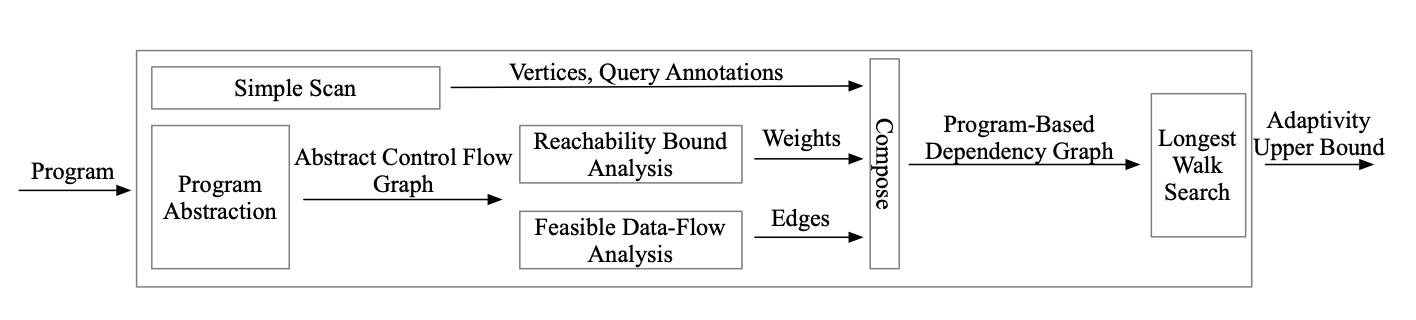
\includegraphics[width=1.0\columnwidth]{adapfun.png}
%   \vspace{-0.3cm}
%   \caption{The overview of {\THESYSTEM}}
%   \label{fig:adaptfun}
%   \vspace{-0.5cm}
% \end{figure}
%
%
\begin{enumerate}
\item  In Section~\ref{sec:abscfg}, we first construct an abstract transition graph based on $c$, by computing an abstract transition 
for every labeled command. 
This graph is used in the following sections
%  from Section~\ref{sec:pathsensitive_rb-refine} to Section~\ref{sec:pathsensitive_rb-psrbcompute} 
for computing the path-sensitive reachability-bound of a program location.
% see Section~\ref{sec:alg_vertexgen}
\item Section~\ref{sec:pathsensitive_rb-refine}
refines the multiple-paths loops in the program
% this program path sensitively, 
based on the abstract transition graph. This step produces a refined program in the form of \todo{paths sequence} which come from its abstract transition graph.
\item Section~\ref{sec:pathsensitive_rb-lbcompute} computes the ranking function / local bound for each edge in a program's abstract transition graph,
and estimates the upper bounds on every ranking function's maximum value and every edge's execution times path-insensitively.
% path-insensitive reachability upper bound for every while loop command in $c$.
\item Section~\ref{sec:pathsensitive_rb-outinalg} performs the \textbf{Outside-In} algorithm and computes
the upper bound for the execution times of \todo{certain sub-sequence} of paths in a refined program locally, named \textbf{Outside-In} bound.
% path-sensitive local bounds.
\item Section~\ref{sec:pathsensitive_rb-inoutalg} performs the \textbf{Inside-Out} algorithm and 
computes the upper bound for the execution times of
every distinct path in a refined program globally, named \textbf{Inside-Out} bound.
% abstract transition graph.
\item Section~\ref{sec:pathsensitive_rb-psrbcompute} computes the path-sensitive reachability-bound for every program point
%  in this program 
 $c$ based on the above results.
%  by
%  ?summarizing 
% the path-sensitive reachabilitybound of each edge on the abstract transition graph.
% \item The Section~\ref{sec:reachabilitybound_algorithm} computes program's reachability bound in two steps as follows.
\end{enumerate}
% Finally, with all the ingredients ready, we construct the final approximated program-based dependency graph in Section~\ref{sec:alg_graphgen}

% the algorithm  without extra static analysis technique.
% \\
% Overall, this program-based graph has a similar topology structure as 
% % the one
% % of 
% the Execution-Based Dependency Graph. It has the same
% vertices and query annotations, but approximated edges and weights. We call the graph generated by static analysis techniques, static analysis dedendency graph. 
% \item Then in the last phase in Section~\ref{sec:alg_adaptcompute}, $\THESYSTEM$
% % we compute the upper bound for adaptivity over this approximated graph:
% % , as an upper bound for
% % program's adaptivity
% computes the upper bound for adaptivity over this approximated graph.
% in the last phase of this algorithm in Section~\ref{sec:alg_adaptcompute}.
% \subsection{Adaptivity Based on Program Analysis in \THESYSTEM}
% In order to give a bound on the program's adaptivity, we first build a
% program-based data-dependency graph to {over-}approximate the
% trace-based dependency graph.  Then, we define a program-based
% adaptivity over this approximated graph, as an upper bound for
% $A(c)$.
% %
% \subsection{ $\THESYSTEM$ Analysis Algorithm}
% \subsection{Dependency Graph Estimation}
% \subsection{Vertices Estimationn}
% \label{sec:alg_vertexgen}
% The first component of every vertex in the static analysis dependency graph are actually identical as the  Execution-Based Dependency Graph, which are assigned variables in the program annotated with the unique label(line number). 
% These vertices are collected by statically scanning the program, like what we do for vertices of its Execution-Based Dependency Graph. 
% The vertices are defined formally as follows.

%   \highlight{
% \[
%     \progV^0(c) \triangleq \left\{ 
%   (x^l, w) \in \mathcal{LV} \times \mathcal{A}_{\lin}
%   ~ \middle\vert ~
%   x^l \in \lvar(c)
%   \right\}
%   \]
%   }
%   %
% where $\mathcal{A}_{\lin}$ is the set of arithmetic expressions over $\mathbb{N}$ and program's input variables. 
% The weight $w$ for every vertex will be computed in following step in Section~\ref{sec:alg_weightgen}.
% The static scanning of the programs also tells us whether one vertice(assigned variable) is assigned by a query request. We have similar definition when defining the Execution-Based Dependency Graph, 
% a set of pairs $\progF(c) \in \mathcal{P}(\mathcal{LV} \times \{0, 1\} )$ 
% % is the set of pairs 
% % The weight for each vertex in $\progV(c)$ is computed 
% mapping each $x^l \in \progV(c)$ to a flag, either $0$ or $1$, where $1$  means $x^{l}$ is a member of $ \qvar_{c}$, a set of those variables assigned with query requests, and $0$ means $x^{l}$ not in this set. It is defined formally below.

% \[\progF(c) =\left\{(x^l, n)  \in  \mathcal{LV} \times \{0, 1\} 
% ~ \middle\vert ~
% x^l \in \lvar_{c},
% n = 1 \iff x^l \in \qvar_{c} \land n = 0 \iff  x^l \not\in \qvar_{c} .
% \right\}\]
%

% \wq{To do: Add $\THESYSTEM$, a data flow analysis algorithm to scan the program and give a graph.}
% {\THESYSTEM} consists of three phases: 
% \begin{enumerate}
%     \item Generating an abstract transition graph with each edge representing an abstract event transiting between two command labels. 
%     \item Computing the value bound invariant for each variable in the event and 
%     the event transition closure over the abstract transition graph,
%     we get the reachability bound for each labeled command.
%     \item Refining the abstract transition graph with data-flow, by performing the reaching definition analysis, we generate a weighted data control flow graph.
%     \item An algorithm to find the appropriate path in the weighted data control flow graph
% \end{enumerate}

% \begin{enumerate}
%     \item An algorithm to generate a precise data control flow graph
%     \item An algorithm to perform a Reachability number analysis to calculate the weight of each node in the graph generated in phase 1.
%     \item An algorithm to find the appropriate path in the weighted data control flow graph
% \end{enumerate}

% \subsection{Edge and Weight Estimation}
% \label{sec:alg_weightedgegen}

% Since the edges of the execution-based graph of a program relies on the dependency relation, which handles both control flow and data flow, as an over-approximation of this graph, the edges of our static anlaysis dependency graph also covers these two kind of flows. We develop a feasible data flow relation to catch these two flows, in Section~\ref{sec:alg_edgegen}.


% The weight of every vertice in the execution-based graph is built on all possible execution traces.
% In order to over-approximate the weight statically but still tightly, we present a symbolic reachability bound analysis for estimation of the weight of each vertice(label) in Section~\ref{sec:alg_weightgen},
% in spirit of some reachablility bound techiniques.


% The edges and weight estimation are both performed on basis of an abstract transition graph of the program, we first show how to generate this abstract transition graph before the introduction of  the edge and weight estimation.  

% This analysis first 
%  generate an abstract transition graph
%  over all program labels, 
% in order to analyzing the data flow relations through variables assigned in every labeled command,
% and the reaching time of each variable.
% Then, it refines this control flow graph 
% % into a weighted data-dependency graph, 
% and generate the Program-Based Dependency Graph,
% through the data flow and reaching bound analysis results.
% In the last step, it finds the longest finite walk in this weighted data control flow graph w.r.t. the query variables,
% and return the number of query vertices traversed alongside.
% % \wq{To do: Add $\THESYSTEM$, a data flow analysis algorithm to scan the program and give a graph.}
% To be more specific, {\THESYSTEM} consists of five phases as follows,
% \\
% % \jl{Better to have a graph or picture of overview of the algorithm}
% \todo{graph}
% \todo{pass again}
% This analysis
% \begin{enumerate}
%     % \item Generating 
%     \item first generate 
%     an abstract transition graph
%     %  over all labels,
%     (remove?? with program's labels as vertices and abstract transitions as edges)
%     in Section~\ref{sec:abscfg},
%     % used to analyze 
%     for analyzing the weight of every vertex in $\progV(c)$ and edges between every vertex in $\progV(c)$ in the next two steps;
%     %  \ref{sec:alg_weightgen} and 
%     % \ref{sec:alg_edgegen}.

%     % which are used as program's program points,
%     %
%     \item then use the abstract transition graph generated above, 
%     compute the weight of every vertex in $\progV(c)$ by computing a symbolic reachability bound for each label in Section~\ref{sec:alg_weightgen},
%     % \\
%     \item and then use the same graph again to estimate the edges between every vertex in $\progV(c)$ by computing the feasible data flow relation between every labeled variables in Section~\ref{sec:alg_edgegen}.
  
% \end{enumerate}

\subsection{Abstract Transition Graph}
\label{sec:abscfg}

This path-sensitive reachability-bound algorithm
is performed on basis of an \emph{Abstract Transition Graph} for the program $c$.
% We first show 
This step shows how to generate the abstract transition graph $\absG(c)$ of a
program $c$ through vertices and edges constructions.
%  before the introduction of the edge and weight estimation.  
% We discuss the vertices and edge of the
% abstract transition graph for a program $c$, $\absG(c)$.

\subsubsection{Vertices Construction}
\label{sec:abscfg-vertex}
Every 
vertex corresponds to a program execution point, which is a unique
label of a command in this program.
Specifically,
the vertices of this graph is the set of $c$'s labels with the exit label ${\lex}$, 
\[ 
  \absV(c) = \lvar(c)\cup\{{\lex}\}
  \]
%  corresponding to a label command in the program.

\subsubsection{Edge Construction}
\label{sec:abscfg-edge}
  The vertices can be easily collected and the key point of the abstract
  transition graph for a program is constructing the edge set, $\absE(c)$ for a program $c$.
  It relies on the control flow analysis and the program abstraction of each command.
  %  and abstract transition (we also call it abstract event).
  To make it easy to understand, it
  is a refined control flow graph with an annotation on every edge.
  The edge set is constructed by a program abstraction method in three steps.
  \\
  In the first step, \textbf{Constraint Generation} generates the constraint
  for the expression in each program command,
  which is used as the annotation of an edge.
  \\
  In the second step, \textbf{Initial and Final State} generates two sets for each command. 
  The initial state is a set that contains the
  program point where this command \todo{starts} executing, 
  and the final state is a set
  that contains the constraint of this command
  and the continuation program points after the execution of this command.
  \\ 
  In the third step, \textbf{Abstract Event} generates a set of edges for the program.
  Each edge is a pair of initial and finial state.
  % The annotation of each edge is a constraint generated by a program abstraction method.
  % by adopting the program abstraction.
  %  method in Section 6 in~\cite{sinn2017complexity}.
  %  the program's every command.
% It is computed as follows.
  % The edge in the abstract transition graph comes from the abstract execution trace of the program. 
  % The abstract execution trace, an abstract representation of the execution, consists of a set of abstract events. 
%   The edge in the abstract transition graph comes from the program's abstract events set $\absflow(c)$.
%   Each abstract event $(l_1, dc, l_2)$ in this set represents an edge in $\absE(c)$.
%   % Then, every abstract transition in the abstraction execution trace corresponds to an edge in the abstract transition graph. In another word, the edge $(l_1, dc, l_2)$ in the abstract transition graph, represents an abstract transition 
% %  from $l_1$ to $l_2$, with a set of difference constraints $dc$. 
%  Also notice, the difference constraints generated during the abstract transition appears in the edge as annotation.
%
\paragraph{Constraint Generation}
In this step, we first show how to compute the constraints for expressions in a program $c$,
by a program abstraction method adopted from the
algorithm in Section 6 in~\cite{sinn2017complexity}.
\\
Given a program $c$,
every expression in an assignment command or in the guard of a $\eif$ or $\ewhile$ command
is transformed into a constraint.

\highlight{Notations / Formal Definitions:}
\begin{itemize}
\item Operator: $\absexpr : \mathcal{A} \cup \mathcal{B} \to DC(\mathcal{VAR}  \cup \constdom)\cup \booldom \cup \{\top\}$
%
\item Constraints $\dcdom^{\top}: DC(\mathcal{VAR}  \cup \constdom) \cup \booldom$  contains:
%
\begin{itemize}
\item Difference Constraints $DC(\mathcal{VAR}  \cup \constdom)$ is the set of all the inequality of
form $x' \leq y + v$ where $x \in \mathcal{VAR} $, 
$y \in \mathcal{VAR}$ and $v \in \constdom$.
The \emph{Symbolic Constant} set $\constdom = \mathbb{N} \cup \inpvar \cup{\infty}$
is the set of natural numbers with $\infty$ and input variables.
An inequality $x' \leq y + v$ describes that the value of $x$ in the current state is
at most the value of $y$ in the previous state plus some constant $v$.
%
\item The Boolean Expressions from the set $\booldom$
%
% \item The infinity $\top$.
\end{itemize}
\end{itemize}

\highlight{Computation Steps:}
\begin{defn}[Constraint Computation]
  \label{def:constraint_compute}
  For a program $c$, a boolean expression $\bexpr$ in the guard of a $\eif$ or $\ewhile$ command
  or an expression $\expr$ and a variable $x$
  in an assignment command $\assign{x}{\expr}$,
  % or 
  % For a boolean expression $\bexpr$ or an arithmetic expression $\aexpr$ and a variable $x$,
  the constraint $\absexpr(\bexpr, \_)$ or $\absexpr(x - v, x)$ is computed as follows,
  \[
    \begin{array}{ll} 
      \absexpr(x - v, x)  = x' \leq x - v  & x \in \grdvar \land v \in \mathbb{N} \\
      \absexpr(y + v, x)  = x' \leq y + v  & x \in \grdvar \land v \in \mathbb{Z} \land y \in (\grdvar \cup \constdom) \\
      \absexpr(v, x)  = x' \leq v + 0  & x \in \grdvar \land v \in (\grdvar \cup \constdom) \\
      \absexpr(y + v, x)  = x' \leq y + v & \\
      \grdvar = \grdvar \cup \{y\} & x \in \grdvar \land v \in \mathbb{Z} \land y \notin (\grdvar \cup \constdom)  \\
      % \absexpr(\qexpr, x)  = x' \leq 0 + Q_m & x \in \grdvar \land \qexpr \text{ is a query expression}  \\
      \absexpr(\expr, x) = x' \leq \infty  &  x \in \grdvar \land \expr \text{ doesn't have any of the forms as above} \\
      \absexpr(\expr, x) = \etrue  &  x \notin \grdvar \\
      \absexpr(\bexpr, \_) = \bexpr   & \\
      % \absexpr(y + v, x)  = x' \leq y + v & \\
      \grdvar = \grdvar \cup FV(\bexpr) &  x \in \grdvar \land \bexpr \text{ is a boolean expression} \\
    \end{array}
    \]
  \end{defn}
%
  $\grdvar$ is the set of variables used in the guard expression of every while command in the program $c$. 
  In the case 4, if a variable $x$, belonging to the set 
  $\grdvar$ is updated by a variable $y$, which isn't in this set, 
  we add $y$ into the set $\grdvar$ and repeat 
  above procedure  until $\grdvar$ and $\absexpr(\expr, x)$ is stabilized. 
  % \wq{I do not understand this sentence:-(}
  \\
Specifically 
% understanding the intuition, 
we handle a 
% simplified 
normalized expression, $x > 0$
in guards of while loop headers, and 
%  \wq{I do not understand this sentence:-(}
%  .
% \\
% The counter variables only increase, decrease or reset by expression in the form of arithmetic minus and plus (able to extend to max and min.)
the counter variable $x$ only increase, decrease or reset by 
% expression in the form of 
simple arithmetic expression (mainly multiplication, division, minus and plus (able to extend to max and min)). 
The counter variable $x$ is generalized into norm when the boolean expression $x > 0$
in $\ewhile$ doesn't have the form $x > 0$.
The way of normalizing the guards and computing the norms is adopted from the computation step 1 in Section 6.1 in paper \cite{sinn2017complexity}. 
% \\
% For more complex expression assignments, where the counter reset, or calculated from $\elog$, 
% multiplication or division, and expressions involving multiple variables, the constraint is approximated as reset of $\infty$.
% \\
% % This simplification \wq{which part we simplify here?} 
% This approximation strategy
% doesn't affect our analysis results in our examples. It is easy to extend the normalized expression 
% into more complex forms as in \cite{sinn2017complexity}, as well as the 
% counter variable manipulation with more advanced expressions.
% \\ 
% The boolean expression in the guard of $\ewhile$ command is normalized into form of $ x > 0$ where $x^l \in \lvar_c$ for some $l$.
\begin{defn}[Symbolic Expression ($\mathcal{A}_{S}$)]
  $\mathcal{A}_{S}$ is the set of all the symbolic expressions 
over $\constdom$.
% For concise, $\mathcal{A}_{\lin}$ is used as the same meaning of $EXPR(\constdom)$ in the follows, to denote the arithmetic expression 
% over the symbolic variables, (i.e., $\mathbb{N}$ with input variables).
\end{defn}
The symbolic expression set is a subset of arithmetic expressions over $\mathbb{N}$ with input variables, 
i.e., $\mathcal{A}_{S} \subseteq \mathcal{A}_{\lin}$.
% \subsubsection{Abstract Transition Graph through an Example}
\paragraph{Abstract Initial and Final State}
This step computes two sets for each command. 
The initial state is a set that contains the
program points before executing this command, which is computed by the standard initial state generation method from control flow analysis.
The final state is a set
that contains the constraint of this command and the program points after the execution of this command.
This set is enriched 
% program's initial and final states 
from the standard control flow analysis.

%
\highlight{Notations / Formal Definitions:}
\begin{itemize}
\item The abstract initial state: $\absinit(c) \in \ldom$.
%
\item The abstract Final State: $\absfinal(c) \in \mathcal{P}(\ldom \times \dcdom^{\top})$
\end{itemize}

\highlight{Computation Steps:}
\begin{itemize}
  \item The \emph{abstract initial state}, $\absinit(c) \in \mathcal{P}(\ldom)$
  for a command $c$ is the set of the initial program points.
Each point in this set is a unique program label corresponds to the command before executing this command. 
% when executing this program.
\\
Given a program $c$, its abstract initial state, $\absinit(c)$ is computed as follows,
%
\[
  \begin{array}{ll}
    \absinit(\clabel{\assign{x}{\expr}}{}^l)  & = \{l\}  \\
    \absinit(\clabel{\assign{x}{\expr}}{}^l)  & = \{l\} \\
    \absinit(\clabel{\eskip}^{l})  & = l \\
    \absinit(\eif [b]^l \ethen c_1 \eelse c_2)  & = \{l\} \\
    \absinit(\ewhile [b]^l \edo c)  & = \{l\} \\
    \absinit(c_1 ; c_2)  & = \absinit(c_1) \\
 \end{array}
 \]
%
%
\item The \emph{abstract final state} of the program $c$, 
$\absfinal(c) \in \mathcal{P}(\ldom \times \dcdom^{\top})$
is a set of pairs, $(l, dc)$ with a
program point (i.e., a label), $l$ as the first component and a constraint, 
$dc$ as the second component.
% Every pair in $\absfinal(c)$ 
The program point $l$ corresponds to the labeled command after the execution of $c$,
and the constraint $dc$ in this pair is computed by $\absexpr$ for the expression in $c$.
%  in the first step.
\\
Given a program $c$, its final state, $\absfinal(c)$ is computed as follows,
% $\absfinal(c) \in\mathcal{P}(\ldom \times \dcdom^{\top})$,
% computes the set of Abstract Final State for the command. 
 \[
  \begin{array}{ll}
    \absfinal(\clabel{\assign{x}{\expr}}{}^l)  & = \{(l, \absexpr\eapp (\expr, x))\}  \\
    %  \absfinal(\clabel{\assign{x}{\query(\qexpr)}}{}^l)  & = \{
    %   (l, x' \leq 0 + Q_m )\}  \\
     \absfinal(\clabel{\eskip}^{l})  
     & = \{(l, \top)\} \\
     \absfinal(\eif [b]^l \ethen c_1 \eelse c_2)  & = \absfinal(c_1) \cup \absfinal(c_2) \\
     \absfinal(\ewhile [b]^l \edo c)  & = \{(l, \absexpr(\bexpr, \top))\} \\
     \absfinal(c_1 ; c_2)  & =  \absfinal(c_2) \\
 \end{array}
 \]
 %
\end{itemize}
 \paragraph{Abstract Event} Each abstract event is an edge between two vertices in the abstract transition graph.
 It is generated by computing the initial state and finial state interactively for a program $c$.
 
 \highlight{Notations / Formal Definitions:}
 \begin{itemize}
  \item \emph{Abstract Event}: 
  $\absevent \in $
  $\ldom \times \dcdom^{\top} \times \ldom$
  \item \emph{Abstract Event Computation}: $\absflow \in \cdom \to \mathcal{P}( \ldom \times \dcdom^{\top} \times \ldom )$
 \end{itemize}
 Its type is defined as follows,
 \begin{defn}[Abstract Event]
   \label{def:abs_event}
   Abstract Event: 
   $\absevent \in $
   $\ldom \times \dcdom^{\top} \times \ldom$
   is a 
   % pair of abstract initial state and final state.
   triple where the first and third components are labels,
   second component is a constraint from $\dcdom^{\top}$.
   % the thrid % computed from program's abstract final and initial state, $\absfinal(c)$ and $\absinit(c)$ with formal definition, and algorithm detail in Appendix.
   %  the constraint and the third corresponds to a final state.
   \end{defn}
   In an abstract event $(l, dc, l')$ of a program $c$, 
   the first label $l \in \ldom$ corresponds to an initial state of $c$, and 
   the second label $l' \in \ldom$ with the constraint $dc\dcdom^{\top}$ correspond to an abstract final state of $c$.
  The abstract initial state is a label from $\ldom$.
%  The abstract final state is a pair from $\ldom \times \dcdom^{\top}$,  
%  where first component is a label from $\ldom$ and the second component is a constraint from $\dcdom^{\top}$.
 %
We abuse the notation $\mathcal{P}(\absevent)$ for the power set of all abstract events.

 \highlight{Computation Steps:}
\\
% The abstract event is computed for w.r.t the program in Definition~\ref{def:absevent_compute}, 
%  generated during computing its abstract execution trace, 
%  , and we have $\absflow(c) \in \mathcal{P}(\absevent)$.
%  Now, we  extract the abstract execution trace  $\absflow(c)$ for a program, which computes the 
%  The \emph{Abstract Execution Trace} for program $c$ is a s
The set of the abstract events $\absflow(c)$ for a program $c$
% .
%  Its type is formally defined 
is computed as follows in Definition~\ref{def:absevent_compute}.
 %
 \begin{defn}[Abstract Event Computation]
 \label{def:absevent_compute}
  $\absflow \in \cdom \to \mathcal{P}( \ldom \times \dcdom^{\top} \times \ldom )$
  \end{defn}
 %
%  The \emph{Abstract Execution Trace} for program $c$ is computed as follows.
%  \\
  % We now show how to compute the abstract execution trace. 
 We first append a $\eskip$ command with 
%  a symbolic label $l_e$, i.e., $\clabel{\eskip}^{l_e}$ at the end of the program $c$, and compute the $\absflow(c) = \absflow'(c')$ for $c'$, where $c' = c;\clabel{\eskip}^{l_e}$ as follows,
the label $\lex$, i.e., $\clabel{\eskip}^{l_{ex}}$ at the end of the program $c$, and construct 
the program $c' = c;\clabel{\eskip}^{l_{ex}}$.
Then, we compute the $\absflow(c) = \absflow'(c')$ for $c'$ as follows,
 %
 {\footnotesize
 \[
   \begin{array}{ll}
      \absflow'(\clabel{\assign{x}{\expr}}{}^l)  & = \emptyset  \\
      \absflow'(\clabel{\assign{x}{\query(\qexpr)}}{}^l)  & = \emptyset  \\
      \absflow'([\eskip]^{l})  & = \emptyset \\
      \absflow'(\eif [b]^l \ethen c_t \eelse c_f)  & =  \absflow'(c_t) \cup \absflow'(c_f)
        \\ & \quad 
        \cup \{(l, \absexpr(\bexpr, \top),  \absinit(c_t) ) ,  (l, \absexpr(\neg\bexpr, \top), \absinit(c_f)) \} \\
       \absflow'(\ewhile [b]^l \edo c_w)  & =  \absflow'(c_w) \cup \{(l, \absexpr(\bexpr, \top), \absinit(c_w)) \} 
       \\ & \quad 
       \cup \{(l', dc, l)| (l', dc) \in \absfinal(c_w) \} \\
       \absflow'(c_1 ; c_2)  & = \absflow'(c_1) \cup  \absflow'(c_2) 
       \\ & \quad 
       \cup \{ (l, dc, \absinit(c_2)) | (l, dc) \in \absfinal(c_1) \} \\
   \end{array}
   \]
   }
   Notice $\absflow'([x := \expr]^{l})$, $\absflow'([x := \query(\qexpr)]^{l})$ and $\absflow'([\eskip]^{l})$ are all empty set. 
   For every event $\event$ with label $l$ in an execution trace $\trace$ of program $c$, 
   there is an abstract event in program's abstract execution trace of form $(l, \_, \_)$.  
   We also show the soundness of the abstract events computation in Appendix.

 \highlight{Theorem Guarantee:}
   \begin{lem}[Soundness of the Abstract Events Computation]
     \label{lem:abscfg_sound}
   Given a program ${c}$, we have:
   %
   \[
     \begin{array}{l}
       \forall \vtrace_0, \trace \in \mathcal{T} ,  \event = (\_, l, \_) \in \eventset \st
   \config{{c}, \trace_0} \to^{*} \config{\eskip, \trace_0 \tracecat \vtrace} 
   \land \event \in \trace 
   \\
   \qquad \implies \exists \absevent = (l, \_, \_) \in (\ldom\times \dcdom^{\top} \times \ldom) \st 
   \absevent \in \absflow(c)
   \end{array}
   \]
   \end{lem}
%    This lemma is proved formally in Appendix~\ref{apdx:pathinsensitive_rb_soundness}.
% For every event $\event$ with label $l$ in an execution trace $\trace$ of program $c$, 
% there is an abstract event in program's abstract events computation of form $(l, \_, \_)$. 
This lemma is proved formally in Lemma~\ref{lem:abscfg_sound} in Appendix~\ref{apdx:pathinsensitive_rb_soundness}.
\\
For every program point $l$ corresponding to an assignment command in a program $c$,
%  $x^l \in \lvar_c$, 
there is a unique abstract event in the program's abstract events set $\absevent \in \absflow(c)$ of form $(l, \_, \_)$. 
\begin{lem}[Uniqueness of the Abstract Events Computation]
  \label{lem:abscfg_unique}
Given a program ${c}$, we have:
%
\[
  \begin{array}{l}
    \forall \vtrace_0, \trace \in \mathcal{T} ,  \event = (\_, l, \_) \in \eventset^{\asn} \st
\config{{c}, \trace_0} \to^{*} \config{\eskip, \trace_0 \tracecat \vtrace} 
\land \event \in \trace 
\\
\qquad \implies \exists! \absevent = (l, \_, \_) \in (\ldom\times \dcdom^{\top} \times \ldom) \st 
\absevent \in \absflow(c)
\end{array}
\]
\end{lem}
This lemma and proof is also 
formalized in Lemma~\ref{lem:absevent_unique} in Appendix~\ref{apdx:pathinsensitive_rb_soundness}.

  \paragraph{Edge Construction}
The edge for $c$'s abstract transition graph is constructed formally as follows,
  \[
    \absE(c) = \{(l_1, dc, l_2) | (l_1, dc, l_2) \in \absflow(c)\}
    \]
The edge set is constructed simply by computing the program's abstract events set, $\absflow(c)$.
%   Each abstract event $(l_1, dc, l_2)$ in this set represents an edge in $\absE(c)$.
%   % Then, every abstract transition in the abstraction execution trace corresponds to an edge in the abstract transition graph. In another word, the edge $(l_1, dc, l_2)$ in the abstract transition graph, represents an abstract transition 
% %  from $l_1$ to $l_2$, with a set of difference constraints $dc$. 
%  The constraints generated in the abstract event appears in the edge as annotation.
% We have a pre-processing algorithm to go through the programs and returns the list of labels associating with a loop and whose visiting times need to be analyzed.
%
\subsubsection{Abstract Transition Graph Construction} 
With the vertices $\absV(c)$ and edges $\absE(c)$ ready, we construct the abstract transition graph, formally in
% Through a program $c$'s abstract events computation, its abstract transition graph is computed in 
Definition~\ref{def:abs_cfg}.
%
\begin{defn}[Abstract Transition Graph]
\label{def:abs_cfg}
Given a program $c$, 
its \emph{abstract transition graph} $\absG(c) =(\absV(c), \absE(c))$ is computed as follows,
\\
$\absE(c) = \{(l_1, dc, l_2) | (l_1, dc, l_2) \in \absflow(c)\}$,
\\
$\absV(c) = \lvar(c)\cup\{\lex\}$
% \\
%  $\absW(c) 
% \triangleq \left\{ (l, w) \in \mathbb{L} \times EXPR(\constdom) \right\}$.
\end{defn}
% \\
% Notice we also define the $\absW(c)$ in this graph without giving an actual value.
% This $\absW(c)$ is the set of weight for every 
% % vertex 
% label. 
% The weight $w \in EXPR(\constdom)$ is a symbolic expression over the symbolic constant, 
% which is the estimated upper bound on the number of visiting time for every program point
% through the reachability bound analysis as follows.
%
% $EXPR(\constdom)$ is the set of all the symbolic expressions 
% over $\constdom$, which is a subset of arithmetic expressions over $\mathbb{N}$ with input variables.
% For concise, $\mathcal{A}_{\lin}$ is used as the same meaning of $EXPR(\constdom)$ in the follows, to denote the arithmetic expression 
% over the symbolic variables, (i.e., $\mathbb{N}$ with input variables).
\subsubsection{Abstract Transition Graph through An Example}
\label{sec:abscfg_example}
% 
% Look at the two-round example again, its generated abstract control is shown as in Figure~\ref{fig:adapfun_tworound}(a).
% In this abstract transition graph, every vertex is a label,
% corresponding to a label command in the program.
% Each directed 
% edge represents an abstract transition 
% between two program points, 
% i.e., the labels of two commands (we call the labels also program point and they refer to the same thing), 
% where the second labeled command will be executed after execution of the command with first label.
% For example, the edge $0, a \leq 0, 1$ on the top, represents,
% from location $0$, the command 
% $\clabel{\assign{a}{0}}^0$ is executed with next continuation location $1$,
% where the 
% command $\clabel{\assign{j}{k}}^1$ will be executed next.
% The constraint $a \leq 0$ is generated by abstracting from the assignment command $\assign{a}{0}$,
% representing that value of $a$ is less than or equals to $0$ after 
% location $0$ before executing command at line $1$.
% %
% The same way for the rest edges' constructions.
%
\begin{example}[The Abstract Control Flow Graph for A Simple While Loop Program]
  \label{ex:whileSim_abscfg}
    For the simple while loop example program, 
its abstract control flow graph is shown as in Figure~\ref{fig:whileSim_abscfg}(b).
For example, the edge $(0, a' \leq 0, 1)$ on the top, tells us the command 
$\clabel{\assign{a}{0}}^0$ is executed with next continuation point $1$,
where the 
command $\clabel{\assign{j}{k}}^1$ will be executed next.
The constraint $a' \leq 0$ is a difference constraint, generated by abstracting from the assignment command $\assign{a}{0}$.
It represents that the value of $a$ is less than or equals to $0$ after 
execution of $\clabel{\assign{a}{0}}^0$ and before executing $\clabel{\assign{j}{k}}^1$.
The difference constraint is an inequality relation, 
the left-hand side of the inequality $x'$ denotes the variable $x$
after executing the command at $l$
and the right-hand side describes the variable $x$ in the state before the execution. 
Look at the $a' < a+x $ on the edge $5$ to $2$, which describes the execution of the command at line $5$, 
which is an assignment $a' = a+x$. The $a'$ on the left side of $a' < a+x$ represents the value of $a$ after the assignment,
while the right-hand side $a$ stores the value before the assignment. 
% $top$ means there is no assignment executed, for example, 
I have 
The boolean constraint $j \leq 0 $ on the edge $2 \to 6$, 
represents the negation of the testing guard $j > 0$
in the $\ewhile$ command with loop header at line $2$.
%
% The same way for the rest edges' constructions.
\begin{figure} 
  \centering
  \begin{subfigure}{.7\textwidth}
  \begin{centering}
  {\small
  $
  \kw{whileSim(k)} \triangleq
    \begin{array}{l}
        \clabel{ \assign{a}{0}}^{0} ;   
              \clabel{\assign{j}{k} }^{1} ;\\
              \ewhile ~ \clabel{j > 0}^{2} ~ \edo ~ 
              \Big(
               \clabel{\assign{x}{j} }^{3}  ;
               \clabel{\assign{j}{j-1}}^{4} ;
              \clabel{\assign{a}{x + a}}^{5}  \Big);\\
              \clabel{\assign{l}{k * a} }^{6}
          \end{array}
  $
  }
  \caption{}
  \end{centering}
  \end{subfigure}
    \begin{subfigure}{.45\textwidth}
    \begin{centering}
  \begin{tikzpicture}[scale=\textwidth/20cm,samples=200]
  \draw[] (-7, 10) circle (0pt) node{{ $0$}};
  \draw[] (0, 10) circle (0pt) node{{ $1$}};
  \draw[] (0, 7) circle (0pt) node{\textbf{$2$}};
  \draw[] (0, 4) circle (0pt) node{{ $3$}};
  \draw[] (0, 1) circle (0pt) node{{ $4$}};
  \draw[] (-7, 1) circle (0pt) node{{ $5$}};
  % Counter Variables
  \draw[] (6, 7) circle (0pt) node {\textbf{$6$}};
  \draw[] (6, 4) circle (0pt) node {{ $\lex$}};
  %
  % Control Flow Edges:
  \draw[ thick, -latex] (-6, 10)  -- node [above] {$a' \leq 0$}(-0.5, 10);
  \draw[ thick, -latex] (0, 9.5)  -- node [left] {$j' \leq k$} (0, 7.5) ;
  \draw[ thick, -latex] (0, 6.5)  -- node [right] {$j > 0$}  (0, 4.5);
  \draw[ thick, -latex] (0, 3.5)  -- node [right] {$x' \leq j$} (0, 1.5) ;
  \draw[ thick, -latex] (-0.5, 1)  -- node [above] {$j' \leq j - 1$} (-6, 1) ;
  \draw[ thick, -latex] (-6, 1.5)  -- node [left] {$a' \leq x + a$} (-0.5, 7)  ;
  \draw[ thick, -latex] (0.5, 7)  -- node [above] {$ j \leq 0 $}  (5.5, 7);
  \draw[ thick, -latex] (6, 6.5)  -- node [right] {$l' \leq k * a$} (6, 4.5) ;
  \end{tikzpicture}
  \caption{}
    \end{centering}
    \end{subfigure}
    \begin{subfigure}{.45\textwidth}
      \begin{centering}
    %   \todo{abstract-cfg for two round}
    \begin{tikzpicture}[scale=\textwidth/20cm,samples=200]
    \draw[] (-10, 10) circle (0pt) node{{ $0: 1$}};
    \draw[] (0, 10) circle (0pt) node{{ $1: 1$}};
    \draw[] (0, 7) circle (0pt) node{\textbf{$2: k$}};
    \draw[] (0, 4) circle (0pt) node{{ $3: k$}};
    \draw[] (0, 1) circle (0pt) node{{ $4: k$}};
    \draw[] (-10, 1) circle (0pt) node{{ $5: k$}};
    % Counter Variables
    \draw[] (6, 7) circle (0pt) node {\textbf{$6: 1$}};
    \draw[] (6, 4) circle (0pt) node {{ $\lex: 1$}};
    %
    % Control Flow Edges:
  \draw[ thick, -latex] (-8, 10)  -- node [above] {$a' \leq 0$}(-1.5, 10);
  \draw[ thick, -latex] (0, 9.5)  -- node [left] {$j' \leq k$} (0, 7.5) ;
  \draw[ thick, -latex] (0, 6.5)  -- node [right] {$j > 0 $}  (0, 4.5);
  \draw[ thick, -latex] (0, 3.5)  -- node [right] {$x' \leq j$} (0, 1.5) ;
  \draw[ thick, -latex] (-1.5, 1)  -- node [above] {$j' \leq j - 1$} (-8, 1) ;
  \draw[ thick, -latex] (-8, 1.5)  -- node [left] {$a' \leq x + a$} (-1.5, 7)  ;
  \draw[ thick, -latex] (1.5, 7)  -- node [above] {$j \leq 0 $}  (4.5, 7);
  \draw[ thick, -latex] (6, 6.5)  -- node [right] {$l' \leq k * a$} (6, 4.5) ;
    \end{tikzpicture}
    \caption{}
      \end{centering}
      \end{subfigure}
    \caption{(a) The Simple While Loop Example Program $\kw{whileSim(k)}$
    (b) The abstract control flow graph for $\kw{whileSim(k)}$  
    (c) The abstract control flow graph with the path insensitive reachability bound for $\kw{whileSim(k)}$.}
    \label{fig:whileSim_abscfg}
  \end{figure}
\end{example}
%
\subsection{\highlight{Program Refinement}}
\label{sec:pathsensitive_rb-refine}
In order to analyze the reachability bound path-sensitively, this step refines the program based on its abstract transition graph in three steps.
%
\paragraph{Simple Transition Path} This step computes the set of all \emph{simple transition paths} for a program $c$.
\\
%
% It either
A simple transition path, $\tpath \in \paths(\absG(c))$ for a program c is
a path in the abstract transition graph of $c$ that is either,
\begin{itemize}
  \item a simple cyclic path, which starts and ends at the same loop header at location $l$, 
  and visits only locations inside the natural loop of $l$ at most once;
  %  only one loop (without any nested loop) starting from a loop header at location $l$ and go back to the same $l$;
  \item or an acyclic path, which starts from a loop header $l$ 
  % (or the program entrance $l_0$)
and ends with a different loop header $l'$;
%  (or the program's exists $\lex$).
\item or an acyclic path, which starts from a loop header $l$ 
% (or the program entrance $l_0$)
and ends the program exit $\lex$;
%  (or the program's exits $\lex$).
\item or an acyclic path, which starts from the program entrance $0$
% (or the program entrance $l_0$)
and ends with a loop header $l$;
%  (or the program's exits $\lex$).
\item or an acyclic path, which starts from the program entrance $0$
% (or the program entrance $l_0$)
and ends the program exit $\lex$;
%  (or the program's exits $\lex$).
\end{itemize}
  \begin{defn}[Simple Tansition Path]
  A simple transition path
  $\tpath \in \paths(\absG(c))$, is a path on this program's abstract transition graph $\absG(c)$ with 
  \begin{itemize}
  \item a vertices sequence $(l_0, \cdots, l_n)$, where $l_i \in \lvar(c)$ for every $i = 0, \cdots, n$ and
  %
  \item an edge sequence $(e_1, \cdots, e_n)$, where $e_i = (l_{i - 1}, dc_i, l_{i}) \in \absE(c)$ for every $i = 1, \cdots, n$,
  \end{itemize}
  %
  satisfying:
  \begin{itemize}
    \item $l_i \neq l_j$ for every $l_i = l_0, \cdots, l_n$ and $l_j = l_0, \cdots, l_{n - 1}$,
    \item $l_0$ is either the program point of a loop header or the program entrance ($l_0 = 0$),
    \item and $l_n$ is either the program point of a loop header or the program exit ($l_n = \lex$).
  \end{itemize}
  \end{defn}

  % For the part of the graph not in any SCC:

  % and end of $p'$ are both $l$;
  % \\
  %
% \item 
\paragraph{Repeat Pattern.} This step computes the set of all the \emph{repeat patterns} for every while loop in a program $c$.
\\
% A \emph{Repeat Pattern} ($\rpattern \in \mathcal{P}({\absG(c)})$)
% is either a simple path or sequence of repeat patterns of this program $c$. 
% % \[
% %   \rpattern := \tpath ~|~ \rprepeat(\rpattern) ~|~ \rpattern; \rpattern
% % \]
% Every $\rpattern'$ with the annotation $\rprepeat$, (for example, $\rpattern = \rprepeat(\rpattern')$)
% can consecutively execute at least twice.
% Every two sub-repeat patterns following each other in a $\rpattern$ can execute in sequence, for example in $\rpattern = \rpattern_1; \rpattern_2$,
% $\rpattern_2$ can execute after $\rpattern_1$.
% Every sub-repeat patterns in the sequence are distinct.
% \highlight
% {
  A \emph{Repeat Pattern},
  $\rpattern \in \mathcal{P}(\paths({\absG(c)}))$ for a while loop in program $c$ is
% is either a simple path or sequence of repeat patterns of this program $c$. 
% is a sequence of simple transition paths with annotations $\rprepeat$
% it is a simple path or
% \\
%  ==> 
a sequence of simple transition paths $\tpath$ with annotations $\rprepeat$ on certain sub-sequences,
$\rpattern = \rpattern_0; \cdots; \rpattern_n$
% or a sub \emph{repeat pattern} $\rpattern'$ with annotation $\rprepeat$,
% or a sequence of sub \emph{repeat pattern}s $\rpattern_1; \cdots; \rpattern_n$ 
satisfying that:
% \[
%   \rpattern := \tpath ~|~ \rprepeat(\rpattern) ~|~ \rpattern; \rpattern
% \]
\\
1. if a sub-sequence $\rpattern'$ has the annotation $\rprepeat$, i.e., $\rprepeat(\rpattern')$,
then \highlight{it always executes consecutively} without being interleaved until its invariant is false;
% can consecutively execute at least twice w.r.t. some initial trace.
\\
2. every sub-sequence, $\rpattern_i$ in this repeat pattern $\rpattern_0; \cdots; \rpattern_n$,
%  $\rpattern$ is a sequence of sub-repeat patterns,
% i.e.,  $\rpattern = \rpattern_0; \cdots; \rpattern_n$,
% then 
% every in this sequence 
can execute
after the previous $\rpattern_{i - 1}$'s execution finished.
% \todo{ ==> iterated until end}.
%  following each other in this sequence
% % i.e., $\rpattern_1; \rpattern_2$, 
% can execute after each other,
% % can execute in sequence, for example in ,
% i.e., 
% $\rpattern_i$ can execute after $\rpattern_{i - 1}$ for every $i = 1, \cdots, n$.
% $\rpattern_2$ can execute after $\rpattern_1$.
\\
3. Every sub-sequence is distinct.
% }
% \\
% \todo{
%   A \emph{Repeat Pattern},
%   $\rpattern \in \mathcal{P}(\paths({\absG(c)}))$ for a program $c$
% % is either a simple path or sequence of repeat patterns of this program $c$. 
% % is a sequence of simple transition paths with annotations $\rprepeat$
% % it is a simple path or
% is either a simple transition paths $\tpath$,
% or a sub \emph{repeat pattern} $\rpattern'$ with annotation $\rprepeat$,
% or a sequence of sub \emph{repeat pattern}s $\rpattern_1; \cdots; \rpattern_n$ satisfying,
% % \[
% %   \rpattern := \tpath ~|~ \rprepeat(\rpattern) ~|~ \rpattern; \rpattern
% % \]
% \\
% 1. If $\rpattern$ has the annotation $\rprepeat$, i.e., $\rprepeat(\rpattern)$,
% then can consecutively execute at least twice w.r.t. some initial trace.
% \\
% 2. If $\rpattern$ is a sequence of sub-repeat patterns,
% i.e.,  $\rpattern = \rpattern_0; \cdots; \rpattern_n$,
% then every two sub-repeat patterns following each other in this sequence
% % i.e., $\rpattern_1; \rpattern_2$, 
% can execute after each other,
% % can execute in sequence, for example in ,
% i.e., 
% $\rpattern_i$ can execute after $\rpattern_{i - 1}$ for every $i = 1, \cdots, n$.
% % $\rpattern_2$ can execute after $\rpattern_1$.
% \\
% 3. Every sub-repeat pattern in a sequence is distinct.
% }
%  , i.e.,
% $rprog_i, rprog_j \in \rprog_1; \cdots; \rprog_n$, $\rprog_i \neq \rprog_j$.
% \\
% \begin{defn}[Repeat Pattern]
%   A \emph{Repeat Pattern} is a simple path or a sequence of \emph{Repeat Pattern}
%   \[
%     \rprog := \tpath ~|~ \rprepeat(\rprog) ~|~ \rprog; \rprog
%   \] 
%   satisfying,
%   \begin{itemize}
%   \item $\rprog$ can consecutively execute at least twice, and
%   \item
%   for every 
%   $\rprog_i, \rprog_j \in \rprog_1; \cdots; \rprog_n$, $\rprog_i \neq \rprog_j$.
%   \end{itemize}
% \end{defn}
%

\highlight{\textbf{Formal Definition:}}
\begin{defn}[Repeat Pattern]
  \label{def:repeat-pattern}
  % Given a abstract transition graph $\absG(c)$,
  % $\rpattern$ is a \emph{Repeat Pattern} of $\absG(c)$ if and only if, 
  A \emph{Repeat Pattern},
  $\rpattern \in \mathcal{P}(\paths({\absG(c)}))$ for a while loop in a program $c$
% is either a simple path or sequence of repeat patterns of this program $c$. 
  is
  % \todo{
  % % it is a simple path or
  % is either a simple transition paths $\tpath$,
  % or a sub \emph{repeat pattern} $\rpattern'$ with annotation $\rprepeat$,
  % or a sequence of sub \emph{repeat pattern}s $\rpattern_0; \cdots; \rpattern_n$ ==> }
  \highlight{a sequence of simple transition paths $\tpath$ with annotations $\rprepeat$ on certain sub-sequences,
  $\rpattern = \rpattern_0; \cdots; \rpattern_n$
  }
  % a sequence of \emph{repeat pattern}
  % has the following forms,
  % \[
  %   \tpath ~|~ \rprepeat(\rpattern) ~|~ \rpattern; \rpattern
  % \] 
  % and 
  satisfying that,
  \begin{itemize}
  \item every sub-sequence is distinct, 
  % i.e., if $\rpattern = \rpattern_0; \cdots; \rpattern_n$, then
  % $\rpattern_i, \rpattern_j \in \rpattern_1; \cdots; \rpattern_n$, 
  $\rpattern_i \neq \rpattern_j$ for every $i, j = 0, \cdots, n$;
  \item 
  % \todo{every sub pattern with the annotation $\rprepeat$
  % can consecutively execute at least twice in $c$
  % %  when executing this program $c$ 
  % w.r.t. some initial trace, i.e., 
  % if $\rpattern = \rprepeat(\rpattern')$, 
  % then $\rpattern'$ can consecutively execute at least twice in $c$
  % under some initial traces,}
  % \\
  \highlight{every sub-sequence $\rpattern'$ that has the annotation $\rprepeat$,
  i.e., $\rprepeat(\rpattern')$
  % if and only if
  always executes consecutively without being interleaved until its invariant is false under all possible initial traces;}
  \item 
  % and every two sub patterns following each other in this sequence can execute after each other w.r.t some initial trace,
  % i.e., if $\rpattern = \rpattern_0; \cdots; \rpattern_n$, then for every $i = 1, \cdots, n$,
  % $\rpattern_i$ can execute after $\rpattern_{i - 1}$ under some initial trace.
  % \\
  \highlight{
    % In a repeat pattern $\rpattern = \rpattern_0; \cdots; \rpattern_n$,
  every sub-sequence $\rpattern_i \in \rpattern$ can execute
  after the previous $\rpattern_{i - 1}$'s execution (or iteration) is finished.}
  \end{itemize}
\end{defn}
\highlight{\textbf{Improvement Discussion:}
\\
The improvement comes from the annotation $\rprepeat$ on the sub-sequence
that always consecutively execute without being interleaved until its invariant is false.
% In additional to guarantee the execution orders of the sub-sequences following each other,
This is an additional guarantee on the execution orders of multiple paths in a while loop.
The $\rprepeat(\rpattern')$ further refines the execution order
if there are more than one path can execute after $\rpattern'$.
% ? can execute after each other,
\\
In comparison to the traditional multiple-paths refinement methods,
\\
the contextualization method in~\cite{ZulegerGSV11} only build the relations between pairs of
simple transition paths if they can execute after each other, which is imprecise if there are multiple paths
can execute after a same path.
\\
The program refinement algorithm in ~\cite{GulwaniJK09} has the same annotations on some transition paths,
but they only has the guarantee that
the annotated path can execute multiple times.
In this sense, their method is imprecise in the same case as the contextualization method.
}
\\
%
We aim to compute the repeat patterns for every while loop in a program soundly.
\\
\highlight{\textbf{Computation Steps Summary:}}
\begin{enumerate}
  \item Checking the invariant (precondition and post-condition) of every simple transition path,
  \item Finding the multiple paths for each loop as its initial repeat pattern set.
  \item For each set of a loop, computing the repeat pattern set for this loop:
  \begin{enumerate}
    \item Adding annotation on a sequence if it must execute consecutively without being interleaved until its invariant is false.
    \item Recursively checking the invariant (precondition and post-condition) of every sequence,
    $\rpattern$ in the output set.
    Appending a sequence to the other if its execution condition
    %  of the first one
    is true after the other's executing condition is false and it is different from every sub-sequence in the other one.
    \item Repeating the two steps until the output set is stabilized.
  \end{enumerate}
\item Repeating the two steps until the output set is stabilized.
\end{enumerate}

\highlight{\textbf{Pseudocode:}}
\begin{algorithm}
\caption{
{Repeat Pattern Computation - Efficient}
\label{alg:repeat-pattern}
}
\begin{algorithmic}[1]
\REQUIRE the abstract transition graph $\absG(c)$
% the target while loop with label $l$.
\STATE  \textbf{Init} $W(c) = \{\tpath_1, \cdots, \tpath_m\}$ is initialized as a set of all the simple transition paths in $\absG(c)$.
% \\
% \qquad Finding all simple transition paths $\tpath_1, \cdots, \tpath_m \in \absG(c)$.
% \STATE  
% \textbf{For} every simple transition paths $\tpath_1, \cdots, \tpath_m$:
% %  having the same starting and ending label:
% \\
% \quad Generating
% $\rpattern_{i} = \tpath_i$ and add into $R(c)$.
%  otherwise $\rpattern_i = \tpath_i$.
% \\
% \quad Adding $\rpattern_{i}$ into $R(c)$.
\STATE  \textbf{Loop} until $W(c)$ is stabilized.
\STATE    \quad For each while loop that has the header at $l$, find all $\rpattern_i \in W(c)$ having the same starting and ending program point $l$,
      \\  \quad \quad Generating a set $RP(l) = \{\rpattern ~|~ \rpattern \in R(c) \land \rpattern = l \to \cdots \to l\}$ for this loop;
\STATE    \quad \quad Computing Loop Closure $LRP(l)$ from Algorithm~\ref{alg:loop-repeat-pattern} and updating $W(c) = (W(c) \setminus RP(l))$;
% \STATE  \quad \quad Generating $\rpattern_{i}' = \rprepeat(\rpattern_i)$ if $\rpattern_i$ can consecutively execute twice.
\STATE  \quad \quad  \textbf{For}  every  $\rpattern_i \in W(c)$ ending at $l$ and $\rpattern_j \in W(c)$ starting at $l$
\STATE  \quad \quad \quad Updating $W(c) = W(c)  \cup \{\rpattern_i \to \rpattern_j\} \setminus \{\rpattern_i, \rpattern_j\}$ 
%  \\ \quad \quad if $\rpattern_i$ ending at $l$ and $\rpattern_j$ starting at $l$.
% \STATE  \quad \textbf{For} every repeat pattern $\rpattern_1, \cdots, \rpattern_m \in R(c)$
% \STATE \quad \quad  Generate $\rpattern' = \rpattern_{i}; \rpattern_{j} $ 
% if the execution condition of $\rpattern_{j}$
% is true after $\rpattern_{j}$'s executing condition is false.
\RETURN $LRP(l)$ for every while loop with its header at $l$ and $W(c)$.
\end{algorithmic}
\end{algorithm}
%
\begin{algorithm}
  \caption{
{Repeat Pattern Computation -- Accurate}
\label{alg:repeat-pattern-complete}
}
\begin{algorithmic}[1]
\REQUIRE the abstract transition graph $\absG(c)$
% the target while loop with label $l$.
\STATE  \textbf{Init} $W(c) = \{\tpath_1, \cdots, \tpath_m\}$ is initialized as a set of all the simple transition paths in $\absG(c)$.
% \\
\STATE  \textbf{Loop} until $W(c)$ is stabilized.
\STATE    \quad For each while loop that has the header at $l$, find all $\rpattern_i \in W(c)$ having the same starting and ending program point $l$,
\\  \quad \quad Generating a set $RP(l) = \{\rpattern ~|~ \rpattern \in R(c) \land \rpattern = l \to \cdots \to l\}$ for this loop;
\STATE    \quad \quad Computing Loop Closure $LRP(l)$ from Algorithm~\ref{alg:loop-repeat-pattern} and updating $W(c) = (W(c) \setminus RP(l))$
      % \STATE  \quad \quad Generating $\rpattern_{i}' = \rprepeat(\rpattern_i)$ if $\rpattern_i$ can consecutively execute twice.
\STATE    \quad \quad \textbf{For} every $\rpattern_l \in LRP(l)$ and every  $\rpattern_i \in W(c)$ ending at $l$ and $\rpattern_j \in W(c)$ starting at $l$:
\STATE  \quad \quad \quad  Updating $W(c) = W(c) \cup \{\rpattern_i + \rpattern_l + \rpattern_j\} \setminus \{\rpattern_i, \rpattern_j\}$ 
  % \\ \quad \quad \quad if $\rpattern_i$ ending at $l$ and $\rpattern_j$ starting at $l$.
% \STATE  \quad \textbf{For} every repeat pattern $\rpattern_1, \cdots, \rpattern_m \in R(c)$
% \STATE \quad \quad  Generate $\rpattern' = \rpattern_{i}; \rpattern_{j} $ 
% if the execution condition of $\rpattern_{j}$
% is true after $\rpattern_{j}$'s executing condition is false.
\RETURN $LRP(l)$ for every while loop with its header at $l$ and $W(c)$.
\end{algorithmic}
\end{algorithm}
%
\highlight{\textbf{Algorithms' Theorem Guarantee Discussion:}}
\begin{enumerate}
  \item
Algorithm~\ref{alg:repeat-pattern}:
\\
\emph{Soundness}
% on the step $5$ in Algorithm~\ref{alg:repeat-pattern}.
% \\
% This step doesn't unfold the nested loop when it generates multiple paths for the outer loop.
% Specifically, this 
% The step in line:5 step connects  $\rpattern_i +\rpattern_j$ directly
% instead of $\rpattern_i + \rpattern_l + \rpattern_j$ for the nested $\rpattern_l \in LRP(l)$. 
% This step reduces the algorithm complexity.
% This step is sound because every nested $\rpattern_l$
% has the same invariant given they are all in the same loop starting from and ending at the same location $l$.
% But this step is inaccurate because different nested $\rpattern_l$ can result in different repeat patterns of the outside loop.
There are two steps which generate new repeat patterns.
The step in line:5 step connects  $\rpattern_i +\rpattern_j$ directly
% instead of $\rpattern_i + \rpattern_l + \rpattern_j$ for the nested $\rpattern_l \in LRP(l)$. 
% This step reduces the algorithm complexity.
This step is sound because every nested $\rpattern_l$
has the same invariant given they are all in the same loop starting from and ending at the same location $l$.
The step in line:6 generates sequence of two sub repeat patterns if they execute after each other.
This step is also sound because by checking their invariant we can compute this soundly.
% But this step is inaccurate because different nested $\rpattern_l$ can result in different repeat patterns of the outside loop.
\\
\emph{Over-Approximation}
The step in line:5 of Algorithm~\ref{alg:repeat-pattern} doesn't unfold the nested loop when it generates multiple paths for the outer loop.
Specifically, this step connects  $\rpattern_i +\rpattern_j$ directly
instead of $\rpattern_i + \rpattern_l + \rpattern_j$ for the nested $\rpattern_l \in LRP(l)$. 
In this sense, it over-approximate the repeat patterns.
Because different nested $\rpattern_l$ can result in different repeat patterns of the outside loop.
\\
\emph{Efficiency}
Again the step in line:5 increases the efficiency because it avoids the unfolding and reduces  the recursion.
\\
The program refinement algorithm in paper~\cite{GulwaniJK09} uses this strategy as well in refining each while loop without unfolding the nested loop.
Specifically in their Flatten operation in Definition~4.1.
\item
Algorithm~\ref{alg:repeat-pattern-complete}: 
\\
\emph{Soundness}
This version guarantee the soundness in the same way as Algorithm 1.
\\
\emph{Reduce the Over-Approximation}
The step in line:6
unfolds the nested loop.
% \\
Then it generates multiple paths for outer loops by connecting $\rpattern_i + \rpattern_l + \rpattern_j$ for every nested $\rpattern_l \in LRP(l)$. 
% It increases the algorithm complexity because it unfolds the nested loop.
It increases accuracy because every nested repeat pattern $\rpattern_l$
will be refined by concatenating with the outer loop.
\\
\emph{Inefficiency}
The step in line:6 increases the algorithm complexity because it unfolds the nested loop.
% The program refinement algorithm in paper~\cite{GulwaniJK09} uses this strategy as well in refining each while loop without unfolding the nested loop.
% Specifically in their Flatten operation in Definition~4.1.
% The accuracy and inefficiency discussion on the step $6$ in Algorithm~\ref{alg:repeat-pattern-complete}.
% In this version, the loop at line $5$ unfolds the nested loop.
% \\
% This step generates multiple paths for outer loops by connecting $\rpattern_i + \rpattern_l + \rpattern_j$ for every nested $\rpattern_l \in LRP(l)$. 
% It increases the algorithm complexity because it unfolds the nested loop.
% But it increases accuracy because every nested repeat pattern $\rpattern_l$ will be checked by concatenate with the outer loop.
% has the same invariant given they are all in the same loop starting from and ending at the same location $l$.
% But this step is incomplete because different $\rpattern_l$ can result in different iteration numbers of the outside loop.
\item Algorithm~\ref{alg:loop-repeat-pattern}: 
% The accuracy and termination discussion.
\\
\emph{Termination}
% \\
Line: $4$ and $7$ are the two steps where the output set $R(c)$ increases
% is added with new elements.
\\
In step $4$, a new pattern is added and the old one is removed in the same time.
So the size of $R(c)$ doesn't change.
\\
Line $7$ adds a new pattern into the output set and increases $R(c)$'s size by 1. 
It is sufficient to show that this step
% $7$ will not 
doesn't add the same pattern into $R(c)$ twice.
We first assume a new pattern $\rpattern'$ is added into $R(c)$ at step $7$, 
%
% If a new pattern $\rpattern'$ is added into $R(c)$ at step $7$, 
then line $4$ will check if $\rpattern'$ will always consecutively iterating to the end.
% \\%
There are two cases.
If ``yes'', then line $4$ will add $\rprepeat(\rpattern')$ into $R(c)$ and remove $\rpattern'$ from $R(c)$.
In this case, line $7$ will not add the same $\rpattern'$ again because it is a sub-sequence of $\rprepeat(\rpattern')$.
% in any sequence that it shows up.
% Because when it identifies the pattern $\rpattern'$, but $\rpattern'$ will not be added into $R(c)$ because
% it is a sub pattern of $\rprepeat(\rpattern')$.
% \\%
If ``no'', then line $4$ will not update the $R(c)$. 
In this case, the line $7$ will not identify any new repeat patterns. So the output set will not change and the algorithm terminates.
%  $\rpattern'$ again, $\rpattern'$ will not be added into $R(c)$ because
% it is already there.
\\
\emph{Soundness} 
The soundness is guaranteed by line:4 and line:7 as well.
The two lines add all the qualified repeat patterns into the output set.
% However, the two steps rely on an external invariant generation tool.
\end{enumerate}
%
\highlight{\textbf{Pseudocode:}}
\begin{algorithm}
\caption{
{Loop Repeat Patterns Closure Computation}
\label{alg:loop-repeat-pattern}
}
\begin{algorithmic}[1]
\REQUIRE $l$, the program point of a loop header
\\ \quad
$RP(l)$, the set of the repeat patterns starting from program point $l$ and ending at $l$.
\STATE  \textbf{Init} $R = \emptyset$
\STATE  \textbf{Loop} until there isn't new repeat patterns generated, i.e., $R$ is stabilized.
\STATE  \quad \textbf{For} every repeat pattern $\rpattern_i \in R(c)$ without the annotation $\rprepeat$:
% \STATE  \quad \quad Generating $\rpattern_{i}' = \rprepeat(\rpattern_i)$ if $\rpattern_i$ can consecutively execute twice.
\STATE  \quad \quad Updating $R(c) = (R(c) \setminus \{\rpattern_{i}\}) \cup \{\rprepeat(\rpattern_i)\}$
if $\rpattern_i$ 
\\ \quad \quad \highlight{can consecutively execute twice}
\\ \quad \quad 
\highlight{==> must consecutively execute without being interleaved until its invariant is false}
\STATE  \quad \textbf{For} every repeat pattern $\rpattern_1, \cdots, \rpattern_m \in R(c)$
\STATE \quad \quad  Generate $\rpattern' = \rpattern_{i}; \rpattern_{j} $ 
if and only if:
\begin{itemize}
  \item  the execution condition of $\rpattern_{j}$
is true after $\rpattern_{j}$'s executing condition is \highlight{false}, 
\item   $\rpattern_{i}; \rpattern_{j}$ are not sub-pattern of each other
%  and $\rpattern' \notin R(c)$,
\item  and for every $\rpattern \in R(l)$, $\rpattern'$ and $\rpattern$ are not sub-pattern of each other.
\end{itemize}
\STATE  \quad \quad Updating $R(c) = (R(c) \cup \{\rpattern'\}$
\RETURN $R$
\end{algorithmic}
\end{algorithm}
%
% \\
% % Through Path-Sensitive Refinement / Contextualization algorithm \cite{GulwaniJK09, ZulegerGSV11},
% % this step computes the repeat patterns over all \emph{simple transition path}s.
% \\
%   $\rprog \in \mathcal{RP}$.
%   % For a Loop $L$,
%   % computes all the transition Paths : $\tpath \in \absG(c)$
%   % ->  $\rprog \in \mathcal{RP}$
%   % in this loop and generate the refined statement.
%   \\
%   $p \triangleq \tpath $ if $\tpath \in \paths(\absG(c))$ and $\tpath \not\in SCC(\absG(c))$;
%   \\
%   $p \triangleq \rpchoose\{p_1, p_2 \}$ if $p_1$ and $p_2$ has the same head and end;
%   \\
%   $p \triangleq p_1; p_2$ if head of $p_1$ is the same as head of $p_2$ and either $p_1$ or $p_2$ isn't a simple path. 
%   % \\
%   % For the part of the graph not in some SCCs:
%   % \\
%   % For every while loop with guard label $l$:
%   % \\
%   % $p \triangleq \tpath $ if $\tpath \in \paths(\absG(c))$
%   \\
%   $p \triangleq L_l : \rprepeat(\rpchoose\{p_1, \cdots, p_m\})$ if head and end of $p'$ are both $l$;
%   Given a rephrased program $p$, its refined program is computed as follows,
%   \\
%   $\rprog \triangleq \tpath $ if $p = \tpath$\\
%   $\rprog \triangleq \rpchoose\{\rprog_1, \rprog_2 \}$ where $p \triangleq \rpchoose\{p_1, p_2 \}$ and 
%     $\rprog_1$ and $\rprog_2$ are refined $p_1$ and $p_2$. 
%     \\
%   $\rprog \triangleq L_l : \kw{REFINE(p_w)}$  if $p = \rprepeat(p_w)$ and  $\kw{REFINE(p_w)}$ is the algorithm in \\
%   $\rprog \triangleq \kw{REFINE(p_1)}; \kw{REFINE(p_2)}$  if $p = p_1; p_2$ 
\paragraph{Refined Program.} This step computes the refined program for a program $c$ by composing the
repeat pattern set of every while loop and the simple transition paths not in any loop.
\\
% A \emph{Refined Program} for a program $c$, ($\rprog \in \mathcal{P}(\mathcal{P}(\absG(c)))$),
% is either a repeat pattern , or a set of refined programs, or sequence of refined program
% % ($\rprog \in \mathcal{P}({\absG(c)})$) is either a simple path or sequence of repeat patterns. 
% \[
%   \rprog :=  \rpattern ~|~ \rpchoose{\rprog} ~|~ \rprog; \rprog.
% \]
A \emph{Refined Program} for a program $c$, $\rprog$ is a sequence of
sub-refined program which
%  ($\rprog \in \mathcal{P}(\mathcal{P}(\paths(\absG(c))))$),
% \todo{is either a repeat pattern $\rpattern$,
% or a set of refined programs with annotation $\rpchoose{ \cdots }$, or sequence of refined program $\rprog; \rprog$
% ==>}
has the form $\rprog = \rprog_0; \cdots; \rprog_n$.
Each sub-refined program
$\rprog_i \in \rprog$ is
% is either a simple transition path, or 
a set of repeat patterns or simple transition paths with annotation $\kw{choose}$.
For example, $\rprog_i = \rpchoose{\tpath_1, \cdots}$ or
$\rprog_i = \rpchoose{\rpattern_1, \cdots}$.
% This sequence satisfies,
% \begin{itemize}
%   \item 
%   % \todo{Every refined 
%   % programs in a same set, $\rpattern \in \rpchoose{ \cdots }$
%   % %  with annotation $\rpchoose{\cdots}$ 
%   % starts and ends with the same program point, ==>}
%   \highlight{every repeat pattern that comes from 
%   the same set, $\rpattern \in \rpchoose{ \cdots }$
%   starts from the same program point $l$ and ends at the same program point $l'$ too,
%   (if $l = l'$, then we know this $\rpchoose{ \cdots }$ contains the repeat patterns of the while loop at program point $l$.),}
%   \item 
%   % \todo{and for every two sub-refined programs following each other in the sequence,
%   %   the first refined program's ending program point is the same 
%   %   as the starting program point of the second refined program. ==>}
%   %   \\
%     \highlight{every two repeat patterns that come from two different sets, i.e.,
%     $\rpattern \in \rpchoose{\rpattern_1, \cdots}$ and $\rpattern' \in \rpchoose{\rpattern_1', \cdots}$,
%     if the two sets follow each other in $\rprog$, i.e.,
%     $\rprog = \cdots, \rpchoose{\rpattern_1, \cdots}; \rpchoose{\rpattern_1', \cdots}, \cdots$,
%     then $\rpattern$ ends at the program point from which $\rpattern'$ starts.
%      }
%   % \todo{i.e., if
%   % $\rprog = \rprog_0; \cdots; \rprog_n$,
%   % % $\rpattern_1 \in \rprog_i$
%   % % and $\rpattern_2 \in \rprog_{i + 1}$,
%   % then all the transition paths in $\rprog_i$ ends with the same program point as 
%   % the $\rprog_{i + 1}$'s transition paths' starting location.}
% \end{itemize}
% \highlight{For concise, the annotation $\rpchoose{}$ is omitted if there is only one repeat pattern in this set.}
%
\highlight{\textbf{Property of the Refined Program:}}
\\
We guarantee from the algorithm that the refined program $\rprog$ for $c$ has the following property.
% \todo{ 
%   \todo{It is a sequence of simple transition paths and sets of repeat patterns with annotation $\kw{choose}$,} 
% is a sequence of sub-refined program, $\rprog = \rprog_0; \cdots; \rprog_n$.
% Every 
% sub-refined program $\rprog_i \in \rprog$ is either a simple transition path, or a set of repeat patterns with annotation $\kw{choose}$.
% %  $\rpchoose{\rpattern_1, \cdots }; \rpchoose{\rpattern'_1, \cdots }; \cdots$.
% }
% If $\rprog = \rprog_0; \cdots; \rprog_n$ is the refined program of $c$, then
% % Every 
% \begin{itemize}
%   \item every sub-refined program $\rprog_i \in \rprog$ is either a simple transition path, or a set of repeat patterns with annotation $\kw{choose}$. sequence satisfies,
%   \item 
%   % \todo{Every refined 
%   % programs in a same set, $\rpattern \in \rpchoose{ \cdots }$
%   % %  with annotation $\rpchoose{\cdots}$ 
%   % starts and ends with the same program point, ==>}
%   \highlight{every repeat pattern that comes from 
%   the same set, $\rpattern \in \rpchoose{ \cdots }$
%   starts from the same program point $l$ and ends at the same program point $l'$ too,
%   (if $l = l'$, then we know this $\rpchoose{ \cdots }$ contains the repeat patterns of the while loop at program point $l$.),}
%   \item 
%   % \todo{and for every two sub-refined programs following each other in the sequence,
%   %   the first refined program's ending program point is the same 
%   %   as the starting program point of the second refined program. ==>}
%   %   \\
%     \highlight{every two repeat patterns that come from two different sets, i.e.,
%     $\rpattern \in \rpchoose{\rpattern_1, \cdots}$ and $\rpattern' \in \rpchoose{\rpattern_1', \cdots}$,
%     if the two sets follow each other in $\rprog$, i.e.,
%     $\rprog = \cdots, \rpchoose{\rpattern_1, \cdots}; \rpchoose{\rpattern_1', \cdots}, \cdots$,
%     then $\rpattern$ ends at the program point from which $\rpattern'$ starts.
%      }
%   % \todo{i.e., if
%   % $\rprog = \rprog_0; \cdots; \rprog_n$,
%   % % $\rpattern_1 \in \rprog_i$
%   % % and $\rpattern_2 \in \rprog_{i + 1}$,
%   % then all the transition paths in $\rprog_i$ ends with the same program point as 
%   % the $\rprog_{i + 1}$'s transition paths' starting location.}
% \end{itemize}

\begin{lem}[Properties of A Refined Program]
  % Given a abstract transition graph $\absG(c)$,
  % its \emph{Refined Program} is either a repeat pattern, or a set of refined program, or sequence of refined program has
  % the following syntax,
  % \[
  %   \rprog :=  \rprepeat ~|~ \rpchoose{\rprog} ~|~ \rprog; \rprog.
  % \]
  If $\rprog$  is the refined program of $c$ and has the form $ \rprog = \rprog_0; \cdots; \rprog_n$,
  then it satisfies
  % A \emph{Refined Program} for a program $c$, $\rprog \in \mathcal{P}(\mathcal{P}(\paths(\absG(c))))$
  % is 
  % % \todo{either a repeat pattern $\rpattern$,
  % % or a set of sub-refined programs $\{\rprog_1, \cdots, \rprog_m\}$ with annotation $\kw{choose}$,
  % % or a sequence of sub-refined program $\rprog; \rprog$.
  % % It satisfies that for every sub-refined program $\rprog' \in \rprog$ ==>}
  % \highlight{a sequence of sets of repeat patterns with annotation $\kw{choose}$, 
  % $\rprog = \rpchoose{\rpattern_1, \cdots }; \rpchoose{\rpattern'_1, \cdots }; \cdots$
  % satisfying that}
  % $\rprog = \rprog_1, \cdots; \rprog_n$ and
  % $\rprog_i = \{\rpattern_{0}; \cdots; \rpattern_{i_n}\}$, $n, i_n \in \mathbb{N}$ and
  \begin{itemize}
    % \item every sub-refined program $\rprog_i \in \rprog$ is either a simple transition path, or a set of repeat patterns with annotation $\kw{choose}$. sequence satisfies,
    % \item $\rprog$ has the form $\rpchoose{\rpattern_1, \cdots }; \rpchoose{\rpattern'_1, \cdots }; \cdots$.
  \item 
  % \todo{every
  %  $\rpattern, \rpattern' \in \rpchoose{\rprog_1, \cdots, \rprog_m}$,
  %  then all the $\rprog_1, \cdots, \rprog_m$ have the same starting and ending label,==>}
   \highlight{every repeat pattern that comes from 
   the same set
   starts from the same program point $l$ and ends at the same program point $l'$ too,
   i.e., for every $\rpchoose{ \cdots } \in \rprog$,
  every $\rpattern_i, \rpattern_j \in \rpchoose{ \cdots }$
  starts from the same program point $l$ and ends at the same program point $l'$ for $l, l' \in \lvar(c)$;}
  \item 
  % \todo{if $\rprog' = \rprog_1; \rprog_2$, then
  % % and for every $\rpattern_1 \in \rprog_i$ and $\rpattern_2 \in \rprog_{i + 1}$,
  % $\rprog_1$'s ending label is the same label as $\rprog_2$'s starting label. ==>}
  every two repeat patterns that come from two different sub-programs,
  and the two sub-programs follow each other in $\rprog$, 
  i.e.,
  $\rpattern \in \rprog_i$ and $\rpattern' \in \rprog_{i + 1}$,
  % i.e.,
  % $\rprog = \cdots, \rpchoose{\rpattern_1, \cdots}; \rpchoose{\rpattern_1', \cdots}, \cdots$,
  then $\rpattern$ ends at the program point from which $\rpattern'$ starts.
  % every two repeat patterns that come from two different sub-programs, i.e.,
  %   $\rpattern \in \rpchoose{\rpattern_1, \cdots}$ and $\rpattern' \in \rpchoose{\rpattern_1', \cdots}$,
  %   if the two sets follow each other in $\rprog$, i.e.,
  %   $\rprog = \cdots, \rpchoose{\rpattern_1, \cdots}; \rpchoose{\rpattern_1', \cdots}, \cdots$,
  %   then $\rpattern$ ends at the program point from which $\rpattern'$ starts.
  \end{itemize}
\end{lem}
%
For concise, the annotation $\rpchoose{}$ is omitted if there is only one repeat pattern in this set.
\highlight{\textbf{Computation Steps:}}
\begin{itemize}
\item Requiring the repeat pattern sets $LRP(l)$ for each loop
that its header is at point $l$,
and the set of remaining simple transition paths set $W(c)$ from Algorithm~\ref{alg:repeat-pattern}.
% 
\item For all simple transition paths in $W(c)$
% not in any SCC of $\absG(c)$,
% remaining repeat patterns in $W(c)$, 
this step generates $\rprog_{s}$ for all pair of
%  there
% are two 
paths that start from and end at the same program point.
% patterns which is a simple transition path and not in any SCC,
% generating a repeat pattern set for all
% repeat patterns starting and ending with the same label.
\[
  \rprog_{s} \triangleq 
  \rpchoose{
  \tpath_1, \tpath_2 ~|~ l_1, l_2 \in \lvar(c) \land 
  \tpath_1 = l_1 \to \cdots \to l_2 \land \tpath_2 = l_1 \to \cdots \to l_2
  }
\]
Otherwise, generating $\rprog_{a} = \tpath$.
%
\item 
For every \emph{outermost loop} with the header at location $l$, 
generating the refined program $\rprog_l$,
\[
  \rprog_l \triangleq 
  \rpchoose{
   l: \rpattern_{i}, \cdots, l: \rpattern_{m}
  }
\]
by 
recursively generating $\rprog_{l'}$ for the nested loop with loop header at $l'$,
\[
  \rprog_{l'} \triangleq 
\rpchoose{
 l': \rpattern_{i}, \cdots, l': \rpattern_{m}
}
\]
and inserting the $\rprog_{l'}$ at the location $l'$ in the $\rpattern_l \in LRP(l)$.
% find all the repeat patterns $\rpattern_{i}, \cdots, \rpattern_{m}$ starting form $l$ and go back to $l$, where $m \in \mathbb{N}$.
\\
In the same time, adding a loop head annotation $l$ on the beginning of every repeat pattern $l: \rpattern$.
% % For every \emph{outermost loop} with the header at location $l$ as follows ,
\item
Generating the \emph{refined program} $\rprog$ as a sequence of repeat pattern sets.
%
\[
\rprog \triangleq \rprog_0; \cdots; \rprog_{\lex}
\]
%
% $\tpath_0$ is the simple path with the program entrance as the starting point
% and $\tpath_{\lex}$ is the simple path going to the program exit point.
% \\
Each sub-refined program $\rprog_i$ in this sequqence,
is a set. This set contains either
%  repeat pattern set in $\rprog$ is either a set of 
simple transition paths $\rprog_{s}$ not in any while loop
% computed from step 1,
or a set of repeat patterns for a while loop $\rprog_l$ in $c$.
\\
$\rprog_0$ contains the repeat patterns with the program entrance as the starting point
and $\rprog_{\lex}$ contains the repeat patterns going to the program exit point.
%
\end{itemize}
%

\highlight{\textbf{Pseudocode:}}
% \todo{algorithm} 
\begin{algorithm}
\caption{
{Program Refinement}
\label{alg:prog_refine}
}
\begin{algorithmic}[1]
\REQUIRE The repeat pattern sets $RP(l)$ for every loop header $l$ and $W(c)$ for patterns not in any loop
% \\
\STATE  \textbf{For} $\rpattern_1, \rpattern_2 \in W(c)$:
\\ \quad 
$\rprog_{s} \triangleq 
  \rpchoose{
  \tpath_1, \tpath_2 ~|~ l_1, l_2 \in \lvar(c) \land 
  \tpath_1 = l_1 \to \cdots \to l_2 \land \tpath_2 = l_1 \to \cdots \to l_2
  }
$
\\ \quad 
$ W(c) \setminus \{\rpattern_1, \rpattern_2\} $
\STATE  \textbf{For} $\rpattern\in W(c)$:
\\ \quad 
$\rprog_{a} \triangleq  \tpath$
\STATE \textbf{For} $\tpath \in RP(l)$:
\\ \quad
$\rprog_l \triangleq 
\rpchoose{
 l: \rpattern_{i} ~|~ \rpattern \in RP(l) \land \text{ head and ending of } \rpattern \text{ are both } l.
}$
\STATE \textbf{For} every $\rprog_a$, $\rprog_{s}$ and $\rprog_l$:
\\ \quad
$\rprog' \triangleq \rprog_i; \rprog_{j}$
 if $\rprog_{j}$ has the starting location equal to the ending location of $\rprog_i$
%  \\ 
% $\rprog \triangleq \rprog_0; \cdots; \rprog_{\lex}$.
\RETURN $\rprog \triangleq \rprog_0; \cdots; \rprog_{\lex}$
\end{algorithmic}
\end{algorithm}
%

%
\subsection{\highlight{Ranking Function / Local Bound Computation}}
\label{sec:pathsensitive_rb-lbcompute}
% The \emph{Path-Insensitive Reachability Bound} analysis is performed 
This step computes a 
\textbf{ranking function / local bound
\footnote{\textbf{ranking function} is the named used in \cite{SinnZV14}
and \textbf{local bound} is the name used in \cite{ZulegerGSV11}, \cite{sinn2017complexity}.
We refer to the two names as the same meaning in this paper.}}
for each edge in the abstract transition graph $\absG(c)$ of a program $c$.
Then it estimates the bound on the maximum value of each ranking function / local bound as well as
% , and
the bound on the iteration times of the corresponding edge in a path-insensitive manner.
% of the ranks / local bounds 
% for each edge in the constraint program $\absG(c)$, using the method in \cite{sinn2017complexity}.
% \\
% Ranking Function / Local Bound is computed based on the abstract transition graph, 
% through the edges in $\absG(c)$.
This algorithm has three sub-steps:
\begin{enumerate}
  \item It first collects three edge sets for each variable,
in which the variable increases, decreases and reset respectively.
\item
Then, it assigns a variable to the edge on which this variable decreases as this edge's ranking function 
(/ local bound).
\item
In the last step, it computes the bound on the maximum value of the variable and the bound on the execution
times of the corresponding edge recursively but path-insensitively.
\end{enumerate}
The algorithm in this step is inspired from the Algorithm.2 in paper~\cite{SinnZV14},
% which assigns a variable to each edge on which this variable decrease as its ranking function.
the Algorithm.3 in paper~\cite{ZulegerGSV11},
and the Definition.25 in Section 4 of paper~\cite{sinn2017complexity}.
Algorithm.3 in paper~\cite{ZulegerGSV11} assigns a set of variables to each transition in which these variables decrease as the local bound
and estimates the maximum value each variable in this set.
Algorithm.2 in paper~\cite{SinnZV14} assigns a variable to each edge on which this variable decrease as its ranking function
and then estimates the maximum value for the ranking function.
The Definition.25 in paper~\cite{sinn2017complexity}
assigns each transition with a variable that decreases in this transition, as the local bound and computes the bound similarly.
  % Every edge in $\absG(c)$ corresponds to the program $c$'s abstract transition between a pair of two labels.
% We infer the invariant for every variable, and compute the transition closure for every abstract transition. 
% By solving the closure
% with the invariants of variables involved in this closure for every transition, we compute
% the symbolic reachability bound of every commands corresponding to this transition. 
% Specifically, this analysis can be performed in four steps:
%  Variable Modification Tracking, Local Bounds Computation,
% Variable Invariant Computation and Closure Generation, and Reachability Bound Computation,
% 
% We present the details of invariant, closure generation, and reachability bound computation as follows.
% with details as follows.
%
%
\paragraph*{Variable Modifications}
For each variable $x$ in a program $c$, this step computes three edge sets, $\inc(c, x)$, $\dec(c, x)$,
and $\reset(c, x)$ for $x$.
Every edge in a set corresponds to a transition in which $x$ is increased,
%  $\inc(c, x)$,
decreased
% $\dec(c, x)$ and 
or reset
% $\reset(c, x)$, 
respectively.
\\
$\inc: \cdom \to \mathcal{VAR} \to \mathcal{P}(\absevent) $
is the set of the edges where the variable increase, 
\\
$\inc(c, x) = \{ \absevent | \absevent = (l, l', x' \leq x + v) \land \absevent \in \absflow(c)\}$
\\
$\dec: \mathcal{VAR} \to \mathcal{P}(\absevent) $
is the set of abstract events where the variable decrease,
\\
$\dec(c, x) = \{\absevent| \absevent = (l, l', x' \leq x - v) \land \absevent \in \absflow(c)\}$
\\
$\reset: \cdom \to \mathcal{VAR} \to \mathcal{P}(\absevent) $
is the set of the abstract events where the variable is reset,
\\
$\reset(c, x) = \{\absevent| \absevent = (l, l', x' \leq y - v) \land x \neq y \land \absevent \in \absflow(c)\}$
\\
$\resetchain: \cdom \to \mathcal{VAR} \to \mathcal{P}(\mathcal{P}(\absevent)) $
is the set of the chain of abstract events where the variable is reset through the chain.
\\
In addition to
collect the edge set that $x$ is reset on every edge in this set, i.e., compute the $\reset(c, x)$,
we also compute a set, $\resetchain(c, x)$ contains sequences of edges for $x$
based on the Definition.20 in \cite{sinn2017complexity}.
In each sequence, $(e_0, \cdots, e_m) \in \resetchain(c, x)$
a variable $x_i$ is reset by another variable $x_{i + 1}$ on edge $e_{i}$
and $x_{i + 1}$ is reset on edge $e_{i + 1}$ recursively
for every $i = 0, \cdots, m - 1$.
$x$ is reset on the first edge $e_0$ of every sequence in $\resetchain(c, x)$.
\highlight{Rephrase: Each edge $e_i$ in a sequence $(e_0, \cdots, e_m) \in \resetchain(c, x)$
resets a variable $x_i$ by another variable $x_{i + 1}$ such that $x_{i + 1}$
is reset on edge $e_{i + 1}$ recursively. The first edge $e_0$ of each sequence resets the variable $x$.}
% 
% Each chain in this set is  where a given variable is reset by the 
% variables of the abstract events through the chain.
%
\\
In the following steps, $c$ is omitted in $\inc(x)$,
$\dec(x)$ and $\reset(x)$ for concise when the reference of a program $c$ is clear in the context.
\paragraph*{Assigning The Ranking Function(/ Local Bound) to An Edge}
For each edge in the transition graph $\absG(c)$ of a program $c$,
this step assigns the variable that decreases on this edge as the ranking function / local bound of this edge.
This step adopts the local bound computation method in Section 4 of \cite{sinn2017complexity} to assign the local bound to each edge,
formally as follows.
\begin{defn}[Ranking Function / Local Bound Generatation]
  \label{def:ranking_gen}
% Given a program $c$ with its abstract transition graph 
% $\absG(c) = (\absV, \absE)$,
For every edge $\absevent$ in the transition graph $\absG(c)$ of a program $c$,
its \emph{ranking function/local bound}, $\locbound(\absevent)$
is the variable that decreases on this edge, computed as follows,
%
\[ 
\begin{array}{ll}
  \locbound(\absevent) \triangleq 1 
  & \absevent \notin SCC(\absG(c))
  \\
  \locbound(\absevent) \triangleq x
  & \absevent \in SCC(\absG(c)) \land \absevent \in \dec(x) \land  \absevent = (\_, \_ , x' \leq x - v) \\
  \locbound(\absevent) \triangleq x
  & \absevent \in SCC(\absG(c)) \land 
  \absevent  \notin \bigcup_{x \in \mathcal{VAR}} \dec(x)
  \land \absevent \notin SCC(\absG(c) \setminus \dec(x)).
\end{array}
\]
$SCC(\absG(c))$ is the set of all the strong connected components of $\absG(c)$.
\end{defn}
  The first case is straightforward. 
  For the label $l$ which is not in any while loop, 
  the labeled command with the label $l$ will be 
  evaluated at most once. 
  % we do not need to analyze the visiting times of every node in the graph from phase 1.
  The second and third cases are guaranteed by the \emph{Discussion on Soundness} in Section 4 in~\cite{sinn2017complexity}.
  The formal soundness proof is in Lemma~\ref{lem:local_bound_sound} in Appendix~\ref{apdx:pathinsensitive_rb_soundness}.
%
% \paragraph*{Invariant Inference and Closure Generation }
% Then, computing the bound invariants for variables and the transition closures for abstract events:
% \\ 
% $ \varinvar: \mathcal{VAR} \cup \constdom \to EXPR(\constdom)$
% \\
% $\absclr: \absevent \to EXPR(\constdom)$
% \\
% $EXPR(\constdom)$ is symbolic expression 
% over $\constdom$, which is a subset of arithmetic expressions over $\mathbb{N}$ with input variables and $ $.
% We use $\mathcal{A}_{\lin}$ denotes the arithmetic expression 
% over the symbolic variables, (i.e., $\mathbb{N}$ with input variables and $ $).
% Then, the symbolic invariant for each variable 
% as well as the symbolic transition closure for each transition is calculated as follows:
% \[ 
% \begin{array}{lll}
%   \varinvar(x) & \triangleq c & c \in \constdom \\
%   \varinvar(x) & \triangleq \incrs(v) + \max(\{\varinvar(a) + c | (t, a, c) \in \reset(x)\}) & c \notin \constdom
% \end{array}
% \]
% %
% \begin{defn}
%   \label{def:edge_pathinsensitivebound_base}
% \[ 
% \begin{array}{lll}
%   \absclr(\absevent) 
%   & \triangleq x / v & \\ 
%   & \locbound(\absevent) = (x, v) \in \constdom \times \mathbb{N} & \\
%   \absclr(\absevent) 
%   & \triangleq (\incrs(x) + 
%   \sum\limits_{(\absevent', y, v') \in \reset(x)}
%   \absclr(\absevent') \times \max(\varinvar(y) + v', 0) ) / v & \\
%   & \locbound(\absevent) = (x, v) \land x \notin \constdom & 
% \end{array}
%   \]
% \end{defn}
% %
% \paragraph*{Improved Variable Modification Tracking}
% \\
% $\incrs(v) \triangleq \sum\limits_{(\absevent, c) \in \inc(v)}\{\absclr(\absevent) \times v\}$
%
\paragraph{Ranking Function / Local Bounds Estimation}
This step estimates the upper bound, $\varinvar(x) \in \mathcal{A}_{\lin}$
on the maximum value for each ranking function / local bound $x \in  \mathcal{VAR} \cup \constdom$.
\\
For a program $c$, the \emph{ranking function bound} of an ,
$\varinvar(\locbound(\absevent)) \in \mathcal{A}_{\lin}$ is 
the bound on the maximum value of the ranking function / local bound
% $\locbound(\absevent)  \in \mathcal{VAR} \cup \constdom $,
assigned to the edge $\absevent \in \absG(c)$, formally in Definition~\ref{def:ranking_bound} and~\ref{def:edge_pathinsensitivebound}.
\\
% $\varinvar(\locbound(\absevent)) \in \mathcal{A}_{\lin}$.
% Then, computing the bound for vriables and the transition closures for abstract events:
In order to estimate the maximum value of $\locbound(\absevent)$ assigned to edge $\absevent \in \absG(c)$,
% for each (ranking function's/ local bound's) maximum value,
the bound on the iteration times of each corresponding edge, $\absclr(\absevent)$ 
is computed interactively in a path-insensitive manner.
% , the 
\\ 
$ \varinvar: \mathcal{VAR} \cup \constdom \to \mathcal{A}_{\lin}$
\\
$\absclr: \absevent \to \mathcal{A}_{\lin}$
% \\
% Then, the bound on the maximum value of each variable,
% as well as the symbolic bound on the iteration times of each edge is calculated recursively as follows, path-insensitively.
\begin{defn}[Ranking Function Bound Computation]
  \label{def:ranking_bound}
For a program $c$ and an edge $\absevent \in \absG(c)$,
the \emph{ranking function bound}, $\varinvar(\locbound(\absevent))$ for the ranking function $\locbound(\absevent)$
of this edge
% %  \in \mathcal{A}_{\lin}$ 
% for $\locbound(\absevent) \in \mathcal{VAR} \cup \constdom$,
% is the bound on the maximum value of the ranking function / local bound
% % $\locbound(\absevent)  \in \mathcal{VAR} \cup \constdom $,
% assigned to the edge $\absevent \in \absG(c)$, 
is computed as follows,
  \[ 
\begin{array}{lll}
  \varinvar(x) & \triangleq x & x \in \constdom \\
  \varinvar(x) & \triangleq \incrs(x) + \max(\{\varinvar(y) + c ~\mid~ (l, x' \leq y + c, l') \in \reset(x)\}) & c \notin \constdom
\end{array}
\]
%
$\incrs(x) \triangleq \sum\limits_{\absevent \in \inc(v)}\{\varinvar(\absevent) \times c ~\mid~ \absevent = (l, x' \leq x + c, l')\}$
\end{defn}
%
% \paragraph*{Path-Insensitive Loop Bound Computation}
% Based on the bounds on ranks / local bounds' maximum value,
% we estimate the bounds on the iteration times
% % of the ranks / local bounds 
% for each edge in a path-insensitive fashion.
% \\
% computing the loop bound in a path-insensitive way as the base step.
% \\ 
% $ \varinvar: \mathcal{VAR} \cup \constdom \to \mathcal{A}_{\lin}$
% \\
% $\absclr: \absevent \to \mathcal{A}_{\lin}$
% Then, the symbolic invariant for each variable 
% as well as the symbolic transition closure for each transition is calculated as follows:
% \[ 
% \begin{array}{lll}
%   \varinvar(x) & \triangleq c & c \in \constdom \\
%   \varinvar(x) & \triangleq \incrs(v) + \max(\{\varinvar(a) + c | (t, a, c) \in \reset(x)\}) & c \notin \constdom
% \end{array}
% \]
%
\begin{defn}[Path-insensitive Transition Bound]
  \label{def:edge_pathinsensitivebound}
  For a program $c$ and an edge $\absevent \in \absG(c)$, the \emph{path-insensitive transition bound},
  $\absclr(\absevent) \in \mathcal{A}_{\lin}$ 
for this edge is
% $\absevent \in \absG(c)$,
% is the bound on the iteration times of this edge,
% $\locbound(\absevent)  \in \mathcal{VAR} \cup \constdom $,
% assigned to the edge $\absevent \in \absG(c)$, 
computed as follows,
\[ 
\begin{array}{lll}
  \absclr(\absevent) 
  & \triangleq \varinvar(\locbound(\absevent))  & \\
  & \quad \locbound(\absevent) \in \constdom & \\
  \absclr(\absevent) 
  & \triangleq \Big(
    \sum\limits_{y \in \{ y ~|~ 
    ch \in \resetchain(x), (l_1, x, y, v, l_2) \in ch \} } \incrs(y) & \\
    & \quad + 
  \sum\limits_{ch \in \resetchain(x)}
  \big( \min\left\{\absclr(\absevent') ~\mid~ \absevent' \in ch\right\} \times 
  \max\left\{\varinvar(in(ch)) + \sum\limits_{(l_1, x, y, v, l_2) \in ch } v, 0 \right\}\big) \Big)  & \\
  &  \quad \locbound(\absevent) = x \land x \notin \constdom & ,
\end{array}
  \]
 where $in(ch)$ is the last edge on the reset chain $ch$.
\end{defn}
  %
% \paragraph*{Adding the Reachability Bounds for Every Vertex in the Data-Control Flow Graph}
% Updating the weight of every vertex in the $\progG(c) = (\progV, \progE)$ for program $c$ generated from phase 1. 
% For every $x^l \in \progV$, find the abstract event $\absevent \in \absflow(c)$ of the form $(l, \_, \_)$, updating the $\progW(x^l) $ by the transition closure of this event.
% \\
% The \emph{Path-Insensitive Reachability Bound} 
\paragraph{Theorem Guarantee}
For a program $c$ and an edge $\absevent \in \absG(c)$,
$\absclr(\absevent)$ is a sound upper bound
%  for every label $l$ in this program 
on the execution times of this transition,
formally in Theorem~\ref{thm:pathinsensitive_rb_soundness}. 
Proof of this theorem is in Appendix~\ref{apdx:pathinsensitive_rb_soundness}.
%
\begin{thm}[Soundness of the Path-insensitive Transition Bound]
  \label{thm:pathinsensitive_rb_soundness}
Given a program ${c}$, for each edge $\absevent = (l_1, \_, \_) \in \absG(c)$,
%  label $l \in \lvar(c)$,
its \emph{path-insensitive transition bound} $\absclr(\absevent)$ 
 is a sound upper bound on 
%  execution-based reachability bound $w^t$ 
the execution times, $w_t$ of the command with label $l_1$,
%  where $(l, w^p) \in \absW(c)$ and  
where $(l_1, w_t) \in \exeRB(c)$.
% $\traceG = (\traceV, \traceE, \traceW, \traceF)$, 
% we have:
  %
  \[
    \begin{array}{l}
      \forall c \in \cdom, l \in \lvar(c),\trace_0 \in \mathcal{T}_0(c), 
      \trace' \in \mathcal{T}, v \in \mathbb{N}
      % , (v, n) \in \mathcal{VAR} \times \mathbb{N} \times \mathbb{N}
       \st 
      %  \\ \quad
      w_p = \absclr(\absevent)
      \land 
      (l, w_t) \in \exeRB(c)
      \\ \quad
      \land \config{{c}, \trace_0} \to^{*} \config{\eskip, \trace_0\tracecat\vtrace'} 
      \land 
      \config{w_{p}, \trace_0} \earrow v
      \implies
      % \right\} 
      w_{t}(\trace) \leq v
    \end{array}
    \]
\end{thm}

\subsection{Outside-In Algorithm}
\label{sec:pathsensitive_rb-outinalg}
%
% \\
For every repeat pattern $\rpattern$ in a refined program $\rprog$, 
this algorithm
computes the \textbf{Outside-In} bound, $\outinB(\rprog, \rpattern) \in \mathcal{A}_{in}$ on its iteration numbers locally.
%  of every repeat pattern 
\\
$\outinB(\rprog, \rpattern)$
computes the bound locally
% is the \textbf{Outside-In} bound for a repeat pattern $\rpattern$ 
in the sense that
% for a repeat pattern 
if $\rpattern$ is nested
in another repeat pattern, i.e., $\rpattern' = \rprepeat(\rpattern)$,
it only bounds $\rpattern$'s iteration number within $\rpattern'$ by assuming that $\rpattern'$ executes once.
% \\

\highlight{\textbf{Notations / Operators:}}
\\
The \emph{State}: 
$\absstate \in \mathcal{P}(\dcdom^{\top})$ is a conjunction of constraints.
%  constraints.
\\
% For a refined program ($\rprog$), there are the 
% \\
\emph{Initial State} ($\rfinit(\rprog, \rpattern) \in \absstate$), 
\\
\emph{Final State} ($\rffinal(\rprog, \rpattern) \in \absstate$),
\\
\emph{Next State} $\rfnext(\rprog, \rpattern) \in \absstate$,
% The \emph{Initial State}: $\rfinit : \rprog \to \absstate $.
\\
\emph{Variable Grade Decedent}: $\varGD(\rprog, \rpattern) \in \mathcal{A}_{in}$
% , is the set of the variables' variation in one iteration;

\highlight{\textbf{Computation Steps:}}
\begin{itemize}
  \item \textbf{Outside-In} Bound ($\outinB(\rprog, \rpattern) \in \mathcal{A}_{in}$)
  \\
% Given a refined program $\rprog$, the $\outinB(\rprog)$ bound is computed recursively for every nested repeat patterns in $\rprog$,
% \\
% $\outinB(\rpchoose{\rprog_1, \cdots, \rprog_m}) =  \max\{\outinB(\rprog_1), \cdots, \outinB(\rprog_m)\}$
% \\
% $\outinB(l: \rprepeat({\rprog})) =  \frac{\rfinit(\rprog) - \rffinal(\rprog)}{\varGD(\rprog)}$
% \\
% $\outinB(\rprog_1; \rprog_2) =  \outinB(\rprog_1)+ \outinB( \rprog_2)$
% \\
% $\outinB(\tpath) =  1$.
% Given a refined program $\rprog$, 
For a repeat pattern $\rpattern$ in a refined program $\rprog$,
the \textbf{Outside-In} bound, $\outinB(\rprog, \rpattern) \in \mathcal{A}_{in}$ is computed recursively as follows,
% for every nested repeat patterns in $\rprog$,
% \\
% $\outinB(\rpchoose{\rprog_1, \cdots, \rprog_m}) =  \max\{\outinB(\rprog_1), \cdots, \outinB(\rprog_m)\}$
\\
$\outinB(\rprog, \rprepeat({\rpattern})) =  \frac{\rfinit(\rprog, \rpattern) - \rffinal(\rprog, \rpattern)}{\varGD(\rprog, \rpattern)}$
\\
$\outinB(\rprog, \rpattern_1; \rpattern_2) =  \outinB(\rprog, \rpattern_1)+ \outinB(\rprog,  \rpattern_2)$
\\
$\outinB(\rprog, \tpath) =  1$.
\\
\highlight{
  \textbf{Improvement Discussion:}
\\
The computation of $\outinB(\rprepeat({\rpattern}))$ 
as below is more efficient and accurate than existing techniques.
% in the first case
% can be computed  as follows
\\
The method $T(c, l)$ in \cite{GulwaniJK09} can also compute a
bound on the iteration numbers of $\rprepeat({\rpattern})$ locally based on
% $\rprepeat(\rpattern)$ with loop header $l$
% has the 
the same semantics and syntax.
Specifically, $T(c, l)$ call the $\kw{BOUNDFINDERD}$ function as follows:
\\
$\kw{BOUNDFINDERD(INITD(c, l_0, \absinit(\rprepeat({\rpattern}))),
NEXTD(c, l_0, \absinit(\rprepeat({\rpattern})), V_{\lin} )}$
% based on
% % $\rprepeat(\rpattern)$ with loop header $l$
% % has the 
% the same semantics and syntax.
%  as the refined program in paper~\cite{GulwaniJK09},
% in paper~\cite{GulwaniJK09} 
% with equivalent results.
However, the $\kw{BOUNDFINDERD}$ function in \cite{GulwaniJK09} relies an arbitrary interface to
compute the bound on the iteration numbers.
The efficiency and accuracy of this computation fully depend on this arbitrary interface.
\\
In comparison to them, below I provide an efficient and accurate bound computation method using the
ranks computed in Definition~\ref{def:edge_pathinsensitivebound} over the abstract transition graph $\absG(c)$.
}
\\
% Formally defined as follows,
% \begin{defn}[Path-Sensitive Local Reachability Bound]
%   \label{def:pathsensitive_lrb}
% \end{defn}
The computations of $\outinB(\rprepeat({\rpattern}))$ and $\rfinit(\rprog, \rpattern)$,
$\rffinal(\rprog, \rpattern)$, $\rfnext(\rprog, \rpattern)$ and $\varGD(\rprog, \rpattern) \in \mathcal{A}_{in}$
are formally presented as follows.
\item The \emph{Initial State}, $\rfinit(\rprog, \rpattern)$ for the repeat pattern $\rpattern$ of a refined program $\rprog$ is computed as follows,
% \\
%  For a refined program $\rprepeat$, its initial refined abstract $\rfinit(\rprepeat) \in \mathcal{P}(\absstate)$ is computed as follows,
\[
  \rfinit(\rprog, \rpattern) \triangleq 
  \bigwedge_{x \in VAR(\rpattern)}
  % \left\{ 
  x
  % = v ~\middle\vert~ 
  % v 
  = arg\max_{l_1}\left\{
    \varinvar(y) + v ~\middle\vert~ 
    \begin{array}{l} 
      (l_1, x' \leq y + v, l_2) \in \reset(x) 
      \\
    % \land \absevent = (l_1, dc, l_2)
    \land l_1 \leq \absinit(\rpattern)
  \end{array}
  \right\}
  % \right\}
  \]
% \\
% The 
$\rfinit(\rprog, \rpattern)$ can also be computed using the function $\kw{INIT(c, l_0, \absinit(\rpattern))}$ in \cite{GulwaniJK09}. 
$\kw{INIT(c, l_0, \absinit(\rpattern))}$ computes the equivalent results.
%
\item  The {\emph{Final State}, $\rffinal(\rprog, \rpattern) \in \absstate$ for the repeat pattern $\rpattern$ of a refined program $\rprog$ is computed as follows, }
% \\
% The program $\rprepeat$'s final refined abstract state $\rffinal(\rprepeat) \in \mathcal{P}(\absstate) $ is computed as follows, 
\[
  \rffinal(\rprog, \rpattern) \triangleq 
  \bigwedge_{x \in VAR(\rpattern)}
  % \left\{ 
  %   \varinvar(x)
  % \right\} \land 
  \neg \invariant(\rpattern)
  \]
  % \\
\item The \emph{Next State}, $\rfnext(\rprog, \rpattern) \in \absstate$ for the repeat pattern $\rpattern$ of a refined program $\rprog$ is computed as follows,
% \\
%  For a transition path $\tpath \in \paths(\absG(c))$, its $\rfnext(\tpath)$ is computed as follows,
%
\[
  \begin{array}{l}
  \rfnext(\rprog, \tpath) \triangleq 
  \bigwedge\limits_{x \in VAR(\tpath)}
  \left\{ 
    \begin{array}{l}
  x =   \sum\limits_{(x, \absevent) \in \inc(x) }
  \left\{ 
    \todo{\varinvar(y) ==> \reset(y)}+ v ~\middle\vert~ \absevent = (l, x' \leq y + v, \_) \land l \in \lvar(\tpath)\right\}
    \\ \qquad 
    - \sum\limits_{(x, \absevent) \in \dec(x) }\left\{ 
      \varinvar(y) + v ~\middle\vert~ \absevent = (l, x' \leq y + v, \_) \land l \in \lvar(\tpath) \right\}
    \end{array}
  \right\}
  \end{array}
\]
We only need to compute the $\rfnext(\rprog, \rpattern)$ for the repeat pattern which is a simple transition path,
i.e., $\rfnext(\rprog, \tpath)$.
\item  The \emph{Variable Gradient Decent}, $\varGD(\rprog, \rpattern)$ for the repeat pattern $\rpattern$ of a refined program $\rprog$ is computed as follows,
% \\
% $\varGD(\rpchoose{\rprog_1, \cdots, \rprog_m}) =  \max\left\{\varGD(\rprog_1), \cdots, \varGD(\rprog_m) \right\}$
\\
% \todo
{$\varGD(\rprog, \rprepeat(\rpattern)) =  \outinB(\rprog, \rpattern) \times {\varGD(\rprog, \rpattern)}$}
\\
$\varGD(\rprog, \rpseq(\rpattern_1, \rpattern_2)) =  \varGD(\rprog, \rpattern_1)+ \varGD(\rprog, rpattern_2)$
\\
$\varGD(\rprog, \tpath) =  \rfinit(\tpath) - \rfnext(\rprog, \tpath)$
\end{itemize}
%
\subsection{Inside-Out Algorithm}
\label{sec:pathsensitive_rb-inoutalg}
% For the refined program $\rprog \in \mathcal{RP}$, the \textbf{Inside-Out Algorithm}
For every simple transition path $\tpath$ in a refined program $\rprog$, 
this algorithm
computes the \textbf{Inside-Out} bound, $\outinB(\rprog, \tpath) \in \mathcal{A}_{in}$
%  on its iteration numbers locally.
% computes the bound
on the execution numbers of $\tpath$ path-sensitively and globally
% for every simple transition path $\tpath$ in this program $\rprog$,
through the following steps.

\begin{enumerate}
  \item \emph{Repeat Chain Bound}.
  \\
  For every transition path $\tpath$ in a refined program $\rprog$,
  its \emph{Repeat Chain Bound} is the
  bound on its execution numbers inside its closet while loop.
  \begin{enumerate}
\item \emph{Repeat Chain} $\rpch(l, \tpath, \rprog) \in \mathcal{P}(\rprog)$.
\\
For every transition path in the refined program $\tpath \in \rprog$, 
its repeat chain set % 
is a list of repeat patterns nested inside each other, formally defined as follows.
%  with loop header annotation $L$,
% and the $\tpath$ is contained by these repeat patterns recursively.
% % inside the same while loop $L$ as the $\tpath$. It is computed as follows,
% % For a refined while loop program $\rprog_{l} = L_l : \rprog \in \mathcal{RP}$, 
% % with its refined statement $\rprog \in \mathcal{RP}$,
% \\
% \emph{Repeat chain set}
% $\rpchset(l, \tpath, \rprog) \in \mathcal{P}(\mathcal{P}(\rprog))$.
% \\
% For each transition path in the refined program $\tpath \in \rprog$, 
% its repeat chain set 
% $\rpchset(l, \tpath, \rprog) \in \mathcal{P}(\mathcal{P}(\rprog))$
%  is a set of all the repeat chains for $l, \tpath \in \rprog$ in this program.
 %
%  \highlight{\textbf{Computation Steps:}}
 \begin{defn}[Repeat Chain ($\rpch(l, \tpath, \rprog) \in \mathcal{P}(\rprog)$)]
  \label{def:repeatchain}
For a refined program $\rprog$ and a simple transition path $\tpath$,
a \emph{Repeat Chain} $\rpch(l, \tpath, \rprog)$
is a list of repeat patterns nested in a repeat pattern with loop header annotation $l$.
%  efined program contained inside the same while loop $L$ as the $\tpath$. 
% It is computed as follows,
  % $\rpch(L_l, \tpath) \in \mathcal{P}(\rprog)$\\
\[
  \rpch(l, \tpath, \rprog) \triangleq \rprog_n \to \rprog_{n-1} \to \cdots \to \tpath
\]
It satisfies
$\rprog_{n} $ has the form $l : \rprepeat(\cdots)$ and
 $\rprog_{i}= \rprepeat(\cdots, \rprog_{i - 1}, \cdots)$ and
 there isn't any nested loop header ($l'$) or $\rprepeat$ annotation between $\rprog_{i}$ and $\rprog_{i - 1}$
 for every $i = n-1, \cdots, 1$.
\end{defn}
%
%
\item \emph{Repeat Chain Set}
$\rpchset(l, \tpath, \rprog) \in \mathcal{P}(\mathcal{P}(\rprog))$.
\\
For every transition path in the refined program $\tpath \in \rprog$, 
its repeat chain set 
$\rpchset(l, \tpath, \rprog) \in \mathcal{P}(\mathcal{P}(\rprog))$
 is a set of all the repeat chains for $l, \tpath \in \rprog$.
%
\begin{defn}[Repeat Chain Set ($\rpchset(l, \tpath, \rprog, \rprog) \in \mathcal{P}(\mathcal{P}(\rprog))$)]
  \label{def:repeatchainset}
  For a refined program $\rprog$ and a simple transition path $\tpath$, the \emph{Repeat China Set} is the set of 
  all repeat chains for $\rprog$ and $\tpath$.
  \[
    \rpchset(l, \tpath, \rprog) \triangleq \left\{\rpch(l, \tpath, \rprog) \right\}
 \]
\end{defn}
 % \\
% 2. 
% collect the loop chain: 
% $lpchain : \tpath \to \mathcal{P}(\mathcal{P}(\rprog)))$
% \\
% $lpchain(\tpath) = \rprog_n \to \rprog_{n-1} \to \cdots \to \tpath$
% % such that there is at least a $\rpchoose$ and isn't consecutive repeats $\rprepeat$ (i.e., at most one 
% % $\rprepeat$) between any $\rprog_{i - 1}$ and $\rprog_{i}$ for $i = n, \cdots, 1$.
% $\rprog_{i}= \rprepeat^{l}(\cdots, \rprog_{i - 1}, \cdots)$ and
%  there isn't any loop (i.e., $\rprepeat^{L}$) between $\rprog_{i}$ and $\rprog_{i - 1}$ for $i = n, \cdots, 1$.
% \\
% 2. Compute the local bound for every repeat chain as follows:
% \\
% $\rpchB(l, \tpath, \rprog) = \prod\limits_{\rprog_i \in rpchain(\tpath)}
% % \frac{chsInit(\rprog_i, \tpath) - chsFinal(\rprog_i, \tpath)}{\varGD(\rprog_i, \tpath)}
% \outinB(\rprog_i)$
% % \\
% where $\rprepeat^{L}$ is the closet loop containing $\tpath$, $\rprepeat^{L}(\cdots, \rprog, \cdots)$.
% \\
% 4. Compute the nested local bound for every loop chain as follows, for every of 
% $(\rprog_i, \tpath)$ such that $\rprog_i \in lpchain(\tpath)$,
% \\
% $\lpchB(\rprog_i, \tpath) = 
% % \prod\limits_{\rprog_i \in lpchain(\tpath)}
% \frac{\lpinit(\rprog_i, \tpath) - lpFinal(\rprog_i, \tpath)}{\varGD(\rprog_i, \tpath)}$
% \\
\item  \emph{Repeat Chain Bound}.
\\
For every transition path $\tpath$
in its \highlight{closet enclosed} while loop $l$,
the \emph{Repeat Chain Bound} $\rpchB(l, \tpath, \rprog) \in \mathcal{A}_{in}$ is computed as follows,
% $rpRB: \tpath \to \mathcal{A}_{in}$, $chsRB: (\rprog \times \tpath) \to \mathcal{A}_{in}$
% \\
% For each transition path $\tpath \in \rprog$,
% \\
% 1. First compute the path sensitive reachability choosing bound through their choose chain:
% \\
% $chsRB(\rprog_n, \tpath) = \prod\limits_{\rprog_i \in lpchain(\rprog_n, \tpath)}
% \frac{chsInit(\rprog_i, \tpath) - chsFinal(\rprog_i, \tpath)}{\varGD(\rprog_i, \tpath)}$
  \\
  $\rpchB(l, \tpath, \rprog) = \max \left\{ \prod\limits_{\rprog_i \in ch}  \outinB(\rprog_i) 
  ~\middle\vert~ ch \in \rpchset(l, \tpath, \rprog) \right\}
  $,
  \\
  $\rpchB(l, \tpath, \rprog) = \bot$ if $l$ isn't the closest while loop containing $\tpath$.
  %
  \end{enumerate}
% \\
% \\
% 2. Then compute the path sensitive reachability repeating bound for $\tpath$ as:
% \\
% $RB(\tpath) = \max\limits_{l \in lpchains(\tpath)} \{\rpchB(n, \tpath) \prod\limits_{\rprog_i \in l} lpRB(\rprog_i, \tpath) \}$
% % For $chain \in rpchain(\tpath)$:
% where $lpchains(\tpath)$ is set of $lpchains(\tpath)$ containing all the loop chains of $\tpath$.
%
\item \emph{Relative Loop Bound:} $\lpchB(l, \tpath, \rprog) \in \mathcal{A}_{\lin}$.
\\
For every simple transition path $\tpath$
and a loop header at location $l$ in a refined program $\rprog$,
the \emph{Relative Loop Bound} $\lpchB(l, \tpath, \rprog) \in \mathcal{A}_{\lin}$ is a symbolic expression in $\mathcal{A}_{\lin}$.
\\
This expression is a sound bound on the iteration numbers of loop $l$ relative to the simple transition path $\tpath$.
This $\tpath$'s closest enclosing loop has the loop header at $l'$ and $l'$ is nested inside the loop $l$.
\\
It estimates the iteration numbers of loop $l$ such that during these iterations, the nested loop $l'$ is executed.
%  is
% the computed as follows.
\begin{enumerate}
  \item \emph{Loop Chain:} $\lpch(\tpath, \rprog) \in \mathcal{P}(\rprog)$ 
  \\
  For every simple transition path in a refined program $\tpath \in \rprog$,
  its loop chain $\lpch(\tpath, \rprog) \in \mathcal{P}(\rprog)$ 
  is a list of sub-refined program $\rprog_1, \cdots, \rprog_n \in \rprog$.
  Each of the $\rprog_i$ has a loop header $l_i$ and
 each loop $l_{i}$ is nested inside the loop with header $l_{i+1}$. It is formally defined as follows.
  % $\tpath$ is nested in, and every $\rprog'$ has different loop header annotation.
\begin{defn}[Loop Chain ($\lpch(\tpath, \rprog) \in \mathcal{P}(\rprog)$)]
  \label{def:loopchain}
For a refined program $\rprog$ and a simple transition path $\tpath$ in this program, the loop chain of
$\tpath$ in this program is
%
\[ 
  \lpch(\tpath, \rprog) 
  \triangleq 
\rprog_n \to \rprog_{n-1} \to \cdots \to \tpath
\]
% such that there is at least a $\rpchoose$ and isn't consecutive repeats $\rprepeat$ (i.e., at most one 
% $\rprepeat$) between any $\rprog_{i - 1}$ and $\rprog_{i}$ for $i = n, \cdots, 1$.
such that 
$\rprog_{i}= l_i : (\cdots, l_{i - 1} : \rprog_{i-1}, \cdots)$ and
 there isn't any nested loop annotation (i.e., $l'$) between $\rprog_{i}$ and $\rprog_{i - 1}$ for $i = n, \cdots, 1$.
\end{defn}
%
\highlight{Theorem Guarantee: }
Every transition path in a refined program $\tpath \in \rprog$ has a unique loop chain.
%
%
%
\item  \highlight{\emph{\textbf{Relative Loop Bound:}}
$\lpchB(l, \tpath, \rprog) \in \mathcal{A}_{\lin}$}.
\\
For a loop label $l$ and a transition path $\tpath$ in a refined program $\rprog$,
the \emph{Relative Loop Bound} $\lpchB(l, \tpath, \rprog)$ is a symbolic expression in $\mathcal{A}_{\lin}$.
\\
This expression is the 
reachability-bound on the number of $l$'s iteration numbers,
%  will 
% bound the execution times of $L_{t_0}$
% in each single execution of the $L_{t_i}$ for every
such that during these iterations, the closest loop $l'$ enclosing $\tpath$ will be executed.
It is formally computed as follows.
%  bound of $\tpath$ in the while loop with loop label $l$.
% \\
% For a refined program $\rprog$, 
% % with its refined statement $\rprog \in \mathcal{RP}$,
% % \\
% % for 
% each transition path in this refined program, $\tpath \in \rprog$ with its loop chain set $\rpchset(\tpath)$,
% \\
% and every loop label $l \in \lpch(\tpath) $ and $\lpch(\tpath)  \in \rpchset(\tpath)$:
% % \\
% % $(l, \tpath)$ such that $l \in \lpch(\tpath)$,
% \\
% $\lpchB(l, \tpath, \rprog) = \rpchB(l, \tpath, \rprog)$ if $\rpchB(l, \tpath, \rprog) \neq \bot$.
% \\
% $\lpchB(l, \tpath, \rprog) = 
% % \prod\limits_{\rprog_i \in lpchain(\tpath)}
% \frac{\lpinit(l, \tpath) - \rffinal(\tpath)}{\lpinit(l, \tpath) - \lpnext(l, \tpath)}$
% \\
\begin{defn}[Relative Loop Bound ($\lpchB(l, \tpath, \rprog) \in \mathcal{A}_{\lin}$)]
  \label{def:relatedloop_bound}
For every simple transition path in a refined program $\tpath \in \rprog$
and every loop $l \in \lpch(\tpath, \rprog)$,
% where $\lpch(\tpath)  \in \rpchset(\tpath)$, 
the \emph{Relative Loop Bound} $\lpchB(l, \tpath, \rprog)$ is computed as follows,
\[
  \lpchB(l, \tpath, \rprog) \triangleq
  \left\{
  \begin{array}{ll}
    \rpchB(l, \tpath, \rprog)  
    & \qquad \rpchB(l, \tpath, \rprog) \neq \bot
    \\
    \frac{\lpinit(l, \tpath, \rprog) - \rffinal(\rprog, \tpath)}{\lpinit(l, \tpath, \rprog) - \lpnext(l, \tpath, \rprog)}
    & \qquad o.w.
  \end{array}
  \right\}
  \]
\end{defn}
The computations of the operations $\lpinit(l, \tpath, \rprog)$ and $\lpnext(l, \tpath, \rprog)$
are formally computed as follows,
\begin{itemize}
\item For a transition path $\tpath \in \paths(\absG(c))$ and a loop label $l$ in this transition path's loop chain.
Let $\rpattern_l$ be the repeat pattern with label $l$, i.e., $l: \rpattern_l \in \rprog$, 
the abstract loop chain initial state $\lpinit(l, \tpath, \rprog) \in \mathcal{P}(\absstate)$ is computed as follows,
\[
  \lpinit(l, \tpath, \rprog) \triangleq 
  \bigwedge_{x \in VAR(\tpath)}
  % \left\{ 
  x = arg\max_{l_1}
  \left\{
      \begin{array}{l}
    (v, (l_1, dc, l_2)) \in \reset(x) 
        \\ 
    % \qquad
    \land \absinit(\rpattern_l) \leq l_1 \leq \absinit(\tpath)
    \land l: \rpattern_l \in \rprog
    \end{array}
    \right\}
  % \right\}
  \]
\item
For the transition path $\tpath \in \paths(\absG(c))$ and in a refined program $\rprog$,
%  with the loop label $l: \rprog_i$, its 
$\rfnext(l, \tpath, \rprog)$ is computed as follows,
%
\[
  \begin{array}{l}
  \lpnext(l, \tpath, \rprog) \triangleq 
  \bigwedge\limits_{x \in VAR(\tpath)}
  % \left\{ 
    x =   
    \begin{array}{l}
  \sum\limits_{(x, \absevent) \in \inc(x) }\left\{ 
    \varinvar(y) + v ~\middle\vert~ \absevent = (l, x' \leq y + v, \_) \land l \in \lvar(\rpattern_l)\right\}
    \\ \qquad 
    - \sum\limits_{(x, \absevent) \in dec(x) }\left\{ 
      \varinvar(y) + v 
      ~\middle\vert~ \absevent = (l, x' \leq y + v, \_) \land l \in \lvar(\rpattern_l) \right\}
      \\
      \qquad 
      \land l: \rpattern_l \in \rprog
    \end{array}
  % \right\}
  \end{array}
\]
%
\highlight{
  \textbf{Improvement Discussion:}
  \\
  $\lpinit(l, \tpath)$, and $\lpnext(l, \tpath)$ can be computed using the 
  $\kw{INIT}(c, i, \absinit(\tpath))$ and $\kw{NEXT}(c, i, \absinit(\tpath))$ from paper \cite{GulwaniJK09}.
  % \\
Then, based on the same semantics and syntax,
the $\lpchB(l, \tpath)$ can be computed as
\\
$I(l, l') = \kw{BOUNDFINDERD(INIT(c, i, \absinit(\tpath)), NEXT(c, i, \absinit(\tpath)), V_{\ln})}$.
% from paper \cite{GulwaniJK09}.
\\
There are two improvements comparing to their method.
\\
1. $I(l, l')$ is the bound on iteration numbers of the inner loop $l'$ in each iteration of outside loop.
This is equivalent to the OutIn bound of $l'$ if $l$ is the closest enclosing loop of $l'$.
By multiplying $I(l, l')$ with $\outinB(l')$
 they assume $l'$ is executed in every $l$'s iteration.
 In this sense, they over-approximate the iteration numbers of the inner loop $l'$.
 \\
2. However, $\kw{BOUNDFINDERD}$ in paper~\cite{GulwaniJK09} is an arbitrary interface computing the bound on iteration numbers of $l$
separately.
The efficiency and accuracy of their algorithm fully depend on this arbitrary interface.
\\
In comparison to them, I also provide an efficient and accurate bound computation method using the
ranks computed in Definition~\ref{def:edge_pathinsensitivebound} over the abstract transition graph $\absG(c)$.
 }
\end{itemize}
% $rpRB: \tpath \to \mathcal{A}_{in}$, $chsRB: (\rprog \times \tpath) \to \mathcal{A}_{in}$
% \\
% For each transition path $\tpath \in \rprog$,
% \\
% 1. First compute the path sensitive reachability choosing bound through their choose chain:
% \\
% $chsRB(\rprog_n, \tpath) = \prod\limits_{\rprog_i \in lpchain(\rprog_n, \tpath)}
% \frac{chsInit(\rprog_i, \tpath) - chsFinal(\rprog_i, \tpath)}{\varGD(\rprog_i, \tpath)}$
% \\
\end{enumerate}
\item The \emph{Inside-Out Bound} ($\inoutB(\tpath, \rprog) \in \mathcal{A}_{in}$).
\\
For every simple transition path $\tpath \in \rprog$,
its \emph{Inside-Out Loop Bound}
 $\inoutB(\tpath, \rprog) \in \mathcal{A}_{in}$ is 
% Compute 
the path sensitive reachability-bound on $\tpath$'s execution numbers,
computed as follows.
\begin{defn}[{Inside-Out Loop Bound} ($\inoutB(\tpath, \rprog) \in \mathcal{A}_{in}$)]
  \label{def:outin_bound}
  Given a refined program $\rprog$, for every transition path $\tpath \in \rprog$, 
  its \emph{Inside-Out Loop Bound}
  $\inoutB(\tpath, \rprog)$ is 
 % Compute 
\[
  \inoutB(\tpath, \rprog) =
  \prod\limits_{l \in \lpch(\tpath, \rprog)} \rpchB(l, \tpath, \rprog).
% lpRB(\rprog_i, \tpath) 
% ~ \middle\vert~ l \in lp\mathcal{C}(\tpath) \right
\]
\end{defn}
% For $chain \in rpchain(\tpath)$:
% where $lpchains(\tpath)$ is set of $lpchains(\tpath)$ containing all the loop chains of $\tpath$.
\end{enumerate}
%
\subsection{Path Sensitive Reachability Bound Computation for Every Location}
\label{sec:pathsensitive_rb-psrbcompute}
For every program program point $l \in \lvar(c)$, with $\rprog$ as its refined program,
%  in a program $c$,
its path-sensitive reachability-bound ($\psRB(l, \rprog)$) is a symbolic sound bound on the executing times of $l$.
%
 \begin{defn}
  \label{def:label_psrb}
Given a program $c$ with the refined program $\rprog \in \mathcal{RP}$
%  with 
% \emph{Global Loop Bound} $\inoutB(\tpath)$
% computed for its every transition path $\tpath \in \rprog$  notated by $\inoutB(\tpath)$,
%  for each of its transition path $\tpath \in \rprog$ 
% with the \emph{Global Loop Bound}
% computed as above, notated by $\inoutB(\tpath)$.
the $\psRB(c, l)$ for every label $l \in \lvar(c)$ is computed as follows,
% \\
\[ 
  \psRB(c, l) = \sum\limits_{\tpath \in \rprog \land 
l \in \tpath} \inoutB(\tpath, \rprog)
\]
 \end{defn}
\begin{thm}[Soundness of the Path Sensitive Reachability Bound Estimation]
  \label{thm:pathsensitive_rb_soundness}
Given a program ${c}$, for every label $l$ of this program $c$ such that $(l, w) \in \exeRB(c)$, 
and any initial trace $\trace_0 \in \mathcal{T}_0(c)$ with 
% $\config{{c}, \trace_0} \to^{*} \config{\eskip, \trace_0\tracecat \vtrace} $ 
and $\config{\psRB(c, l), \trace_0} \earrow v$,
% for some generated evaluation trace $\vtrace \in \mathcal{T}$,
we have $ w(\trace_0) \leq v $.
%
\[
  \begin{array}{l}
  \forall (l, w_{t}) \in \exeRB(c),
  % (x^l, w_{p}) \in \progV, 
  \trace_0 \in \mathcal{T}_0(c), 
  v \in \mathbb{N} \st
  \config{\psRB(c, l), \trace_0} \earrow v
  \implies
  % \right\} 
  w_{t}(\trace_0) \leq v
  \end{array}
\]
\end{thm}
%
Proof of this theorem is in Appendix~\ref{apdx:pathsensitive_rb_soundness}.
\paragraph*{Path Sensitive Reachability Bound through An Example}
\begin{example}
  [\todo{While Single Algorithm}]
  \label{ex:whileSigle}
  $$
  \kw{whileSim(k)} \triangleq
    \begin{array}{l}
        \clabel{ \assign{a}{0}}^{0} ;   
              \clabel{\assign{j}{k} }^{1} ;\\
              \ewhile ~ \clabel{j > 0}^{2} ~ \edo ~ 
              \Big(
               \clabel{\assign{x}{j} }^{3}  ;
               \clabel{\assign{j}{j-1}}^{4} ;
              \clabel{\assign{a}{x + a}}^{5}  \Big);\\
              \clabel{\assign{l}{k * a} }^{6}
          \end{array}
  $$
\end{example}
  % 
  \begin{enumerate}
    \item  \textbf{The Constraint Program (Abstract Control Flow Graph)}
    is illustrated in Example~\ref{ex:whileSim_abscfg} in Figure~\ref{fig:whileSim_abscfg}(b)
  
    \item \textbf{Program Refinement}
    \\
    The loop free simple transition paths are computed as follows,
    \\
  $\tpath_0 =  (0 \to 1), (1 \to 2)$
  \\
  $\tpath_1 =  (2 \to 3), (3 \to 4), (4 \to 5), (5 \to 2)$
  \\
  $\tpath_2 = (2 \to 6 \to \lex)$
  \\
  For simplicity, I omitted the vertices sequence and the constraints for every edge in the transition path. 
  In the following examples in Section~\ref{sec:example}, they 
  are omitted as well. 
  \\
  In this example the complete transition paths are as follows,
  \\
  $\tpath_0 =  
    \left\{ \begin{array}{l}
    \text{Edges Sequence}: ((0, a \leq 0, 1), (1, j \leq k, 2))
    \\
    \text{Vertices Sequence}: (0, 1, 2)
    \end{array}\right\}
  $
  \\
  $\tpath_1 =  
  \left\{ \begin{array}{l}
    \text{Edges Sequence}: ((2, j > 0, 3), (3, x \leq j, 4), (4, j \leq j - 1, 5), (5, a \leq x + a, 2))
    \\
    \text{Vertices Sequence}: (2, 3, 4, 5, 2)
    \end{array}\right\}
  $
  \\
  $\tpath_2 = 
  \left\{ \begin{array}{l}
    \text{Edges Sequence}: ((2, j \geq 0, 6), (6, l \leq k*a, \lex))
    \\
    \text{Vertices Sequence}: (2, 6, \lex)
    \end{array}\right\}
    $
  \\
  \textbf{Refined Program}:
  \[
    \tpath_0 ; 1: \rprepeat(\tpath_1); \tpath_2
  \]
  \item \textbf{Outside-In Algorithm}: The \emph{OutIn} bound for the $\rprog$ and every nested repeat patterns.
  \\
  $\outinB(\tpath_0) = 1$
  \quad
  $\outinB(\tpath_2) = 1$
  \quad
  $\outinB(\rprepeat_1(\tpath_1)) = k $
  % \\
  \item \textbf{Inside-Out Algorithm}
  \begin{itemize}
    \item \textbf{Repeat Chain Set}
    \\
    $\rpchset(1, \tpath_1) = \{\rprepeat_1(\tpath_1)\}$ 
    % \\
    % $\rpchset(1, \tpath_2) = \{\rprepeat_2(\tpath_2), \rprepeat_3(\rprepeat_2(\tpath_2); \tpath_1) \to \rprepeat_2(\tpath_2)\}$ \\
    $\rpchset(\_, \_) = \emptyset$ 
    % \\
    \item \textbf{Repeat Chain Bound} for every simple transition path $\tpath$ through its \emph{Repeat Chain}s
    \\
    $\rpchB(1, \tpath_1) = k$
    %
    \item \textbf{Loop Chain}
    \\
    $\lpch(\tpath_1) = 1\to \tpath_1$ \quad
    $\lpch(\tpath_0) = \tpath_0$ \quad
    $\lpch(\tpath_3) = \tpath_3$ 
    \item \textbf{{Relative Loop Bound}} for every simple transition path $\tpath$ through its \emph{Loop Chain}
    \\
    $\rpchB(1, \tpath_1) =   k$
  \quad
    $\rpchB(\bot, \tpath_0) = 1$ \quad
    $\rpchB(\bot, \tpath_2) = 1$ 
    \item \textbf{Path-Sensitive Reachability-Bound} for every simple transition path $\tpath$
    \\
    $\inoutB(\tpath_1) = k$
\quad
    $\inoutB(\tpath_0) = 1$ \\
    $\inoutB(\tpath_2) = 1$ 
  \end{itemize}
  \item Step 7: Path Sensitive Reachability Bound Computation for Every Location
  \\
  $\psRB(\{0, 1, 2\}) = 1$ \\
  $\psRB(\{3, 4, 5, 2 \}) = k$
   \\
  $\psRB(\{6, \lex\}) = 1$
  \end{enumerate}

% % % % 

\section{Examples}
\label{sec:example}
\begin{example}[Nested Loop with Related Iterators]
  \label{ex:threeNestedWhile}
  %
  %
  { \small
\begin{figure}
\centering
\begin{subfigure}{.4\textwidth}
  \begin{centering}
  {\footnotesize
  $
  \begin{array}{l}
      \kw{relatedNestedWhile}(n, m, N) \triangleq \\
      \clabel{ \assign{i}{0} }^{0} ; \\
          \ewhile ~ \clabel{i < n}^{1} ~ \edo ~ \\
          \qquad \Big(
           \clabel{\assign{j}{m}}^{2} ;\\
           \qquad \ewhile ~ \clabel{j > 0}^{3} ~ \edo ~ \\
           \qquad \qquad \Big(
            \clabel{\assign{j}{j-1}}^{4};
            \clabel{\assign{w}{i}}^{5};\\
            \qquad \qquad \ewhile ~ \clabel{w < N}^{6} ~ \edo ~
            \Big(
              \clabel{\assign{w}{w + 1}}^{7}
                \Big); \\
                \qquad \qquad \clabel{\assign{i}{w}}^{8}
                \Big); \\
                \qquad \clabel{\assign{i}{i+1}}^{9}
            \Big)
      \end{array}
  $
  }
  \caption{}
  \end{centering}
  \end{subfigure}
\begin{subfigure}{.5\textwidth}
  \begin{centering}
%   \todo{abstract-cfg for two round}
\begin{tikzpicture}[scale=\textwidth/20cm,samples=200]
\draw[] (-7, 10) circle (0pt) node{{ $0$}};
\draw[] (0, 10) circle (0pt) node{{ $1$}};
\draw[] (6, 10) circle (0pt) node {{$\lex$}};
\draw[] (0, 7) circle (0pt) node{{$2$}};
\draw[] (0, 4) circle (0pt) node{{ $3$}};
\draw[] (-7, 4) circle (0pt) node{{ $9$}};
\draw[] (0, 1) circle (0pt) node{{ $4$}};
\draw[] (3, 1) circle (0pt) node{{ $5$}};
\draw[] (6, 1) circle (0pt) node{{ $6$}};
\draw[] (9, 1) circle (0pt) node{{ $7$}};
\draw[] (5, 6) circle (0pt) node{{ $8$}};
% Counter Variables
%
% Control Flow Edges:
\draw[ thick, -latex] (-6, 10)  -- node [above] {$i' \leq 0$}(-0.5, 10);
\draw[ thick, -latex] (0, 9.5)  -- node [left] {$i < n$} (0, 7.5) ;
\draw[ thick, -latex] (0, 6.5)  -- node [left] {$j' \leq m$} (0, 4.5) ;
\draw[ thick, -latex] (0, 3.5)  -- node [left] {$j > 0$} (0, 1.5) ;
\draw[ thick, -latex] (-0.5, 4)  -- node [below] {$j \leq 0$} (-6.5, 4) ;
\draw[ thick, -latex] (-6.5, 4.5)  to  [out=90,in=180]  node [left] {$i' \leq i + 1$ }(-0.5, 9.5);
\draw[ thick, -latex] (0.5, 10)  -- node [above] {$i \geq n$}  (5, 10);
\draw[ thick, -latex] (0.5, 1)  -- node [below] {$j' \leq j - 1$}  (2.5, 1);
\draw[ thick, -latex] (3.5, 1)  -- node [above] {$w' \leq i$}  (5.5, 1);
\draw[ thick, -latex] (6.5, 1)  -- node [below] {$w < N$}  (8.5, 1);
\draw[ thick, -latex] (6, 1.5)  to [out=90,in=-60] node [right] {$w \geq N$}  (5, 5.5);
\draw[ thick, -latex] (9, 1.5)  to  [out=120,in=30] node [right] {$w' \leq w + 1$}  (6, 1.5);
\draw[ thick, -latex] (5, 5.5)  to  node [above] {$i' \leq k$ }(0.5, 4);
\end{tikzpicture}
\caption{}
  \end{centering}
  \end{subfigure}
\caption{
(a) The Example of Nested Loop with Related Iterators
  (b) The Abstract Execution Control Flow Graph}
    \label{fig:threeNestedWhile}
\end{figure}
}
\end{example}

\begin{enumerate}
  \item  \textbf{The Constraint Program (Abstract Control Flow Graph)} is generated in Figure~\ref{fig:threeNestedWhile}(b).

  \item \textbf{Program Refinement}
  \\
  The loop free simple transition paths are computed as follows,
  \[
      \begin{array}{llll}
          \tpath_0 = (0 \to 1)
          &
          \tpath_1 = (1 \to 2), (2 \to 3)
          &           
          \tpath_2 = (3 \to 4), (4 \to 5), (5 \to 6)
          &
          \tpath_3 = (6 \to 7), (7 \to 6)
          \\
          \tpath_6 = (1 \to \lex)
          &
          \tpath_4 = (6 \to 8), (8 \to 3)
          &
          \tpath_5 = (3 \to 9), (9 \to 1)
      \end{array}
      \]
  \textbf{Refined Program}:
  \[
  \rprog = \tpath_0 ; 1: \rprepeat(\tpath_1; 3: \rprepeat(\tpath_2; 6 : \rprepeat(\tpath_3); \tpath_4); \tpath_5); \tpath_6
  \]
  \item \textbf{Outside-In Algorithm} :The \emph{OutIn} bound for the $\rprog$ and every nested repeat patterns.
  \\
$\outinB(\tpath_0) = 1$
\quad
$\outinB(\tpath_6) = 1$
\quad
$\outinB(6 : \rprepeat(\tpath_3)) = N $
\\
$\outinB(3: \rprepeat(\tpath_2; 6 : \rprepeat(\tpath_3); \tpath_4)) = m $
\\
$\outinB(1: \rprepeat(\tpath_1; 3: \rprepeat(\tpath_2; 6 : \rprepeat(\tpath_3); \tpath_4); \tpath_5)) = n - N $
\item \textbf{Inside-Out Algorithm}
\begin{itemize}
  \item \textbf{Repeat Chain Set}
  \\
  $\rpchset(1, \tpath_1) = \{1: \rprepeat(\tpath_1; 3: \rprepeat(\tpath_2; 6 : \rprepeat(\tpath_3); \tpath_4); \tpath_5)\}$
  \\
  $\rpchset(1, \tpath_5) = \{1: \rprepeat(\tpath_1; 3: \rprepeat(\tpath_2; 6 : \rprepeat(\tpath_3); \tpath_4); \tpath_5)\}$
  \\
  $\rpchset(3, \tpath_2) = \{3: \rprepeat(\tpath_2; 6 : \rprepeat(\tpath_3); \tpath_4)\}$
  \\
  $\rpchset(3, \tpath_4) = \{3: \rprepeat(\tpath_2; 6 : \rprepeat(\tpath_3); \tpath_4)\}$
  \\
  $\rpchset(6, \tpath_3) = \{6: \rprepeat(\tpath_3)\}$
  \\
  $\rpchset(_, \_) = \emptyset$ 
  % \\
  \item \textbf{Repeat Chain Bound} for every simple transition path $\tpath$ through its \emph{Repeat Chain}s
  \\
  $\rpchB(1, \tpath_1) = n - N$ \quad
  $\rpchB(1, \tpath_5) = n - N$ \quad
  $\rpchB(3, \tpath_2) = m$ \\
  $\rpchB(3, \tpath_4) = m$ \quad
  $\rpchB(6, \tpath_3) = N$ \quad \quad 
  $\rpchB(_, \_) = \bot $ 
  %
  \item \textbf{Loop Chain}
  \\
  $\lpch(\tpath_1) = 1\to \tpath_1$ \quad
  $\lpch(\tpath_2) = 1 \to 3 \to \tpath_2$ \\
  $\lpch(\tpath_5) = 1\to \tpath_5$ \quad
  $\lpch(\tpath_4) = 1 \to 3 \to \tpath_4$ \\
  \highlight
  {$\lpch(\tpath_3) = 1 \to 3 \to 5 \to \tpath_3$ }\\
  $\lpch(\tpath_0) = \tpath_0$ \quad
  $\lpch(\tpath_6) = \tpath_6$ 
  \item \textbf{{Relative Loop Bound}} for every simple transition path $\tpath$ through its \emph{Loop Chain}
  \\
  $\rpchB(1, \tpath_1) = n - N$ \\
  $\rpchB(1, \tpath_5) = n - N$ \\
  $\rpchB(1, \tpath_2) = n$; \quad $\rpchB(3, \tpath_2) = m$; \\
  $\rpchB(1, \tpath_4) = n$; \quad $\rpchB(3, \tpath_4) = m$ \\
  \highlight{$\rpchB(1, \tpath_3) = 1$; \quad $\rpchB(3, \tpath_3) = 1$; \quad $\rpchB(5, \tpath_3) = N$} \\
  $\rpchB(_, \_) = \bot $ 
  \item \textbf{Path-Sensitive Reachability-Bound} for every simple transition path $\tpath$
  \\
  $\inoutB(\tpath_1) = n - N$ \quad
  $\inoutB(\tpath_2) = n \times m$ \quad
  $\inoutB(\tpath_0) = 1$ 
  \\
  $\inoutB(\tpath_5) = n - N$ \quad
  $\inoutB(\tpath_4) = n \times m$ \quad
  $\inoutB(\tpath_6) = 1$ 
  \\
  $\inoutB(\tpath_3) = N$ \quad
\end{itemize}
\item \textbf{Path Sensitive Reachability-Bound} on every program control location
\\
$\psRB(\{0, \lex\}) = 1$ \quad
$\psRB(\{1\}) = n - N + 1$ \quad
$\psRB(\{2, 9\}) = n - N$ \quad
$\psRB(\{3\}) = n - N + n \times m$ \quad
$\psRB(\{4, 5, 8\}) = n \times m$ \quad
$\psRB(\{7\}) = N$ \quad
$\psRB(\{6\}) = N + n \times m$ 
\end{enumerate}
\begin{example}[While with Two Paths]
  \label{ex:twoPathsWhile}
  %
  { \small
  \begin{figure}
  \centering
  \begin{subfigure}{.4\textwidth}
    \begin{centering}
    {\small
    $
    \begin{array}{l}
      \kw{twoPathsWhile}(n, m) \triangleq \\
    \clabel{ \assign{i}{n} }^{0} ; \\
    \clabel{ \assign{j}{0} }^{1} ; \\
        \ewhile ~ \clabel{i > 0}^{2} ~ \edo ~ \\
        \qquad \Big(
          \eif(\clabel{j < m}^{3}, \\
          \qquad \qquad \clabel{\assign{j}{j + 1}}^{4}; 
          \clabel{\assign{i}{i - 1}}^{5},\\
          \qquad \qquad \clabel{\assign{j}{0}}^{6});
          \Big)
        \end{array}
        $
    }
    \caption{}
    \end{centering}
    \end{subfigure}
  \begin{subfigure}{.5\textwidth}
    \begin{centering}
  %   \todo{abstract-cfg for two round}
  \begin{tikzpicture}[scale=\textwidth/20cm,samples=200]
  \draw[] (-8, 10) circle (0pt) node{{ $0$}};
  \draw[] (-4, 10) circle (0pt) node{{ $1$}};
  \draw[] (0, 10) circle (0pt) node{{ $2$}};
  \draw[] (0, 7) circle (0pt) node{{$3$}};
  \draw[] (-3, 4) circle (0pt) node{{ $4$}};
  \draw[] (-8, 4) circle (0pt) node{{ $5$}};
  \draw[] (4, 4) circle (0pt) node{{ $6$}};
  % Counter Variables
  \draw[] (6, 10) circle (0pt) node {\textbf{$\lex$}};
  % \draw[] (6, 4) circle (0pt) node {{ $ex$}};
  %
  % Control Flow Edges:
  \draw[ thick, -latex] (-7, 10)  -- node [above] {$i' \leq n$}(-4.5, 10);
  \draw[ thick, -latex] (-3, 10)  -- node [above] {$j' \leq 0$}(-0.5, 10);
  \draw[ thick, -latex] (0, 9.5)  -- node [left] {$i > 0$} (0, 7.5) ;
  \draw[ thick, -latex] (0.5, 7)  -- node [below] {$ j \geq m $}  (4, 4.5);
  \draw[ thick, -latex] (-7.5, 4.5)  to  [out=90,in=180]  node [left] {$i' \leq i - 1$ }(-0.5, 9.5);
  \draw[ thick, -latex] (4.5, 4)  to  [out=70,in=0]   node [right] {$j' \leq 0 $}(0.5, 9.5);
  \draw[ thick, -latex]  (-0.5, 7) -- node  {$j < m$}  (-3, 4.5) ;
  \draw[ thick, -latex]  (-3.5, 4) -- node [above] {$j' \leq j + 1$}  (-7, 4) ;
  \draw[ thick, -latex] (0.5, 10)  -- node [above] {$i \leq 0$}  (5.5, 10);
  % \draw[ thick, -latex] (6, 6.5)  -- node [right] {$\top$} (6, 4.5) ;
  \end{tikzpicture}
  \caption{}
    \end{centering}
    \end{subfigure}
  \caption{
  (a) The Two Paths While Loop Example
    (b) The Abstract Execution Control Flow Graph}
      \label{fig:twoPathsWhile}
  \end{figure}
  }
\end{example}

\begin{enumerate}
  \item  \textbf{The Abstract Execution Control Flow Graph} is generated in Figure~\ref{fig:twoPathsWhile}(b).

  \item \textbf{Program Rephrase and Refinement}. 
  \\
  The loop free simple transition paths are computed as follows,
  \[
    \begin{array}{ll}
\tpath_0 = (0 \to 1), (1 \to 2)
&
\tpath_2 = (2 \to 3), (3 \to 6), (6 \to 2)
\\
\tpath_1 = (2 \to 3), (3 \to 4), (4 \to 5), (5 \to 2)
&
\tpath_3 = (2 \to \lex)
\end{array}
\]
\textbf{Refined Program}:
\[
  \tpath_0 ; \rpchoose{2: \rprepeat_2(\rprepeat_1(\tpath_1); \tpath_2) , 
  2: \rprepeat_1(\tpath_1) }; \tpath_3
  \]
  \item \textbf{Ranks}:
  The ranking bounds for every simple transition path:
  \\
  $\absclr(\tpath_0) = 1$ 
  $\absclr(\tpath_1) = n $ \quad
  $\absclr(\tpath_2) = n $ \quad
  $\absclr(\tpath_3) = 1$
  % \\
  % $\bot$ means the algorithm fails in inferring the ranking bound.
    \item \textbf{Outside-In Algorithm} :The \emph{OutIn} bound for the $\rprog$ and every nested repeat patterns.
  \[
    \begin{array}{l}
        \outinB(\tpath_0) = 1
        \\
        \outinB(2: \rprepeat_1(\tpath_1)) = m 
        \\
        \outinB(2: \rprepeat_2(\rprepeat_1(\tpath_1); \tpath_2)) = \lfloor\frac{n}{m}\rfloor
        \\
        \outinB(\rpchoose{\rprepeat_2(\rprepeat_1(\tpath_1); \tpath_2), \rprepeat_1(\tpath_1) })
        = \max\{m, (m  + 1)\times \lfloor\frac{n}{m}\rfloor\}
\end{array}
\]
\item \textbf{Inside-Out Algorithm}
\begin{itemize}
  \item \textbf{Repeat Chain Set}
  \\
  $\rpchset(2, \tpath_1) = \{\rprepeat_1(\tpath_1), \rprepeat_2(\rprepeat_1(\tpath_1); \tpath_2) \to \rprepeat_1(\tpath_1)\}$ \\
  $\rpchset(2, \tpath_2) = \{\rprepeat_2(\rprepeat_1(\tpath_1); \tpath_2) \to \rprepeat_1(\tpath_1)\}$ \\
  $\rpchset(\_, \_) = \emptyset$ 
  % \\
  \item \textbf{Repeat Chain Bound} for every simple transition path $\tpath$ through its \emph{Repeat Chain}s
  \\
  $\rpchB(2, \tpath_1) = \max\{m, m \times \lfloor\frac{n}{m}\rfloor\}$ \\
  $\rpchB(2, \tpath_2) = \lfloor\frac{n}{m}\rfloor$ 
  %
  \item \textbf{Loop Chain}
  \\
  $\lpch(\tpath_0) = \tpath_0$ \qquad
  $\lpch(\tpath_1) = 2\to \tpath_1$ \\
  $\lpch(\tpath_3) = \tpath_3$ \qquad
  $\lpch(\tpath_2) = 2\to \tpath_2$ 
  \item \textbf{{Relative Loop Bound}} for every simple transition path $\tpath$ through its \emph{Loop Chain}
  \\
  $\rpchB(2, \tpath_1) = \max\{m, m \times \lfloor\frac{n}{m}\rfloor\}$ \quad
  $\rpchB(2, \tpath_2) = \lfloor\frac{n}{m}\rfloor$  \\
  $\rpchB(\bot, \tpath_0) = 1$ \quad
  $\rpchB(\bot, \tpath_3) = 1$ 
  \item \textbf{Path-Sensitive Reachability-Bound} for every simple transition path $\tpath$
  \\
  $\inoutB(\tpath_1) = n$ \quad
  $\inoutB(\tpath_2) = \lfloor\frac{n}{m}\rfloor$ \quad
  $\inoutB(\tpath_0) = 1$ \quad
  $\inoutB(\tpath_3) = 1$ 
\end{itemize}
\item \textbf{Path Sensitive Reachability-Bound} on every program control location
\\
$\psRB(\{0, 1, \lex\}) = 1$ \qquad
$\psRB(\{6 \}) = \lfloor\frac{n}{m}\rfloor$ \\
$\psRB(\{4, 5 \}) = \max\{m, m \times \lfloor\frac{n}{m}\rfloor\}$ \quad
$\psRB(\{3, 2 \}) = \max\{m, m \times \lfloor\frac{n}{m}\rfloor\} + \lfloor\frac{n}{m}\rfloor + 1 $ \\
\end{enumerate}
\begin{example}[Three Nested While II]
    \label{ex:threeNestedWhileII}
    %
    $N < m < n$\\
    %
    \[
    %
    \begin{array}{l}
        \kw{threeNestedWhileII}(k, m, N) \triangleq \\
        \clabel{ \assign{i}{0} }^{0} ; \\
            \ewhile ~ \clabel{i < k}^{1} ~ \edo ~ \\
            \qquad \Big(
             \highlight{\clabel{\assign{j}{i}}^{4}} ;\\
             \qquad \ewhile ~ \clabel{j > 0}^{5} ~ \edo ~ \\
             \qquad \qquad \Big(
              \clabel{\assign{j}{j-1}}^{6};
              \highlight{\clabel{\assign{w}{j}}^{6}};\\
              \qquad \qquad \ewhile ~ \clabel{w < N}^{5} ~ \edo ~
              \Big(
                \clabel{\assign{w}{w + 1}}^{6}
                  \Big); \\
                  \qquad \qquad \clabel{\assign{i}{w}}^{3}
                  \Big); \\
                  \qquad \clabel{\assign{i}{i+1}}^{3}
              \Big)
        \end{array}
    \]
\end{example}

\begin{enumerate}
    \item Step 1: Abstract Transition Graph:

\item Step 2: Path Insensitive Transition Bound Computation

\item Step 3: Program Rephrase through Path Collection on Abstract CFG
\\
$\tpath_0 = (l_0 \to l_1)$
\\
$\tpath_1 = (1 \to 2),  (2 \to 3)$
\\
$\tpath_2 = (3 \to 4), (4 \to 5), (5 \to 6)$
\\
$\tpath_3 = (6 \to 7), (7 \to 6)$
\\
$\tpath_4 = (6 \to 8), (8 \to 3)$
\\
$\tpath_5 = (3 \to 9), (9 \to 1)$
\\
$\tpath_6 = (1 \to \lex)$
\\
Rephrased Program
\[
\tpath_0 ; LOOP1: \rprepeat(\tpath_1; LOOP2: \rprepeat(\tpath_2; LOOP3 : \rprepeat(\tpath_3); \tpath_4); \tpath_5); \tpath_6
\]
\item Step 4: While Loop Refinement:
\[
\tpath_0 ; LOOP1: \rprepeat(\tpath_1; LOOP2: \rprepeat(\tpath_2; LOOP3 : \rprepeat(\tpath_3); \tpath_4); \tpath_5); \tpath_6
\]
\item Step 5: Outside-In Algorithm
\\
$LB(\tpath_0) = 1$
\\
$LB(LOOP3 : \rprepeat(\tpath_3)) = N $
\\
$LB(LOOP2: \rprepeat(\tpath_2; \cdots)) = m $
\\
$LB(LOOP1: \rprepeat(\tpath_1; \cdots)) = n - N $
\\
\item Step 6: Inside-Out Algorithm
\begin{itemize}
    \item \textbf{Repeat Chain Set}
    \\
    $rp\mathcal{C}(LOOP1, \tpath_1) = \{\rprepeat(\tpath_1; \cdots)\}$ \\
    $rp\mathcal{C}(LOOP1, \tpath_5) = \{\rprepeat(\tpath_1; \cdots)\}$ \\
    $rp\mathcal{C}(LOOP2, \tpath_2) = \{\rprepeat(\tpath_2; \cdots)\}$ \\
    $rp\mathcal{C}(LOOP2, \tpath_4) = \{\rprepeat(\tpath_2; \cdots)\}$ \\
    $rp\mathcal{C}(LOOP3, \tpath_3) = \{\rprepeat(\tpath_3)\}$ \\
    $rp\mathcal{C}(_, \_) = \emptyset$ 
    % \\
    \item \textbf{{Local Repeat Chain Bound} for Every Transition Path $\tpath$ on its Repeat Chain}
    \\
    $rpLB(LOOP1, \tpath_1) = n - N$ \\
    $rpLB(LOOP1, \tpath_5) = n - N$ \\
    $rpLB(LOOP2, \tpath_2) = m$ \\
    $rpLB(LOOP2, \tpath_4) = m$ \\
    $rpLB(LOOP3, \tpath_3) = N$ \\
    $rpLB(_, \_) = \bot $ 
    %
    \item \textbf{Loop Chain Set}
    \\
    $lp\mathcal{C}(\tpath_1) = \{LOOP1\to \tpath_1\}$ \\
    $lp\mathcal{C}(\tpath_5) = \{LOOP1\to \tpath_5\}$ \\
    $lp\mathcal{C}(\tpath_2) = \{LOOP1 \to LOOP2 \to \tpath_2\}$ \\
    $lp\mathcal{C}(\tpath_4) = \{LOOP1 \to LOOP2 \to \tpath_4\}$ \\
    $lp\mathcal{C}(\tpath_3) = \{LOOP1 \to LOOP2 \to LOOP3 \to \tpath_3\}$ \\
    $lp\mathcal{C}(\tpath_0) = \{\tpath_0\}$ \\
    $lp\mathcal{C}(\tpath_6) = \{\tpath_6\}$ 
    \item \textbf{Nested Loop Bound for Every Transition Path $\tpath$ on its Loop Chain}
    \\
    $rpLB(LOOP1, \tpath_1) = n - N$ \\
    $rpLB(LOOP1, \tpath_5) = n - N$ \\
    $rpLB(LOOP1, \tpath_2) = m - N$;  $rpLB(LOOP2, \tpath_2) = m$; \\
    $rpLB(LOOP1, \tpath_4) = m - N$; $rpLB(LOOP2, \tpath_4) = m$ \\
    $rpLB(LOOP1, \tpath_3) = 1$; $rpLB(LOOP2, \tpath_3) = N$; $rpLB(LOOP3, \tpath_3) = N$ \\
    $rpLB(_, \_) = \bot $ 
    \item \textbf{Path Sensitive Reachability Bound For Every Transition Path $\tpath$ }
    \\
    $psRB(\tpath_1) = n - N$ \\
    $psRB(\tpath_5) = n - N$ \\
    \highlight{    
    $psRB(\tpath_2) = (m - N) \times m$ \\
    $psRB(\tpath_4) = (m - N) \times m$ \\}
    $psRB(\tpath_3) = N^2$ \\
    $psRB(\tpath_0) = 1$ \\
    $psRB(\tpath_6) = 1$ 
\end{itemize}
\item Step 7: Path Sensitive Reachability Bound Computation for Every Location
\\
$psRB(\{0, 1\}) = 1$ \\
$psRB(\{2, 3\}) = n - N$ \\
\highlight{
$psRB(\{4, 5, 6\}) = (m - N) \times m$ \\
$psRB(\{7, 6\}) = N^2$ \\
$psRB(\{8, 3\}) = (m - N) \times m$ \\
}
$psRB(\{9, 1\}) = n - N$ \\
$psRB(\{\lex\}) = 1$ 
\end{enumerate}
\begin{example}[Nested Loop with Related Iterator]
  \label{ex:relatedNestedWhileSim}
  %
  %
  { \small
\begin{figure}
\centering
\begin{subfigure}{.4\textwidth}
  \begin{centering}
  {\small
  $
  \begin{array}{l}
      \kw{relatedNestedWhileSim}(n, N) \triangleq \\
      \clabel{ \assign{i}{n} }^{0} ; \\
          \ewhile ~ \clabel{i > 0}^{1} ~ \edo ~ \\
          \qquad \Big(
            \clabel{\assign{k}{i - N}}^{2};\\
            \qquad \ewhile ~ \clabel{k > 0}^{3} ~ \edo ~
            \Big(
              \clabel{\assign{k}{k - 1}}^{4}
                \Big); \\
                \qquad \clabel{\assign{i}{k + N}}^{5};
                \clabel{\assign{i}{i-1}}^{6}
            \Big)
      \end{array}
  $
  }
  \caption{}
  \end{centering}
  \end{subfigure}
\begin{subfigure}{.5\textwidth}
  \begin{centering}
%   \todo{abstract-cfg for two round}
\begin{tikzpicture}[scale=\textwidth/20cm,samples=200]
\draw[] (-7, 10) circle (0pt) node{{ $0$}};
\draw[] (0, 10) circle (0pt) node{{ $1$}};
\draw[] (6, 10) circle (0pt) node {{$\lex$}};
\draw[] (0, 7) circle (0pt) node{{$2$}};
\draw[] (0, 4) circle (0pt) node{{ $3$}};
\draw[] (-7, 4) circle (0pt) node{{ $6$}};
\draw[] (-3, 4) circle (0pt) node{{ $5$}};
\draw[] (4, 4) circle (0pt) node{{ $4$}};
% Counter Variables
%
% Control Flow Edges:
\draw[ thick, -latex] (-6, 10)  -- node [above] {$i' \leq n$}(-0.5, 10);
\draw[ thick, -latex] (0, 9.5)  -- node [left] {$i > 0$} (0, 7.5) ;
\draw[ thick, -latex] (0, 6.5)  -- node [left] {$k' \leq i - N$} (0, 4.5) ;
\draw[ thick, -latex] (-0.5, 4)  -- node [below] {$k \leq 0$} (-2.5, 4) ;
\draw[ thick, -latex] (-3.5, 4)  -- node [below] {$i' \leq k + N$} (-6.5, 4) ;
\draw[ thick, -latex] (-6.5, 4.5)  to  [out=90,in=180]  node [left] {$i' \leq i - 1$ }(-0.5, 9.5);
\draw[ thick, -latex] (0.5, 10)  -- node [above] {$i \leq 0 $}  (5, 10);
\draw[ thick, -latex] (4, 4.5)  to  [out=120,in=30] node [above] {$k' \leq k - 1$}  (0.5, 4.5);
\draw[ thick, -latex] (0.5, 4)  -- node [below] {$k > 0$}  (3.5, 4);
\end{tikzpicture}
\caption{}
  \end{centering}
  \end{subfigure}
\caption{
(a) The Simplified Example of Nested Loop with Related Iterator
  (b) The Abstract Execution Control Flow Graph}
    \label{fig:relatedNestedWhileSim}
\end{figure}
}
\end{example}

\begin{enumerate}
  \item  \textbf{Abstract Control Flow Graph} is generated in Figure~\ref{fig:relatedNestedWhileSim}(b).

  \item \textbf{Program Refinement}
  \\
  The loop free simple transition paths:
  \[
      % \begin{array}{lllll}
          \tpath_0 = (0 \to 1)
          \quad
          \tpath_1 = (1 \to 2 \to 3)
          \quad           
          \tpath_2 = (3 \to 4 \to 3)
          \quad
          \tpath_3 = (3 \to 5 \to 6 \to 1)
          \quad
          \tpath_4 = (1 \to \lex)
      % \end{array}
      \]
  \textbf{Refined Program}:
  \[
  \rprog = \tpath_0 ; 1: \rprepeat(\tpath_1; 3: \rprepeat(\tpath_2); \tpath_3); \tpath_4
  \]
\item {Path Local Reachability Bound}:
\\
$\outinB(None, \tpath_0) = 1$ \quad
$\outinB(1: \rprog_1, \tpath_1) = N$ \quad
$\outinB(1: \rprog_1, \tpath_3) = N$ \quad
$\outinB(3: \rprog_3, \tpath_2) = n - N$ \\
$\outinB(None, \tpath_4) = 1$
%
\\
Loop Bounds:
\\
$BD(\tpath_0) = 1$
\quad
$BD(\tpath_4) = 1$
\quad
$BD(\rprepeat(\tpath_2)) = n - N $
\quad
$BD(\rprepeat(\tpath_1; 3: \rprepeat(\tpath_2); \tpath_3)) = N $
%
\item Loop Reachability Bound:
\\
\highlight{
$\lpchB(1: \rprog_1, \tpath_0) = 0$ \quad
$\lpchB(1: \rprog_1, \tpath_1) = N$ \quad
$\lpchB(1: \rprog_1, \tpath_3) = N$ \quad \\
$\lpchB(1: \rprog_1, \tpath_2) = 1$ \quad
$\lpchB(1: \rprog_1, \tpath_4) = 0$ \quad
$\lpchB(1: \rprog_3, \tpath_0) = 0$ \quad\\
% $\lpchB(1: \rprog_1, \tpath_1) = N$ \quad
% $\lpchB(1: \rprog_1, \tpath_3) = N$ \quad
$\lpchB(1: \rprog_3, \tpath_2) = n - N$ \quad
$\lpchB(1: \rprog_3, \tpath_4) = 0$ \quad
$\lpchB(3: \rprog_3, \tpath_4) = m$ 
}
%
%
\item Path Global Reachability Bound:
\\
$\inoutB(\rprog, \tpath_0) = 1$ \quad
$\inoutB(\rprog, \tpath_1) = N$ \quad
$\inoutB(\rprog, \tpath_2) = 1 \times (n - N)$ \quad
$\inoutB(\rprog, \tpath_3) = N$ \quad
$\inoutB(\rprog, \tpath_4) = 1$
%
\item The Reachability Bound:
\\
$\psRB(0) = \psRB(\lex) = 1$ \quad
$\psRB(1) = N + 1$ \quad
$\psRB(4) = n - N$ \quad \\
$\psRB(2) = \psRB(5) =  \psRB(6) = N$ \quad
\highlight{$\psRB(\{3\}) = N + 1 + n - N = n + 1$}
\end{enumerate}
\begin{example}
  [While Loop Example with Two Paths Iterating Alternatively]
  \label{ex:whileOdd}
  { \small
  \begin{figure}
  \centering
  \begin{subfigure}{.4\textwidth}
    \begin{centering}
    {\small
    $
    \begin{array}{l}
      \kw{whileOdd}(k) \triangleq \\
      \clabel{ \assign{i}{k} }^{0} ; \\
          \ewhile ~ \clabel{i > 0}^{1} ~ \edo ~ \\
          \qquad \Big(
            \eif(\clabel{i \% 2 = 0 }^{2},
            % \qquad \qquad 
            \clabel{\assign{i}{i - 1}}^{3},
            % \qquad \qquad 
            \clabel{\assign{i}{i - 3}}^{4});
            \Big)
      \end{array}
    $
    }
    \caption{}
    \end{centering}
    \end{subfigure}
  \begin{subfigure}{.5\textwidth}
    \begin{centering}
  %   \todo{abstract-cfg for two round}
  \begin{tikzpicture}[scale=\textwidth/20cm,samples=200]
  \draw[] (-7, 10) circle (0pt) node{{ $0$}};
  \draw[] (0, 10) circle (0pt) node{{ $1$}};
  \draw[] (0, 7) circle (0pt) node{\textbf{$2$}};
  \draw[] (4, 4) circle (0pt) node{{ $3$}};
  % \draw[] (0, 1) circle (0pt) node{{ $4$}};
  \draw[] (-4, 4) circle (0pt) node{{ $4$}};
  % Counter Variables
  \draw[] (6, 10) circle (0pt) node {\textbf{$\lex$}};
  % \draw[] (6, 4) circle (0pt) node {{ $ex$}};
  %
  % Control Flow Edges:
  \draw[ thick, -latex] (-6, 10)  -- node [above] {$i' \leq k$}(-0.5, 10);
  \draw[ thick, -latex] (0, 9.5)  -- node [left] {$i > 0$} (0, 7.5) ;
  \draw[ thick, -latex] (0.5, 7)  -- node [below] {$ i \% 2 = 0 $}  (4, 4.5);
  \draw[ thick, -latex] (-4.5, 4)  to  [out=110,in=180]  node [left] {$i' \leq i - 3$ }(-0.5, 9.5);
  \draw[ thick, -latex] (4.5, 4)  to  [out=70,in=0]   node [right] {$i' \leq i - 1$ }(0.5, 9.5);
  \draw[ thick, -latex]  (-0.5, 7) -- node  {$i \% 2 \neq 0$}  (-4, 4.5) ;
  \draw[ thick, -latex] (0.5, 10)  -- node [above] {$i \leq 0$}  (5.5, 10);
  % \draw[ thick, -latex] (6, 6.5)  -- node [right] {$\top$} (6, 4.5) ;
  \end{tikzpicture}
  \caption{}
    \end{centering}
    \end{subfigure}
  \caption{
  (a) The Simple While Loop Example with Two Paths Iterating Alternatively
    (b) The Abstract Execution Control Flow Graph}
      \label{fig:whileOdd}
  \end{figure}
  }
  %
  \end{example}    
  \begin{enumerate}
    \item  \textbf{The Abstract Execution Control Flow Graph} is generated in Figure~\ref{fig:whileOdd}(b).
    \item \textbf{Program Refinement}
    \\
    The loop free simple transition paths are computed as follows,
    \[
    \begin{array}{ll}
      \tpath_0 = (0 \to 1)
      &
      \tpath_1 = (1 \to 2), (2 \to 3), (3 \to 1)
      \\
      \tpath_2 = (1 \to 2), (2 \to 4), (4 \to 1)
      &
      \tpath_3 = (1 \to \lex)
    \end{array}
    \]
  \textbf{Refined Program}:
  \[
    \tpath_0 ; \rpchoose{1: \rprepeat(\tpath_1; \tpath_2) , 
    1: \rprepeat(\tpath_2; \tpath_1)}; \tpath_3
    \]
  \item \textbf{Outside-In Algorithm} : Compute Local Bound for Every program and sub programs.
  \[
    \begin{array}{lll}
      \outinB(\tpath_0) = 1
      &
      \outinB(\tpath_3) = 1
      &
      \outinB(\rprepeat(\tpath_1; \tpath_2)) = \frac{n}{4} 
      \\
      \outinB(\tpath_1) = 1 
      &
      \outinB(\tpath_2) = 1 
      &
      \outinB(\rprepeat(\tpath_2; \tpath_1)) = \frac{n}{4}
    \end{array}
    \]
  %       $\outinB(\tpath_0) = 1$
  % \\
  % $\outinB(\tpath_3) = 1$
  % \\
  % $\outinB(\tpath_1) = 1 $
  % \\
  % $\outinB(\rprepeat(\tpath_1; \tpath_2)) = \frac{n}{4} $
  % \\
  % $\outinB(\tpath_2) = 1 $
  % \\
  % $\outinB(\rprepeat(\tpath_2; \tpath_1)) = \frac{n}{4} $
  % \\
  % $\outinB(1: \rpchoose(\rprepeat_2(\cdots), \tpath_1)) 
  % = \max\{m, \frac{n}{m}\} $
  % \\
  \item \textbf{Inside-Out Algorithm}
  \begin{itemize}
    \item \textbf{Repeat Chain Set}
    \\
    $\rpchset(1, \tpath_1) = \{ \rprepeat(\tpath_1; \tpath_2) \to \tpath_1\}$ \\
    $\rpchset(1, \tpath_2) = \{ \rprepeat(\tpath_2; \tpath_1) \to \tpath_2\}$ \\
    $\rpchset(\_, \_) = \emptyset$ 
    % \\
    \item \textbf{Repeat Chain Bound} for every simple transition path $\tpath$ through its \emph{Repeat Chain}s
    $\rpchB(1, \tpath_1) = \frac{n}{4}$ \\
    $\rpchB(1, \tpath_2) = \frac{n}{4}$ 
    %
    \item \textbf{Loop Chain}
    \[
      % \begin{array}{ll}
        \lpch(\tpath_1) = 1 \to \tpath_1
        \quad
        \lpch(\tpath_2) = 1 \to \tpath_2
        \quad
        \lpch(\tpath_0) = \tpath_0
        \quad
        \lpch(\tpath_3) = \tpath_3
      % \end{array}
      \]
    % $\lpch(\tpath_1) = \{1\to \tpath_1\}$ \\
    % $\lpch(\tpath_2) = \{1\to \tpath_2\}$ \\
    % $\lpch(\tpath_0) = \{\tpath_0\}$ \\
    % $\lpch(\tpath_3) = \{\tpath_3\}$ 
    \item \textbf{{Relative Loop Bound}} for every simple transition path $\tpath$ through its \emph{Loop Chain}
    \[
    %   \begin{array}{ll}
        \rpchB(1, \tpath_1) = \frac{n}{4}
        \qquad
        \rpchB(1, \tpath_2) = \frac{n}{4}
        \qquad
        \rpchB(\bot, \tpath_0) = 1
        \qquad
        \rpchB(\bot, \tpath_3) = 1
      % \end{array}
      \]
    % $\rpchB(1, \tpath_1) = \frac{n}{4}$ \\
    % $\rpchB(1, \tpath_2) = \frac{n}{4}$  \\
    % $\rpchB(\bot, \tpath_0) = 1$ \\
    % $\rpchB(\bot, \tpath_3) = 1$ 
    \item \textbf{Path-Sensitive Reachability-Bound} for every simple transition path $\tpath$
    \\
    $\inoutB(\tpath_1) = \frac{n}{4}$ \quad
    $\inoutB(\tpath_2) = \frac{n}{4}$ \quad
    $\inoutB(\tpath_0) = 1$ \quad
    $\inoutB(\tpath_3) = 1$ 
  \end{itemize}
  \item \textbf{Path Sensitive Reachability-Bound} on every program control location
  \\
  $\psRB(\{0, \lex\}) = 1$ \quad
  $\psRB(\{3, 4 \}) = \lfloor \frac{n}{4} \rfloor$ \quad
  $\psRB(\{2, 1\}) = \lfloor \frac{n}{2} \rfloor + 1$ \quad
  \end{enumerate}
\begin{example}
    [While Single Algorithm]
    \label{ex:whileSigle}
    \[
      %
      \begin{array}{l}
          \kw{whileSingle}(k) \triangleq \\
          \clabel{ \assign{i}{k} }^{0} ; \\
              \ewhile ~ \clabel{i > 0}^{1} ~ \edo ~ \\
              \qquad \Big(
                \eif(\clabel{i = 2 }^{2}, \\
                \qquad \qquad \clabel{\assign{i}{i - 2}}^{3},\\
                \qquad \qquad \clabel{\assign{i}{i - 1}}^{4});
                \Big)
          \end{array}
      \]
    % \end{example}

    \begin{figure}
      \centering
     \begin{subfigure}{.6\textwidth}
         \begin{centering}
         \begin{tikzpicture}[scale=\textwidth/15cm,samples=150]
     % Variables Initialization
     % \draw[] (-5, 1) circle (0pt) node{{ $z^1: {}^{w_1}_{1}$}};
     % \draw[] (-5, 7) circle (0pt) node{{$p^2: {}^{w_1}_{0}$}};
     \draw[] (-5, 4) circle (0pt) node{{ $z^1: {}^{w_1}_{1}$}};
     % Variables Inside the Loop
      \draw[] (0, 6) circle (0pt) node{{ $y^3: {}^{w_k}_{1}$}};
      \draw[] (0, 2) circle (0pt) node{{ $y^{5}: {}^{w_k}_{0}$}};
      % Counter Variables
      \draw[] (5, 6) circle (0pt) node {{$j^0: {}^{w_1}_{0}$}};
      \draw[] (5, 2) circle (0pt) node {{ $j^8: {}^{w_k}_{0}$}};
      %
      % Value Dependency Edges:
      \draw[ ultra thick, -Straight Barb, densely dotted,] (0.8, 7) arc (220:-100:1);
      % The Weight for this edge
      \draw[](1.2, 9.5) node 
      {\highlight{\footnotesize
             $\trace_0 \to 
             \left\{\begin{array}{ll}
                \env(\trace_0) k & \env(\trace_0) k  \leq 1 \\
            2 & \env(\trace_0) k \geq 2
             \end{array}\right\}
             $}};
      \draw[ thick, -latex] (-1, 6)  to  [out=-130,in=130]  
     % The Weight for this edge
     node [] {\highlight{$\trace_0 \to 1 $}} (-1, 2);
      % Value Dependency Edges on Initial Values:
      \draw[ ultra thick, -latex, densely dotted,] (-1.5, 6)  -- 
     % The Weight for this edge
     node [left] {\highlight{$\trace_0 \to \env(\trace_0) k $}} (-4, 4.7) ;
      %
      % Value Dependency For Control Variables:
      \draw[ thick, -Straight Barb] (6.5, 2.5) arc  (150:-150:1);
     % The Weight for this edge
     \draw[](8, 2) node [] {\highlight{$\trace_0 \to \env(\trace_0) k  $}};
      % Control Dependency
      \draw[ thick, -latex] (5, 2.5)  -- 
     % The Weight for this edge
     node [right] {\highlight{$\trace_0 \to \env(\trace_0) k $}} (5, 5.5);
      \draw[ thick,-latex] (1.5, 6)  -- (3.5, 6) ;
      \draw[ thick,-latex] (1.5, 1.8)  -- 
     % The Weight for this edge
     node [] {\highlight{$\trace_0 \to \env(\trace_0) k $}} (3.5, 6) ;
      \draw[ thick,-latex] (1.5, 6)  -- (3.5, 2) ;
      \draw[ thick,-latex] (1.5, 1.8)  -- (3.5, 2) ; 
     \end{tikzpicture}
      \caption{}
         \end{centering}
         \end{subfigure}
     % \end{wrapfigure}
     % \end{equation*}
    %  \vspace{-0.4cm}
      \caption{(a) The multi rounds single example
      (b) The execution-based dependency graph.}
     \label{fig:multipleRoundsSingle}
     \end{figure}
     \end{example}

    \begin{enumerate}
      \item Step 1: Abstract Transition Graph:
    
    \item Step 2: Path Insensitive Transition Bound Computation
    
    \item Step 3: Program Rephrase through Path Collection on Abstract CFG
    \\
    $\tpath_0 = (0 \to 1)$
    \\
    $\tpath_1 = (1 \to 2), (2 \to 3), (3 \to 1)$
    \\
    $\tpath_2 = (1 \to 2), (2 \to 4), (4 \to 1)$
    \\
    $\tpath_3 = (1 \to \lex)$
    \\
    Rephrased Program
    \[
    \tpath_0 ; LOOP1: \rprepeat(\rpchoose\{\tpath_1, \tpath_2 \}); \tpath_3
    \]
    \item Step 4: While Loop Refinement:
    \[
      \tpath_0 ; 
      LOOP1: \rpchoose\{\rprepeat_1(\tpath_1), \rprepeat_2(\tpath_2),
      \rprepeat_3(\rprepeat_2(\tpath_2); \tpath_1)\}; \tpath_3
      \]
    \item Step 5: Outside-In Algorithm
    \\
    $LB(\tpath_0) = 1$
    \\
    $LB(\tpath_3) = 1$
    \\
    $LB(\rprepeat_1(\tpath_1)) = 1 $
    \\
    $LB(\rprepeat_2(\tpath_2)) = 
    \left\{
      \begin{array}{ll}
      \max\{0, n\} & \env(\trace_0) n < 2 \\
      n - 2 & \env(\trace_0)  n \geq 2
      \end{array} 
    \right.$
    \\
    $LB(\rprepeat_3(\rprepeat_1(\tpath_1); \tpath_2)) = 
    \left\{
      \begin{array}{ll}
      0 & \env(\trace_0) n \leq 2 \\
      1 & \env(\trace_0)  n > 2
      \end{array} 
    \right.$
    \\
    % \\
    % $LB(LOOP1: \rpchoose(\rprepeat_2(\cdots), \rprepeat_1(\tpath_1))) 
    % = \max\{m, \frac{n}{m}\} $
    % \\
    \item Step 6: Inside-Out Algorithm
    \begin{itemize}
      \item \textbf{Repeat Chain Set}
      \\
      $rp\mathcal{C}(LOOP1, \tpath_1) = \{\rprepeat_3(\cdots, \tpath_1), \rprepeat_1(\tpath_1)\}$ 
      \\
      $rp\mathcal{C}(LOOP1, \tpath_2) = \{\rprepeat_2(\tpath_2), \rprepeat_3(\rprepeat_2(\tpath_2); \tpath_1) \to \rprepeat_2(\tpath_2)\}$ \\
      $rp\mathcal{C}(\_, \_) = \emptyset$ 
      % \\
      \item \textbf{Local Repeat Chain Bound for Every Transition Path $\tpath$ on its Repeat Chain}
      \\
      $rpLB(LOOP1, \tpath_1) = 
      \left\{
        \begin{array}{ll}
        0 & \env(\trace_0)  n < 2 \\
        1 & \env(\trace_0)  n \geq 2
        \end{array} 
      \right.$
      \\
      $rpLB(LOOP1, \tpath_2) =     
      \left\{
        \begin{array}{ll}
        \max\{0, n\} & \env(\trace_0) n < 2 \\
        n - 2 & \env(\trace_0)  n \geq 2
        \end{array} 
      \right.$
      %
      \item \textbf{Loop Chain Set}
      \\
      $lp\mathcal{C}(\tpath_1) = \{LOOP1\to \tpath_1\}$ \\
      $lp\mathcal{C}(\tpath_2) = \{LOOP1\to \tpath_2\}$ \\
      $lp\mathcal{C}(\tpath_0) = \{\tpath_0\}$ \\
      $lp\mathcal{C}(\tpath_3) = \{\tpath_3\}$ 
      \item \textbf{Nested Loop Bound for Every Transition Path $\tpath$ on its Loop Chain}
      \\
      $rpLB(LOOP1, \tpath_1) =       
      \left\{
        \begin{array}{ll}
        0 & \env(\trace_0)  n < 2 \\
        1 & \env(\trace_0)  n \geq 2
        \end{array} 
      \right.$
      \\
      $rpLB(LOOP1, \tpath_2) = 
      \left\{
        \begin{array}{ll}
        \max\{0, n\} & \env(\trace_0) n < 2 \\
        n - 2 & \env(\trace_0)  n \geq 2
        \end{array} 
      \right.$
       \\
      $rpLB(\bot, \tpath_0) = 1$ \\
      $rpLB(\bot, \tpath_3) = 1$ 
      \item \textbf{Path Sensitive Reachability Bound For Every Transition Path $\tpath$ }
      \\
      $psRB(\tpath_1) = 
      \left\{
        \begin{array}{ll}
        0 & \env(\trace_0)  n < 2 \\
        1 & \env(\trace_0)  n \geq 2
        \end{array} 
      \right.$
       \\
      $psRB(\tpath_2) = 
      \left\{
        \begin{array}{ll}
        \max\{0, n\} & \env(\trace_0) n < 2 \\
        n - 2 & \env(\trace_0)  n \geq 2
        \end{array} 
      \right.$
      \\
      $psRB(\tpath_0) = 1$ \\
      $psRB(\tpath_3) = 1$ 
    \end{itemize}
    \item Step 7: Path Sensitive Reachability Bound Computation for Every Location
    \\
    $psRB(\{0, 1\}) = 1$ \\
    $psRB(\{2, 3, 1 \}) = 
    \left\{
      \begin{array}{ll}
      0 & \env(\trace_0) n < 2 \\
      1 & \env(\trace_0)  n \geq 2
      \end{array} 
    \right.$
     \\
    $psRB(\{2, 4, 1\}) = 
    \left\{
      \begin{array}{ll}
      \max\{0, n\} & \env(\trace_0) n < 2 \\
      n - 2 & \env(\trace_0)  n \geq 2
      \end{array} 
    \right.$
     \\
    $psRB(\{\lex\}) = 1$ 
    \end{enumerate}

% \begin{example}[twoRounds]
    In this example program $\kw{towRounds(k)}$, the analyst asks in total $k+1$ queries to the mechanism in two phases.
    In the first phase, the analyst asks $k$ queries and stores the answers that are provided by the mechanism. 
    In the second phase, the analyst constructs a new query based on the results of the previous $k$ queries and sends this query to the mechanism. More specifically, we assume that, in this example, the domain $\dbdom$ 
    contains at least $k$ numeric attributes, which we index just by natural numbers. 
    The queries inside the while loop correspond to the first phase and compute an approximation of 
    the product of the empirical mean of the first $k$ attributes. 
    The query outside the loop corresponds to the second phase and computes an approximation of the empirical mean where each record is weighted by the sum of the empirical mean of the first $k$ attributes.
    %
    % Queries are of the form $q(e)$ where $e$ is an expression with a special variable $\chi$ representing a possible row. Mainly $e$ represents a function from $X$ to some domain $U$, for example $U$ could be $[-1,1]$ or $[0,1]$. This function characterizes the linear query we are interested in running. As an example, $x \leftarrow q(\chi[2])$ computes an approximation, according to the used mechanism, of the empirical mean of the second attribute, identified by $\chi[2]$. Notice that we don't materialize the mechanism but we assume that it is implicitly run when we execute the query. 
    % \jl{We use $\chi$ to abstract a possible row in the database and }
    % queries are of the form $\query(\qexpr)$, where $\qexpr$ is a special expression 
    %
    {Since statistical query computes the empirical mean of a function on rows, we use $\chi$ to abstract a possible row in the database and }
    queries are of the form $\query(\qexpr)$, where $\qexpr$ is a special expression 
    (as in our syntax in Section~\ref{sec:language})
    {
    % from $X$ to some domain $U$, 
    % for example $U$ 
      We use $U$ to denote the co-domain of queries, and it could be $[-1,1]$, $[0,1]$ or $[-R,+R]$, for some $R$ we consider.
      This function characterizes the linear query we are interested in running. 
      As an example, $x \leftarrow \query(\chi[j] \cdot \chi[k])$ computes an approximation, according to the used mechanism, of the empirical mean of the product of the $j^{th}$ attribute and $k^{th}$ attribute, identified by $\chi[j] \cdot \chi[k]$. Notice that we don't materialize the mechanism but we assume that it is implicitly run when we execute the query. } 

      The graph in Figure~\ref{fig:twoRounds_example}(b). This graph is built by considering all the possible execution traces of the program in   Figure~\ref{fig:twoRounds_example}(a).
      Each vertex in this graph has a superscript representing its weight, and a subscript $1$ or $0$ telling if the vertex corresponds to a query or not. We will call this subscript a query annotation. 
      For example the vertex $l^{6}:{}^{w_1}_1$, 
      % the superscript $1$ represents the weight $1$, and the subscript for the query annotation.
      has weight $w_1$, a constant function which returns $1$ for every starting state, since 
      this query at line $6$ is at most executed once regardless of the initial trace.
      The query annotation of this vertex is $1$, which  indicates that 
      $\clabel{\assign{l}{\query(\chi[k] * a)}}^6$ is a query request.
      % The assignment in the while loop, such as node $x^{3}$, 
      Another vertex, $x^{3}:{}^{w_k}_1$, appears in the while loop. 
      It has as weight a function $w_k$ that for every initial state returns the value that $k$ has in this state, since this is also the number the while loop will be iterated. 
      The node $j^{4}:{}^{w_k}_0$ has as a subscript $0$ representing a non-query assignment.
      
      
      Since the edges between two vertices represent the fact that one program variable may depend on the other,
      % the queries that are executed and the edges between two nodes represent the fact that one query may depend on the other. 
      we can define the program adaptivity with respect to a initial trace by means of a walk traversing the graph, visiting each vertex no more than its weight with respect to the initial trace, and visiting as many query nodes as possible.
      % In the walk that passes the most times of query nodes, the total visiting times of this walk on 
      % these query nodes is defined as adaptivity.
      %
      So, looking again at our example, we can see that
      % if the input variable $k$ is less than $1$ in an initial trace $\trace_1$, then it is easy to see the weight of vertex $x^3$, $w_3(\trace_1) < 1$ and we can only find a walk with one vertex $l^{6}$, according to  the definition of finite walk in Definition~\ref{def:finitewalk}. So the adaptivity for $\trace_1$, as the number of query vertices along the walk, is $1$. It is easy to understand because when $k <1$, the while loop will not be executed and only one query is asked in total. However, in reality, people want the adaptivity of this example when $k \geq 1$. With this initial trace, it is easy to see that 
      in the walk along the dotted arrows,  $l^{6} \to a^5 \to x^3 $, there are $2$ vertices with query annotation $1$ and that this number is maximal, i.e. we cannot find another walk having more than $2$ vertices with query annotation $1$, under the assumption that $k \geq 1$. So the adaptivity of the program in Figure~\ref{fig:twoRounds_example}(a)  is $2$,
      % longest walk in the graph in Figure~\ref{fig:twoRounds_example}(b), which we mark with a red dashed arrow, is $2$, 
      as expected.
{\small
\begin{figure}
\centering
\begin{subfigure}{.2\textwidth}
\begin{centering}
$
    \begin{array}{l}
    \kw{towRounds(k)} \triangleq \\
           \clabel{ \assign{a}{0}}^{0} ;
            \clabel{\assign{j}{k} }^{1} ; \\
            \ewhile ~ \clabel{j > 0}^{2} ~ \edo ~ \\
            \Big(
             \clabel{\assign{x}{\query(\chi[j] \cdot \chi[k])} }^{3}  ; \\
             \clabel{\assign{j}{j-1}}^{4} ;\\
            \clabel{\assign{a}{x + a}}^{5}       \Big);\\
            \clabel{\assign{l}{\query(\chi[k]*a)} }^{6}\\
        \end{array}
$
\caption{}
\end{centering}
\end{subfigure}
\begin{subfigure}{.75\textwidth}
%}
\qquad
\begin{centering}
 \begin{tikzpicture}[scale=\textwidth/18cm,samples=200]
\draw[] (0, 10) circle (0pt) node
{{ $a^0: {}^{w_1}_{0}$}};
\draw[] (0, 7) circle (0pt) node
{\textbf{$x^3: {}^{w_k}_{1}$}};
\draw[] (0, 4) circle (0pt) node
{{ $a^5: {}^{w_k}_{0}$}};
\draw[] (0, 1) circle (0pt) node
{{ $l^6: {}^{w_1}_{1}$}};
% Counter Variables
\draw[] (5, 9) circle (0pt) node {\textbf{$j^1: {}^{w_1}_{0}$}};
\draw[] (5, 6) circle (0pt) node {{ $j^4: {}^{w_k}_{0}$}};
%
% Value Dependency Edges:
\draw[ ultra thick, -latex, densely dotted,] (0, 1.5)  -- 
% The Weight for this edge
node [left] {\highlight{$\trace_0 \to 1 $}}(0, 3.5) ;
\draw[ ultra thick, -latex, densely dotted,] (0, 4.5)  -- 
node [left] {\highlight{$\trace_0 \to \env(\trace_0) k $}}(0, 6.5) ;
\draw[ thick, -latex] (0, 4.5)  to  [out=-230,in=230]  
node [left] {\highlight{$\trace_0 \to \env(\trace_0) k $}}(0, 9.5) ;
\draw[ thick, -Straight Barb] (1.5, 3.5) arc (120:-200:1);
    % The Weight for this edge
    \draw[](3, 3) node [] {\highlight{$\trace_0 \to \env(\trace_0) k  $}};
\draw[ thick, -Straight Barb] (6.5, 6.5) arc (150:-150:1);
    % The Weight for this edge
    \draw[](9, 6) node [] {\highlight{$\trace_0 \to \env(\trace_0) k  $}};
\draw[ thick, -latex] (5, 6.5)  -- 
% The Weight for this edge
node [right] {\highlight{$\trace_0 \to \env(\trace_0) k $}} (5, 8.5) ;
% Control Dependency
\draw[ thick,-latex] (1.5, 7)  -- (4, 9) ;
\draw[ thick,-latex] (1.5, 4)  -- 
% The Weight for this edge
node [] {\highlight{$\trace_0 \to \env(\trace_0) k $}} (4, 9) ;
\draw[ thick,-latex] (1.5, 7)  -- (4, 6) ;
\draw[ thick,-latex] (1.5, 4)  -- (4, 6) ;
\end{tikzpicture}
\caption{}
\end{centering}
\end{subfigure}
 \caption{(a) The program $\kw{towRounds(k)}$, an example 
%  of a program 
with two rounds of adaptivity (b) The corresponding execution-based dependency graph.}
\label{fig:twoRounds_example}
\end{figure}
}
\end{example}


% \clearpage
%
% \section{Examples and Experimental Results}
% \subsection{Two Paths While Loop Example}
\begin{example}[While with Two Paths]
  \label{ex:twoPathsWhile}
  %
  { \small
  \begin{figure}
  \centering
  \begin{subfigure}{.4\textwidth}
    \begin{centering}
    {\small
    $
    \begin{array}{l}
      \kw{twoPathsWhile}(n, m) \triangleq \\
    \clabel{ \assign{i}{n} }^{0} ; \\
    \clabel{ \assign{j}{0} }^{1} ; \\
        \ewhile ~ \clabel{i > 0}^{2} ~ \edo ~ \\
        \qquad \Big(
          \eif(\clabel{j < m}^{3}, \\
          \qquad \qquad \clabel{\assign{j}{j + 1}}^{4}; 
          \clabel{\assign{i}{i - 1}}^{5},\\
          \qquad \qquad \clabel{\assign{j}{0}}^{6});
          \Big)
        \end{array}
        $
    }
    \caption{}
    \end{centering}
    \end{subfigure}
  \begin{subfigure}{.5\textwidth}
    \begin{centering}
  %   \todo{abstract-cfg for two round}
  \begin{tikzpicture}[scale=\textwidth/20cm,samples=200]
  \draw[] (-8, 10) circle (0pt) node{{ $0$}};
  \draw[] (-4, 10) circle (0pt) node{{ $1$}};
  \draw[] (0, 10) circle (0pt) node{{ $2$}};
  \draw[] (0, 7) circle (0pt) node{{$3$}};
  \draw[] (-3, 4) circle (0pt) node{{ $4$}};
  \draw[] (-8, 4) circle (0pt) node{{ $5$}};
  \draw[] (4, 4) circle (0pt) node{{ $6$}};
  % Counter Variables
  \draw[] (6, 10) circle (0pt) node {\textbf{$\lex$}};
  % \draw[] (6, 4) circle (0pt) node {{ $ex$}};
  %
  % Control Flow Edges:
  \draw[ thick, -latex] (-7, 10)  -- node [above] {$i' \leq n$}(-4.5, 10);
  \draw[ thick, -latex] (-3, 10)  -- node [above] {$j' \leq 0$}(-0.5, 10);
  \draw[ thick, -latex] (0, 9.5)  -- node [left] {$i > 0$} (0, 7.5) ;
  \draw[ thick, -latex] (0.5, 7)  -- node [below] {$ j \geq m $}  (4, 4.5);
  \draw[ thick, -latex] (-7.5, 4.5)  to  [out=90,in=180]  node [left] {$i' \leq i - 1$ }(-0.5, 9.5);
  \draw[ thick, -latex] (4.5, 4)  to  [out=70,in=0]   node [right] {$j' \leq 0 $}(0.5, 9.5);
  \draw[ thick, -latex]  (-0.5, 7) -- node  {$j < m$}  (-3, 4.5) ;
  \draw[ thick, -latex]  (-3.5, 4) -- node [above] {$j' \leq j + 1$}  (-7, 4) ;
  \draw[ thick, -latex] (0.5, 10)  -- node [above] {$i \leq 0$}  (5.5, 10);
  % \draw[ thick, -latex] (6, 6.5)  -- node [right] {$\top$} (6, 4.5) ;
  \end{tikzpicture}
  \caption{}
    \end{centering}
    \end{subfigure}
  \caption{
  (a) The Two Paths While Loop Example
    (b) The Abstract Execution Control Flow Graph}
      \label{fig:twoPathsWhile}
  \end{figure}
  }
\end{example}

\begin{enumerate}
  \item  \textbf{The Abstract Execution Control Flow Graph} is generated in Figure~\ref{fig:twoPathsWhile}(b).

  \item \textbf{Program Rephrase and Refinement}. 
  \\
  The loop free simple transition paths are computed as follows,
  \[
    \begin{array}{ll}
\tpath_0 = (0 \to 1), (1 \to 2)
&
\tpath_2 = (2 \to 3), (3 \to 6), (6 \to 2)
\\
\tpath_1 = (2 \to 3), (3 \to 4), (4 \to 5), (5 \to 2)
&
\tpath_3 = (2 \to \lex)
\end{array}
\]
\textbf{Refined Program}:
\[
  \tpath_0 ; \rpchoose{2: \rprepeat_2(\rprepeat_1(\tpath_1); \tpath_2) , 
  2: \rprepeat_1(\tpath_1) }; \tpath_3
  \]
  \item \textbf{Ranks}:
  The ranking bounds for every simple transition path:
  \\
  $\absclr(\tpath_0) = 1$ 
  $\absclr(\tpath_1) = n $ \quad
  $\absclr(\tpath_2) = n $ \quad
  $\absclr(\tpath_3) = 1$
  % \\
  % $\bot$ means the algorithm fails in inferring the ranking bound.
    \item \textbf{Outside-In Algorithm} :The \emph{OutIn} bound for the $\rprog$ and every nested repeat patterns.
  \[
    \begin{array}{l}
        \outinB(\tpath_0) = 1
        \\
        \outinB(2: \rprepeat_1(\tpath_1)) = m 
        \\
        \outinB(2: \rprepeat_2(\rprepeat_1(\tpath_1); \tpath_2)) = \lfloor\frac{n}{m}\rfloor
        \\
        \outinB(\rpchoose{\rprepeat_2(\rprepeat_1(\tpath_1); \tpath_2), \rprepeat_1(\tpath_1) })
        = \max\{m, (m  + 1)\times \lfloor\frac{n}{m}\rfloor\}
\end{array}
\]
\item \textbf{Inside-Out Algorithm}
\begin{itemize}
  \item \textbf{Repeat Chain Set}
  \\
  $\rpchset(2, \tpath_1) = \{\rprepeat_1(\tpath_1), \rprepeat_2(\rprepeat_1(\tpath_1); \tpath_2) \to \rprepeat_1(\tpath_1)\}$ \\
  $\rpchset(2, \tpath_2) = \{\rprepeat_2(\rprepeat_1(\tpath_1); \tpath_2) \to \rprepeat_1(\tpath_1)\}$ \\
  $\rpchset(\_, \_) = \emptyset$ 
  % \\
  \item \textbf{Repeat Chain Bound} for every simple transition path $\tpath$ through its \emph{Repeat Chain}s
  \\
  $\rpchB(2, \tpath_1) = \max\{m, m \times \lfloor\frac{n}{m}\rfloor\}$ \\
  $\rpchB(2, \tpath_2) = \lfloor\frac{n}{m}\rfloor$ 
  %
  \item \textbf{Loop Chain}
  \\
  $\lpch(\tpath_0) = \tpath_0$ \qquad
  $\lpch(\tpath_1) = 2\to \tpath_1$ \\
  $\lpch(\tpath_3) = \tpath_3$ \qquad
  $\lpch(\tpath_2) = 2\to \tpath_2$ 
  \item \textbf{{Relative Loop Bound}} for every simple transition path $\tpath$ through its \emph{Loop Chain}
  \\
  $\rpchB(2, \tpath_1) = \max\{m, m \times \lfloor\frac{n}{m}\rfloor\}$ \quad
  $\rpchB(2, \tpath_2) = \lfloor\frac{n}{m}\rfloor$  \\
  $\rpchB(\bot, \tpath_0) = 1$ \quad
  $\rpchB(\bot, \tpath_3) = 1$ 
  \item \textbf{Path-Sensitive Reachability-Bound} for every simple transition path $\tpath$
  \\
  $\inoutB(\tpath_1) = n$ \quad
  $\inoutB(\tpath_2) = \lfloor\frac{n}{m}\rfloor$ \quad
  $\inoutB(\tpath_0) = 1$ \quad
  $\inoutB(\tpath_3) = 1$ 
\end{itemize}
\item \textbf{Path Sensitive Reachability-Bound} on every program control location
\\
$\psRB(\{0, 1, \lex\}) = 1$ \qquad
$\psRB(\{6 \}) = \lfloor\frac{n}{m}\rfloor$ \\
$\psRB(\{4, 5 \}) = \max\{m, m \times \lfloor\frac{n}{m}\rfloor\}$ \quad
$\psRB(\{3, 2 \}) = \max\{m, m \times \lfloor\frac{n}{m}\rfloor\} + \lfloor\frac{n}{m}\rfloor + 1 $ \\
\end{enumerate}
\subsection{Three Nested While Loop with Related Iterator Example}
\begin{example}[Nested Loop with Related Iterators]
  \label{ex:threeNestedWhile}
  %
  %
  { \small
\begin{figure}
\centering
\begin{subfigure}{.4\textwidth}
  \begin{centering}
  {\footnotesize
  $
  \begin{array}{l}
      \kw{relatedNestedWhile}(n, m, N) \triangleq \\
      \clabel{ \assign{i}{0} }^{0} ; \\
          \ewhile ~ \clabel{i < n}^{1} ~ \edo ~ \\
          \qquad \Big(
           \clabel{\assign{j}{m}}^{2} ;\\
           \qquad \ewhile ~ \clabel{j > 0}^{3} ~ \edo ~ \\
           \qquad \qquad \Big(
            \clabel{\assign{j}{j-1}}^{4};
            \clabel{\assign{w}{i}}^{5};\\
            \qquad \qquad \ewhile ~ \clabel{w < N}^{6} ~ \edo ~
            \Big(
              \clabel{\assign{w}{w + 1}}^{7}
                \Big); \\
                \qquad \qquad \clabel{\assign{i}{w}}^{8}
                \Big); \\
                \qquad \clabel{\assign{i}{i+1}}^{9}
            \Big)
      \end{array}
  $
  }
  \caption{}
  \end{centering}
  \end{subfigure}
\begin{subfigure}{.5\textwidth}
  \begin{centering}
%   \todo{abstract-cfg for two round}
\begin{tikzpicture}[scale=\textwidth/20cm,samples=200]
\draw[] (-7, 10) circle (0pt) node{{ $0$}};
\draw[] (0, 10) circle (0pt) node{{ $1$}};
\draw[] (6, 10) circle (0pt) node {{$\lex$}};
\draw[] (0, 7) circle (0pt) node{{$2$}};
\draw[] (0, 4) circle (0pt) node{{ $3$}};
\draw[] (-7, 4) circle (0pt) node{{ $9$}};
\draw[] (0, 1) circle (0pt) node{{ $4$}};
\draw[] (3, 1) circle (0pt) node{{ $5$}};
\draw[] (6, 1) circle (0pt) node{{ $6$}};
\draw[] (9, 1) circle (0pt) node{{ $7$}};
\draw[] (5, 6) circle (0pt) node{{ $8$}};
% Counter Variables
%
% Control Flow Edges:
\draw[ thick, -latex] (-6, 10)  -- node [above] {$i' \leq 0$}(-0.5, 10);
\draw[ thick, -latex] (0, 9.5)  -- node [left] {$i < n$} (0, 7.5) ;
\draw[ thick, -latex] (0, 6.5)  -- node [left] {$j' \leq m$} (0, 4.5) ;
\draw[ thick, -latex] (0, 3.5)  -- node [left] {$j > 0$} (0, 1.5) ;
\draw[ thick, -latex] (-0.5, 4)  -- node [below] {$j \leq 0$} (-6.5, 4) ;
\draw[ thick, -latex] (-6.5, 4.5)  to  [out=90,in=180]  node [left] {$i' \leq i + 1$ }(-0.5, 9.5);
\draw[ thick, -latex] (0.5, 10)  -- node [above] {$i \geq n$}  (5, 10);
\draw[ thick, -latex] (0.5, 1)  -- node [below] {$j' \leq j - 1$}  (2.5, 1);
\draw[ thick, -latex] (3.5, 1)  -- node [above] {$w' \leq i$}  (5.5, 1);
\draw[ thick, -latex] (6.5, 1)  -- node [below] {$w < N$}  (8.5, 1);
\draw[ thick, -latex] (6, 1.5)  to [out=90,in=-60] node [right] {$w \geq N$}  (5, 5.5);
\draw[ thick, -latex] (9, 1.5)  to  [out=120,in=30] node [right] {$w' \leq w + 1$}  (6, 1.5);
\draw[ thick, -latex] (5, 5.5)  to  node [above] {$i' \leq k$ }(0.5, 4);
\end{tikzpicture}
\caption{}
  \end{centering}
  \end{subfigure}
\caption{
(a) The Example of Nested Loop with Related Iterators
  (b) The Abstract Execution Control Flow Graph}
    \label{fig:threeNestedWhile}
\end{figure}
}
\end{example}

\begin{enumerate}
  \item  \textbf{The Constraint Program (Abstract Control Flow Graph)} is generated in Figure~\ref{fig:threeNestedWhile}(b).

  \item \textbf{Program Refinement}
  \\
  The loop free simple transition paths are computed as follows,
  \[
      \begin{array}{llll}
          \tpath_0 = (0 \to 1)
          &
          \tpath_1 = (1 \to 2), (2 \to 3)
          &           
          \tpath_2 = (3 \to 4), (4 \to 5), (5 \to 6)
          &
          \tpath_3 = (6 \to 7), (7 \to 6)
          \\
          \tpath_6 = (1 \to \lex)
          &
          \tpath_4 = (6 \to 8), (8 \to 3)
          &
          \tpath_5 = (3 \to 9), (9 \to 1)
      \end{array}
      \]
  \textbf{Refined Program}:
  \[
  \rprog = \tpath_0 ; 1: \rprepeat(\tpath_1; 3: \rprepeat(\tpath_2; 6 : \rprepeat(\tpath_3); \tpath_4); \tpath_5); \tpath_6
  \]
  \item \textbf{Outside-In Algorithm} :The \emph{OutIn} bound for the $\rprog$ and every nested repeat patterns.
  \\
$\outinB(\tpath_0) = 1$
\quad
$\outinB(\tpath_6) = 1$
\quad
$\outinB(6 : \rprepeat(\tpath_3)) = N $
\\
$\outinB(3: \rprepeat(\tpath_2; 6 : \rprepeat(\tpath_3); \tpath_4)) = m $
\\
$\outinB(1: \rprepeat(\tpath_1; 3: \rprepeat(\tpath_2; 6 : \rprepeat(\tpath_3); \tpath_4); \tpath_5)) = n - N $
\item \textbf{Inside-Out Algorithm}
\begin{itemize}
  \item \textbf{Repeat Chain Set}
  \\
  $\rpchset(1, \tpath_1) = \{1: \rprepeat(\tpath_1; 3: \rprepeat(\tpath_2; 6 : \rprepeat(\tpath_3); \tpath_4); \tpath_5)\}$
  \\
  $\rpchset(1, \tpath_5) = \{1: \rprepeat(\tpath_1; 3: \rprepeat(\tpath_2; 6 : \rprepeat(\tpath_3); \tpath_4); \tpath_5)\}$
  \\
  $\rpchset(3, \tpath_2) = \{3: \rprepeat(\tpath_2; 6 : \rprepeat(\tpath_3); \tpath_4)\}$
  \\
  $\rpchset(3, \tpath_4) = \{3: \rprepeat(\tpath_2; 6 : \rprepeat(\tpath_3); \tpath_4)\}$
  \\
  $\rpchset(6, \tpath_3) = \{6: \rprepeat(\tpath_3)\}$
  \\
  $\rpchset(_, \_) = \emptyset$ 
  % \\
  \item \textbf{Repeat Chain Bound} for every simple transition path $\tpath$ through its \emph{Repeat Chain}s
  \\
  $\rpchB(1, \tpath_1) = n - N$ \quad
  $\rpchB(1, \tpath_5) = n - N$ \quad
  $\rpchB(3, \tpath_2) = m$ \\
  $\rpchB(3, \tpath_4) = m$ \quad
  $\rpchB(6, \tpath_3) = N$ \quad \quad 
  $\rpchB(_, \_) = \bot $ 
  %
  \item \textbf{Loop Chain}
  \\
  $\lpch(\tpath_1) = 1\to \tpath_1$ \quad
  $\lpch(\tpath_2) = 1 \to 3 \to \tpath_2$ \\
  $\lpch(\tpath_5) = 1\to \tpath_5$ \quad
  $\lpch(\tpath_4) = 1 \to 3 \to \tpath_4$ \\
  \highlight
  {$\lpch(\tpath_3) = 1 \to 3 \to 5 \to \tpath_3$ }\\
  $\lpch(\tpath_0) = \tpath_0$ \quad
  $\lpch(\tpath_6) = \tpath_6$ 
  \item \textbf{{Relative Loop Bound}} for every simple transition path $\tpath$ through its \emph{Loop Chain}
  \\
  $\rpchB(1, \tpath_1) = n - N$ \\
  $\rpchB(1, \tpath_5) = n - N$ \\
  $\rpchB(1, \tpath_2) = n$; \quad $\rpchB(3, \tpath_2) = m$; \\
  $\rpchB(1, \tpath_4) = n$; \quad $\rpchB(3, \tpath_4) = m$ \\
  \highlight{$\rpchB(1, \tpath_3) = 1$; \quad $\rpchB(3, \tpath_3) = 1$; \quad $\rpchB(5, \tpath_3) = N$} \\
  $\rpchB(_, \_) = \bot $ 
  \item \textbf{Path-Sensitive Reachability-Bound} for every simple transition path $\tpath$
  \\
  $\inoutB(\tpath_1) = n - N$ \quad
  $\inoutB(\tpath_2) = n \times m$ \quad
  $\inoutB(\tpath_0) = 1$ 
  \\
  $\inoutB(\tpath_5) = n - N$ \quad
  $\inoutB(\tpath_4) = n \times m$ \quad
  $\inoutB(\tpath_6) = 1$ 
  \\
  $\inoutB(\tpath_3) = N$ \quad
\end{itemize}
\item \textbf{Path Sensitive Reachability-Bound} on every program control location
\\
$\psRB(\{0, \lex\}) = 1$ \quad
$\psRB(\{1\}) = n - N + 1$ \quad
$\psRB(\{2, 9\}) = n - N$ \quad
$\psRB(\{3\}) = n - N + n \times m$ \quad
$\psRB(\{4, 5, 8\}) = n \times m$ \quad
$\psRB(\{7\}) = N$ \quad
$\psRB(\{6\}) = N + n \times m$ 
\end{enumerate}
\subsection{Simplified Nested Loop with Related Iterator Example}
\begin{example}[Nested Loop with Related Iterator]
  \label{ex:relatedNestedWhileSim}
  %
  %
  { \small
\begin{figure}
\centering
\begin{subfigure}{.4\textwidth}
  \begin{centering}
  {\small
  $
  \begin{array}{l}
      \kw{relatedNestedWhileSim}(n, N) \triangleq \\
      \clabel{ \assign{i}{n} }^{0} ; \\
          \ewhile ~ \clabel{i > 0}^{1} ~ \edo ~ \\
          \qquad \Big(
            \clabel{\assign{k}{i - N}}^{2};\\
            \qquad \ewhile ~ \clabel{k > 0}^{3} ~ \edo ~
            \Big(
              \clabel{\assign{k}{k - 1}}^{4}
                \Big); \\
                \qquad \clabel{\assign{i}{k + N}}^{5};
                \clabel{\assign{i}{i-1}}^{6}
            \Big)
      \end{array}
  $
  }
  \caption{}
  \end{centering}
  \end{subfigure}
\begin{subfigure}{.5\textwidth}
  \begin{centering}
%   \todo{abstract-cfg for two round}
\begin{tikzpicture}[scale=\textwidth/20cm,samples=200]
\draw[] (-7, 10) circle (0pt) node{{ $0$}};
\draw[] (0, 10) circle (0pt) node{{ $1$}};
\draw[] (6, 10) circle (0pt) node {{$\lex$}};
\draw[] (0, 7) circle (0pt) node{{$2$}};
\draw[] (0, 4) circle (0pt) node{{ $3$}};
\draw[] (-7, 4) circle (0pt) node{{ $6$}};
\draw[] (-3, 4) circle (0pt) node{{ $5$}};
\draw[] (4, 4) circle (0pt) node{{ $4$}};
% Counter Variables
%
% Control Flow Edges:
\draw[ thick, -latex] (-6, 10)  -- node [above] {$i' \leq n$}(-0.5, 10);
\draw[ thick, -latex] (0, 9.5)  -- node [left] {$i > 0$} (0, 7.5) ;
\draw[ thick, -latex] (0, 6.5)  -- node [left] {$k' \leq i - N$} (0, 4.5) ;
\draw[ thick, -latex] (-0.5, 4)  -- node [below] {$k \leq 0$} (-2.5, 4) ;
\draw[ thick, -latex] (-3.5, 4)  -- node [below] {$i' \leq k + N$} (-6.5, 4) ;
\draw[ thick, -latex] (-6.5, 4.5)  to  [out=90,in=180]  node [left] {$i' \leq i - 1$ }(-0.5, 9.5);
\draw[ thick, -latex] (0.5, 10)  -- node [above] {$i \leq 0 $}  (5, 10);
\draw[ thick, -latex] (4, 4.5)  to  [out=120,in=30] node [above] {$k' \leq k - 1$}  (0.5, 4.5);
\draw[ thick, -latex] (0.5, 4)  -- node [below] {$k > 0$}  (3.5, 4);
\end{tikzpicture}
\caption{}
  \end{centering}
  \end{subfigure}
\caption{
(a) The Simplified Example of Nested Loop with Related Iterator
  (b) The Abstract Execution Control Flow Graph}
    \label{fig:relatedNestedWhileSim}
\end{figure}
}
\end{example}

\begin{enumerate}
  \item  \textbf{Abstract Control Flow Graph} is generated in Figure~\ref{fig:relatedNestedWhileSim}(b).

  \item \textbf{Program Refinement}
  \\
  The loop free simple transition paths:
  \[
      % \begin{array}{lllll}
          \tpath_0 = (0 \to 1)
          \quad
          \tpath_1 = (1 \to 2 \to 3)
          \quad           
          \tpath_2 = (3 \to 4 \to 3)
          \quad
          \tpath_3 = (3 \to 5 \to 6 \to 1)
          \quad
          \tpath_4 = (1 \to \lex)
      % \end{array}
      \]
  \textbf{Refined Program}:
  \[
  \rprog = \tpath_0 ; 1: \rprepeat(\tpath_1; 3: \rprepeat(\tpath_2); \tpath_3); \tpath_4
  \]
\item {Path Local Reachability Bound}:
\\
$\outinB(None, \tpath_0) = 1$ \quad
$\outinB(1: \rprog_1, \tpath_1) = N$ \quad
$\outinB(1: \rprog_1, \tpath_3) = N$ \quad
$\outinB(3: \rprog_3, \tpath_2) = n - N$ \\
$\outinB(None, \tpath_4) = 1$
%
\\
Loop Bounds:
\\
$BD(\tpath_0) = 1$
\quad
$BD(\tpath_4) = 1$
\quad
$BD(\rprepeat(\tpath_2)) = n - N $
\quad
$BD(\rprepeat(\tpath_1; 3: \rprepeat(\tpath_2); \tpath_3)) = N $
%
\item Loop Reachability Bound:
\\
\highlight{
$\lpchB(1: \rprog_1, \tpath_0) = 0$ \quad
$\lpchB(1: \rprog_1, \tpath_1) = N$ \quad
$\lpchB(1: \rprog_1, \tpath_3) = N$ \quad \\
$\lpchB(1: \rprog_1, \tpath_2) = 1$ \quad
$\lpchB(1: \rprog_1, \tpath_4) = 0$ \quad
$\lpchB(1: \rprog_3, \tpath_0) = 0$ \quad\\
% $\lpchB(1: \rprog_1, \tpath_1) = N$ \quad
% $\lpchB(1: \rprog_1, \tpath_3) = N$ \quad
$\lpchB(1: \rprog_3, \tpath_2) = n - N$ \quad
$\lpchB(1: \rprog_3, \tpath_4) = 0$ \quad
$\lpchB(3: \rprog_3, \tpath_4) = m$ 
}
%
%
\item Path Global Reachability Bound:
\\
$\inoutB(\rprog, \tpath_0) = 1$ \quad
$\inoutB(\rprog, \tpath_1) = N$ \quad
$\inoutB(\rprog, \tpath_2) = 1 \times (n - N)$ \quad
$\inoutB(\rprog, \tpath_3) = N$ \quad
$\inoutB(\rprog, \tpath_4) = 1$
%
\item The Reachability Bound:
\\
$\psRB(0) = \psRB(\lex) = 1$ \quad
$\psRB(1) = N + 1$ \quad
$\psRB(4) = n - N$ \quad \\
$\psRB(2) = \psRB(5) =  \psRB(6) = N$ \quad
\highlight{$\psRB(\{3\}) = N + 1 + n - N = n + 1$}
\end{enumerate}
\subsection{Nested Loop with Iterator Reset Chain Example}
\begin{example}[Nested Loop with Variable Reset Chain]
  \label{ex:nestedWhileResetChain}
  %
  %
  { \small
\begin{figure}
\centering
\begin{subfigure}{.4\textwidth}
  \begin{centering}
  {\small
  $
  \begin{array}{l}
      \kw{nestedWhileResetChain}(n) \triangleq \\
      \clabel{ \assign{i}{n} }^{0} ; \\
      \clabel{ \assign{r}{n} }^{1} ; \\
          \ewhile ~ \clabel{i > 0}^{2} ~ \edo ~ \\
          \qquad \Big( \clabel{\assign{r}{r + 1}}^{3};\\
            \qquad  \clabel{\assign{k}{r}}^{4};\\
            \qquad \ewhile ~ \clabel{k > 0}^{5} ~ \edo ~
            \Big( \clabel{\assign{k}{k - 1}}^{6}   \Big); \\
                \qquad \clabel{\assign{r}{k}}^{7};
                \clabel{\assign{i}{i-1}}^{8}
            \Big)
      \end{array}
  $
  }
  \caption{}
  \end{centering}
  \end{subfigure}
\begin{subfigure}{.5\textwidth}
  \begin{centering}
\begin{tikzpicture}[scale=\textwidth/20cm,samples=200]
\draw[] (-10, 10) circle (0pt) node{{ $0$}};
\draw[] (-5, 10) circle (0pt) node{{ $1$}};
\draw[] (0, 10) circle (0pt) node{{ $2$}};
\draw[] (4, 10) circle (0pt) node {{$\lex$}};
%
\draw[] (0, 7) circle (0pt) node{{$3$}};
\draw[] (0, 3.5) circle (0pt) node{{ $4$}};
\draw[] (0, 0) circle (0pt) node{{ $5$}};
\draw[] (4, 0) circle (0pt) node{{ $6$}};
%
\draw[] (-3, 0) circle (0pt) node{{ $7$}};
\draw[] (-7, 0) circle (0pt) node{{ $8$}};
% Counter Variables
%
% Control Flow Edges:
\draw[ thick, -latex] (-9, 10)  -- node [above] {$i' \leq n$}(-5.5, 10);
\draw[ thick, -latex] (-4, 10)  -- node [above] {$r' \leq n$}(-0.5, 10);
\draw[ thick, -latex] (0.5, 10)  -- node [above] {$i \leq 0 $}  (3, 10);
\draw[ thick, -latex] (0, 9.5)  -- node [left] {$i > 0$} (0, 7.5) ;
\draw[ thick, -latex] (0, 6.5)  -- node [left] {$r' \leq r + 1$} (0, 4) ;
\draw[ thick, -latex] (0, 3)  -- node [left] {$k' \leq r$} (0, 0.5) ;
% While Guard True, Loop Body
\draw[ thick, -latex] (0.5, 0)  -- node [below] {$k > 0$}  (3.5, 0);
\draw[ thick, -latex] (4, 0.5)  to  [out=120,in=30] node [right] {$k' \leq k - 1$}  (0.5, 0.5);
% While Guard IS FALSE, RETURN BACK TO THE PREVIOUS CONTROL POINT
\draw[ thick, -latex] (-0.5, 0)  -- node [below] {$k \leq 0$} (-2.5, 0) ;
\draw[ thick, -latex] (-3.5, 0)  -- node [below] {$r' \leq k$} (-6.5, 0) ;
\draw[ thick, -latex] (-6.5, 0.5)  to  [out=90,in=180]  node [left] {$i' \leq i - 1$ }(-0.5, 9.5);
\end{tikzpicture}
\caption{}
  \end{centering}
  \end{subfigure}
\caption{
(a) The Simplified Example of Nested Loop with Related Iterator
  (b) The Abstract Execution Control Flow Graph}
    \label{fig:nestedWhileResetChain}
\end{figure}
}
\end{example}

\begin{enumerate}
  \item  \textbf{Abstract Control Flow Graph} is generated in Figure~\ref{fig:nestedWhileResetChain}(b).

  \item \textbf{Program Refinement}
  \\
  The loop free simple transition paths:
  \[
      % \begin{array}{lllll}
          \tpath_0 = (0 \to 1 \to 2)
          \quad
          \tpath_1 = (2 \to 3 \to 4 \to 5)
          \quad           
          \tpath_2 = (5 \to 6 \to 5)
          \quad
          \tpath_3 = (5 \to 7 \to 8 \to 2)
          \quad
          \tpath_4 = (2 \to \lex)
      % \end{array}
      \]
  \textbf{Refined Program}:
  \[
  \rprog = \tpath_0 ; 2: \rprepeat(\tpath_1; 5: \rprepeat(\tpath_2); \tpath_3); \tpath_4
  \]
\item {Path Local Reachability Bound}:
\\
$\outinB(None, \tpath_0) = 1$ \quad
$\outinB(2: \rprog_1, \tpath_1) = n$ \quad
$\outinB(2: \rprog_1, \tpath_3) = n$ \quad
$\outinB(5: \rprog_5, \tpath_2) = 2n$ \\
$\outinB(None, \tpath_4) = 1$
%
\\
Loop Bounds:
\\
$BD(\tpath_0) = 1$
\quad
$BD(\tpath_4) = 1$
\quad
$BD(\rprepeat(\tpath_2)) = n - N $
\quad
$BD(\rprepeat(\tpath_1; 5: \rprepeat(\tpath_2); \tpath_3)) = N $
%
\item Loop Reachability Bound:
\\
\highlight{
$\lpchB(2: \rprog_1, \tpath_0) = 0$ \quad
$\lpchB(2: \rprog_1, \tpath_1) = n$ \quad
$\lpchB(2: \rprog_1, \tpath_3) = n$ \quad \\
$\lpchB(2: \rprog_1, \tpath_2) = \frac{n + 1}{n}$ \quad
$\lpchB(2: \rprog_1, \tpath_4) = 0$ \quad
$\lpchB(2: \rprog_3, \tpath_0) = 0$ \quad\\
$\lpchB(5: \rprog_3, \tpath_2) = n + 1$
}
%
%
\item Path Global Reachability Bound:
\\
$\inoutB(\rprog, \tpath_0) = 1$ \quad
$\inoutB(\rprog, \tpath_1) = n$ \quad
$\inoutB(\rprog, \tpath_2) = \frac{(n + 1)^2}{n}$ \quad
$\inoutB(\rprog, \tpath_3) = n$ \quad
$\inoutB(\rprog, \tpath_4) = 1$
%
\item The Reachability Bound:
\\
$\psRB(0) = \psRB(1) = \psRB(\lex) = 1$ \quad
$\psRB(2) = n + 1$ \quad
$\psRB(3) = \psRB(4) =\psRB(7) = \psRB(8) = n$ \quad \\
$\psRB(6) = \frac{(n + 1)^2}{n} $ \quad
\highlight{$\psRB(\{5\}) = n + \frac{(n + 1)^2}{n} + 1$}
\end{enumerate}
\subsection{Two Paths Loop with Nested Loop in One Path}
\begin{example}
  [Example with Two Paths Iterating Alternatively and Nested Loop in One Path]
  \label{ex:nestedWhileOdd}
  { \small
  \begin{figure}
  \centering
  \begin{subfigure}{.4\textwidth}
    \begin{centering}
    {\small
    $
    \begin{array}{l}
      \kw{nestedWhileOdd}(k) \triangleq \\
      \clabel{ \assign{i}{k} }^{0} ; \\
          \ewhile ~ \clabel{i > 0}^{1} ~ \edo ~ \\
          \qquad \Big(
            \eif(\clabel{i \% 2 = 0 }^{2},\\
            \qquad \clabel{\assign{i}{i - 1}}^{3};
            \clabel{\assign{j}{k}}^{4}; \\
            \qquad \ewhile ~ \clabel{j > 0}^{5} ~ \edo ~
            \Big( \clabel{\assign{j}{j - 1}}^{6} \Big),\\
            \qquad \clabel{\assign{i}{i - 3}}^{7});
            \Big)
      \end{array}
    $
    }
    \caption{}
    \end{centering}
    \end{subfigure}
  \begin{subfigure}{.5\textwidth}
    \begin{centering}
  \begin{tikzpicture}[scale=\textwidth/20cm,samples=200]
  \draw[] (-7, 10) circle (0pt) node{{ $0$}};
  \draw[] (0, 10) circle (0pt) node{{ $1$}};
  \draw[] (0, 7) circle (0pt) node{\textbf{$2$}};
  \draw[] (0, 4) circle (0pt) node{{ $3$}};
  \draw[] (-4, 4) circle (0pt) node{{ $4$}};
  \draw[] (-8, 4) circle (0pt) node{{ $5$}};
  \draw[] (-8, 1) circle (0pt) node{{ $6$}};
  \draw[] (4, 4) circle (0pt) node{{ $7$}};
  % Counter Variables
  \draw[] (6, 10) circle (0pt) node {\textbf{$\lex$}};
  % \draw[] (6, 4) circle (0pt) node {{ $ex$}};
  %
  % Control Flow Edges:
  \draw[ thick, -latex] (-6, 10)  -- node [above] {$i' \leq k$}(-0.5, 10);
  \draw[ thick, -latex] (0, 9.5)  -- node [left] {$i > 0$} (0, 7.5) ;
  \draw[ thick, -latex] (0.5, 7)  -- node [above] {$ i \% 2 = 0 $}  (4, 4.5);
  \draw[ thick, -latex] (-8, 4.5)  to  [out=60,in=180]  node [left] {$j \leq 0$ }(-0.5, 9.5);
  \draw[ thick, -latex] (4.5, 4)  to  [out=70,in=0]   node [right] { $i' \leq i - 3$ }(0.5, 9.5);
  \draw[ thick, -latex]  (0, 6.5) -- node  {$i \% 2 \neq 0$}  (0, 4.5) ;
  \draw[ thick, -latex]  (-0.5, 4) -- node [below] {$i' \leq i - 1$ }  (-3.5, 4) ;
  \draw[ thick, -latex]  (-4.5, 4) -- node [above] {$j' \leq k$ }  (-7.5, 4);
  \draw[ thick, -latex] (0.5, 10)  -- node [above] {$i \leq 0$}  (5.5, 10);
  \draw[ thick, -latex] (-8, 3.5)  -- node [left] {$j > 0$}  (-8, 1.5);
  \draw[ thick, -latex] (-7, 1.5)  to  [out=0,in=0] node [right] {$j' \leq j - 1$}  (-7, 3.5);
  \draw[ thick, -latex] (0.5, 10)  -- node [above] {$i \leq 0$}  (5.5, 10);
  % \draw[ thick, -latex] (6, 6.5)  -- node [right] {$\top$} (6, 4.5) ;
  \end{tikzpicture}
  \caption{}
    \end{centering}
    \end{subfigure}
  \caption{
  (a) The program of the two paths loop with a nested Loop in one path
    (b) The Abstract Execution Control Flow Graph}
      \label{fig:nestedWhileOdd}
  \end{figure}
  }
  %
  \end{example}    
  \begin{enumerate}
    \item  \textbf{The Abstract Execution Control Flow Graph} is generated in Figure~\ref{fig:nestedWhileOdd}(b).
    \item \textbf{Program Refinement}
    \\
    The loop free simple transition paths are computed as follows,
      \\ 
    $\tpath_0 = (0 \to 1)$
      \quad
      $\tpath_1 = (1 \to 2 \to 3 \to 4 \to 5)$
      \quad
      $\tpath_2 = (5 \to 6 \to 5)$
      \quad
      $\tpath_3 = (1 \to 7 \to 2 \to 1)$
      \quad
      $\tpath_4 = (1 \to \lex)$
      \quad
      $\tpath_5 = (5 \to 1)$

  \textbf{Refined Program}:
  \[
    \tpath_0 ; \rpchoose{1: \rprepeat(\tpath_1; 5:\rprepeat(\tpath_2); \tpath_3) , 
    1: \rprepeat(\tpath_3; \tpath_1; 5:\rprepeat(\tpath_2); \tpath_5 )}; \tpath_4
    \]
    Let $\rprog_1^1 = \rprepeat(\tpath_1; 5:\rprepeat(\tpath_2); \tpath_3)$
    \\
    $\rprog_1^2 = \rprepeat(\tpath_3; \tpath_1; 5:\rprepeat(\tpath_2) ; \tpath_5 )$
    \item {Path Local Reachability-bound}:
    \\
    $\outinB(\rprog, \tpath_0) = 1$ \\
    $\outinB(\rprog, \tpath_4) = 1$ \\
    $\outinB(1: \rprog_1^1, \tpath_1) = \frac{n}{4}$ \\
    $\outinB(1: \rprog_1^1, \tpath_3) = \frac{n}{4}$ \\
    $\outinB(1: \rprog_1^1, \tpath_5) = \frac{n}{4}$ \\
    $\outinB(1: \rprog_1^2, \tpath_1) = \frac{n}{4}$ \\
    $\outinB(1: \rprog_1^2, \tpath_3) = \frac{n}{4}$ \\
    $\outinB(1: \rprog_1^2, \tpath_5) = \frac{n}{4}$ \\
    $\outinB(5: \rprepeat(\tpath_2), \tpath_2) = n$ 
    \\
    Loop Bounds:
    \\
    $BD(\tpath_0) = 1$
    \quad
    $BD(\tpath_4) = 1$
    \quad
    $BD(\rprepeat(\tpath_2)) = n $
    \quad
    $BD(\rprog_1^1) = \frac{n}{4} $
    \quad
    $BD(\rprog_1^2) = \frac{n}{4} $

    %
    \item Loop Reachability-bound:
    \\
    \highlight{
    $\lpchB(1: \rprog_1^1, \tpath_1) = \frac{n}{4}$ \quad
    $\lpchB(1: \rprog_1^1, \tpath_3) = \frac{n}{4}$ \quad 
    $\lpchB(1: \rprog_1^1, \tpath_5) = \frac{n}{4}$ \quad 
    \highlight{$\lpchB(1: \rprog_1^1, \tpath_2) = \frac{n}{4}$} \\ 
    $\lpchB(1: \rprog_1^2, \tpath_1) = \frac{n}{4}$ \quad
    $\lpchB(1: \rprog_1^2, \tpath_3) = \frac{n}{4}$ \quad 
    $\lpchB(1: \rprog_1^2, \tpath_5) = \frac{n}{4}$ \quad 
    \highlight{$\lpchB(1: \rprog_1^2, \tpath_2) = \frac{n}{4}$} \\
    $\lpchB(5: \rprepeat(\tpath_2), \tpath_2) = n$ \quad
    }
    %
    %
    \item Path Global Reachability-bound:
    \\
    $\inoutB(\rprog, \tpath_0) = 1$ \quad
    $\inoutB(\rprog, \tpath_1) = \frac{n}{4}$ \quad
    $\inoutB(\rprog, \tpath_2) = \frac{n}{4} \times n$ \\
    $\inoutB(\rprog, \tpath_3) = \frac{n}{4}$ \quad
    $\inoutB(\rprog, \tpath_5) = \frac{n}{4}$ \quad
    $\inoutB(\rprog, \tpath_4) = 1$
    %
    \item The Reachability-bound:
    \\
    $\psRB(0) = \psRB(\lex) = 1$ \quad
    $\psRB(1) = \frac{n}{2} + 1$ \quad
    $\psRB(2) = \frac{n}{2} $ \\
    $\psRB(3) = \psRB(4) = \psRB(7) = \frac{n}{4} $ \\
    \highlight{$\psRB(6) = \frac{n}{4} \times n$} \\
    $\psRB(5) =  \frac{n}{4} \times (n + 1)$
  \end{enumerate}

%
\clearpage
\appendix
\addcontentsline{toc}{section}{Appendices}
\section*{Appendices}
\section{Proofs of Lemmas in Section 1, 2 and 3}
\label{apdx:lemma_sec123}
\begin{lem}[Uniqueness of the Program Labels]
  % \label{lem:label_unique}
  For every program $c \in \cdom$ and every two labels such that
  $i, j \in \lvar(c)$, then $i \neq j$.
  \[
    \forall c \in \cdom, i, j \in \ldom \st i, j \in \lvar(c)\implies i \neq j.
    \]
\end{lem}
  \begin{proof}
    The proof is trivially by induction on program $c$.
  \end{proof}
  \begin{lem}
    [Trace Non-Decreasing]
    % \label{lem:tracenondec}
    For every program $c \in \cdom$ and traces $\trace, \trace' \in \mathcal{T}$, if 
    $\config{c, \trace} \rightarrow^{*} \config{\eskip, \trace'}$,
    then there exists a trace $\trace'' \in \mathcal{T}$ with $\trace \tracecat \trace'' = \trace'$
    %
    $$
    \forall \trace, \trace' \in \mathcal{T}, c \st
    \config{c, \trace} \rightarrow^{*} \config{\eskip, \trace'} 
    \implies \exists \trace'' \in \mathcal{T} \st \trace \tracecat \trace'' = \trace'
    $$
    \end{lem}
    \begin{proof}
      Taking arbitrary trace $\trace \in \mathcal{T}$, by induction on program $c$, we have the following cases:
      \caseL{$c = [\assign{x}{\expr}]^{l}$}
      By the evaluation rule $\rname{assn}$, we have
      $
      {
      \config{[\assign{{x}}{\aexpr}]^{l},  \trace } 
      \xrightarrow{} 
      \config{\eskip, \trace :: ({x}, l, v, \bullet)}
      }$, for some $v \in \mathbb{N}$.
      \\
      Picking $\trace' = \trace ::({x}, l, v, \bullet)$ and $\trace'' =  [({x}, l, v, \bullet) ]$,
      it is obvious that $\trace \tracecat \trace'' = \trace'$.
      % \\
      % There are 2 cases, where $l' = l$ and $l' \neq l$.
      % \\
      % In case of $l' \neq l$, we know $\event \not\eventin \trace$, then this Lemma is vacuously true.
      %   \\
      %   In case of $l' = l$, by the abstract Execution Trace computation, we know 
      %   $\absflow(c) = \absflow'([x := \expr]^{l}; \clabel{\eskip}^{l_e}) = \{(l, \absexpr(\expr), l_e)\}$  
      %   \\
      % Then we have $\absevent = (l, \absexpr(\expr), l_e) $ and $\absevent \in \absflow(c)$.
      \\
      This case is proved.
      \caseL{$\ewhile [b]^{l_w} \edo c$}
      By the first rule applied to $c$, there are two cases:
      \subcaseL{$\textbf{while-t}$}
      If the first rule applied to is $\rname{while-t}$, we have
      \\
      $\config{{\ewhile [b]^{l_w} \edo c_w, \trace}}
        \xrightarrow{} 
        \config{{
        c_w; \ewhile [b]^{l_w} \edo c_w,
        \trace :: (b, l_w, \etrue, \bullet)}}~ (1)
      $.
      \\
      Let $\trace_w' \in \mathcal{T}$ be the trace satisfying following execution:
      \\
      $
      \config{{
      c_w,
      \trace :: (b, l_w, \etrue, \bullet)}}
      \xrightarrow{*} 
      \config{{
      \eskip, \trace_w'}}
    $
    \\
    By induction hypothesis on sub program $c_w$ with starting trace 
    $\trace :: (b, l_w, \etrue, \bullet)$ and ending trace $\trace_w'$, 
    we know there exist
    $\trace_w \in \mathcal{T}$ such that $\trace_w' = \trace :: (b, l_w, \etrue, \bullet) \tracecat \trace_w$.
    \\
    Then we have the following execution continued from $(1)$:
    \\
    $
    \config{{\ewhile [b]^{l_w} \edo c_w, \trace}}
        \xrightarrow{} 
        \config{{
        c_w; \ewhile [b]^{l_w} \edo c_w,
        \trace :: (b, l_w, \etrue, \bullet)}}
        \xrightarrow{*} 
        \config{\ewhile [b]^{l_w} \edo c_w, \trace :: (b, l_w, \etrue, \bullet) \tracecat \trace_w}
        ~(2)
    $
    By repeating the execution (1) and (2) until the program is evaluated into $\eskip$,
    with trace $\trace_w^{i'} $ for $i = 1, \cdots, n n \geq 1$ in each iteration, we know 
    in the $i-th$ iteration,
     there exists  $\trace_w^i \in \mathcal{T}$ such that  
    $\trace_w^{i'} = \trace_w^{(i-1)'} :: (b, l_w, \etrue, \bullet) ++ \trace_w^{i'}$
    \\
    Then we have the following execution:
    \\
    $
    \config{{\ewhile [b]^{l_w} \edo c_w, \trace}}
        \xrightarrow{} 
        \config{{
        c_w; \ewhile [b]^{l_w} \edo c_w,
        \trace :: (b, l_w, \etrue, \bullet)}}
        \xrightarrow{*} 
        \config{\ewhile [b]^{l_w} \edo c_w, \trace_w^{n'}}
        \xrightarrow{}^\rname{{while-f}}
        \config{\eskip, \trace_w^{n'}:: (b, l_w, \efalse, \bullet)}
    $ and $\trace_w^{n'} = \trace :: (b, l_w, \etrue, \bullet) \tracecat \trace_w^{1} :: \cdots :: (b, l_w, \etrue, \bullet) \tracecat \trace_w^{n} $.
    \\
    Picking $\trace' = \trace_w^{n'} :: (b, l_w, \efalse, \bullet)$ and $\trace'' = [(b, l_w, \etrue, \bullet)] \tracecat \trace_w^{1} :: \cdots :: (b, l_w, \etrue, \bullet) \tracecat \trace_w^{n}$,
    we have 
    $\trace ++ \trace'' = \trace'$.
    \\
    This case is proved.
      \subcaseL{$\textbf{while-f}$}
      If the first rule applied to $c$ is $\rname{while-f}$, we have
      \\
      $
      {
        \config{{\ewhile [b]^{l_w} \edo c_w, \trace}}
        \xrightarrow{}^\rname{while-f}
        \config{{
        \eskip,
        \trace :: (b, l_w, \efalse, \bullet)}}
      }$,
      In this case, picking $\trace' = \trace ::(b, l_w, \efalse, \bullet)$ and $\trace'' =  [(b, l_w, \efalse, \bullet) ]$,
      it is obvious that $\trace \tracecat \trace'' = \trace'$.
      \\
      This case is proved.
      \caseL{$\eif([b]^l, c_t, c_f)$}
      This case is proved in the same way as \textbf{case: $c = \ewhile [b]^{l} \edo c$}.
      \caseL{$c = c_{s1};c_{s2}$}
     By the induction hypothesis on $c_{s1}$ and $c_{s2}$ separately,
     we have this case proved.
    \end{proof}
    %
    % \todo{more explanation}
    % \mg{This corollary needs some explanation. In particular, we should stress that $\event$ and $\event'$ may differ in the query value.}
    \begin{coro}
    % \label{coro:aqintrace}
    For every event and a trace $\trace \in \mathcal{T}$,
    if $\event \in \trace$, 
    then there exist another event $\event' \in \eventset$ and traces $\trace_1, \trace_2 \in \mathcal{T}$
    such that $\trace_1 \tracecat [\event'] \tracecat \trace_2 = \trace $
    with 
    $\event$ and $\event'$ equivalent but may differ in their query value.
    \[
      \forall \event \in \eventset, \trace \in \mathcal{T} \st
    \event \in \trace \implies \exists \trace_1, \trace_2 \in \mathcal{T}, 
    \event' \in \eventset \st (\event \in \event') \land \trace_1 \tracecat [\event'] \tracecat \trace_2 = \trace  
    \]
    \end{coro}
    \begin{proof}
    By unfolding the $\aq \aqin t$, we have the following cases:
    %
    \caseL{$t = []$} The hypothesis is $\efalse$, this case is proved.
    %
    \caseL{$t = \aq'::t' \land \aq' \aqeq \aq $}
    %
    Let $t_1 = []$ and $t_2 = t'$, by unfolding the list concatenation operation, we have:
    %
    \[
        t_1 ++ [\aq'] ++ t_2 = [] ++ [\aq'] ++ t' = t
    \]
    %
    Since $\aq' \aqeq \aq$ by the hypothesis, this case is proved.
    %
    \caseL{$t = \aq'::t' \land \aq' \aqneq \aq $}
    %
    By induction hypothesis on $\aq \aqin t'$, we know:
    %
    \[
        \exists t_1', t_2', \aq''. ~ s.t., ~ (\aq \aqeq \aq'') \land t_1' ++ [\aq''] ++ t_2' = t'	
    \]
    %
    Let $t_1 = \aq'::t_1'$ and $t_2 = t_2'$, by unfolding the list concatenation operation, we have:
    %
    \[
        t_1 ++ [\aq''] ++ t_2 = (\aq':: t_1') ++ [\aq''] ++ t_2' = \aq'::t' = t
    \]
    %
    Since $\aq'' \aqeq \aq$ by the hypothesis, this case is proved.    %
    \end{proof}
\clearpage
% \section{Soundness of $\flowsto$}
% \label{apdx:flowsto_soundness_extend}
% \begin{thm}[$\dep$ implies $\flowsto$]
\label{thm:flowsto_soundness}
Given a program ${c}$, for all  $ x^i, y^j \in \lvar_{{c}}$, if there exist two witness traces 
and an initial trace satisfying $\dep(x^i, y^j, \trace_1, \trace_2, \trace_0, {c})$,
then
%  either $\flowsto(x^i, y^j, c)$ 
% or 
there exist $z_1^{r_1}, \cdots, z_n^{r_n} \in \lvar_{{c}}$ with $n \geq 0$ such that   
$\flowsto(x^i,  z_1^{r_1}, c) 
\land \cdots \land \flowsto(z_n^{r_n}, y^j, c)$
%
%
\[
\begin{array}{l}
  \forall x^i, y^j \in \lvar_{{c}}.
  (\exists \trace_1, \trace_2 \in \mathcal{T}, \trace_0 \in \mathcal{T}_0(c) \st \dep(x^i, y^j, \trace_1, \trace_2, \trace_0, {c}) )
  \\ \quad \implies
  \Big( \exists n \in \mathbb{N}, z_1^{r_1}, \cdots, z_n^{r_n} \in \lvar_{{c}} \st n \geq 0 \land
  \flowsto(x^i,  z_1^{r_1}, c) 
  \land \cdots \land \flowsto(z_n^{r_n}, y^j, c) \Big)
\end{array}
\]
\end{thm}
Proof Summary:
\\
induction on $c$. Proved by induction hypothesis in if and while case, and cases analysis in seq case.
%
%
\begin{proof}
  By induction on program $c$, we have the following cases:
  \caseL{$c = \clabel{\eskip}^l$}
  By $\lvar$ in Definition~\ref{def:lvar}, we know $\lvar(c) = \emptyset$ and the theorem is vacuously true.
  \caseL{$c = \clabel{\assign{x}{\expr}}^l$}
  In case of $x^l \neq y^j$, this case is vacuously true because there doesn't 
  exist initial trace or witness trace satisfying \emph{may-dependency} by Definition~\ref{def:var_dep}.
  \\
  We have $c = \clabel{\assign{y}{\expr}}^j$.
  \\
  Let $\trace, \trace' \in \mathcal{T}, \trace_0 \in \mathcal{T}_0(c)$ be the two witness traces and initial trace satisfying 
  $\dep(x^i, y^j, \trace_1, \trace_2, \trace_0, \clabel{\assign{y}{\expr}}^j )$.
  \\
  By \emph{may-dependency} in Definition~\ref{def:var_dep},
  let $\trace_0' \in \mathcal{T}_0(c)$ be the initial trace satisfying,
  \\
  (1) $ (\forall z^r \neq x^i \st   \env(\trace_0, z^r ) \neq   \env(\trace_0',z^r) )$
  and \\
  (2) $\config{\clabel{\assign{y}{\expr}}^j , \trace_0} 
  \rightarrow^{*} \config{\clabel{\eskip}^l, \trace_0  \tracecat \trace } $ 
    and \\
  (3) $\config{\clabel{\assign{y}{\expr}}^j, \trace_0'} 
  \rightarrow^{*} \config{\clabel{\eskip}^l, \trace_0'  \tracecat \trace'}$ 
    and \\
    (4) $\sdiff(\trace, \trace', y^j ) \neq \emptyset$.
    \\
    By the evaluation rules for $\clabel{\assign{y}{\expr}}^j$, we have the following two execution instances for 
    % execution in 
    (2) and (3).
    \\
    (2-exe) $\config{\clabel{\assign{y}{\expr}}^j , \trace_0} 
    \rightarrow^{*} \config{\clabel{\eskip}^l, \trace_0 :: (y,j, v, \bullet)  } $, and $\trace = [(y,j, v, \bullet)]$;
    \\
    (3-exe) $\config{\clabel{\assign{y}{\expr}}^j, \trace_0'} 
    \rightarrow^{*} \config{\clabel{\eskip}^l, \trace_0' :: (y,j, v', \bullet) }$,   and $\trace' = [(y,j, v', \bullet)]$.
    \\
    By (4), we know $v' \neq v$.
    \\
    Then by (1) and Inversion Lemma~\ref{lem:inv_expr}, we know $x \in FV(\expr)$ and $i = \llabel(\trace_0)x$.
    \\
    Then by Reaching Definition Inversion Lemma~\ref{lem:inv_live}, we know $x^i \in \live(j, c)$.
    \\
    So we know $\flowsto(x^i, y^j, c)$ by Definition~\ref{def:feasible_flowsto}.
    This case is proved.   
  \caseL{$c = \clabel{\assign{x}{\query(\qexpr)}}^l$}
  This case is proved in the same way as \textbf{case: $c = \clabel{\assign{x}{\expr}}^l$}.
  \caseL{$c = \clabel{\efun}^l: f(r^{l_r}, x_1, \ldots, x_n) := c$}
  This case is proved in the same way as \textbf{case: $c = \clabel{\assign{x}{\expr}}^l$}.
  \caseL{$c = \eif(\clabel{\bexpr}^{l} , {c_1}, {c_2}) $}
  Let $\trace, \trace' \in \mathcal{T}, \trace_0 \in \mathcal{T}_0(c)$ be the two witness traces and initial trace satisfying 
  $\dep(x^i, y^j, \trace_1, \trace_2, \trace_0, \eif(\clabel{\bexpr}^{l} , {c_1}, {c_2}) )$.
  \\
  By \emph{may-dependency} in Definition~\ref{def:var_dep}, let $\trace_0' \in \mathcal{T}_0(c)$ be the initial trace satisfying,
  \\
  (1) $ (\forall z^r \neq x^i \st   \env(\trace_0, z^r ) \neq   \env(\trace_0',z^r) )$
  and \\
  (2) $\config{\eif(\clabel{\bexpr}^{l} , {c_1}, {c_2}) , \trace_0} 
  \rightarrow^{*} \config{\clabel{\eskip}^l, \trace_0  \tracecat \trace } $ 
    and \\
  (3) $\config{\eif(\clabel{\bexpr}^{l} , {c_1}, {c_2}), \trace_0'} 
  \rightarrow^{*} \config{\clabel{\eskip}^l, \trace_0'  \tracecat \trace'}$ 
    and \\
    (4) $\sdiff(\trace, \trace', y^j ) \neq \emptyset$.
    \\
    By the evaluation rules for $\eif(\clabel{\bexpr}^{l} , {c_1}, {c_2}) $, we have the two following cases on the evaluation in (2).
    \subcaseL{(2) : \rname{if-t}}
    $\config{\eif(\clabel{\bexpr}^{l} , {c_1}, {c_2}) , \trace_0} 
    \rightarrow^{\rname{if-t}} \config{c_1, \trace_0  :: (b, l, \etrue, \bullet) } 
    \rightarrow^{*} \config{\clabel{\eskip}^l, \trace_0 :: (b, l, \etrue, \bullet) \tracecat \trace_1 } $.
    \\  
    Accordingly, there are also two cases on the evaluation in (3) as follows,
    \subsubcaseL{(3) : \rname{if-f}}  
    $\config{\eif(\clabel{\bexpr}^{l} , {c_1}, {c_2}) , \trace_0'} 
    \rightarrow^{\rname{if-f}} \config{c_2, \trace_0'  :: (b, l, \efalse, \bullet) } 
    \rightarrow^{*} \config{\clabel{\eskip}^l, \trace_0' :: (b, l, \efalse, \bullet) \tracecat \trace_2' } $ 
    \\
    By (1) and Inversion Lemma~\ref{lem:inv_expr}(3) of boolean expression evaluation, we know
    $x \in FV(b)$ and $x^l \in \live(l, c)$.
    \\
    By  $\sdiff(\trace, \trace', y^j ) \neq \emptyset$, we know $y^j \in \lvar(c_1) \cup \lvar(c_2)$.
    \\
    Then, by $\flowsto$ in Definition~\ref{def:feasible_flowsto}, we know $\flowsto(x^i, y^j, c)$, this case is proved.
    %
    \subsubcaseL{(3) : \rname{if-t}}  
    $\config{\eif(\clabel{\bexpr}^{l} , {c_1}, {c_2}) , \trace_0'} 
    \rightarrow^{\rname{if-t}} \config{c_1, \trace_0'  :: (b, l, \etrue, \bullet) } 
    \rightarrow^{*} \config{\clabel{\eskip}^l, \trace_0' :: (b, l, \etrue, \bullet)  \tracecat \trace_1' } $  
\\
To show : $
\Big( \exists n \in \mathbb{N}, z_1^{r_1}, \cdots, z_n^{r_n} \in \lvar_{{c}} \st n \geq 0 \land
\flowsto(x^i,  z_1^{r_1}, c) 
\land \cdots \land \flowsto(z_n^{r_n}, y^j, c)$.
\\
We first have the following induction hypothesis,
\\
(IH) 
$(\exists \trace_{ih}, \trace_{ih}' \in \mathcal{T}, 
\trace_{ih0} \in \mathcal{T}_0(c_1) \st \dep(x^i, y^j, \trace_{ih}, \trace_{ih}', \trace_{ih0}, {c_1}) )
\implies
\Big( \exists n \in \mathbb{N}, z_1^{r_1}, \cdots, z_n^{r_n} \in \lvar_{{c_1}} \st n \geq 0 \land
\flowsto(x^i,  z_1^{r_1}, c_1) 
\land \cdots \land \flowsto(z_n^{r_n}, y^j, c_1) \Big)$.
\\
Constructing $ \trace_{ih0} = \trace_0 :: (b, l, \etrue, \bullet) $, 
$\trace_{ih} = \trace_1$ and $\trace_{ih}' = \trace_1'$.
\\
By (1), we know $\forall z^r \neq x^i$,
\\
(ih1)$ (\env(\trace_0 :: (b, l, \etrue, \bullet) , z^r ) =   \env(\trace_0':: (b, l, \etrue, \bullet) ,z^r) )$.
\\
We also have two following evaluations:
\\
(ih2) $\config{c_1, \trace_0  :: (b, l, \etrue, \bullet) } 
\rightarrow^{*} \config{\clabel{\eskip}^l, \trace_0  \tracecat \trace_1 } $ 
\\
(ih3) $\config{c_1, \trace_0'  :: (b, l, \etrue, \bullet) } 
\rightarrow^{*} \config{\clabel{\eskip}^l, \trace_0'  \tracecat \trace_1' } $  
\\
By the determinism of evaluation, we have
 $\trace = (b, l, \etrue, \bullet) \tracecat \trace_1$ and $\trace' = (b, l, \etrue, \bullet) \tracecat \trace_1$.
\\
By (4) and $\sdiff$ in Definition~\ref{def:diffseq}, we then have
\\
(ih4) $\sdiff( (b, l, \etrue, \bullet) \tracecat \trace_1,  (b, l, \etrue, \bullet) \tracecat \trace_1', y^j ) = \sdiff(\trace_1, \trace_1', y^j ) \neq \emptyset$
\\
Then, by (ih1) - (ih4), we know\\
 $(\exists \trace_{ih}, \trace_{ih}' \in \mathcal{T}, 
\trace_{ih0} \in \mathcal{T}_0(c_1) \st \dep(x^i, y^j, \trace_{ih}, \trace_{ih}', \trace_{ih0}, {c_1}) )$.
\\
Then, by induction hypothesis (IH), we know 
\\
$\exists n \in \mathbb{N}, z_1^{r_1}, \cdots, z_n^{r_n} \in \lvar_{{c_1}} \st n \geq 0 \land
\flowsto(x^i,  z_1^{r_1}, c_1) 
\land \cdots \land \flowsto(z_n^{r_n}, y^j, c_1)$
\\
Then, by the $\flowsto$ in Definition~\ref{def:feasible_flowsto}, we have 
\\
$\exists n \in \mathbb{N}, z_1^{r_1}, \cdots, z_n^{r_n} \in \lvar_{{c}} \st n \geq 0 \land
\flowsto(x^i,  z_1^{r_1}, c) 
\land \cdots \land \flowsto(z_n^{r_n}, y^j, c)$.
\\
This case is proved.
    \subcaseL{(2) : \rname{if-f}}
This \textbf{sub-case} is proved in exactly the same way as \textbf{sub-case: (2) : \rname{if-t}}.
  \caseL{$c = \ewhile \clabel{\bexpr}^{l} \edo {c}$ }
  This \textbf{case} is proved in exactly the same way as \textbf{case: $c = \eif(\clabel{\bexpr}^{l} , {c_1}, {c_2})$}.
  \caseL{$c = c_1; c_2$ }
  Let $\trace, \trace' \in \mathcal{T}, \trace_0 \in \mathcal{T}_0(c)$ be the two witness traces and initial trace satisfying 
  $\dep(x^i, y^j, \trace_1, \trace_2, \trace_0, c_1; c_2)$.
  \\
  By \emph{may-dependency} in Definition~\ref{def:var_dep}, let $\trace_0' \in \mathcal{T}_0(c)$ be the initial trace satisfying,
  \\
  (1) $ (\forall z^r \neq x^i \st   \env(\trace_0, z^r ) =   \env(\trace_0',z^r) )$
  and \\
  (2) $\config{c_1;c_2 , \trace_0} 
  \rightarrow^{*} \config{\clabel{\eskip}^l, \trace_0  \tracecat \trace } $ 
    and \\
  (3) $\config{c_1;c_2, \trace_0'} \rightarrow^{*} \config{\clabel{\eskip}^l, \trace_0'  \tracecat \trace'}$ 
    and \\
    (4) $\sdiff(\trace, \trace', y^j ) \neq \emptyset$.
    \\
  By the Evaluation rules for $c_1;c_2$, we have the following two concrete evaluations for (2) and (3):
  \\
  (exe1) $\config{c_1;c_2 , \trace_0} 
  \rightarrow^{*} \config{c_2, \trace_0  \tracecat \trace_1}
  \rightarrow^{*} \config{\clabel{\eskip}^l, \trace_0  \tracecat \trace_1 \tracecat \trace_2 } $ \\
  (exe2) $\config{{c_1}; {c_2}, \trace_0'}
  \rightarrow^{*} \config{c_2, \trace_0'  \tracecat \trace_1'}
  \rightarrow^{*} \config{\clabel{\eskip}^l, \trace_0'  \tracecat \trace_1' \tracecat \trace_2'}$ 
  \\
  where $\trace = \trace_1 \tracecat \trace_2$ 
  and $\trace' = \trace_1' \tracecat \trace_2'$.
Then, we have two following \textbf{sub-cases},
\subcaseL{$\sdiff(\trace_1, \trace_1', y^j ) \neq \emptyset$}
Then, by (exe1), (exe2) and the determinism of the program evaluation, we have the two following evaluations:
\\
(ih1-2) $\config{c_1;c_2 , \trace_0} 
\rightarrow^{*} \config{\clabel{\eskip}^l, \trace_0  \tracecat \trace_1}$;
\\
(ih1-3) $\config{c_1;c_2, \trace_0'}
\rightarrow^{*} \config{\clabel{\eskip}^l, \trace_0'  \tracecat \trace_1'}$.
\\
Then, by (1), (ih1-2), (ih1-3) and the \textbf{sub-case} condition, 
according to the \emph{may-dependency} in Definition~\ref{def:var_dep}, we know
\[
  \dep(x^i, y^j, \trace_1, \trace_1', \trace_0, c_1)
\]
By induction hypothesis, we have 
\\
$\exists n \in \mathbb{N}, z_1^{r_1}, \cdots, z_n^{r_n} \in \lvar_{{c_1}} \st n \geq 0 \land
\flowsto(x^i,  z_1^{r_1}, c_1) 
\land \cdots \land \flowsto(z_n^{r_n}, y^j, c_1)$
\\
Then, by the $\flowsto$ in Definition~\ref{def:feasible_flowsto}, we have 
\\
$\exists n \in \mathbb{N}, z_1^{r_1}, \cdots, z_n^{r_n} \in \lvar_{{c}} \st n \geq 0 \land
\flowsto(x^i,  z_1^{r_1}, c) 
\land \cdots \land \flowsto(z_n^{r_n}, y^j, c)$.
\\
This case is proved.
\subcaseL{$\sdiff(\trace_1, \trace_1', y^j ) = \emptyset$}
By (4), we know 
\\
(ih2-4) $\sdiff(\trace_2, \trace_2', y^j ) \neq \emptyset$.
\\
There are two cases, 
\subsubcaseL{$ (\forall z^r \in \ldom \st   
\env(\trace_1, z^r ) =   \env(\trace_1', z^r) )$}
%
Let $\trace_{ih0} = \trace_0 \tracecat \trace_1$ and $\trace_{ih0}' = \trace_0' \tracecat \trace_1'$, we know the following 
by (1),
\\
(ih2-1) 
$ (\forall z^r \neq x^i \st   
\env(\trace_0 \tracecat \trace_1, z^r ) =   \env(\trace_0' \tracecat \trace_1,z^r) )$
\\
By (exe1), (exe2) and the determinism of the program evaluation, we have the two following evaluations:
\\
(ih2-2) $\config{c_2 , \trace_{ih0}} 
\rightarrow^{*} \config{\clabel{\eskip}^l, \trace_{ih0}  \tracecat \trace_2}$;
\\
(ih2-3) $\config{c_2, \trace_{ih0}'}
\rightarrow^{*} \config{\clabel{\eskip}^l, \trace_{ih0}'  \tracecat \trace_2'}$.
\\
Then, by (ih2-1), (ih2-2), (ih2-3) and the (ih2-4), 
according to the \emph{may-dependency} in Definition~\ref{def:var_dep}, we know
\[
  \dep(x^i, y^j, \trace_2, \trace_2', \trace_{ih0}, c_2)
\] 
%
By induction hypothesis, we have 
\\
$\exists n \in \mathbb{N}, z_1^{r_1}, \cdots, z_n^{r_n} \in \lvar_{{c_2}} \st n \geq 0 \land
\flowsto(x^i,  z_1^{r_1}, c_2) 
\land \cdots \land \flowsto(z_n^{r_n}, y^j, c_2)$
\\
Then, by the $\flowsto$ in Definition~\ref{def:feasible_flowsto}, we have 
\\
$\exists n \in \mathbb{N}, z_1^{r_1}, \cdots, z_n^{r_n} \in \lvar_{{c}} \st n \geq 0 \land
\flowsto(x^i,  z_1^{r_1}, c) 
\land \cdots \land \flowsto(z_n^{r_n}, y^j, c)$.
\\
This case is proved.
%
\subsubcaseL{
  $\neg(\forall z^r \in \ldom \st   
  \env(\trace_1, z^r ) =   \env(\trace_1', z^r) )$}
According to the Definition~\ref{def:diffseq}, since $\sdiff(\trace_2, \trace_2', y^j) \neq \emptyset$, there are
two cases,
\\
$|\seq(\trace_2, y^j)| = |\seq(\trace_2', y^j)|$
\\
$|\seq(\trace_2, y^j)| \neq |\seq(\trace_2', y^j)|$
% \\
% In case of 
\subsubsubcaseL{$|\seq(\trace_2, y^j)| = |\seq(\trace_2', y^j)|$}, 
According to the Definition~\ref{def:vseq},
and {Diff Value Dependency Inversion Lemma\ref{lem:diffval_inv}} we know 
there exist two events $(y, j, v_1, \qval) \in \trace_2$ and $(y, j, v_1', \qval') \in \trace_2'$.
\\
Then we have the following two execution instances 
\\
\begin{equation}
  \label{eq:flowstosound_seq_valdep_inv1}
\config{c_2, \trace_0 \tracecat \trace_1} \rightarrow^{*} 
\config{[\assign{y}{\expr / \query(\qexpr)}]{}^{j}, \trace_0 \tracecat \trace_1 \tracecat \trace_2^1} 
\rightarrow^* \config{\eskip, \trace_0 \tracecat \trace_1 \tracecat \trace_2^1 ::(y, j, v_1, \qval) \tracecat \trace_2^2}  
\end{equation}
%
\begin{equation}
  \label{eq:flowstosound_seq_valdep_inv2}
\config{c_2, \trace_0' \tracecat \trace_1'} \rightarrow^{*} 
\config{[\assign{y}{\expr / \query(\qexpr)}]{}^{j}, \trace_0' \tracecat \trace_1' \tracecat \trace'^1_2} 
\rightarrow^* \config{\eskip, \trace_0' \tracecat \trace_1' \tracecat \trace'^1_2 ::(y, j, v_1', \qval') \tracecat \trace'^2_2},
\end{equation}
where $\expr_2 / \qexpr_2$ is the expression of the assignment command associated to the events $(y, j, v_1, \qval)$ and $(y, j, v_1', \qval')$ by the Inversion Lemma.~\ref{lem:inv_event}.
\\
Let $\mathbb{LV}_{\diff}$ be the set of all the variables $z^r$ on $\trace_1' \tracecat \trace'^1_2$ and $\trace_1 \tracecat \trace_2^1$ 
satisfying $\env(\trace_1 \tracecat \trace_2^1, z^r) \neq \env(\trace_1'\tracecat \trace'^1_2, z^r) $.
\\
Then, by the $\sdiff$ in Definition~\ref{def:diffseq}, we know for every $z^r \in \mathbb{LV}_{\diff}$,
% \\
$\sdiff(\trace_1 \tracecat \trace_2^1, \trace_1'\tracecat \trace'^1_2, z^r) \neq \emptyset$. 
\\
Then we know the following for every $z^r \in \mathbb{LV}_{\diff}$,
\\
(ih3-4) $\forall z^r \in \mathbb{LV}_{\diff} \st \sdiff(\trace, \trace', z^r) \neq \emptyset$.
\\
Then, by (1), (ih1-2), (ih1-3), and (ih3-4),  according to the \emph{may-dependency} in Definition~\ref{def:var_dep}, we know for every $z^r \in \mathbb{LV}_{\diff}$,
\[
  \dep(x^i, z^r, \trace, \trace', \trace_0, c_1)
\]
By induction hypothesis, and the $\flowsto$ in Definition~\ref{def:feasible_flowsto}, we have 
\\
(cld-1) 
$\exists n \in \mathbb{N}, w_{1r}^{l_{1r}}, \cdots, w_{1r}^{l_{nr}} \in \lvar_{{c}} \st n \geq 0 \land
\flowsto(x^i,  w_{1r}^{l_{1r}}, c) 
\land \cdots \land \flowsto(w_{nr}^{l_{nr}}, z^r, c)$.
\\
By the inversion Lemma~\ref{lem:inv_expr_gnl}, we also know 
% $\exists z \in (\mathbb{LV}_{\diff} \cup \{x^i\} )\cap FV(\expr) \neq \emptyset$.
$\exists z^r \in (\mathbb{LV}_{\diff} \cup \{x^i\} ) \st z \in FV(\expr) 
\land r = \llabel(\trace_0 \tracecat \trace_1 \tracecat \trace_2^1) z$.
\\
Then by the reaching definition Inversion Lemma~\ref{lem:inv_live}, we know $z^r \in \live(j, c)$.
\\
Then by $\flowsto$ in Definition~\ref{def:feasible_flowsto}, 
we know 
$ \exists z^r \in (\mathbb{LV}_{\diff} \cup \{x^i\} ) \st \flowsto(z^r, y^j, c_2)$, i.e., $\flowsto(z^r, y^j, c)$.
% \\
% $\flowsto(x^i, y^j, c) \lor 
% \exists z^r \in \mathbb{LV}_{\diff} \st \flowsto(z^r, y^j, c)$.
\\
Together with (cld-1), we conclude 
\\
$\exists n \in \mathbb{N}, z_1^{r_1}, \cdots, z_n^{r_n} \in \lvar_{{c}} \st n \geq 0 \land
\flowsto(x^i,  z_1^{r_1}, c_1) 
\land \cdots \land \flowsto(z_n^{r_n}, y^j, c)$.
\\
This case is proved.
% \\
% In case of 
\subsubsubcaseL{$|\seq(\trace_2, y^j)| \neq |\seq(\trace_2', y^j)|$}
According to the Definition~\ref{def:vseq},
and {Diff Control Dependency Inversion Lemma~\ref{lem:diffctl_inv}}, we know 
there exist two testing events $\event_b \in \trace_2$ and $\neg\event_b \in \trace_2'$ satisfying 
\\
$\forall z \in FV(\pi_1(\event_b)), \exists r \in \ldom \st \flowsto(z^r, y^j, c_2)$, 
i.e., $\flowsto(z^r, y^j, c)$.
% $\forall z^r \in FV(\pi_1(\event_b)) \st \flowsto(z^r, y^j, c)$.
\\
In the same way as above by inversion on the testing event $\event_b$, we get similar execution instance as 
Equation~\ref{eq:flowstosound_seq_valdep_inv1} and ~\ref{eq:flowstosound_seq_valdep_inv2}.
\\
Repeating the same proof steps under the two executions,
similarly, by the expression evaluation inversion Lemma~\ref{lem:inv_expr_gnl}, we know 
% $(\mathbb{LV}_{\diff} \cup \{x^i\} )\cap FV(\pi_1(\event_b)) \neq \emptyset$.
\\
$\exists z^r \in (\mathbb{LV}_{\diff} \cup \{x^i\} ) \st z \in FV(b) 
\land r = \llabel(\trace_0 \tracecat \trace_1 \tracecat \trace_2^1) z$.
\\
Then by the reaching definition Inversion Lemma~\ref{lem:inv_live}, we know $z^r \in \live(j, c)$.
\\
Then by $\flowsto$ in Definition~\ref{def:feasible_flowsto}, 
we know 
$ \exists z^r \in (\mathbb{LV}_{\diff} \cup \{x^i\} ) \st \flowsto(z^r, y^j, c_2)$, i.e., $\flowsto(z^r, y^j, c)$.
% \\
% By $\flowsto$ in Definition~\ref{def:feasible_flowsto}, 
% we know $
% \exists z^r \in ((\mathbb{LV}_{\diff} \cup \{x^i\} ) \cap FV(\pi_1(\event_b)))\st \flowsto(z^r, y^j, c_2)$, i.e., 
% \\
% $\flowsto(x^i, y^j, c) \lor 
% \exists z^r \in \mathbb{LV}_{\diff} \st \flowsto(z^r, y^j, c)$.
\\
Then together with (cld-1),
we know 
\\
$\exists n \in \mathbb{N}, z_1^{r_1}, \cdots, z_n^{r_n} \in \lvar_{{c}} \st n \geq 0 \land
\flowsto(x^i,  z_1^{r_1}, c_1) 
\land \cdots \land \flowsto(z_n^{r_n}, y^j, c)$.
\\
This case is proved.
  \caseL{$c = \clabel{\assign{x}{\ecall(x, e_1, \ldots, e_n)}}^l$}
  By the evaluation rule, this case is proved in the same way as \textbf{case: $c = c_1; c_2$}
\end{proof}

\subsection{Inversion Lemmas and Helper Lemmas}
The following are the inversion lemmas and helper lemmas used in the proof of Theorem~\ref{thm:flowsto_event_soundness} above,
showing the correspondence properties between the trace based semantics and the program analysis results.
\paragraph*{Arithmetic Inversions}
The Inversion Lemmas on expression evaluations.
% \begin{lem}[Arithmetic Inversion]
% \label{lem:inv_a}
% For all {$ x^i \in \lvar$, and $\trace, \trace' \in \mathcal{T}$,  and arithmetic expression $\aexpr$}, if
% $ \forall z^j \in \lvar / \{x^i\} \st 
% \env(\trace) z = \env(\trace') z $ and $\config{\trace, \aexpr} \aarrow v $ and 
% $\config{\trace', \aexpr} \aarrow v' $ with $v' \neq v$, then $ x $ is in the free variables of $\aexpr$, i.e., $x \in VAR(\aexpr)$.
% %
% % \[
% 	% \forall x^i \in \lvar, \trace, \trace' \in \mathcal{T}, \aexpr \st
% % 	\Big( \forall z^j \in \lvar / \{x^i\} \st 
% % 	\env(\trace) z = \env(\trace') z\Big) \land 
% % 	\config{\trace, \expr} \aarrow v \land \config{\trace', \expr} \aarrow v' \land v \neq v'
% % 	\implies x \in VAR(\expr)
% % \]
% \end{lem}
% %
% %
% \begin{lem}[Boolean Inversion]
% \label{lem:inv_b}
% For all {$ x^i \in \lvar$, and $\trace, \trace' \in \mathcal{T}$,  and boolean expression $\bexpr$}, if
% $ \forall z^j \in \lvar / \{x^i\} \st 
% \env(\trace) z = \env(\trace') z $ and $\config{\trace, \bexpr} \barrow v $ and 
% $\config{\trace', \bexpr} \barrow v' $ with $v' \neq v$, then $ x $ is in the free variables of $\bexpr$, i.e., $x \in VAR(\bexpr)$.
% % \[
% % 	text{(\forall x^i \in \lvar, \trace, \trace' \in \mathcal{T}, \bexpr \st )}
% % 	\Big(\forall z^j \in \lvar / \{x^i\} \st
% % 	\env(\trace) z = \env(\trace') z\Big) \land
% % 	\config{\trace, \bexpr} \barrow v \land \config{\trace', \bexpr} \barrow v' \land v \neq v'
% % 	\implies x \in VAR(\bexpr) 
% % \]
% \end{lem}
% %
% \begin{lem}[Query Inversion]
% \label{lem:inv_q}
% For all {$ x^i \in \lvar$, and $\trace, \trace' \in \mathcal{T}$,  and query expression $\qexpr$}, if
% $ \forall z^j \in \lvar / \{x^i\} \st 
% \env(\trace) z = \env(\trace') z $ and $\config{\trace, \qexpr} \qarrow \qval $ and 
% $\config{\trace', \qexpr} \qarrow \qval' $ with $\qval \neq_{q} \qval'$, then $ x $ is in the free variables of $\qexpr$, i.e., $x \in VAR(\qexpr)$.
% % \[
% % 	\forall x^i \in \lvar, \trace, \trace' \in \mathcal{T}, \qexpr \st 
% % 	\left(\forall z^j \in \lvar / \{x^i \} \st
% % 	\env(\trace) z = \env(\trace') z \right) \implies 
% % 	\config{\trace, \qexpr} \qarrow \qval \land \config{\trace', \qexpr} \qarrow \qval' 
% % 	\implies \qval \neq_{q} \qval'
% % 	\implies x \in VAR(\qexpr) 
% % \]
% \end{lem}
%
\begin{lem}[Expression Inversion]
	\label{lem:inv_expr}
	For all {$ x^i \in \lvar$, and $\trace, \trace' \in \mathcal{T}$, and an expression $\expr$} if
	$ \forall z^j \in \lvar / \{x^i\} \st 
	\env(\trace) z = \env(\trace') z $, and if
	\begin{itemize}
		\item $\expr$ is an arithmetic expression $\aexpr$,
		% \\ 
		and $\config{\trace, \aexpr} \aarrow v $ and 
	$\config{\trace', \aexpr} \aarrow v' $ with $v' \neq v$, 
	then $ x $ is in the free variables of $\aexpr$ and $i$ is the latest label for $x$ 
    in $\trace$, i.e., $x \in VAR(\aexpr)$ and $i = \llabel(\trace) x$.
%
	\item $\expr$ is a boolean expression $\bexpr$,
	% \\
  and $\config{\trace, \bexpr} \barrow v $ and 
 $\config{\trace', \bexpr} \barrow v' $ with $v' \neq v$, then $ x $ is in the free variables of $\bexpr$ and $i$ is the latest label for $x$ 
 in $\trace$, i.e., $x \in VAR(\bexpr)$ and $i = \llabel(\trace) x$.
% 
	\item $\expr$ is a query expression $\qexpr$,
	% \\
	and $\config{\trace, \qexpr} \qarrow \qval $ and 
	$\config{\trace', \qexpr} \qarrow \qval' $ with $\qval \neq_{q} \qval'$, then $ x $ is in the free variables of $\qexpr$ and $i$ is the latest label for $x$ 
    in $\trace$, i.e., $x \in VAR(\qexpr)$ and $i = \llabel(\trace) x$.
\end{itemize}	%
	\end{lem}
    Proof Summary:
    \\
    To show $x \in VAR(\aexpr)$, by showing contradiction ($\forall \trace, \trace'$ in second hypothesis  $v = v'$)
     if $x \notin VAR(\aexpr)$.
     \\
    To show $i = \llabel(\trace)$, by showing contradiction ($\forall \trace, \trace'$ in second hypothesis  $v = v'$ ) 
    if $j = \llabel(\trace) x$ and $i \neq j$.
    \begin{proof}
		Take two arbitrary traces $\trace, \trace' \in \mathcal{T}$, and an expression $\expr$ satisfying
		$ \forall z^j \in \lvar / \{x^i\} \st 
		\env(\trace) z = \env(\trace') z $, we have the following three cases.
    \caseL{$\expr$ is an arithmetic expression $\aexpr$}
	We have $\config{\trace, \bexpr} \barrow v $ and 
	$\config{\trace', \bexpr} \barrow v' $ with $v' \neq v$ from the lemma hypothesis.
	\\
	To show $x \in VAR(\qexpr)$ and $i = \llabel(\trace) x$: 
	\\
	Assuming $x \notin VAR(\aexpr)$,
	% by $\config{\trace, \aexpr} \aarrow v $	and $\config{\trace', \aexpr} \aarrow v'$, 
	since
	%  $x \notin VAR(\aexpr)$ and 
	$ \forall z^j \in \lvar / \{x^i\} \st 
		\env(\trace) z = \env(\trace') z $,
	we know $v = v'$, which is contradicted to $v' \neq v$.
	\\
	Then we know $x \in VAR(\qexpr)$.
	\\
	Assuming $j = \llabel(\trace) x \land i \neq j$,
	by 
	% $\config{\trace, \aexpr} \aarrow v $	and $\config{\trace', \aexpr} \aarrow v'$, 
	% since $x \notin VAR(\aexpr)$ and 
	$ \forall z^j \in \lvar / \{x^i\} \st 
		\env(\trace) z = \env(\trace') z $, we know 
		$\env(\trace) x = \env(\trace') x$, i.e., 
	\\
	$\forall z^j \in \lvar \st \env(\trace) z = \env(\trace') z$.
	\\
	Then by the determination of the evaluation, 
	% and 
	% $\config{\trace, \aexpr} \aarrow v $ and $\config{\trace', \aexpr} \aarrow v'$, 
	we know $v = v'$, which is contradicted to $v' \neq v$.
	\\
	Then we know $i = \llabel(\trace) x$.

    \caseL{$\expr$ is a boolean expression $\bexpr$}
	This case is proved trivially in the same way as the case of the arithmetic expression.
	\caseL{$\expr$ is a query expression $\qexpr$}
	This case is proved trivially in the same way as the case of the arithmetic expression.
\end{proof}
	%
	%
	% \begin{lem}[Boolean Inversion]
	% \label{lem:inv_b}
	% For all {$ x^i \in \lvar$, and $\trace, \trace' \in \mathcal{T}$,  and boolean expression $\bexpr$}, if
	% $ \forall z^j \in \lvar / \{x^i\} \st 
	% \env(\trace) z = \env(\trace') z $ and $\config{\trace, \bexpr} \barrow v $ and 
	% $\config{\trace', \bexpr} \barrow v' $ with $v' \neq v$, then $ x $ is in the free variables of $\bexpr$, i.e., $x \in VAR(\bexpr)$.
	% % \[
	% % 	text{(\forall x^i \in \lvar, \trace, \trace' \in \mathcal{T}, \bexpr \st )}
	% % 	\Big(\forall z^j \in \lvar / \{x^i\} \st
	% % 	\env(\trace) z = \env(\trace') z\Big) \land
	% % 	\config{\trace, \bexpr} \barrow v \land \config{\trace', \bexpr} \barrow v' \land v \neq v'
	% % 	\implies x \in VAR(\bexpr) 
	% % \]
	% \end{lem}
	% %
	% \begin{lem}[Query Inversion]
	% \label{lem:inv_q}
	% For all {$ x^i \in \lvar$, and $\trace, \trace' \in \mathcal{T}$,  and query expression $\qexpr$}, if
	% $ \forall z^j \in \lvar / \{x^i\} \st 
	% \env(\trace) z = \env(\trace') z $ and $\config{\trace, \qexpr} \qarrow \qval $ and 
	% $\config{\trace', \qexpr} \qarrow \qval' $ with $\qval \neq_{q} \qval'$, then $ x $ is in the free variables of $\qexpr$, i.e., $x \in VAR(\qexpr)$.
	% % \[
	% % 	\forall x^i \in \lvar, \trace, \trace' \in \mathcal{T}, \qexpr \st 
	% % 	\left(\forall z^j \in \lvar / \{x^i \} \st
	% % 	\env(\trace) z = \env(\trace') z \right) \implies 
	% % 	\config{\trace, \qexpr} \qarrow \qval \land \config{\trace', \qexpr} \qarrow \qval' 
	% % 	\implies \qval \neq_{q} \qval'
	% % 	\implies x \in VAR(\qexpr) 
	% % \]
	% \end{lem}
%
% \begin{lem}[Arithmetic Inversion Generalization]
% 	\label{lem:inv_a_gnl}
% 	% For all {$ x^i \in \lvar$, and $\trace, \trace' \in \mathcal{T}$,  and arithmetic expression $\aexpr$}, if
% 	% $ \forall z^j \in \lvar / \{x^i\} \st 
% 	% \env(\trace) z = \env(\trace') z $ and $\config{\trace, \aexpr} \aarrow v $ and 
% 	% $\config{\trace', \aexpr} \aarrow v' $ with $v' \neq v$, then $ x $ is in the free variables of $\aexpr$, i.e., $x \in VAR(\aexpr)$.
% 	%
% 	For all subset of the labelled variables $\diff \subset \lvar$, and $x^i \in (\lvar \setminus \diff)$,
% 	and an arithmetic expression $\aexpr$,
% 	if for all $z^j \in \lvar \setminus \diff, \trace, \trace' \in \mathcal{T}, v, v'$ such that 
% 	$\env(\trace) z = \env(\trace') z$, and 
% 	$
% 	\config{\trace, \aexpr} \aarrow v$, and $\config{\trace', \aexpr} \aarrow v'$ with $v = v'$;
% 	and for all $z^j \in \lvar / (\diff \cup \{x^i\} )$ 
% 	there exist $\trace, \trace' \in \mathcal{T}, v, v'$ such that 
% 	$\env(\trace) z = \env(\trace') z$, and 
% 	$
% 	\config{\trace, \aexpr} \aarrow v$, and $\config{\trace', \aexpr} \aarrow v'$ with $v \neq v'$,
% 	then $x \in VAR(\aexpr)$ and $i = \llabel(\trace) x$.
% 	\[
% 		\begin{array}{l}
% 		\forall \diff \subset \lvar,  x^i \in (\lvar \setminus \diff), \aexpr \st
% 		\\ \quad
% 		\forall z^j \in \lvar \setminus \diff, \trace, \trace' \in \mathcal{T}, v, v' \st 
% 		\env(\trace) z = \env(\trace') z \land 
% 		\config{\trace, \aexpr} \aarrow v \land \config{\trace', \aexpr} \aarrow v' \land v = v'
% 		\\ \quad
% 		\implies 
% 		\forall z^j \in \lvar / (\diff \cup \{x^i\} ) \st 
% 		 \exists \trace, \trace' \in \mathcal{T}, v, v'\st 
% 		\env(\trace) z = \env(\trace') z \land 
% 		\config{\trace, \aexpr} \aarrow v \land \config{\trace', \aexpr} \aarrow v' \land v \neq v'
% 		\\ \qquad
% 		\implies x \in VAR(\aexpr) \land i = \llabel(\trace) x
% 		\end{array}
% 	\]
% 	\end{lem}
% \begin{proof}.
% 	\\
% 	To show $x \in VAR(\aexpr)$, by showing contradiction ($\forall \trace, \trace'$ in second hypothesis  $v = v'$)
% 	 if $x \notin VAR(\aexpr)$.
% 	 \\
% 	To show $i = \llabel(\trace)$, by showing contradiction ($\forall \trace, \trace'$ in second hypothesis  $v = v'$ ) 
% 	if $j = \llabel(\trace) x$ and $i \neq j$.
% \end{proof}
% 	%
% \begin{lem}[Boolean Inversion Generalization]
% 		\label{lem:inv_b_gnl}
% 		% For all {$ x^i \in \lvar$, and $\trace, \trace' \in \mathcal{T}$,  and arithmetic expression $\aexpr$}, if
% 		% $ \forall z^j \in \lvar / \{x^i\} \st 
% 		% \env(\trace) z = \env(\trace') z $ and $\config{\trace, \aexpr} \aarrow v $ and 
% 		% $\config{\trace', \aexpr} \aarrow v' $ with $v' \neq v$, then $ x $ is in the free variables of $\aexpr$, i.e., $x \in VAR(\aexpr)$.
% 		%
% 		\[
% 			\begin{array}{l}
% 			\forall \diff \subset \lvar,  x^i \in (\lvar \setminus \diff), \bexpr \st
% 			\\ \quad
% 			\forall z^j \in \lvar \setminus \diff, \trace, \trace' \in \mathcal{T}, v, v' \st 
% 			\env(\trace) z = \env(\trace') z \land 
% 			\config{\trace, \bexpr} \barrow v \land \config{\trace', \bexpr} \barrow v' \land v = v'
% 			\\ \quad
% 			\implies 
% 			\forall z^j \in \lvar / (\diff \cup \{x^i\} ) \st 
% 			 \exists \trace, \trace' \in \mathcal{T}, v, v'\st 
% 			\env(\trace) z = \env(\trace') z \land 
% 			\config{\trace, \bexpr} \barrow v \land \config{\trace', \bexpr} \barrow v' \land v \neq v'
% 			\\ \qquad
% 			\implies x \in VAR(\bexpr) \land i = \llabel(\trace)
% 			\end{array}
% 		\]
% \end{lem}%
\begin{lem}[Expression Inversion Generalization]
	\label{lem:inv_expr_gnl}
	For all subset of the labelled variables $\lvar_{\diff} \subset \lvar$
	and an expression $\expr$, if 
	\begin{itemize}
		\item $\expr$ is an arithmetic expression $\aexpr$,
		% \\ 
		and for all $z^j \in \lvar \setminus \lvar_{\diff}$ 
		there exist $\trace, \trace' \in \mathcal{T}, v, v'$ such that 
		$\env(\trace) z = \env(\trace') z$,
		$\config{\trace, \aexpr} \aarrow v$ and 
		$\config{\trace', \aexpr} \aarrow v'$ with $v \neq v'$,
		% and for all $z^j \in \lvar / (\diff \cup \{x^i\} )$ 
		% there exist $\trace, \trace' \in \mathcal{T}, v, v'$ such that 
		% $\env(\trace) z = \env(\trace') z$, and 
		% $
		% \config{\trace, \aexpr} \aarrow v$, and $\config{\trace', \aexpr} \aarrow v'$ with $v \neq v'$,
		then $\exists x^i \in \lvar_{\diff} $ 
		such that $x \in FV(\aexpr)$ and $i = \llabel(\trace) x$.
		\[
			\begin{array}{l}
			\forall \lvar_{\diff}  \subset \lvar,  
			% x^i \in (\lvar \setminus \diff), 
			\aexpr \st
			\\ \quad
			\forall z^j \in \lvar \setminus \lvar_{\diff} \st 
			\exists \trace, \trace' \in \mathcal{T}, v, v' \st 
			\env(\trace) z = \env(\trace') z 
			\land 
			\config{\trace, \aexpr} \aarrow v 
			\land \config{\trace', \aexpr} \aarrow v' \land v \neq v'
			\\ \quad
			% \implies 
			% \forall z^j \in \lvar / (\diff \cup \{x^i\} ) \st 
			% \exists \trace, \trace' \in \mathcal{T}, v, v'\st 
			% \env(\trace) z = \env(\trace') z \land 
			% \config{\trace, \aexpr} \aarrow v \land \config{\trace', \aexpr} \aarrow v' \land v \neq v'
			% \\ \qquad
			\implies \exists x^i \in \lvar_{\diff} \st 
			x \in FV(\aexpr) \land i = \llabel(\trace) x
			\end{array}
		\]
		% \todo{rewrite}
	\item $\expr$ is a boolean expression $\bexpr$,
	and for all $z^j \in \lvar \setminus \lvar_{\diff}$ 
	there exist $\trace, \trace' \in \mathcal{T}, v, v'$ such that 
	$\env(\trace) z = \env(\trace') z$,
	$\config{\trace, \bexpr} \barrow v$ and 
	$\config{\trace', \bexpr} \barrow v'$ with $v \neq v'$,
	% and for all $z^j \in \lvar / (\diff \cup \{x^i\} )$ 
	% there exist $\trace, \trace' \in \mathcal{T}, v, v'$ such that 
	% $\env(\trace) z = \env(\trace') z$, and 
	% $
	% \config{\trace, \aexpr} \aarrow v$, and $\config{\trace', \aexpr} \aarrow v'$ with $v \neq v'$,
	then $\exists x^i \in \lvar_{\diff} $ 
	such that $x \in FV(\bexpr)$ and $i = \llabel(\trace) x$.
	\[
		\begin{array}{l}
		\forall \lvar_{\diff}  \subset \lvar,  
		% x^i \in (\lvar \setminus \diff), 
		\bexpr \st
		\\ \quad
		\forall z^j \in \lvar \setminus \lvar_{\diff} \st 
		\exists \trace, \trace' \in \mathcal{T}, v, v' \st 
		\env(\trace) z = \env(\trace') z 
		\land 
		\config{\trace, \bexpr} \barrow v 
		\land \config{\trace', \bexpr} \barrow v' \land v \neq v'
		\\ \quad
		% \implies 
		% \forall z^j \in \lvar / (\diff \cup \{x^i\} ) \st 
		% \exists \trace, \trace' \in \mathcal{T}, v, v'\st 
		% \env(\trace) z = \env(\trace') z \land 
		% \config{\trace, \aexpr} \aarrow v \land \config{\trace', \aexpr} \aarrow v' \land v \neq v'
		% \\ \qquad
		\implies \exists x^i \in \lvar_{\diff} \st 
		x \in FV(\bexpr) \land i = \llabel(\trace) x
		\end{array}
	\]
% 
	\item $\expr$ is a query expression $\qexpr$,
	and for all $z^j \in \lvar \setminus \lvar_{\diff}$ 
	there exist $\trace, \trace' \in \mathcal{T}, \qval, \qval'$ such that 
	$\env(\trace) z = \env(\trace') z$,
	$\config{\trace, \qexpr} \qarrow \qval$ and 
	$\config{\trace', \qexpr} \qarrow \qval'$ with $\qval \neq \qval'$,
	% and for all $z^j \in \lvar / (\diff \cup \{x^i\} )$ 
	% there exist $\trace, \trace' \in \mathcal{T}, v, v'$ such that 
	% $\env(\trace) z = \env(\trace') z$, and 
	% $
	% \config{\trace, \aexpr} \aarrow v$, and $\config{\trace', \aexpr} \aarrow v'$ with $v \neq v'$,
	then $\exists x^i \in \lvar_{\diff} $ 
	such that $x \in FV(\qexpr)$ and $i = \llabel(\trace) x$.
	\[
		\begin{array}{l}
		\forall \lvar_{\diff}  \subset \lvar,  
		% x^i \in (\lvar \setminus \diff), 
		\qexpr \st
		\\ \quad
		\forall z^j \in \lvar \setminus \lvar_{\diff} \st 
		\exists \trace, \trace' \in \mathcal{T}, \qval, \qval' \st 
		\env(\trace) z = \env(\trace') z 
		\land 
		\config{\trace, \qexpr} \qarrow \qval 
		\land \config{\trace', \qexpr} \qarrow \qval' \land \qval \neq \qval'
		\\ \quad
		% \implies 
		% \forall z^j \in \lvar / (\diff \cup \{x^i\} ) \st 
		% \exists \trace, \trace' \in \mathcal{T}, v, v'\st 
		% \env(\trace) z = \env(\trace') z \land 
		% \config{\trace, \aexpr} \aarrow v \land \config{\trace', \aexpr} \aarrow v' \land v \neq v'
		% \\ \qquad
		\implies \exists x^i \in \lvar_{\diff} \st 
		x \in FV(\qexpr) \land i = \llabel(\trace) x
		\end{array}
	\]
	\end{itemize}
	\end{lem}
	\begin{proof}
		Proof by showing contradiction and Applying Lemma~\ref{lem:inv_expr}.
	\end{proof}
	%
\begin{lem}[Expression Inversion Generalization-II]
	\label{lem:inv_expr_gnl_II}
	For all subset of the labelled variables $\diff \subset \lvar$, and $x^i \in (\lvar \setminus \diff)$,
	and an expression $\expr$, if 
	\begin{itemize}
		\item $\expr$ is an arithmetic expression $\aexpr$,
		% \\ 
		and for all $z^j \in \lvar \setminus \diff, \trace, \trace' \in \mathcal{T}, v, v'$ such that 
		$\env(\trace) z = \env(\trace') z$, and 
		$
		\config{\trace, \aexpr} \aarrow v$, and $\config{\trace', \aexpr} \aarrow v'$ with $v = v'$;
		and for all $z^j \in \lvar / (\diff \cup \{x^i\} )$ 
		there exist $\trace, \trace' \in \mathcal{T}, v, v'$ such that 
		$\env(\trace) z = \env(\trace') z$, and 
		$
		\config{\trace, \aexpr} \aarrow v$, and $\config{\trace', \aexpr} \aarrow v'$ with $v \neq v'$,
		then $x \in VAR(\aexpr)$ and $i = \llabel(\trace) x$.
		\[
			\begin{array}{l}
			\forall \diff \subset \lvar,  x^i \in (\lvar \setminus \diff), \aexpr \st
			\\ \quad
			\forall z^j \in \lvar \setminus \diff, \trace, \trace' \in \mathcal{T}, v, v' \st 
			\env(\trace) z = \env(\trace') z \land 
			\config{\trace, \aexpr} \aarrow v \land \config{\trace', \aexpr} \aarrow v' \land v = v'
			\\ \quad
			\implies 
			\forall z^j \in \lvar / (\diff \cup \{x^i\} ) \st 
			\exists \trace, \trace' \in \mathcal{T}, v, v'\st 
			\env(\trace) z = \env(\trace') z \land 
			\config{\trace, \aexpr} \aarrow v \land \config{\trace', \aexpr} \aarrow v' \land v \neq v'
			\\ \qquad
			\implies x \in VAR(\aexpr) \land i = \llabel(\trace) x
			\end{array}
		\]
	\item $\expr$ is a boolean expression $\bexpr$,
	and for all $ z^j \in \lvar \setminus \diff, \trace, \trace' \in \mathcal{T}, v, v'$ such that 
	$ \env(\trace) z = \env(\trace') z \land 
	\config{\trace, \bexpr} \barrow v \land \config{\trace', \bexpr} \barrow v' \land v = v'$;
	and for all
	$ z^j \in \lvar / (\diff \cup \{x^i\} ) \st 
	 \exists \trace, \trace' \in \mathcal{T}, v, v'\st 
	\env(\trace) z = \env(\trace') z \land 
	\config{\trace, \bexpr} \barrow v \land \config{\trace', \bexpr} \barrow v' \land v \neq v'$
	then 
	 $x \in VAR(\bexpr) \land i = \llabel(\trace) x$
	% \\
	\[
		\begin{array}{l}
		\forall \diff \subset \lvar,  x^i \in (\lvar \setminus \diff), \bexpr \st
		\\ \quad
		\forall z^j \in \lvar \setminus \diff, \trace, \trace' \in \mathcal{T}, v, v' \st 
		\env(\trace) z = \env(\trace') z \land 
		\config{\trace, \bexpr} \barrow v \land \config{\trace', \bexpr} \barrow v' \land v = v'
		\\ \quad
		\implies 
		\forall z^j \in \lvar / (\diff \cup \{x^i\} ) \st 
		 \exists \trace, \trace' \in \mathcal{T}, v, v'\st 
		\env(\trace) z = \env(\trace') z \land 
		\config{\trace, \bexpr} \barrow v \land \config{\trace', \bexpr} \barrow v' \land v \neq v'
		\\ \qquad
		\implies x \in VAR(\bexpr) \land i = \llabel(\trace) x
		\end{array}
	\]
% 
	\item $\expr$ is a query expression $\qexpr$,
	and for all $\diff \subset \lvar,  x^i \in (\lvar \setminus \diff), \qexpr$ such that 
	for all $ z^j \in \lvar \setminus \diff, \trace, \trace' \in \mathcal{T}, \qval, \qval' \st 
 \env(\trace) z = \env(\trace') z \land 
 \config{\trace, \qexpr} \qarrow \qval \land \config{\trace', \qexpr} \qarrow \qval' \land \qval =_q \qval'$;
 and for all 
	$ z^j \in \lvar / (\diff \cup \{x^i\} ) \st 
  \exists \trace, \trace' \in \mathcal{T}, \qval, \qval'\st 
 \env(\trace) z = \env(\trace') z \land 
 \config{\trace, \qexpr} \qarrow \qval \land \config{\trace', \qexpr} \qarrow \qval' \land \qval \neq_{q} \qval'$,
 then  $x \in VAR(\qexpr) \land i = \llabel(\trace) x$.
	% \\
	\[
		\begin{array}{l}
		\forall \diff \subset \lvar,  x^i \in (\lvar \setminus \diff), \qexpr \st
		\\ \quad
		\forall z^j \in \lvar \setminus \diff, \trace, \trace' \in \mathcal{T}, \qval, \qval' \st 
		\env(\trace) z = \env(\trace') z \land 
		\config{\trace, \qexpr} \qarrow \qval \land \config{\trace', \qexpr} \qarrow \qval' \land \qval =_q \qval'
		\\ \quad
		\implies 
		\forall z^j \in \lvar / (\diff \cup \{x^i\} ) \st 
		 \exists \trace, \trace' \in \mathcal{T}, \qval, \qval'\st 
		\env(\trace) z = \env(\trace') z \land 
		\config{\trace, \qexpr} \qarrow \qval \land \config{\trace', \qexpr} \qarrow \qval' \land \qval \neq_{q} \qval'
		\\ \qquad
		\implies x \in VAR(\qexpr) \land i = \llabel(\trace) x
		\end{array}
	\]
	\end{itemize}
	\end{lem}
	%
Proof Summary: 
\\
To show $x \in VAR(\aexpr)$, by showing contradiction ($\forall \trace, \trace'$ in second hypothesis  $v = v'$)
 if $x \notin VAR(\aexpr)$.
 \\
To show $i = \llabel(\trace)$, by showing contradiction ($\forall \trace, \trace'$ in second hypothesis  $v = v'$ ) 
if $j = \llabel(\trace) x$ and $i \neq j$.
\begin{proof}
	Taking an arbitrary expression $\expr$,
	 we have the following three cases.
\caseL{$\expr$ is an arithmetic expression $\aexpr$}
Taking an arbitrary set of labelled variables 
	$\diff \subset \lvar$, $x^i \in (\lvar \setminus \diff)$ satisfies:
	\\
	$\forall z^j \in \lvar \setminus \diff, \trace, \trace' \in \mathcal{T}, v, v' \st 
	\env(\trace) z = \env(\trace') z \land 
	\config{\trace, \aexpr} \aarrow v \land \config{\trace', \aexpr} \aarrow v' \land v = v' ~ (1)
	$
	\\
	and 
	$\forall z^j \in \lvar \setminus (\diff \cup \{x^i\} ) \st 
	\exists \trace, \trace' \in \mathcal{T}, v, v'\st 
	\env(\trace) z = \env(\trace') z \land 
	\config{\trace, \aexpr} \aarrow v \land \config{\trace', \aexpr} \aarrow v' \land v \neq v' ~ (2) 
	$,
	\\
	Let $\trace, \trace' \in \mathcal{T}, v, v'$ be the two traces and values satisfies hypothesis $(2)$.
	\\
	To show: $x \in VAR(\aexpr) \land i = \llabel(\trace) x$:
	\\
% \[
% 	\begin{array}{l}
% 	\forall \diff \subset \lvar,  x^i \in (\lvar \setminus \diff), \aexpr \st
% 	\\ \quad
% 	\forall z^j \in \lvar \setminus \diff, \trace, \trace' \in \mathcal{T}, v, v' \st 
% 	\env(\trace) z = \env(\trace') z \land 
% 	\config{\trace, \aexpr} \aarrow v \land \config{\trace', \aexpr} \aarrow v' \land v = v'
% 	\\ \quad
% 	\implies 
% 	\forall z^j \in \lvar / (\diff \cup \{x^i\} ) \st 
% 	\exists \trace, \trace' \in \mathcal{T}, v, v'\st 
% 	\env(\trace) z = \env(\trace') z \land 
% 	\config{\trace, \aexpr} \aarrow v \land \config{\trace', \aexpr} \aarrow v' \land v \neq v'
% 	\\ \qquad
% 	\implies x \in VAR(\aexpr) \land i = \llabel(\trace) x
% 	\end{array}
% \] 
Assuming $x \notin VAR(\aexpr)$, we know from the Inversion Lemma~\ref{lem:inv_expr} of the arithmetic expression case,
\\
$\forall z^j \in \lvar \setminus \{x^i\}, \trace, \trace' \in \mathcal{T}, v, v' \st 
\env(\trace) z = \env(\trace') z \land 
\config{\trace, \aexpr} \aarrow v \land \config{\trace', \aexpr} \aarrow v' \land v = v'$.
\\
Then with the hypothesis $(1)$, we know:
\\
$\forall z^j \in \lvar \setminus (\diff \cup \{x^i\} ), \trace, \trace' \in \mathcal{T}, v, v'\st 
\env(\trace) z = \env(\trace') z \land 
\config{\trace, \aexpr} \aarrow v \land \config{\trace', \aexpr} \aarrow v' \land v = v'$
\\
This is contradicted to the hypothesis $(2)$.
\\
Then we know $x \in VAR(\expr)$.
\\
Assuming $j = \llabel(\trace) x \land i \neq j$,
by hypothesis $(2)$ where 
% $\config{\trace, \aexpr} \aarrow v $	and $\config{\trace', \aexpr} \aarrow v'$, 
% since $x \notin VAR(\aexpr)$ and 
$ \forall z^j \in \lvar \setminus (\diff \cup \{x^i\} )  \st\env(\trace) z = \env(\trace') z $, 
we know $\env(\trace) x = \env(\trace') x$, i.e., 
\\
$\forall z^j \in  \lvar \setminus (\diff  ) \st \env(\trace) z = \env(\trace') z$.
\\
Then we have $v' = v$ by hypothesis $(1)$, which is contradicted to $v' \neq v$.
\\
Then we know $i = \llabel(\trace) x $.

\caseL{$\expr$ is a boolean expression $\bexpr$}
This case is proved trivially in the same way as the case of the arithmetic expression.
\caseL{$\expr$ is a query expression $\qexpr$}
This case is proved trivially in the same way as the case of the arithmetic expression.
\end{proof}
	%
% \begin{lem}[Boolean Inversion Generalization]
% 		\label{lem:inv_b_gnl}
% 		% For all {$ x^i \in \lvar$, and $\trace, \trace' \in \mathcal{T}$,  and arithmetic expression $\aexpr$}, if
% 		% $ \forall z^j \in \lvar / \{x^i\} \st 
% 		% \env(\trace) z = \env(\trace') z $ and $\config{\trace, \aexpr} \aarrow v $ and 
% 		% $\config{\trace', \aexpr} \aarrow v' $ with $v' \neq v$, then $ x $ is in the free variables of $\aexpr$, i.e., $x \in VAR(\aexpr)$.
% 		%
% 		\[
% 			\begin{array}{l}
% 			\forall \diff \subset \lvar,  x^i \in (\lvar \setminus \diff), \bexpr \st
% 			\\ \quad
% 			\forall z^j \in \lvar \setminus \diff, \trace, \trace' \in \mathcal{T}, v, v' \st 
% 			\env(\trace) z = \env(\trace') z \land 
% 			\config{\trace, \bexpr} \barrow v \land \config{\trace', \bexpr} \barrow v' \land v = v'
% 			\\ \quad
% 			\implies 
% 			\forall z^j \in \lvar / (\diff \cup \{x^i\} ) \st 
% 			 \exists \trace, \trace' \in \mathcal{T}, v, v'\st 
% 			\env(\trace) z = \env(\trace') z \land 
% 			\config{\trace, \bexpr} \barrow v \land \config{\trace', \bexpr} \barrow v' \land v \neq v'
% 			\\ \qquad
% 			\implies x \in VAR(\bexpr) \land i = \llabel(\trace)
% 			\end{array}
% 		\]
% \end{lem}%
%
% \begin{lem}[Assignment Inversion].
% \label{lem:inv_a}
% \[
% 	\forall x \in \lvar, \expr \st 
% 	\Big( \exists \trace, \trace' \st \forall z^i \in \lvar / \{x^l\} \st 
% 	\env(\trace) z = \env(\trace') z \st 
% 	\config{\trace, \expr} \aarrow v \land \config{\trace', \expr} \aarrow v' \land v  \neq v'
% 	\implies x \in VAR(\expr) \land x^l \in \Big)
% \]
% \end{lem}
%
% \begin{lem}[Assignment Event Inversion]
% \label{lem:inv_asn}
% \[
% \begin{array}{l}
% 	\forall \trace_0 \in \mathcal{T}, c \in \cdom,
% 	\event \in \eventset^{\asn} \st
% 	\config{c, \trace_0} \rightarrow^* \config{\eskip, \trace_0 \tracecat \trace_1} \implies
% 	(\event \eventin \trace_1 \land	x = \pi_1(\event) \land l = \pi_2(\event))
% 	\\ 
% 	\implies 
% 	\big( 
% 		\exists \trace_1' \in \mathcal{T}, \expr, c' \st
% 		\config{c, \trace_0} \rightarrow^* \config{ [\assign{x}{\expr}]^l;c', \trace_0  \tracecat  \trace'} \rightarrow^\rname{assn}
% 		\config{c', \trace_0 \tracecat \trace_1'\tracecat [\event]} \rightarrow^{*}
% 		\config{\eskip, \trace_0  \tracecat  \trace_1}
% 	\big)
% 	\\ \qquad \lor
% 	\big( 
% 		\exists \trace_1' \in \mathcal{T}, \qexpr, c' \st
% 		\config{c, \trace_0} \rightarrow^* \config{ [\assign{x}{\query(\qexpr)}]^l;c', \trace_0 \tracecat \trace_1'} \rightarrow^{query}
% 		\config{c', \trace_0  \tracecat  \trace_1' \tracecat [\event] } \rightarrow^{*}
% 		\config{ \eskip, \trace_0\trace_1}
% 	\big)
% \end{array}
% \]
% %
% \end{lem}
% %
% \begin{lem}[Testing Event Inversion]
% \label{lem:inv_test}
% \[
% \begin{array}{l}
% 	\forall c\in \cdom, \trace_0 \in \mathcal{T}, \event = (b, l, n, v) \in \eventset^{\test} \st
% 	 \config{c, \trace_0} \rightarrow^* \config{\eskip, \trace_0 \tracecat \trace_1}
% 	\implies  \event \eventin \trace_1 \\
% 	\implies 
% 	\big( 
% 		\exists \trace_1' \in \mathcal{T}, \bexpr, c', c_t, c_f, c'' \in \cdom \st
% 		\config{c, \trace_0} \rightarrow^* \config{\eif ([b]^l, c_t, c_f);c', \trace_0 \tracecat \trace_1'} \rightarrow^{if-b}
% 		\config{c'', \trace_0 \tracecat \trace_1'\tracecat [\event] } \rightarrow^{*}
% 		\config{\eskip, \trace_0 \tracecat \trace_1} 
% 	\big)
% 	\\ \qquad \lor
% 	\big( 
% 		\exists \trace_1' \in \mathcal{T}, \bexpr, c', c_w, c'' \in \cdom \st
% 		\config{c, \trace_0} \rightarrow^* \config{ \ewhile([b]^l, c_w);c', \trace_0 \tracecat  \trace_1'} \rightarrow^{while-b}
% 		\config{c'', \trace_0 \tracecat \trace_1'\tracecat [\event] } \rightarrow^{*}
% 		\config{\eskip, \trace_0  \tracecat \trace_1}
% 	\big)
% \end{array}
% \]
% \end{lem}
\begin{lem}[Event Inversion]
\label{lem:inv_event}
For all $c\in \cdom, \trace_0 \in \mathcal{T}, \event \in \eventset$such that 
$\config{c, \trace_0} \rightarrow^* \config{\eskip, \trace_0 \tracecat \trace_1}$, 
and $\event \eventin \trace_1$, if 
\begin{itemize}
	\item $\event \in \eventset^{\asn}$, then either
	\begin{itemize}
	 \item there exists $\trace_1' \in \mathcal{T}, c' \in \cdom, \expr$ such that
\[
\begin{array}{l}
	% \forall \trace_0 \in \mathcal{T}, c \in \cdom,
	% \event \in \eventset^{\asn} \st
	% \config{c, \trace_0} \rightarrow^* \config{\eskip, \trace_0 \tracecat \trace_1} \implies
	% (\event \eventin \trace_1 \land	x = \pi_1(\event) \land l = \pi_2(\event))
	% \\ 
	% \implies 
	% \big( 
		% \exists \trace_1' \in \mathcal{T}, \expr, c' \st
		\config{c, \trace_0} \rightarrow^* \config{ [\assign{x}{\expr}]^l;c', \trace_0  \tracecat  \trace'} \rightarrow^\rname{assn}
		\config{c', \trace_0 \tracecat \trace_1'\tracecat [\event]} \rightarrow^{*}
		\config{\eskip, \trace_0  \tracecat  \trace_1}
	% \big)
	% \\  \lor
	% \big( 
	% 	\exists \trace_1' \in \mathcal{T}, \qexpr, c' \st
	% 	\config{c, \trace_0} \rightarrow^* \config{ [\assign{x}{\query(\qexpr)}]^l;c', \trace_0 \tracecat \trace_1'} \rightarrow^{query}
	% 	\config{c', \trace_0  \tracecat  \trace_1' \tracecat [\event] } \rightarrow^{*}
	% 	\config{ \eskip, \trace_0\trace_1}
	% \big)
\end{array}
\]
\item or there exists $\trace_1' \in \mathcal{T}, c' \in \cdom, \qexpr$ such that 
\[
\begin{array}{l}
	% \forall \trace_0 \in \mathcal{T}, c \in \cdom,
	% \event \in \eventset^{\asn} \st
	% \config{c, \trace_0} \rightarrow^* \config{\eskip, \trace_0 \tracecat \trace_1} \implies
	% (\event \eventin \trace_1 \land	x = \pi_1(\event) \land l = \pi_2(\event))
	% \\ 
	% \implies 
	% \big( 
	% 	\exists \trace_1' \in \mathcal{T}, \expr, c' \st
	% 	\config{c, \trace_0} \rightarrow^* \config{ [\assign{x}{\expr}]^l;c', \trace_0  \tracecat  \trace'} \rightarrow^\rname{assn}
	% 	\config{c', \trace_0 \tracecat \trace_1'\tracecat [\event]} \rightarrow^{*}
	% 	\config{\eskip, \trace_0  \tracecat  \trace_1}
	% \big)
	% \\  \lor
	% \big( 
		% \exists \trace_1' \in \mathcal{T}, \qexpr, c' \st
		\config{c, \trace_0} \rightarrow^* \config{ [\assign{x}{\query(\qexpr)}]^l;c', \trace_0 \tracecat \trace_1'} \rightarrow^{query}
		\config{c', \trace_0  \tracecat  \trace_1' \tracecat [\event] } \rightarrow^{*}
		\config{ \eskip, \trace_0 \tracecat \trace_1}
	% \big)
\end{array}
\]
\end{itemize}

\item $\event\in \eventset^{\test}$ then either 
\begin{itemize}
\item there exists $\trace_1' \in \mathcal{T}, c', c_t, c_f, c'' \in \cdom, \bexpr$ such that
\[
\begin{array}{l}
	% \big( 
	% 	\exists \trace_1' \in \mathcal{T}, c', c_t, c_f, c'' \in \cdom, \bexpr \st
		\config{c, \trace_0} \rightarrow^* \config{\eif ([b]^l, c_t, c_f);c', \trace_0 \tracecat \trace_1'} \rightarrow^{if-b}
		\config{c'', \trace_0 \tracecat \trace_1'\tracecat [\event] } \rightarrow^{*}
		\config{\eskip, \trace_0 \tracecat \trace_1} 
	% \big)
	% \\  \lor
	% \big( 
	% 	\exists \trace_1' \in \mathcal{T}, \bexpr, c', c_w, c'' \in \cdom \st
	% 	\config{c, \trace_0} \rightarrow^* \config{ \ewhile([b]^l, c_w);c', \trace_0 \tracecat  \trace_1'} \rightarrow^{while-b}
	% 	\config{c'', \trace_0 \tracecat \trace_1'\tracecat [\event] } \rightarrow^{*}
	% 	\config{\eskip, \trace_0  \tracecat \trace_1}
	% \big)
\end{array}
\]
\item or there exists $ \trace_1' \in \mathcal{T}, c', c_w, c'' \in \cdom, \bexpr$ such that 
\[
% \begin{array}{l}
% 	\big( 
% 		\exists \trace_1' \in \mathcal{T}, \bexpr, c', c_t, c_f, c'' \in \cdom \st
% 		\config{c, \trace_0} \rightarrow^* \config{\eif ([b]^l, c_t, c_f);c', \trace_0 \tracecat \trace_1'} \rightarrow^{if-b}
% 		\config{c'', \trace_0 \tracecat \trace_1'\tracecat [\event] } \rightarrow^{*}
% 		\config{\eskip, \trace_0 \tracecat \trace_1} 
% 	\big)
% 	\\  \lor
% 	\big( 
% 		\exists \trace_1' \in \mathcal{T}, \bexpr, c', c_w, c'' \in \cdom \st
		\config{c, \trace_0} \rightarrow^* \config{ \ewhile([b]^l, c_w);c', \trace_0 \tracecat  \trace_1'} \rightarrow^{while-b}
		\config{c'', \trace_0 \tracecat \trace_1'\tracecat [\event] } \rightarrow^{*}
		\config{\eskip, \trace_0  \tracecat \trace_1}
% 	\big)
% \end{array}
\]
\end{itemize}
\end{itemize}
%
\end{lem}
Proof Summary: trivially by induction on $c$ and enumerate all operational semantic rules.
\begin{proof}
	Take arbitrary $\trace_0 \in \mathcal{T}$, by induction on $c$, we have following cases:
		\caseL{$c = [\assign{x}{\expr}]^l$}
		By the evaluation rule $\rname{assn}$, we have
		$
		{
		\config{[\assign{{x}}{\aexpr}]^{l},  \trace } 
		\xrightarrow{} 
		\config{\eskip, \trace \tracecat [({x}, l, v) ]}
		}$.
		\\
		Then we know $\trace_1 = [({x}, l, v)]$ and there is only 1 event $(x, l, v) \in \trace_1$.
		\\
		Then we have $\trace_1' = []$ and $c' = \eskip$ satisfying
		\\
		$\config{c, \trace_0} \rightarrow^* \config{ [\assign{x}{\expr}]^l;c', \trace_0  \tracecat  \trace'} \rightarrow^\rname{assn}
		\config{c', \trace_0 \tracecat \trace_1'\tracecat [\event]} \rightarrow^{*}
		\config{\eskip, \trace_0  \tracecat  \trace_1}$.
		\\
		This case is proved.
		\caseL{$c = [\assign{x}{\query(\qexpr)}]^l$}
		This case is proved trivially in the same way as \textbf{case: $c = [\assign{x}{\expr}]^l$}.
		\caseL{$c = c_{s1};c_{s2}$}
		This case is proved trivially by the induction hypothesis on $c_{s1}$ and $c_{s2}$ separately, we have this case proved.
		\caseL{$\ewhile [b]^{l} \edo c$}
		If the rule applied to is $\rname{while-t}$, we have:
		\\
		$\config{{\ewhile [b]^{l} \edo c_w, \trace}}
			\xrightarrow{} 
			\config{{
			c_w; \ewhile [b]^{l} \edo c_w,
			\trace \tracecat [(b, l, \etrue)]}}
			\xrightarrow{*} 
			\config{{
			\eskip,
			\trace \tracecat \trace_1}}
		$,
		\\
		%
		$(b, l, \etrue) \in \event^{\test}$ and $(b, l, \etrue) \in \trace_1$.
		\\
		Let $\trace' = []$, $c' = \eskip$ and $c'' = c_w; \ewhile [b]^{l} \edo c_w$, we know that they satisfy
		\\
		$\config{c, \trace_0} \rightarrow^* \config{ \ewhile([b]^l, c_w);c', \trace_0 \tracecat  \trace_1'} \rightarrow^{while-b}
		\config{c'', \trace_0 \tracecat \trace_1'\tracecat [\event] } \rightarrow^{*}
		\config{\eskip, \trace_0  \tracecat \trace_1}$
		\\
		% And we also have the existence of $l = l_b, b$ and $c_w$, and $\ewhile [b]^{l} \edo c_w \in_c c_2$ and  $c_1 \in c_w$.
		% \\
		% If $c_w$ isn't a sequence command, let $c_1 = c_w$, then we have $c_2 = \ewhile [b]^{l} \edo c_w,  \eskip)$ 
		% and $c_1 \in_c c_2$.
		% \\
		% And we also have the existence of $l = l_b, b$ and $c_w$, and $\ewhile [b]^{l} \edo c_w \in_c c_2$ and  $c_1 \in c_w$.
		% \\
		This case is proved.
		\\
		If the rule applied to is $\rname{while-f}$, we have
		\\
		$
		{
			\config{{\ewhile [b]^{l} \edo c_w, \trace}}
			\xrightarrow{}^\rname{while-f}
			\config{{
			\eskip,
			\trace \tracecat [((b, l, \efalse))]}}
		}$,
		$(b, l, \etrue) \in \event^{\test}$, and $(b, l, \etrue) \in \trace_1$.
		\\
		Let $\trace' = []$, $c' = \eskip$ and $c'' = \eskip$, we know that they satisfy
		\\
		$\config{c, \trace_0} \rightarrow^* \config{ \ewhile([b]^l, c_w);c', \trace_0 \tracecat  \trace_1'} 
		\rightarrow^\rname{while-f}
		\config{c'', \trace_0 \tracecat \trace_1'\tracecat [(b, l, \efalse)] } \rightarrow^{*}
		\config{\eskip, \trace_0  \tracecat \trace_1}$
		\\
		This case is proved.
		\caseL{$\eif([b]^l, c_t, c_f)$}
		This case is proved in the same way as \textbf{case: $c = [\assign{x}{\query(\qexpr)}]^l$}.
	\end{proof}
%
% \begin{lem}[Testing Event Inversion]
% \label{lem:inv_test}
% \[
% \begin{array}{l}
% 	\forall c\in \cdom, \trace_0 \in \mathcal{T}, \event = (b, l, n, v) \in \eventset^{\test} \st
% 	 \config{c, \trace_0} \rightarrow^* \config{\eskip, \trace_0 \tracecat \trace_1}
% 	\implies  \event \eventin \trace_1 \\
% 	\implies 
% 	\big( 
% 		\exists \trace_1' \in \mathcal{T}, \bexpr, c', c_t, c_f, c'' \in \cdom \st
% 		\config{c, \trace_0} \rightarrow^* \config{\eif ([b]^l, c_t, c_f);c', \trace_0 \tracecat \trace_1'} \rightarrow^{if-b}
% 		\config{c'', \trace_0 \tracecat \trace_1'\tracecat [\event] } \rightarrow^{*}
% 		\config{\eskip, \trace_0 \tracecat \trace_1} 
% 	\big)
% 	\\ \qquad \lor
% 	\big( 
% 		\exists \trace_1' \in \mathcal{T}, \bexpr, c', c_w, c'' \in \cdom \st
% 		\config{c, \trace_0} \rightarrow^* \config{ \ewhile([b]^l, c_w);c', \trace_0 \tracecat  \trace_1'} \rightarrow^{while-b}
% 		\config{c'', \trace_0 \tracecat \trace_1'\tracecat [\event] } \rightarrow^{*}
% 		\config{\eskip, \trace_0  \tracecat \trace_1}
% 	\big)
% \end{array}
% \]
% \end{lem}
%
% \begin{lem}[Control Dependency -> Exists Testing Event]
% \label{lem:inv_ctltotest}
% \[
% 	\forall \event_1, \event_2 \in \eventset, c \st 
% 	\eventdep^{\ctl}(\event_1, \event_2, c, D)
% 	\implies
% 	\exists \event_b \in \eventset^{\test}, \trace_2 \in \mathcal{T} \st \eventdep(\event_1, \event_b, \trace_2, c, D)
% \]
% \end{lem}

% \begin{lem}[Control Dependency -> Event 2 in the Body Command of the Testing Event]
% \label{lem:inv_ctltoevent2}
% \[
% \begin{array}{l}
% 	\forall \event_1, \event_2 = (x_2, l_2, n_2, v_2) \in \eventset, c \st 
% 	\eventdep^{\ctl}(\event_1, \event_2, c, D)\\
% 	\implies
% 	\exists \event_b = (b, l, n, v) \in \eventset^{\test}, \expr_2 \st \eventdep(\event_1, \event_b, c, D)\\
% 	\quad \land \Big(
% 	\exists c_t, c_f \st (\eif ([b]{}^l, c_t, c_f)) \in_{c} c \land ([\assign{x_2}{\expr_2}]^{l_2}) \in_c c_t;c_f \\
% 	\qquad \lor\exists c_w \st (\ewhile [b]{}^l \edo c_w) \in_{c} c \land ([\assign{x_2}{\expr_2}]^{l_2}) \in_c c_w
% 	\Big)
% \end{array}
% \]
% \end{lem}
%
\begin{lem}[Reachable Varibale Inversion]
\label{lem:inv_live}
For all $c \in \cdom \trace, \trace' \in \mathcal{T} $, if 
$\config{c, \trace} \xrightarrow{}^* \config{c', \trace'}$,
and for all $x^l \in \lvar_c$ such that 
% $\llabel(\trace') x = l $, then $(x^l \in \live^{\entry_{c'}}(c))$.
$\llabel(\trace') x = l $, then $x^l \in \live(\absinit(c), c)$.
%
\[
	\forall c \in \cdom , \trace, \trace' \in \mathcal{T} \st
	\config{c, \trace} \xrightarrow{}^* \config{c', \trace'}
	\implies
	% \forall x^l \in \lvar_c \st \llabel(\trace') x = l \implies (x^l \in \live^{\entry_{c'}}(c))
	\forall x^l \in \lvar_c \st \llabel(\trace') x = l \implies x^l \in \live(\absinit(c), c)
\]
\end{lem}
Proof Summary: 
If a variable with the label which is the latest one in the trace,
Then by the environment definition, the value associated to this labelled variable is read from the trace.
\\
Then this labelled variable must be reachable at the point of $\entry_{c'}$, i.e., 
% $x^l \in \live^{\entry_{c'}}(c)$.
$x^l \in \live(\absinit(c), c)$.
\begin{proof}
	Take arbitrary $c \in \cdom , \trace, \trace' \in \mathcal{T}$ satisfying 
	$\config{c, \trace} \xrightarrow{}^* \config{c', \trace'}$, 
	and an arbitrary $x^l \in \lvar_c$ satisfying $\llabel(\trace') x = l$.
	\\
	By definition of $\llabel$, we know $\trace'$ has the form $\trace'_{a} \tracecat [(x, l, v)] \tracecat \trace_{b}'$
	for some $\trace'_{a} , \trace_{b}' \in \mathcal{T}$ and $v$.
	\\
	And the variable $x$ doesn't show up in all the events in $\trace_b'$.
%
\\
	Then, by the environment definition, we know:
	$\env(\trace') x = v$, i.e., $x^l$ is 
	reachable at the point of 
	% $\entry_{c'}$.
	$\absinit(c)$.
	\\
	By the $in(l)$ operator define in Section~\ref{sec:alg_edgegen}, we know $x^l$ is in the $in(\absinit(c)$ for prpgram $c$.
	\\
	% By the $\live$ definition, 
	Since $\live(\absinit(c), c)$ is a stabilized closure of $in(l)$ for $c$,
	we know 
	% $x^l \in \live^{\entry_{c'}}(c)$.
	$x^l \in \live(\absinit(c), c)$.
	\\
	This lemma is proved.
\end{proof}
\paragraph*{Events and Dependency Inversions}
The Inversion Lemmas on \emph{may-dependency} relation, trace and event.
%
\begin{lem}[Diff Value Dependency Inversion]
	\label{lem:diffval_inv}
\[
	\begin{array}{l}
	\forall c \in \cdom, \trace_1, \trace_2 \in \mathcal{T}, x^i \in \lvar(c) \st 
	\sdiff(\trace_1, \trace_2, x^i) \neq \emptyset \land |\seq(\trace_1, x^i)| = |\seq(\trace_2, x^i)|
	\\ \quad \implies
	\exists \event_1 = (x, i, \_, \_) \in \trace_1, \event_2 = (x, i, \_, \_) \in \trace_2 \st \diff(\event_1, \event_2)
\end{array}
\]
\end{lem}
Proof Summary, by unfolding the Difference Sequence Definition~\ref{def:diffseq} and Value Sequence Definition~\ref{def:vseq}.
\begin{proof}
	Take arbitrary $c \in \cdom$,
%
let $\trace_1, \trace_2 \in \mathcal{T}, x^i\in \lvar(c)$ 
be the traces and variable satisfying 
$(\diamond) ~ \sdiff(\trace_1, \trace_2, x^i) \neq \emptyset 
\land 
(\star)~|\seq(\trace_1, x^i)| = |\seq(\trace_2, x^i)|$.
\\
% By Difference Sequence in Definition~\ref{def:diffseq}, we know $|\seq(\trace_1, x^i)| \neq 0$ or $|\seq(\trace_1, x^i)| \neq 0$.
% \\
% Then, by $|\seq(\trace_1, x^i)| = |\seq(\trace_2, x^i)|$ we know $|\seq(\trace_1, x^i)| = |\seq(\trace_2, x^i)| \geq 1$.
% \\
Then by Definition~\ref{def:diffseq} and the assumptions $(\diamond)$ and $(\star)$,
we know $|\seq(\trace_1, x^i)| = |\seq(\trace_2, x^i)| \geq 1$.
\\
By $\seq$ in Definition~\ref{def:vseq}, we know there is at least an event $(x, i, \_, \_) \in \trace_1$ and 
$(x, i, \_, \_) \in \trace_2$
in order to have $|\seq(\trace_1, x^i)| = |\seq(\trace_2, x^i)| \geq 1$.
\\
In order to show $\diff(\event_1, \event_2)$, it is sufficient to a contradiction 
by assuming 
\\
$(hc)~ \forall \event_1 = (x, i, \_, \_) \in \trace_1, \event_2 = (x, i, \_, \_) \in \trace_2 \st \neg \diff(\event_1, \event_2)$
\\
By $\seq$ in Definition~\ref{def:vseq} and $(hc)$, we know every value $v_1$ in $\seq(\trace_1, x^i)$ and $v_2$ at the same
index position of $\seq(\trace_2, x^i)$
are equivalent to each other.
\\
Then we know $\sdiff(\trace_1, \trace_2, x^i) \neq \emptyset$. This is contradicted to the hypothesis.
\\
Then we know $(hc)$ is false and this Lemma is proved.
%
\end{proof}

\begin{lem}[Diff Control Dependency Inversion]
	\label{lem:diffctl_inv}
	\[
		\begin{array}{l}
			\forall c \in \cdom, \trace_0 \in \mathcal{T}_0(c), \trace_1, \trace_2 \in \mathcal{T}, x^i, y^j \in \lvar(c) \st 
		\dep(x^i, y^j, \trace_1, \trace_2 , \trace_0, c) \land
		% \sdiff(\trace_1, \trace_2, x^i) \neq \emptyset \land 
		|\seq(\trace_1, y^j)| \neq |\seq(\trace_2, y^j)|
		\\ \quad  \implies
		\exists \event_b = (b, i, v, \bullet) \in \trace_1 \st \neg \event_b \in \trace_2
		\land 
		\forall z \in FV(b), \exists l \in \ldom \st \flowsto(z^l, y^j, c)
	\end{array}
	\]
\end{lem} 
Proof Summary:
\\
Proving by using the Inversion Lemmas~\ref{lem:inv_expr}, \ref{lem:inv_expr_gnl}, 
\ref{lem:inv_event}, and \ref{lem:inv_live}, and the \emph{May-Dependency} definition.
%
\begin{proof}
% Induction on $c \in \cdom$,
% %
% let $\trace_0 \in \mathcal{T}_0(c), \trace_1, \trace_2 \in \mathcal{T}, x^i, y^j \in \lvar(c)$ be the traces and variables satisfying 
% $\dep(x^i, y^j, \trace_1, \trace_2 , \trace_0, c) \land
% % \sdiff(\trace_1, \trace_2, x^i) \neq \emptyset \land 
% |\seq(\trace_1, y^j)| \neq |\seq(\trace_2, y^j)|$.
% \\
% In the cases {$c = \clabel{\assign{x}{\expr}}^l$},
% {$c = \clabel{\assign{x}{\query(\qexpr)}}^l$},
% {$c = \clabel{\eskip}^l$}, 
% and {$c = \clabel{\efun}^l: f(r^{l_r}, x_1, \ldots, x_n) := c$}, 
% we cannot derive $|\seq(\trace_1, y^j)| \neq |\seq(\trace_2, y^j)|$. 
% \\
% Then we have contradiction and the Lemma is vacuously true.
% \\ 
% In the case $c = \ewhile [b]^l \edo c_w$, $c = \eif(\clabel{b}^l, c_t, c_f)$,
% will.
% \\
% \todo{drop the above way}
% \\
Take arbitrary $c \in \cdom$,
%
let $\trace_0 \in \mathcal{T}_0(c), \trace_1, \trace_2 \in \mathcal{T}, x^i, y^j \in \lvar(c)$ be the traces and variables satisfying 
$(\diamond)~\dep(x^i, y^j, \trace_1, \trace_2 , \trace_0, c) 
\land
% \sdiff(\trace_1, \trace_2, x^i) \neq \emptyset \land 
(\star)~|\seq(\trace_1, y^j)| \neq |\seq(\trace_2, y^j)|$.
\\
To show 
$(c1)~\exists \event_b = (b, i, v, \bullet) \in \trace_1 \st \neg \event_b \in \trace_2
\land 
(c2)~\forall z \in FV(b), \exists l \in \ldom \st \flowsto(z^l, y^j, c)$
\\
Splitting the conjunction, there are two sub conclusions need to be proved:
\\
\textbf{Subproof of $\boldsymbol{(c1)~\exists \event_b = (b, i, v, \bullet) \in \trace_1 \st \neg \event_b \in \trace_2}$}:
\\
To show $(c1)$
% $(c1)~\exists \event_b = (b, i, v, \bullet) \in \trace_1 \st \neg \event_b \in \trace_2$, 
it is sufficient to show a contradiction by assuming 
\\
$(hc)~\neg (\exists \event_b = (b, i, v, \bullet) \in \trace_1 \st \neg \event_b \in \trace_2)$.
\\
By $(hc)$, we know there are two cases
\\
(1) $\forall \event \in \trace_1 \st \event \in \eventset^{\asn}$.
\\
(2) $\forall \event_b = (b, i, v, \bullet) \in \trace_1 \st 
\event_b \notin \trace_2$.
%
\subcaseL{(1) $\forall \event \in \trace_1 \st \event \in \eventset^{\asn}$}
By Event Inversion Lemma~\ref{lem:inv_event} on every $\event \in \trace_1$, we know program $c$ has the following form
\\
$c =  \clabel{\eskip}^*;\clabel{\assign{x_1}{\expr_1 / \query(\qexpr_1)}}^{l_1}; \clabel{\eskip}^*; \ldots; \clabel{\eskip}^* $, i.e., $c$ consists of 
only assignment and $\eskip$ commands.
\\
Then by the \emph{May-Dependency} in Definition~\ref{def:var_dep} and 
determinism of evaluation,
we know $\forall \trace_0' \in \mathcal{T}_0(c)$
\\
$
\config{{c}, \vtrace_0} \rightarrow^{*} 
% \config{{c}_1, \vtrace_0' \tracecat [\event_1]}  \rightarrow^{*} 
  \config{\clabel{\eskip}^l, \vtrace_0  \tracecat \trace_1 } 
  \land 
  \config{{c}, \vtrace_0'} \rightarrow^{*} 
\config{\clabel{\eskip}^l, \vtrace_0'  \tracecat \trace_2} 
\implies
|\seq(\trace_1, y^j)| = |\seq(\trace_2, y^j)|$.
\\
This is contradicted to the condition $(\star)~|\seq(\trace_1, y^j)| \neq |\seq(\trace_2, y^j)|$.
% \\%
\subcaseL{(2) $\forall \event_b = (b, i, v, \bullet) \in \trace_1 \st 
\neg \event_b \notin \trace_2$}
% \todo{rewrite}
By Event Inversion Lemma~\ref{lem:inv_event} on every $\event \in \trace_1$, 
\\
Since $\neg \event_b \notin \trace_2$, 
by the
determinism of evaluation, we know the two executions are executing the same program.
\\
In the same way by the \emph{May-Dependency} in Definition~\ref{def:var_dep} and 
we know 
$\forall \trace_0' \in \mathcal{T}_0(c)$
\\
$
\config{{c}, \vtrace_0} \rightarrow^{*} 
% \config{{c}_1, \vtrace_0' \tracecat [\event_1]}  \rightarrow^{*} 
  \config{\clabel{\eskip}^l, \vtrace_0  \tracecat \trace_1 } 
  \land 
  \config{{c}, \vtrace_0'} \rightarrow^{*} 
\config{\clabel{\eskip}^l, \vtrace_0'  \tracecat \trace_2} 
\implies
|\seq(\trace_1, y^j)| = |\seq(\trace_2, y^j)|$.
\\
This is contradicted to the condition $(\star)~|\seq(\trace_1, y^j)| \neq |\seq(\trace_2, y^j)|$.
\\
Then we have $(hc)$ is false, and $(c1)$ is proved.
\\
% the executions,
Let $\event_b = (b, i, v, \bullet) \in \trace_1$ be the testing event such that 
$\neg \event_b \in \trace_2$.
\\
By the $\lvar(c)$ in Definition~\ref{def:lvar}, we know 
$\forall z \in FV(b)$, either $z$ is input variable, we have $z^{\lin} \in \lvar(c)$,
or $z$ is assigned in $c$, we have $\exists r \in \mathbb{N} \st z^r \in \lvar(c)$.
\\
Let $r$ be the label for every $z \in FV(b)$, we prove the second sub-conclusion
$(c2)$ as follows.
\\
\textbf{Subproof of $ \boldsymbol{\forall z \in FV(b), \exists l \in \ldom \st \flowsto(z^l, y^j, c)}$}
% To show $(c2)~\forall z \in FV(b), \exists l \in \ldom \st \flowsto(z^l, y^j, c)$,
% we know from $(c1)$ such that there exists $\event_b = (b, i, v, \bullet) \in \trace_1 \st \neg \event_b \in \trace_2$.
\\
By $(\diamond)$ and $(\star)$,
 we know there exists at least an event $\event_y = (y, j, \_, \_)$ such that
 $ \event_y \in \trace_1$ or $\event_y \in \trace_2$.
 \\
 Without loss of generalization, we assume $\event_y \in \trace_1$ 
%  and another event $\event_y' = (y, j, \_, \_) \in \trace_2$
 (The case of $\event_y \notin \trace_1$ and $\event_y \in \trace_2$ will be proved as a symmetric case of this assumption).
 \\
 Without loss of generalization, let $\event_b$ be the testing event, 
 and $\trace_1^1, \trace_1^2, \trace_1^3, \trace_2^1, \trace_2^2 \in \mathcal{T}$ be traces
 such that 
 \\
 $\trace_1 = \trace_1^1 \tracecat [\event_b] \tracecat  \trace_1^2 \tracecat [\event_y] \tracecat \trace_1^3$,
%  \\
and $\trace_2 = \trace^1_2 \tracecat [\neg\event_b] \tracecat  \trace^2_2$.
% \\
% By the evaluation rules, we know the commands evaluated after $[\event_b]$ and $[\neg\event_b]$ are different.
% % \\
% and $\tlabel(\trace_1^2 \tracecat [\event_y]) \cap \tlabel(\trace^2_2) = \emptyset$.
 \\
Then by Inversion Lemma~\ref{lem:inv_event} on 
$\event_y$, and $\event_b$,
we have the following instance of the first execution in Definition~\ref{def:var_dep},
% Let $\event_{ih} = (b, l_b, n_b, v_b)$, by Eq.~\ref{eq:ctldep_inv1} and {Inversion Lemma~\ref{lem:inv_test}}, we have:
\begin{equation}
	\label{eq:ctldep_exe1}
	\begin{array}{l}   
\config{{c}, \vtrace_0} \rightarrow^{*} 
\config{\eif ([b]^{l_b}, c_t, c_f) / \ewhile [b]^{l_b} \edo c_w;{c}_3', 
\vtrace_0 \tracecat \trace_1^1} 
\\
\qquad 
\rightarrow^{\rname{if-b / while-b}} 
\config{(c_t;c' / c_f;c') /(c_w; \ewhile [b]^{l_b} \edo c_w;c'/[\eskip]; c'), 
\vtrace_0 \tracecat \trace_1^1 \tracecat [\event_b]} 
\\
\qquad  \rightarrow^{*} 
\config{[\assign{y}{\expr_2 / \query(\qexpr_2)}]^{j}; c'', 
\vtrace_0 \tracecat \trace_1^1 [\event_b] \tracecat  \trace_1^2}
\\ \qquad \rightarrow^{\rname{assn/query}}
\config{ c'', 
\vtrace_0 \tracecat \trace_1^1 [\event_b] \tracecat  \trace_1^2 \tracecat [\event_y]}
\rightarrow^{*} 
\config{\eskip, 
\vtrace_0 \tracecat \trace_1^1 [\event_b] \tracecat  \trace_1^2 \tracecat [\event_y] \tracecat \trace_1^3}
% 
\end{array}
\end{equation}
%  %
, where 
% $\trace_1 = \trace_1^1 [\event_b] \tracecat  \trace_1^2 \tracecat [\event_y] \tracecat \trace_1^3$,
% and 
$\eif ([b]^{l_b}, c_t, c_f) / \ewhile [b]^{l_b} \edo c_w$ 
is the conditional command of the assignment commands associated to the 
$\event_b$ by applying Inversion Lemma~\ref{lem:inv_event} on $\event_b$.
\\
The notation $(c_t;c' / c_f;c') /(c_w; \ewhile [b]^{l_b} \edo c_w;c'/[\eskip]; c')$ represents:
\\
In case of $\eif ([b]^{l_b}, c_t, c_f)$, if $\pi_3(\event_b) = \etrue$, we have the evaluation:
$$
\config{\eif ([b]^{l_b}, c_t, c_f) ;{c}', 
\vtrace_1 \tracecat [\event_1] \tracecat \trace} 
\rightarrow^{\rname{if-b}} 
\config{c_t;c' 
\trace_1 \tracecat [\event_1] \tracecat \trace \tracecat [\event_b]} 
$$
%
The same for case of $\eif ([b]^{l_b}, c_t, c_f)$ with $\pi_3(\event_b) = \efalse$,
and case of $\ewhile [b]^{l_b} \edo c_w$ with $\pi_3(\event_b) = \etrue$ and $\pi_3(\event_b) = \efalse$.
%
\\
By applying Inversion Lemma~\ref{lem:inv_event} on $\event_b$, 
and the command label consistency,
we also have the instance of second execution from Definition~\ref{def:var_dep} as follows,
\begin{equation}
\label{eq:ctldep_exe2}
\begin{array}{l}   
	\config{{c}, \vtrace_0'} \rightarrow^{*} 
	\config{\eif ([b]^{l_b}, c_t, c_f) / \ewhile [b]^{l_b} \edo c_w;{c}_3', 
	\vtrace_0' \tracecat \trace^1_2} 
	\\
	\qquad 
	\rightarrow^{\rname{if-b / while-b}} 
	\config{(c_t;c' / c_f;c') /(c_w; \ewhile [b]^{l_b} \edo c_w;c'/[\eskip]; c'), 
	\vtrace_0' \tracecat \trace^1_2 \tracecat [\neg\event_b]} 
	\\
	\qquad  \rightarrow^{*} 
	\config{ \clabel{\eskip}^{l'}
	\vtrace_0' \tracecat \trace^1_2 \tracecat [\neg\event_b] \tracecat  \trace^2_2}
% 
\end{array}
\end{equation}
%
% where $\trace_2 = \trace^1_2 \tracecat [\neg\event_b] \tracecat  \trace^2_2$.
% \\
Then for every $z \in FV(b)$ with label $r$ such that $z^r \in \lvar(c)$,
to show $\flowsto(z^r, y^j, c)$,
by Definition~\ref{def:feasible_flowsto},
it is sufficient to show:
\\
in the case of $\ewhile [b]^{l_b} \edo c_w$, $y^j \in \lvar(c_w)$ ;
\\
in the case of $\eif ([b]^{l_b}, c_t, c_f)$, $y^j \in \lvar(c_t)$ or $y^j \in \lvar(c_f)$ .
% \\
\subcaseL{$\eif ([b]^{l_b}, c_t, c_f) \land \pi_3(\event_b) = \etrue$}
In this case, we have the following execution instances for executions i
n Equation~\ref{eq:ctldep_exe1} and \ref{eq:ctldep_exe1}.
\[
	\begin{array}{l}   
\config{{c}, \vtrace_0} \rightarrow^{*} 
\config{\eif ([b]^{l_b}, c_t, c_f);{c}', 
\vtrace_0 \tracecat \trace_1^1} 
% \\
% \qquad 
\rightarrow^{\rname{if-b}} 
\config{c_t;c', \vtrace_0 \tracecat \trace_1^1 \tracecat [\event_b]} 
% \\
% \qquad  
\rightarrow^{*} 
\config{[\assign{y}{\expr_2 / \query(\qexpr_2)}]^{j}; c'', 
\vtrace_0 \tracecat \trace_1^1 \tracecat[\event_b] \tracecat  \trace_1^2}
\\ \qquad \rightarrow^{\rname{assn/query}}
\config{ c'', 
\vtrace_0 \tracecat \trace_1^1 \tracecat[\event_b] \tracecat  \trace_1^2 \tracecat [\event_y]}
\rightarrow^{*} 
\config{\eskip, 
\vtrace_0 \tracecat \trace_1^1\tracecat [\event_b] \tracecat  \trace_1^2 \tracecat [\event_y] \tracecat \trace_1^3}
% 
\\ 
	\config{{c}, \vtrace_0'} \rightarrow^{*} 
	\config{\eif ([b]^{l_b}, c_t, c_f);{c}', 
	\vtrace_0' \tracecat \trace^1_2} 
	% \\
	% \qquad 
	\rightarrow^{\rname{if-b}} 
	\config{c_f;c', 
	\vtrace_0' \tracecat \trace^1_2 \tracecat [\neg\event_b]} 
	% \\ \qquad 
	 \rightarrow^{*} 
	\config{ \clabel{\eskip}^{l'}
	\vtrace_0' \tracecat \trace^1_2 \tracecat [\neg\event_b] \tracecat  \trace^2_2}
% 
\end{array}
\]
Then, we know $\trace_1^2 \tracecat [\event_y] \tracecat \trace_1^3$ corresponds to evaluation of $c_t;c'$
and 
$\trace^2_2$ corresponds to evaluation of $c_f;c'$ and $\event_y \notin \trace^2_2$.
\\
If $\event_y$ generated from evaluation of $c_t$, we know $y^j \in \lvar(c_t)$ and this case is proved.
\\
If $\event_y$ generated from evaluation of $c'$, since $\event_y \notin \trace^2_2$ and $\trace^2_2$ also contains evaluation of $c'$.
\\
Then there must be another $\eif$ or $\ewhile$ command in $c'$ such that $\event_y$ is generated in the first execution 
but isn't evaluated in the second one.
\\
In that case, there is another $\event_b' \in \trace_1^2$ and $\neg\event_b' \in \trace^2_2$ satisfying the same condition as $\event_b$.
\\
Then we can always choose the $\event_b$ be this $\event_b'$ and choose $\trace_1^1, \trace_1^2, \trace_1^3, \trace_2^1, \trace_2^2 \in \mathcal{T}$ be traces
such that 
\\
$\trace_1 = \trace_1^1 \tracecat [\event_b] \tracecat  \trace_1^2 \tracecat [\event_y] \tracecat \trace_1^3$,
%  \\
and $\trace_2 = \trace^1_2 \tracecat [\neg\event_b] \tracecat  \trace^2_2$.
% \\
% \\
and $\tlabel(\trace_1^2 \tracecat [\event_y]) \cap \tlabel(\trace^2_2) = \emptyset$.
% By 
\\
Then, since $\tlabel(\trace_1^2 \tracecat [\event_y]) \cap \tlabel(\trace^2_2) = \emptyset$, 
we know 
% $\tlabel(\trace_1^2 \tracecat [\event_y])$ doesn't contain any 
% label of the program $c'$.
% \\
% Then we know $\event_y$ isn't generated from evaluating $c'$, i.e., it 
$\event_y$ is generated 
by only executing $c_t$.
\\
Then we know $y^j \in \lvar(c_t)$.
\\
This case is proved.
\\
The \textbf{sub-cases:} 
{$\eif ([b]^{l_b}, c_t, c_f) \land \pi_3(\event_b) = \efalse$},
$\ewhile [b]^{l_b} \edo c_w\land \pi_3(\event_b) = \etrue$, 
and $\ewhile [b]^{l_b} \edo c_w \land \pi_3(\event_b) = \etrue$ 
are proved in the same way.
% By the condition where $|\seq(\trace_1, y^j)| \neq |\seq(\trace_2, y^j)|$, 
% we know 
% \\
%  $|\seq(\trace_1^1 [\event_b] \tracecat  \trace_1^2 \tracecat [\event_y] \tracecat \trace_1^3, y^j)| \neq 
%  |\seq(\trace^1_2 \tracecat [\neg\event_b] \tracecat  \trace^2_2, y^j)|$.
%  \\
%  Then, we know either 
%  $|\seq(\trace_1^2 \tracecat [\event_y] \tracecat \trace_1^3, y^j)| \neq 
%  |\seq(\trace^2_2, y^j)|$.
% \\
% Then, by Event Inversion Lemma~\ref{lem:inv_event} and the program label consistency, we know the
% command $[\assign{y}{\expr_2 / \query(\qexpr_2)}]^{j}$ is evaluated different times in the two executions.
% \\
% Since $\neg\event_b$ will change whether a command is evaluated or not, we know 
% \\
% in the case of $\eif ([b]^{l_b}, c_t, c_f)$, $\event_y$ comes from the evaluation of $c_t$ or $c_f$,
% i.e., $[\assign{y}{\expr_2 / \query(\qexpr_2)}]^{j} \in_c c_t$ or $c_f$, i.e., $y^j \in \lvar(c_t)$ or $y^j \in \lvar(c_f)$;
% \\
% and in the case of $\ewhile [b]^{l_b} \edo c_w$, $\event_y$ comes from the evaluation of $c_w$,
% i.e., $[\assign{y}{\expr_2 / \query(\qexpr_2)}]^{j} \in_c c_w$, and $y^j \in \lvar(c_w)$.
% \\
% In both of the two cases, we know $\forall z \in VAR(\pi_1(\event_b)) $ there is a label $l \in \mathbb{N}$ for this variable,
% and by the $\flowsto$ definition, 
% $\flowsto(z^l, \pi_1(\event_2)^{\pi_2(\event_2)},c)$.
\\
This Lemma is proved.
% By the label consistency, and $\tlabel_{\trace_3} \cap \tlabel_{\trace_3'} = \emptyset$, 
% % i.e., 
% % $ \trace_{3a} \tracecat [\event_2] \tracecat \trace_{3b} \cap \tlabel_{\trace_3'} = \emptyset$
% we know $\trace_3$ and $\trace_3'$ doesn't contain any event of evaluating the commands in $c_3'$.
% Otherwise, $\tlabel_{\trace_3} \cap \tlabel_{\trace_3'} \neq \emptyset$, which is a contradiction.
% \\
% Since $\trace_3= \trace_{3a} \tracecat [\event_2] \tracecat \trace_{3b} $, we know $\event_2$ doesn't comes from evaluating
% of $c_3'$, i.e.,:
% \\
% In the case of $\eif ([b]^{l_b}, c_t, c_f)$, $\event_2$ comes from the evaluation of $c_t$ or $c_f$,
% i.e., $[\assign{{x}_2}{\expr_2 / \query(\qexpr_2)}]^{l_2} \in_c c_t$ or $c_f$;
% \\
% and in the case of $\ewhile [b]^{l_b} \edo c_w$, $\event_2$ comes from the evaluation of $c_w$,
% i.e., $[\assign{{x}_2}{\expr_2 / \query(\qexpr_2)}]^{l_2} \in_c c_w$.
% \\
% In both of the two cases, we know $\forall z \in VAR(\pi_1(\event_b)) $ there is a label $l \in \mathbb{N}$ for this variable,
% and by the $\flowsto$ definition, 
% $\flowsto(z^l, \pi_1(\event_2)^{\pi_2(\event_2)},c)$.
% \\
% This lemma is proved.
\end{proof}
	%
%
\begin{lem}[While Loop Inversion]
	\label{lem:inv_while}
	For every $\trace, \trace' \in \mathcal{T}, c, c_1, c_2 \in \cdom$ 
	if $ \config{c, \trace} \rightarrow^* \config{c_1; c_2, \trace'}$ and 
	$c_1 \in_c c_2$, 
	then there must exist a $\ewhile$ command in $c_2$ and $c_1$ must shows up in the body of that $\ewhile$ command,
	 i.e., $\exists l \in \mathbb{N}, b \in \mathcal{B}, c_w \in \cdom \st 
	(\ewhile [b]^l \edo c_w) \in_c c_2 \land c_1 \in_c c_w$.
	%
	\[
	\begin{array}{l}
	\forall \trace, \trace' \in \mathcal{T}, c, c_1, c_2 \in \cdom \st
		\\ \quad
		\config{c, \trace} \rightarrow^* \config{c_1; c_2, \trace'}
		\implies
		c_1 \in_c c_2
		\implies
		\exists l \in \mathbb{N}, b \in \mathcal{B}, c_w \in \cdom \st 
		(\ewhile [b]^l \edo c_w) \in_c c_2 \land c_1 \in_c c_w
	\end{array}
	\]
	\end{lem}	
	Proof Summary: trivially by induction on $c$ and enumerate all operational semantic rules.
\begin{proof}
	Take arbitrary $\trace \in \mathcal{T}$, by induction on $c$, we have following cases:
		\caseL{$c = [\assign{x}{\expr}]^l$}
		By the evaluation rule $\rname{assn}$, we have
		$
		{
		\config{[\assign{{x}}{\aexpr}]^{l},  \trace } 
		\xrightarrow{} 
		\config{\eskip, \trace \tracecat [({x}, l, v) ]}
		}$.
		\\
		Since there doesn't exist $c_1, c_2 \in \cdom$ satisfying $\eskip = c_1; c_2$, this theorem is vacuously true.
		\caseL{$c = [\assign{x}{\query(\qexpr)}]^l$}
		By the evaluation rule $\rname{query}$, we have
		$
		{
		\config{[\assign{{x}}{\query(\qexpr)}]^{l},  \trace } 
		\xrightarrow{} 
		\config{\eskip, \trace \tracecat [({x}, l, \qval, v) ]}
		}$.
		\\
		Since there doesn't exist $c_1, c_2 \in \cdom$ satisfying $\eskip = c_1; c_2$, this theorem is vacuously true.
		\caseL{$c = \eif([b]^{l}, c_1, c_2)$}
		By the evaluation rule $\rname{query}$ and $\rname{if-f}$, and the label consistency, we know:
		\\
		for all possible $c_{t1}$ and $c_{t2}$ 
		such that $c_t$ has the form $c_t = c_{t1};c_{t2}$;
		\\
		all possible $c_{f1}$ and $c_{f2}$ 
		such that $c_f$ has the form $c_f = c_{f1};c_{f2}$,
		\\
		$c_{t1} \notin c_{t1}$ and $c_{f1} \notin c_{f2}$.
		\\
		Then this theorem is vacuously true.
		\caseL{$c = c_{s1};c_{s2}$}
		By label consistency, we know for every $c_1' \in_c c_{s1}$, $c_1' \notin c_{s2}$.
		\\
		Then by the induction hypothesis on $c_{s1}$ and $c_{s2}$ separately, we have this case proved.
		\caseL{$\ewhile [b]^{l} \edo c$}
		By rule $\rname{while-t}$, we have:
		\[
			\config{{\ewhile [b]^{l} \edo c_w, \trace}}
			\xrightarrow{} 
			\config{{
			c_w; \ewhile [b]^{l} \edo c_w,  \eskip),
			\trace \tracecat [\event]}}
		\]
		%
		If $c_w$ is a sequence command,
		let $c_1 = c_{w1}$ be the any possible command in this sequence, for all possible $c_{w1}$ and $c_{w2}$ 
		such that $c_w$ has the form $c_w = c_{w1};c_{w2}$.
		\\
		Then we have $c_2 = c_{w2};\ewhile [b]^{l} \edo c_w,  \eskip)$ and $c_1 \in_c c_2$.
		\\
		And we also have the existence of $l = l_b, b$ and $c_w$, and $\ewhile [b]^{l} \edo c_w \in_c c_2$ and  $c_1 \in c_w$.
		\\
		If $c_w$ isn't a sequence command, let $c_1 = c_w$, then we have $c_2 = \ewhile [b]^{l} \edo c_w,  \eskip)$ 
		and $c_1 \in_c c_2$.
		\\
		And we also have the existence of $l = l_b, b$ and $c_w$, and $\ewhile [b]^{l} \edo c_w \in_c c_2$ and  $c_1 \in c_w$.
		\\
		This case is proved.
		\\
		By the evaluation rule $\rname{while-f}$, we have
		$
		{
			\config{{\ewhile [b]^{l}, \edo c_w, \trace}}
			\xrightarrow{} 
			\config{{
			[\eskip]^l ,
			\trace \tracecat [((b, l, \efalse))]}}
		}$.
		\\
		Since there doesn't exist $c_1, c_2 \in \cdom$ satisfying $\eskip = c_1; c_2$, this theorem is vacuously true.
	\end{proof}
%
%
\begin{lem}[Only $\eskip$ Command doesn't Produce Event].
	\label{lem:inv_skip}
	For all trace $\trace\in \mathcal{T}$, and $c, c' \in \cdom$,  
	$\config{c, \trace} \rightarrow \config{c', \trace}$ if and only if $c = [\eskip];c'$. 
	\[
		\forall \trace\in \mathcal{T}, c, c' \in \cdom \st
		\config{c, \trace} \rightarrow \config{c', \trace}
		\Leftrightarrow 
		c = [\eskip];c'
	% \footnote{$([\eskip];){}^*$ denotes a sequence command only composed of $[\eskip]$ commands.}
	\]
	\end{lem}
\begin{proof}
	Proved trivially by induction on $c$ and enumerate all operational semantic rules.
\end{proof}
%


\clearpage
\section{Soundness of Path-Insensitive Reachability Bounds Estimation}
\label{apdx:pathinsensitive_rb_soundness}
  \begin{lem}[Soundness of the Local Bound]
    \label{lem:local_bound_sound}
  Given a program ${c}$, we have:
  %
  \[
  \forall \absevent = (l, dc, l') \st 
  \max \left\{ \counter(\vtrace') l ~ \middle\vert~
  \forall \vtrace \in \mathcal{T} \st \config{{c}, \trace} \to^{*} \config{\eskip, \trace\tracecat\vtrace'} \right\} 
  \leq 
  \locbound(\absevent)
  \]
  \end{lem}
  \begin{proof}
    \subcaseL{$l \notin SCC(\absG(c))$}
    In this case, we know variable $x^l$ isn't involved in the body of any $\ewhile$ command. 
    \\
    Taking an arbitrary $\vtrace_0 \in \mathcal{T}$, 
    let $\trace \in \mathcal{T}$ be of resulting trace of executing $c$ with $\trace$, 
    i.e., $\config{{c}, \trace_0} \to^{*} \config{\eskip, \trace}$,
    \\
    we know the
    assignment command at line $l$ associated with the abstract event $\absevent$ will be executed at most once, i.e.,:
    %
    $\counter(\vtrace) l \leq 1$
    \\
    By $\locbound$ definition, we know $\locbound(\absevent) = 1$.
    \\
    This case is proved.
    \subcaseL{$l \in SCC(\absG(c)) \land \absevent \in \dec(x) $}  in this case, we know $\locbound(\absevent) \triangleq x$.
    \subcaseL{$l \in SCC(\absG(c)) \land \absevent 
    \notin \bigcup_{x \in VAR} \dec(x)
    \land \absevent \notin SCC(\absG(c)/\dec(x)) $}  in this case, we know $\locbound(\absevent) \triangleq x$.
    \\
    In the two cases above, the soundness is discussed in~\cite{SinnZV17} Section 4 of Paragraph \emph{Discussion on Soundness} in Page 25.
  \end{proof}
  %
  \begin{theorem}[Soundness of the Path-insensitive Transition Bound]
    % \label{thm:pathinsensitive_rb_soundness}
  For each program ${c}$ and an edge $\absevent = (l, \_, \_) \in \absG(c)$, if $l$ is the label of an assignment command,
  %  label $l \in \lvar(c)$,
  then its \emph{path-insensitive transition bound} $\absclr(\absevent, c)$ 
   is a sound upper bound on 
  the execution times of this assignment command in $c$.
    \[
      \begin{array}{l}
        \forall \trace_0 \in \ftdom_0(c), \trace \in \tdom, c \in \cdom, l, l' \in \lvar(c) \st
        \Big( \config{c, \trace_0} \rightarrow^{*} \config{\clabel{\eskip}^{l'}, \trace_0 \tracecat \trace} 
          \lor  \config{c, \trace_0} \uparrow^{\infty} \trace_0 \tracecat \trace \Big)
         \\ \qquad \qquad
         \implies
         \exists \absevent = (\_, l, \_) \in \absflow(c) \land
        \counter(\trace, l) \leq \econfig{\absclr(\absevent, c)}(\trace_0)
      \end{array}
    \]
  \end{theorem}
  % \begin{thm}[Soundness of the Path-insensitive Transition Bound]
  %   % \label{thm:pathinsensitive_rb_soundness}
  % Given a program ${c}$, for every label $l \in \lvar(c)$,
  % its \emph{Path-Insensitive Reachability Bound} $w^p$ 
  %  is a sound upper bound for its 
  %  execution-based reachability bound $w^t$ 
  %  where $(l, w^p) \in \absW(c)$ and  $(l, w^t) \in \exeRB(c)$.
  %   \[
  %     \begin{array}{l}
  %       \forall c \in \cdom, l \in \lvar(c),\trace_0 \in \mathcal{T}_0(c), 
  %       \trace' \in \mathcal{T}, v \in \mathbb{N}
  %        \st 
  %       (l, w_p) \in \absW(c)
  %       \land 
  %       (l, w_t) \in \exeRB(c)
  %       \\ \quad
  %       \land \config{{c}, \trace_0} \to^{*} \config{\eskip, \trace_0\tracecat\vtrace'} 
  %       \land 
  %       \config{w_{p}, \trace_0} \earrow v
  %       \implies
  %       % \right\} 
  %       w_{t}(\trace) \leq v
  %     \end{array}
  %     \]
  % \end{thm}
%
\begin{proof}
  Taking arbitrary $\trace_0 \in \ftdom_0(c), \trace \in \tdom, c, c' \in \cdom$ and a program point
  such that
  \[
    \Big( \config{c, \trace_0} \rightarrow^{*} \config{\eskip, \trace_0 \tracecat \trace} 
    \lor  \config{c, \trace_0} \rightarrow^{\infty} \config{c', \trace_0 \tracecat \trace} \Big)
  \]
  Then it is sufficient to show 
  \[
    \forall l \in \lvar(c) \exists \absevent = (\_, l, \_) \in \absflow(c) \land
    \counter(\trace', l) \leq \econfig{\absclr(\absevent, c)}(\trace_0)
  \]
  Let $l \in \lvar(c)$ be arbitrary program point,
  By Lemma~\ref{lem:abscfg_sound}, there exists an abstract event in $\absflow(c)$ of form $(\absevent) = (l, \_, \_)$,
  corresponding to the assignment command associated to labeled variable $x^l$. 
  \\
  Let $(\absevent) = (l, dc, l') \in \absflow(c)$ be this event for some $dc$ and $l'$ such that  $(\absevent) = (l, dc, l') \in \absflow(c)$,
   then it is sufficient to show:
  \[
    \counter(\trace, l) \leq \econfig{\absclr(\absevent, c)}(\trace_0)
  \]
  By definition of $\absclr(\absevent)$:
  \[
 \begin{array}{ll}
  \locbound(\absevent) & \locbound(\absevent) \in \constdom \\
  \inc(\locbound(\absevent)) + 
  \sum\{\absclr(\absevent') \times \max(\varinvar(a) + c, 0) | (\absevent', a, c) \in \reset(\locbound(\absevent))\} 
  & \locbound(\absevent) \notin \constdom
\end{array}
\]
  \caseL{$\locbound(\absevent) \in \constdom$}
  \\
  Proved by the soundness of Local bound in Lemma~\ref{lem:local_bound_sound}.
  \caseL{$\locbound(\absevent) \notin \constdom$}
To show:
\[
  \begin{array}{l}
    \max \left\{ \counter(\vtrace',  l) ~ \middle\vert~
\forall \vtrace \in \mathcal{T} \st \config{{c}, \trace} \to^{*} \config{\eskip, \trace\tracecat\vtrace'} \right\} 
\\
\leq 
\econfig{\inc(\locbound(\absevent))}(\trace_0) + 
\sum\{\econfig{\absclr(\absevent') \times \max(\varinvar(a) + c, 0)}(\trace_0) | (\absevent', a, c) \in \reset(\locbound(\absevent))\} 
\end{array}
\]
  Taking an arbitrary initial trace
  $\trace_0 \in \mathcal{T}$, 
  executing $c$ with $\trace_0$, let $\trace$ be the trace after evaluation, i.e., $\config{{c}, \trace_0} \to^{*} \config{\eskip,\vtrace}$, it is sufficient to show:
  \[ 
    \begin{array}{l}
      \counter(\vtrace',  l) \leq 
    \econfig{\inc(\locbound(\absevent)) + 
    \sum\{\absclr(\absevent') \times \max(\varinvar(a) + c, 0) | (\absevent', a, c) \in \reset(\locbound(\absevent))\}}(\trace_0)
  \end{array}
  \]
%
 By the soundness of the (1) Transition Bound and (2) Variable Bound Invariant 
 in~\cite{SinnZV17} Theorem 1, 
This case is proved.
\end{proof}


%
\clearpage
\section{Soundness of Path-Sensitive Reachability Bounds Estimation}
\label{apdx:pathsensitive_rb_soundness}
\subsection{Proof of Lemma~\ref{lem:pathlocalrb-sound}}
\label{apdx:pathlocalrb-sound}
\begin{lemma}[Soundness of the Path Local Reachability-Bound]
  \label{lem:pathlocalrb-sound}
  For any program $c$ with its refined program $\rprog$ and a simple transition path $\tpath$ in $\rprog$,
  if $l: \rprog_l = \kw{enclosed}(\rprog, \tpath)$ is the closest loop where $\tpath$ is nested in this program,
  then the execution times of $\tpath$ when executing the $\rprog_l$ under initial trace $\trace_l \in \ftdom_0(c_l)$ is bounded by $\econfig{\outinB(\rprog_l, \tpath)}(\trace_0)$ with any initial trace $\trace_0 \in \ftdom_0(c)$.
  \[
    \begin{array}{l}
    \forall c, c_l \in \cdom, \tpath \in \absG(c), 
    \trace_l \in \ftdom_0(c_l), \trace_0 \in \ftdom_0(c), \trace \in \tdom, l, l' \in \ldom, \rprog \st 
    \\ \qquad
    \rprog = REFINE(\algrewrite(c))
    \land
    l: \rprog_l = \kw{enclosed}(\rprog, \tpath)
    \land 
    \rprog_l = \algrewrite(c_l)
    \\ \qquad
    \land
    \Big(
    \config{c_l, \trace_l} \rightarrow^* \config{\clabel{\eskip}^{l'}, \trace_l \tracecat \trace}
    \lor \config{c_l, \trace_l} \uparrow^{\infty} \trace_l \tracecat \trace 
    \Big)
    \\ \qquad
    \implies
    \econfig{\outinB(\rprog_l, \tpath)}(\trace_0) \geq \lcounter(\trace, \pathl(\tpath)).
    \end{array}
  \]  
\end{lemma}
\begin{proof}
\emph{Path Local Reachability-Bound} Soundness.
\\
Taking an arbitrary program $c$, let $\rprog$ be its refined program and $\tpath$ be an arbitrary transition path in $\rprog$.
\\
Let $l: \rprog_l = \kw{enclosed}(\rprog, \tpath)$ be the closest loop program where $\tpath$ is nested and $c_l$ be the while language program of $\rprog_l$ such that $\kw{Rewrite(c_l)} = \rprog_l$. 
\\
Let $\trace_l \in \ftdom_0(c_l)$ be an arbitrary initial trace of the closest loop $c_l$, and $\trace \in \tdom $ be an execution trace such that
\[
  \config{c_l, \trace_l} \to^* \config{\clabel{\eskip}^{l'}, \trace_l \tracecat \trace} \lor \config{c_l, \trace_l} \uparrow^{\infty} \trace_l \tracecat \trace 
\]
\textbf{$\bullet$ The execution terminates and {$\config{{c_l}, \trace_l} \to^{*} \config{\clabel{\eskip}^{l}, \trace_l \tracecat \trace}$}.} 
\\
 In this case we know $\trace \in \ftdom$ and is sufficient to show,
\[
  \econfig{\outinB(\rprog_l, \tpath)}(\trace_0) \geq \lcounter(\trace, \pathl(\tpath)).
\]
By induction on the loop program $\rprog_l$,
we have the following cases:
\caseL{$\rprog_l = \tpath$}
In this case, we have $\outinB(\tpath, \tpath) = 1$ by Definition~\ref{def:pathlocalrb}. 
\\
Since $\tpath$ doesn't contain any loop, we know it will be executed at most once,  i.e., $\lcounter(\trace, \pathl(\tpath)) \leq 1$.
\\
Then we have the following
\[\econfig{\outinB(\rprog_l, \tpath)}(\trace_0) = 1 = \lcounter(\trace, \pathl(\tpath)) \]
This case is proved.
\caseL{$\rprog_l = \tpath' \land \tpath' \neq \tpath$}
In this case, we have $\outinB(\tpath', \tpath) = \highlight{0} $ by Definition~\ref{def:pathlocalrb}.
\\
Since $\tpath' \neq \tpath$, we know $\tpath$ isn't executed when executing $c_l$, i.e., $\lcounter(\trace, \pathl(\tpath)) = 0$.
\\
Then we have
\[
  \econfig{\outinB(\rprog_l, \tpath)}(\trace_0) = 0 = \lcounter(\trace, \pathl(\tpath)),
  \]
and this case is proved.
\caseL{$\rprog_l = \rprog_1;\rprog_2$}
In this case, we have $\outinB(\rprog_1;\rprog_2, \tpath) = \outinB(\rprog_1, \tpath) + \outinB(\rprog_2, \tpath) $ by Definition~\ref{alg:alg-refine_rewrite}, and
it is sufficient to show
\[
  \econfig{\outinB(\rprog_1, \tpath) + \outinB(\rprog_2, \tpath)}(\trace_0) \geq \lcounter(\trace, \pathl(\tpath)) 
\]
Let $c_1, c_2 \in \cdom$ be the while language program corresponding to $\rprog_1$ and $\rprog_2$ such that $\algrewrite(c_1) = \rprog_1$ and $\algrewrite(c_2) = \rprog_2$.
According to the Algorithm~\ref{alg:alg-refine_rewrite}, we have $c_l = c_1; c_2$.
\\
According to the operational semantics, let $\trace_1, \trace_2 \in \ftdom$ be two execution traces such that 
\[
  \config{c_1; c_2, \trace_l} \to^* \config{c_2, \trace_l \tracecat \trace_1} \to^* \config{\clabel{\eskip}^{l'}, \trace_l \tracecat \trace_1 \tracecat \trace_2}
\]
By the trace non-decreasing property in Lemma~\ref{lem:tracenondec}, we have $\trace = \trace_1 \tracecat \trace_2$ and 
\[
  \lcounter(\trace, \pathl(\tpath))  = \lcounter(\trace_1,  \pathl(\tpath))  + \lcounter(\trace_2,  \pathl(\tpath)) 
\]
By induction hypothesis on $\trace_l$, $c_1$, $\trace_1$ and $c_2$, we have
\[
  \econfig{\outinB(\rprog_1, \tpath)}(\trace_0) \geq \lcounter(\trace_1,  \pathl(\tpath)) 
\]
 and 
  \[
    \econfig{\outinB(\rprog_2, \tpath)}(\trace_0) \geq \lcounter(\trace_2,  \pathl(\tpath)) 
  \]
Then we have this case proved as
\[
  \begin{array}{l}
  \econfig{\outinB(\rprog_1, \tpath) + \outinB(\rprog_2, \tpath)}(\trace_0)
  \\
  \geq \econfig{\outinB(\rprog_1, \tpath)}(\trace_0) + \econfig{\outinB(\rprog_2, \tpath)}(\trace_0)
  \\
  \geq \lcounter(\trace_1,  \pathl(\tpath))  + \lcounter(\trace_2,  \pathl(\tpath)) 
  \\
  = \lcounter(\trace, \pathl(\tpath))
  \end{array}
  \] 
\caseL{$\rprog_l = \rpchoose{\rprog_1, \ldots, \rprog_m }$}
We have $\outinB(\rpchoose{\rprog_1, \ldots, \rprog_m }, \tpath) = \max\left\{ \outinB(\rprog_1, \tpath), \ldots, \outinB(\rprog_m, \tpath) \right\}$ by Definition~\ref{alg:alg-refine_rewrite}, and
it is sufficient to show
\[
  \econfig{\max\left\{ \outinB(\rprog_1, \tpath), \ldots, \outinB(\rprog_m, \tpath) \right\}}(\trace_0) \geq \lcounter(\trace, \pathl(\tpath)) 
\]
Let $c_1, \ldots, c_m \in \cdom$ be the while language program corresponding to $\rprog_1, \ldots, \rprog_m$ such that $\algrewrite(c_1) = \rprog_1$, $\ldots$ and  $\algrewrite(c_m) = \rprog_m$.
\\
Let $\trace_1, \ldots, \trace_m \in \ftdom$ be the execution traces such that 
\[
  \config{c_i, \trace_r} \to^* 
  \config{\clabel{\eskip}^{l}, \trace_r \tracecat \trace_i}
\]
Then by induction hypothesis on each program $\rprog_i$, we know for each $\rprog_i$,
\[
  \econfig{\outinB(\rprog_i, \tpath)}(\trace_0)  \geq \lcounter(\trace_i, \pathl(\tpath)) 
\]
Since execution of each $\rprog_i$ corresponds to one possible execution of $c_r$ as shown in proof of Lemma~\ref{lem:loopbound_sound} in Appendix~\ref{apdx:loopbound-sound}, we know
\[
  \max\left\{\lcounter(\trace_0, \pathl(\tpath)), \ldots, \lcounter(\trace_m, \pathl(\tpath)) \right\} 
  \geq \lcounter(\trace, \pathl(\tpath)).
\]
Then we have
\[
  \begin{array}{l}
  \econfig{\outinB(\rpchoose{\rprog_1, \ldots, \rprog_m }, \tpath)}(\trace_0)
  \\
  = \econfig{\max\left\{ \outinB(\rprog_1, \tpath), \ldots, \outinB(\rprog_m, \tpath) \right\}}(\trace_0)
  \\
  = \max\left\{\econfig{\outinB(\rprog_1, \tpath)}(\trace_0), \ldots, \econfig{ \outinB(\rprog_m, \tpath)}(\trace_0) \right\}
  \\
  \geq \max\left\{\lcounter(\trace_0, \pathl(\tpath)), \ldots, \lcounter(\trace_m, \pathl(\tpath)) \right\} 
  \\
  \geq \lcounter(\trace, \pathl(\tpath)),
  \end{array}
\] 
and this case is proved.
\caseL{$\rprog_l = \rprepeat(\rprog')$ }
We have $\outinB(\rprepeat(\rprog'), \tpath) = BD(\rprepeat(\rprog'), c) \times \outinB(\rprog', \tpath)$
by Definition~\ref{alg:alg-refine_rewrite}, and
it is sufficient to show
\[
  \econfig{ BD(\rprepeat(\rprog'), c) \times \outinB(\rprog', \tpath)} (\trace_0) \geq \lcounter(\trace, \pathl(\tpath)) 
\]
Let $c' \in \cdom$ be the while language program corresponding to $\rprog'$ such that $\algrewrite(c') = \rprog'$.
According to the Algorithm~\ref{alg:alg-refine_rewrite}, we have $c_l = \ewhile \clabel{\bexpr}^{l} \edo c'$.
\\
According to the operational semantics, let $\trace' \in \ftdom$ be the execution trace of executing $c'$ one time with a program $c'' \in \cdom$ such that 
\[
  \config{\ewhile \clabel{\bexpr}^{l} \edo c', \trace_l} \to \config{c', \trace_l \tracecat (\bexpr, \etrue, l)} \to^* \config{\clabel{\eskip}^{l}; \ewhile \clabel{\bexpr}^{l} \edo c', \trace_l \tracecat (\bexpr, \etrue, l) \tracecat \trace'}
  \to^* \config{\clabel{\eskip}^{l}, \trace_l \tracecat \trace}
\]
By the trace non-decreasing property in Lemma~\ref{lem:tracenondec}, we know $\trace$ contains multiple execution traces of $c'$.
\\
By Lemma~\ref{lem:loopbound_sound}, we know $BD(\rprepeat(\rprog'), c)$ bounds the iterations of $\rprepeat(\rprog')$. Then we have
\[
  \econfig{BD(\rprepeat(\rprog'), c)}(\trace_0) \times \lcounter(\trace', \pathl(\tpath))  
  \geq \lcounter(\trace, \pathl(\tpath)) 
\]
By induction hypothesis on $\rprog'$ and $c'$, we also have
\[
  \econfig{\outinB(\rprog', \tpath)}(\trace_0) \geq \lcounter(\trace',  \pathl(\tpath)) 
\]
Then we have this case proved by
\[
  \begin{array}{l}
  \econfig{BD(\rprepeat(\rprog'), c) \times \outinB(\rprog', \tpath)}(\trace_0) 
  \\
  =
  \econfig{BD(\rprepeat(\rprog'), c)}(\trace_0) \times \econfig{\outinB(\rprog', \tpath)}(\trace_0) 
  \\
  \geq \econfig{BD(\rprepeat(\rprog'), c)}(\trace_0) \times \lcounter(\trace',  \pathl(\tpath))  
  \\
  \geq \lcounter(\trace, \pathl(\tpath)) 
  \end{array}
  \]
  \caseL{$\rprog = l : \rprog_l$}
  In this case, we have
  \[
    \outinB(l: \rprog_l, c) = \outinB(\rprog_l, c)
  \]
  Let $c_l \in \cdom$ be the while language program corresponding to $\rprog_l$ such that $\algrewrite(c_l) = \rprog_l$.
  \\
  According to the Algorithm~\ref{alg:alg-refine_rewrite} and the program refinement algorithm REFINE, we know
  $c_l = c_l$.
  \\
  Then we have this case proved trivially by induction hypothesis on $\rprog_l$ and $c_l$ with the same initial and execution trace $\trace_l$.

  \caseL{$\rprog_l = l': \rprog'$ and $l':\rprog' \neq \kw{enclosed}(\tpath)$}
  In this case, we have $\outinB(l': \rprog', \tpath) = \highlight{0} $ by Definition~\ref{def:pathlocalrb}.
  \\
  Since $l': \rprog' \neq \kw{enclosed}(\tpath)$, we know $\tpath$ isn't executed when executing $c_l$, i.e., $\lcounter(\trace, \pathl(\tpath)) = 0$.
  \\
  Then we have
  \[
    \econfig{\outinB(l': \rprog', \tpath)}(\trace_0) = 0 = \lcounter(\trace, \pathl(\tpath)),
    \]
  and this case is proved.
\\
\textbf{$\bullet$ The execution is non-terminating and {$\config{{c_l}, \trace} \uparrow^{\infty} \trace_l \tracecat \trace$}.} 
\\
 In this case we know $\trace \in \inftdom$ and is sufficient to show,
\[
  \econfig{\outinB(\rprog_l, \tpath)}(\trace_0) \geq \lcounter(\trace, \pathl(\tpath)).
\]
By induction on the loop program $\rprog_l$,
we have the following cases:
\caseL{$\rprog_l = \tpath$ }
In this case, we have $\outinB(\tpath, \tpath) = 1$ by Definition~\ref{def:pathlocalrb}. 
\\
Since $\tpath$ doesn't contain any loop, we know it will be executed at most once and terminates.
\\
Then this case is vacuously true.
\caseL{$\rprog_l = \tpath' \land \tpath' \neq \tpath$}
This case is vacuously true as well for the same reason as above.
\caseL{$\rprog_l = \rprog_1;\rprog_2$}
In this case, we have $\outinB(\rprog_1;\rprog_2, \tpath) = \outinB(\rprog_1, \tpath) + \outinB(\rprog_2, \tpath) $ by Definition~\ref{alg:alg-refine_rewrite}, and
it is sufficient to show
\[
  \econfig{\outinB(\rprog_1, \tpath) + \outinB(\rprog_2, \tpath)}(\trace_0) \geq \lcounter(\trace, \pathl(\tpath)) 
\]
Let $c_1, c_2 \in \cdom$ be the while language program corresponding to $\rprog_1$ and $\rprog_2$ such that $\algrewrite(c_1) = \rprog_1$ and $\algrewrite(c_2) = \rprog_2$.
According to the Algorithm~\ref{alg:alg-refine_rewrite}, we have $c_l = c_1; c_2$.
\\
According to the operational semantics, we have two possible executions as follows,
\subcaseL{The execution of $c_1$ terminates}
Then let $\trace_1 \in \ftdom, \trace_2 \in \inftdom$ be two execution traces, we have
\[
  \config{c_1; c_2, \trace_l} \to^* \config{c_2, \trace_l \tracecat \trace_1} \uparrow^{\infty} \trace_l \tracecat \trace_1 \tracecat \trace_2
\]
By the trace non-decreasing property in Lemma~\ref{lem:tracenondec}, we have $\trace = \trace_1 \tracecat \trace_2$ and,
\[
  \lcounter(\trace, \pathl(\tpath))  = 
  \lcounter(\trace_1,  \pathl(\tpath))  + \lcounter(\trace_2,  \pathl(\tpath)) = \lcounter(\trace_1,  \pathl(\tpath)) + \bot
\]
By induction hypothesis on $\trace_l$, $c_1$, $\trace_1$ and $c_2$, we know
\[
  \econfig{\outinB(\rprog_1, \tpath)}(\trace_0) \geq \lcounter(\trace_1,  \pathl(\tpath)) 
  \land 
  \econfig{\outinB(\rprog_2, \tpath)}(\trace_0)  \geq \lcounter(\trace_2,  \pathl(\tpath))  
\]
Then we have this case proved as
\[
  \begin{array}{l}
  \econfig{\outinB(\rprog_1, \tpath) + \outinB(\rprog_2, \tpath)}(\trace_0)
  \\
  \geq \econfig{\outinB(\rprog_1, \tpath)}(\trace_0) + \econfig{\outinB(\rprog_2, \tpath)}(\trace_0)
  \\
  \geq \lcounter(\trace_1,  \pathl(\tpath))  + \bot 
  \\
  = \lcounter(\trace, \pathl(\tpath))
  \end{array}
  \] 
  \subcaseL{The execution of $c_1$ is non-terminating}
  In this case, let $\trace_1, \trace_2 \in \inftdom$ be two execution traces, we have
  \[
    \config{c_1; c_2, \trace_l} \uparrow^{\infty} \trace_l \tracecat \trace_1
  \]
  By the trace concatenation in Definition~\ref{def:trace_concate} and the non-decreasing property in Lemma~\ref{lem:tracenondec}, we know $\trace = \trace_1$ and
  \[
    \lcounter(\trace, \pathl(\tpath))  = \lcounter(\trace_1, \pathl(\tpath))  = \bot
  \]
  By induction hypothesis on $\trace_l$, $c_1$, $\trace_1$, we have
  in the first case
  \[
    \econfig{\outinB(\rprog_1, \tpath)}(\trace_0) \geq \lcounter(\trace,  \pathl(\tpath)) 
  \]
  Then we have this case proved as
  \[
    \begin{array}{l}
    \econfig{\outinB(\rprog_1, \tpath) + \outinB(\rprog_2, \tpath)}(\trace_0)
    \\
    \geq \econfig{\outinB(\rprog_1, \tpath)}(\trace_0) + \econfig{\outinB(\rprog_2, \tpath)}(\trace_0)
    \\
    \geq \econfig{\outinB(\rprog_1, \tpath)}(\trace_0)
    \\
    \geq \lcounter(\trace_1,  \pathl(\tpath))
    \\
    = \lcounter(\trace, \pathl(\tpath))
    = \bot
    \end{array}
    \] 
   
\caseL{$\rprog_l = \rpchoose{\rprog_1, \ldots, \rprog_m }$}
We have $\outinB(\rpchoose{\rprog_1, \ldots, \rprog_m }, \tpath) = \max\left\{ \outinB(\rprog_1, \tpath), \ldots, \outinB(\rprog_m, \tpath) \right\}$ by Definition~\ref{alg:alg-refine_rewrite}.
Then it is sufficient to show
\[
  \econfig{\max\left\{ \outinB(\rprog_1, \tpath), \ldots, \outinB(\rprog_m, \tpath) \right\}}(\trace_0) \geq \lcounter(\trace, \pathl(\tpath)).
\]
Let $c_1, \ldots, c_m \in \cdom$ be the while language program corresponding to $\rprog_1, \ldots, \rprog_m$ such that $\algrewrite(c_1) = \rprog_1$, $\ldots$ and  $\algrewrite(c_m) = \rprog_m$.
\\
Since there exists at least a program $c_j$ whose execution under the initial trace $c_r$ doesn't terminate, by induction hypothesis on $c_j$, we know 
\[
  \econfig{\inoutB(\rprog_j, \tpath)}(\trace_0) = \infty.
\]
Then by induction hypothesis on all the other programs and taking the maximum value overall $\outinB(\rprog_i, \tpath)$, we get
\[
  \econfig{\max\left\{ \outinB(\rprog_1, \tpath), \ldots, \outinB(\rprog_m, \tpath) \right\}}(\trace_0) = \infty,
\]
and this case is proved.
\caseL{$\rprog_l = \rprepeat(\rprog')$ }
We have $\outinB(\rprepeat(\rprog'), \tpath) = BD(\rprepeat(\rprog'), c) \times \outinB(\rprog', \tpath)$
by Definition~\ref{alg:alg-refine_rewrite}, and
it is sufficient to show
\[
  \econfig{ BD(\rprepeat(\rprog'), c) \times \outinB(\rprog', \tpath)} (\trace_0) \geq \lcounter(\trace, \pathl(\tpath)) 
\]
Since execution of $\rprepeat(\rprog')$ non-terminates, and it is a loop program,
by Lemma~\ref{lem:loopbound_sound} second sub0case in the non-terminating case, we know
\[
  BD(\rprepeat(\rprog'), c) = \infty.
\]
Then we have this case proved by
\[
  \begin{array}{l}
  \econfig{BD(\rprepeat(\rprog'), c) \times \outinB(\rprog', \tpath)}(\trace_0) 
  \\
  =
  \econfig{ \infty }(\trace_0) 
  \\
  \geq \lcounter(\trace, \pathl(\tpath)) 
  \end{array}
  \]
  \caseL{$\rprog = l : \rprog_l$}
  In this case, we have
  \[
    \outinB(l: \rprog_l, c) = \outinB(\rprog_l, c)
  \]
  Let $c_l \in \cdom$ be the while language program corresponding to $\rprog_l$ such that $\algrewrite(c_l) = \rprog_l$.
  \\
  According to the Algorithm~\ref{alg:alg-refine_rewrite} and the program refinement algorithm REFINE, we know
  $c_l = c_l$.
  \\
  Then we have this case proved trivially by induction hypothesis on $\rprog_l$ and $c_l$ with the same initial and execution trace $\trace_l$.
\caseL{$\rprog_l = l': \rprog'$ and $l':\rprog' \neq \kw{enclosed}(\tpath)$}
$\outinB(l': \rprog', \tpath) = \outinB(\rprog', \tpath)$ 
Since $l': \rprog' \neq \kw{enclosed}(\tpath)$, we know $\tpath$ isn't executed when executing $c_l$, i.e., $\lcounter(\trace, \pathl(\tpath)) = 0$.
\\
Then we have
\[
  \econfig{\outinB(l': \rprog', \tpath)}(\trace_0) = 0 = \lcounter(\trace, \pathl(\tpath)),
  \]
and this case is proved.
\end{proof}

\highlight{
  Informal Discussion: For a simple transition path $\tpath$ only enclosed by one transition path $\rprepeat(\tpath)$, 
  we know $\outinB(\rprog, \tpath) = \outinB(\rprepeat(\tpath), \rprog)$.
  Since $\outinB(\rprepeat(\tpath), \rprog)$ is a sound local bound on the iteration times
  of $\rprepeat(\tpath)$ by assuming all the outside loops executes only once.
  In this sense, $\outinB(\rprepeat(\tpath), \rprog)$ is also a sound bound on the iteration times globally.
  \\
  For a simple transition path $\tpath$ nested in multiple transition paths $\rprog_1, \ldots, \rprog_m$,
  we know $\outinB(\rprog, \tpath) = \prod\limits_{i = 1, \ldots, m}\outinB(\rprog_i, \rprog)$.
  By the same guarantee from $\outinB(\rprog_i, \rprog)$, it is sound to multiply each of them.
}


\subsection{Proof of Lemma~\ref{lem:looprb-sound}}
\label{apdx:looprb-sound}
\begin{lemma}[Soundness of the Loop Reachability-Bound]
    For any loop $l: \rprog$ and a simple transition path $\tpath$ in a refined program, if $l_t: \rprog_t$ is the closest loop enclosing the $\tpath$, then the entering times of $l_t: \rprog_t$ when executing the $l: \rprog$, is bounded by $\lpchB(l: \rprog, \tpath)$.
    \[
      \begin{array}{l}
      \forall c, c_l \in \cdom, \tpath \in \absG(c), \trace_0 \in \tdom_0(c_l), \trace \in \inftdom, \rprog \st 
      \rprog = REFINE(c)
      \land
      l_t: \rprog_t = \kw{enclosed}(\rprog, \tpath)
      \\ \qquad
      \land 
      \rprog_l = \algrewrite(c_l)
      \land
      \config{c_l, \trace_0} \to^* 
      \config{\eskip, \trace_0 \tracecat \trace}
      \\ \qquad
      \implies
      \config{\lpchB(l: \rprog_l, \tpath)}(\trace_0) \geq \counter(\vtrace, l').
      \end{array}
    \]  
  \end{lemma}
  \begin{proof}
    \emph{Loop Reachability-Bound} Soundness.
    \\
Taking an arbitrary program $c$, let $\rprog$ be its refined program and $\tpath$ be an arbitrary transition path in this program.
\\
Let $l_t: \rprog_t = \kw{enclosed}(\rprog, \tpath)$ be the closest loop program where $\tpath$ is nested
and $l: \rprog_l \in \rprog$ be any loop in this program.
\\
Let $\trace_0 \in \tdom_0(c_l)$ be an arbitrary initial trace and $\trace \in \inftdom(c_l)$ be an execution trace such that $\config{c_l, \trace_0} \to^* \config{\eskip, \trace_0 \tracecat \trace}$.
\\
To show that $\lpchB(l: \rprog_l, \tpath)$ bounds the iteration numbers of the loop $l$ w.r.t.
the inner loop $l_t: \rprog_t$ 
such that during the iterations of loop $l$, the nested loop $l_t: \rprog_t$ is executed,
it is sufficient to show
\[
  \config{\lpchB(l: \rprog_l, \tpath)}(\trace_0) \geq \counter(\vtrace, l')
\]
By Definition~\ref{def:looprb}, we have
\[
    \lpchB(l: \rprog_l, \tpath) \triangleq
    \frac{\lpinit(\rprog, \tpath) - \rffinal(\rprog, \tpath)}{\lpinit(\rprog, \tpath) - \lpnext(\rprog, \tpath)}.
\]
The soundness is guaranteed by the operation
 $\frac{\lpinit(\rprog, \tpath) - \rffinal(\rprog, \tpath)}{\lpnext(\rprog, \tpath)}$ and the three states,
 $\lpinit(\rprog, \tpath)$, $\rffinal(\rprog, \tpath)$, $\lpnext(\rprog, \tpath)$ computed in Definition~\ref{def:alg-loopabsstate}.
\\
Let $x = \locbound(\tpath)$ be the ranking function of this path and $c_t \in \cdom$ such that $\rprog_t = REFINE(c_t)$, we prove the soundness of the three states respectively as follows.
\begin{itemize}
  \item \emph{Loop Initial State} Soundness.
  By Definition~\ref{def:alg-loopabsstate}, we have $\lpinit(\rprog, \tpath)$ 
  \[
    \lpinit(l: \rprog, \tpath) \triangleq 
    \arg\max_{l_1}\left\{
      \varinvar(y) + v ~\middle\vert~ 
      \begin{array}{l} 
        (l_1, x' \leq y + v, l_2) \in \reset(x) 
        \\
        \land \absinit(\rprog) \leq l_1 \leq \absinit(\tpath)
      \end{array}
    \right\}
  \]
Let $\trace' \in \tdom$ be the execution trace before first execution of $l_t: \rprog_t$, then we have
\[
  \config{c_l, \trace_0} \to^* \config{c_t;c', \trace_0 \tracecat \trace'} \to^* \config{\eskip, \trace_0 \tracecat \trace}
\]
  By the soundness of the rank estimation in Lemma~\ref{lem:local_bound_sound} and Theorem~\ref{thm:pathinsensitive_rb_soundness}, we know 
  for each variable $y$ such that $(l_1, x' \leq y + v, l_2) \in \reset(x) $,
  $\varinvar(y)$ is the sound upper bound on its maximum value during the execution. Then we have
  \[
    \config{\varinvar(y)}(\trace_0) \geq \max \left\{ v ~|~  \env(\trace) y = v \right\}  \geq \env(\trace') y 
  \]
%
  In this sense, we have 
  $
  \arg\max_{l_1}\left\{
    \varinvar(y) + v ~\middle\vert~ 
    \begin{array}{l} 
      (l_1, x' \leq y + v, l_2) \in \reset(x) 
      \\
      \land \absinit(\rprog) \leq l_1 \leq \absinit(\tpath)
    \end{array}
  \right\}$
  is a sound initial value estimation of the value of $x$ before first execution of $l_t: \rprog_t$, i.e.,
  \[
    \config{\arg\max_{l_1}\left\{
      \varinvar(y) + v ~\middle\vert~ 
      \begin{array}{l} 
        (l_1, x' \leq y + v, l_2) \in \reset(x) 
        \\
        \land \absinit(\rprog) \leq l_1 \leq \absinit(\tpath)
      \end{array}
    \right\}}(\trace_0) 
    \geq \max \left\{ v ~|~  \env(\trace) x = v \right\}  \geq \env(\trace') x
    \]
  %
  \item  $\lpnext(\rprog, \tpath)$ computes the variables states of the $\tpath$
  after visited the program point $l$ the second time and before visiting any other program point.
  \\
  By Definition~\ref{def:alg-loopabsstate}, we have $\lpnext(l:\rprog_, \tpath)$ as
  \[
    \begin{array}{l}
      \lpnext(l: \rprog, \tpath) \triangleq 
      \begin{array}{l}
        \sum\limits_{\absevent \in \inc(x) }
        \left\{ 
        v ~\middle\vert~ \absevent = (l', x' \leq x + v, \_) \land  l' \in \rprog 
        \land l' \notin \tpath \right\}
        \\ \qquad 
        + \arg\max\limits_{l_2 }
            \left\{ \varinvar(y) + v ~\middle\vert~ 
            (l_1, x' \leq y + v, l_2) \in \reset(x) \land l_1 \in \rprog \land l_1 \notin \tpath\right\}
        \\ \qquad 
        - \sum\limits_{ \absevent \in \dec(x) }\left\{ 
        v 
        ~\middle\vert~ \absevent = (l', x' \leq x + v, \_) \land l' \in \rprog \land l' \notin \tpath \right\}
        \\ \qquad 
        + \outinB(\tpath) \times \rfnext(\tpath)
      \end{array}
    \end{array}
  \]
  Let $\trace' \in \tdom$ be the execution trace before the execution of $l_t: \rprog_t$ in the second iteration of $l:\rprog_l$, then we have
  \[
    \config{c_l, \trace_0} \to^* \config{c_t;c', \trace_0 \tracecat \trace'} \to^* \config{\eskip, \trace_0 \tracecat \trace}
  \]
    By the soundness of the rank estimation in Lemma~\ref{lem:local_bound_sound} and Theorem~\ref{thm:pathinsensitive_rb_soundness}, we know 
    for each variable $y$ such that $(l_1, x' \leq y + v, l_2) \in \reset(x) $,
    $\varinvar(y)$ is the sound upper bound on its maximum value during the execution. Then we have
    \[
      \config{\varinvar(y)}(\trace_0) \geq \max \left\{ v ~|~  \env(\trace) y = v \right\}  \geq \env(\trace') y 
    \]
    Same for each abstract event such that $((l', x' \leq x + v, \_) \in \inc(x) $ and $(l', x' \leq x + v, \_) \in \dec(x)$,
    we know 
    $ \begin{array}{l}
      \sum\limits_{\absevent \in \inc(x) }
      \left\{ 
      v ~\middle\vert~ \absevent = (l', x' \leq x + v, \_) \land  l' \in \rprog 
      \land l' \notin \tpath \right\}
      \\ \qquad 
      + \arg\max\limits_{l_2 }
          \left\{ \varinvar(y) + v ~\middle\vert~ 
          (l_1, x' \leq y + v, l_2) \in \reset(x) \land l_1 \in \rprog \land l_1 \notin \tpath\right\}
      \\ \qquad 
      - \sum\limits_{ \absevent \in \dec(x) }\left\{ 
      v 
      ~\middle\vert~ \absevent = (l', x' \leq x + v, \_) \land l' \in \rprog \land l' \notin \tpath \right\}
    \end{array}
    $ bounds the value modification of $x$ in one iteration of $l: \rprog_l$.
  %
  \\
  By Lemma~\ref{lem:pathlocalrb-sound} and Lemma~\ref{lem:loopbound_sound}, we also know $BD(\rprog_t)$ is sound upper bound of $l_t$'s iterations and $\rfnext(\tpath)$ is the upper bound of $x$'s value modification in one iteration of $l_t: \rprog_t$.
  \\
  In this sense, we know
  $\begin{array}{l}
      \sum\limits_{\absevent \in \inc(x) }
      \left\{ 
      v ~\middle\vert~ \absevent = (l', x' \leq x + v, \_) \land  l' \in \rprog 
      \land l' \notin \tpath \right\}
      \\ \qquad 
      + \arg\max\limits_{l_2 }
          \left\{ \varinvar(y) + v ~\middle\vert~ 
          (l_1, x' \leq y + v, l_2) \in \reset(x) \land l_1 \in \rprog \land l_1 \notin \tpath\right\}
      \\ \qquad 
      - \sum\limits_{ \absevent \in \dec(x) }\left\{ 
      v 
      ~\middle\vert~ \absevent = (l', x' \leq x + v, \_) \land l' \in \rprog \land l' \notin \tpath \right\}
      \\ \qquad 
      + BD(l_t: \rprog_t) \times \rfnext(\tpath)
    \end{array}
    $
    is a sound upper bound on the value of $x$ modified from first iteration of $l: \rprog$ until the second iteration and before the execution of $l_t: \rprog_t$, i.e.,
    \[
      \begin{array}{l}
        \config{
        \lpinit(l: \rprog, \tpath)}(\trace_0)
        -
      \config{
          \begin{array}{l}
            \sum\limits_{\absevent \in \inc(x) }
            \left\{ 
            v ~\middle\vert~ \absevent = (l', x' \leq x + v, \_) \land  l' \in \rprog 
            \land l' \notin \tpath \right\}
            \\ \qquad 
            + \arg\max\limits_{l_2 }
                \left\{ \varinvar(y) + v ~\middle\vert~ 
                (l_1, x' \leq y + v, l_2) \in \reset(x) \land l_1 \in \rprog \land l_1 \notin \tpath\right\}
            \\ \qquad 
            - \sum\limits_{ \absevent \in \dec(x) }\left\{ 
            v 
            ~\middle\vert~ \absevent = (l', x' \leq x + v, \_) \land l' \in \rprog \land l' \notin \tpath \right\}
            \\ \qquad 
            + BD(l_t: \rprog_t) \times \rfnext(\tpath)
          \end{array}
      }(\trace_0) \\
      \leq \max \left\{ v ~|~  \env(\trace) x = v \right\}  \leq \env(\trace') x
    \end{array}
    \]
  %
  \item $\rffinal(\tpath)$ computes the value of $\locbound(\tpath)$ after the iteration of $l_t:\rprog_t$ finished.
  \\
  Let $\trace' \in \tdom$ be the execution trace after the execution of $l_t: \rprog_t$ in the first iteration of $l:\rprog_l$ and the $c'$ be the program after the execution of $c_t$ in the first iteration of $l:\rprog_l$,  then we have
  \[
    \config{c_l, \trace_0} \to^* \config{c', \trace_0 \tracecat \trace'} \to^* \config{\eskip, \trace_0 \tracecat \trace}
  \]
  By Lemma~\ref{lem:loopbound_sound}, we know $\rffinal(\tpath)$ computes the lower bound on the value of $\locbound(\tpath)$ after the iteration of $l_t:\rprog_t$ finished.
  \\
  Then we have 
  $\rffinal(\tpath) \leq \env(\trace') x$ and $\lpinit(\rprog, \tpath) - \rffinal(\rprog, \tpath) \geq \env(\trace') x$.
\end{itemize}
Then there are two cases as follows.
\caseL{$l_t: \rprog_t \notin \rprog_l$}
In this case, we know loop $l_t: \rprog_t$ will never be entered, and this case is proved.

\caseL{$l_t: \rprog_t \in \rprog_l$}
In this case, based on the soundness of the three states above, we know 
$\frac{\lpinit(\rprog, \tpath) - \rffinal(\rprog, \tpath)}{\lpinit(\rprog, \tpath) - \lpnext(\rprog, \tpath)}$ 
soundly computes the maximum number of $l: \rprog_l$'s iteration times such that during these iterations, the nested loop $l_t: \rprog_t$ is executed.
\end{proof}

\subsection{Proof of Lemma~\ref{lem:pathrb-sound}}
\label{apdx:pathrb-sound}
\begin{lemma}[Soundness of Path Reachability Bound]
  % \label{lem:pathrb-sound}
  For any program with its refined program $\rprog$ and a simple transition path $\tpath$ in this program,
  the execution times of $\tpath$ when executing the $\rprog$ is bounded by $\inoutB(\rprog, \tpath)$.
  \[
    \begin{array}{l}
    \forall c \in \cdom, \tpath \in \absG(c), \trace_0 \in \tdom_0(c), \trace \in \inftdom, \rprog \st 
    \rprog = REFINE(c)
    \land
    \config{c, \trace_0} \to^* 
    \config{{\eskip, \trace_0 \tracecat \trace}}
    \\ \qquad
    \implies
    \config{\inoutB(\rprog, \tpath)}(\trace_0) \geq \counter(\vtrace, L(\tpath)).
    \end{array}
    \]
\end{lemma}
%
\begin{proof}
\emph{Soundness} of the \emph{Path Reachability Bound}.
  \\
  Taking an arbitrary program $c$, let $\rprog$ be its refined program and $\tpath$ be an arbitrary transition path in this program.
  \\
Taking an arbitrary initial trace $\trace_0 \in \tdom_0(c)$  and an execution trace $\trace \in \tdom$
 such that $\config{{c}, \trace} \to^{*} \config{\eskip, \trace_0 \tracecat \vtrace}$,
 it is sufficient to show,
 %
 \[
 \config{\inoutB(\rprog, \tpath)}(\trace_0) \geq \counter(\vtrace, L(\tpath)) .
 \]
By induction on program $\rprog$, we have the same cases as in the proof of \emph{Path Local Reachability-Bound} Soundness in Appendix~\ref{apdx:pathlocalrb-sound}.
The proof of the first four cases are almost the same as the proof of Lemma~\ref{lem:pathlocalrb-sound}, I don't unfold and repeat all the detail in this proof.
\caseL{$\rprog = \tpath$}
By Definition~\ref{def:pathrb}, we have $\inoutB(\tpath, \tpath) = 1$, which is sound.
\caseL{$\rprog = \tpath'$}
By Definition~\ref{def:pathrb}, we have $\inoutB(\tpath', \tpath) = \highlight{0}$.
\\
Since $\tpath' \neq \tpath$, we know $\tpath$ isn't executed when executing $\tpath'$, which is sound.
\caseL{$\rprog = \rprog_1;\rprog_2$}
By Definition~\ref{def:pathrb}, we have $\inoutB(\rprog_1;\rprog_2, \tpath) = \inoutB(\rprog_1, \tpath) + \inoutB(\rprog_2, \tpath) $.
\\
Then we have this case proved by induction hypothesis on $\inoutB(\rprog_1, \tpath)$ and $\inoutB(\rprog_2, \tpath)$ in the same way as in Appendix~\ref{apdx:pathlocalrb-sound}.
\caseL{$\rprog = \rpchoose{\rprog_1, \ldots, \rprog_m }$}
By Definition~\ref{def:pathrb}, we have $\inoutB(\rpchoose{\rprog_1, \ldots, \rprog_m }, \tpath) = 
\max\left\{ \inoutB(\rprog_1, \tpath), \ldots, \inoutB(\rprog_m, \tpath) \right\}$ 
By induction hypothesis on $\rprog_1, \ldots, \rprog_m$, we have this case proved in the same way.

\caseL{$\rprog = l': \rprog'$ }
By Definition~\ref{def:pathrb}, we have 
\[  
  \begin{array}{rcl}
  \inoutB(l': \rprog', \tpath) & \triangleq & 
  \highlight{\outinB(\rprog', \tpath), \qquad \text{if } l': \rprog' = \kw{enclosed}(\tpath)}
  \\ &  \triangleq & 
  0, \qquad \qquad \qquad \quad ~~ \text{if }  \kw{enclosed}(\tpath) \notin \kw{enclosing}(\rprog')
  \\ &  \triangleq & 
  \lpchB(l':\rprog', \tpath )
  \times \max\limits_{l': \rprog' = \kw{enclosed}(l'':\rprog'')}
  \left\{ \inoutB(l'':\rprog'', \tpath) \right\}, o.w. 
  \end{array}
\]
%
Then, we have the following three cases:
\subcaseL{$l': \rprog' = \kw{enclosed}(\tpath)$ }
In this case, we have $\inoutB(l': \rprog', \tpath) = {\outinB(\rprog, \tpath)}$.
\\
Since $l': \rprog' = \kw{enclosed}(\tpath)$, we know $l': \rprog'$ is the closet loop where $\tpath$ is nested.
\\
By Lemma~\ref{lem:pathlocalrb-sound}, we know $\outinB(\rprog', \tpath)$ is the
sound upper bound on $\tpath$'s reaching times when executing $l': \rprog'$. 
\\
So we have this case proved by
\[
  \config{\inoutB(\rprog, \tpath)}(\trace_0) = \config{\outinB(\rprog, \tpath)}(\trace_0) \geq \counter(\trace, L(\tpath)).
\]
%
\subcaseL{$\kw{enclosed}(\tpath) \notin \kw{enclosing}(\rprog')$}
In this case, we have $\inoutB(l: \rprog_l, \tpath) = 0$.
\\
Since $\tpath$ doesn't belong to this loop, $0$ is sound because $\tpath$ will not be executed during the execution of $\rprog_l$.
%
\subcaseL{ $o.w.$ }
In this case, we have 
\[
  \inoutB(l': \rprog', \tpath) = \lpchB(l':\rprog', \tpath )
  \times \max\limits_{l': \rprog' = \kw{enclosed}(l'':\rprog'')}
  \{\inoutB(l'':\rprog'', \tpath)\}.
\]
Then we need to show:
\[
  \config{\lpchB(l':\rprog', \tpath )
  \times \max\limits_{l': \rprog' = \kw{enclosed}(l'':\rprog'')}
  \{\inoutB(l'':\rprog'', \tpath)\}}(\trace_0) 
  \geq \counter(\trace, L(\tpath)).
  \]
%
Since $\rprog = l': \rprog'$, according to Algorithm~\ref{alg:alg-refine_rewrite}, we know $c$ has the form
$\ewhile \clabel{\bexpr}^{l'} \edo c'$ for some boolean expression $\bexpr$.
\\
For each $l'':\rprog''$ such that $l': \rprog' = \kw{enclosed}(l'':\rprog'')$, 
let $c''\in \cdom$ be the while program corresponding to $\rprog''$ such that $\algrewrite(c'') = \rprog''$,
$c_1, c_2 \in \cdom$ such that $c' = c_1; c''; c_2$
$\trace'' \in \inftdom$ be the execution trace of $c''$ and $\trace_1, \trace_2 \in \inftdom$ be the execution traces before and after executing $c''$, then we have
\[
  \begin{array}{l}
  \config{c, \trace_0} \to \config{c';c, \trace_0 \tracecat [(\bexpr, l', \etrue)]} \\
  \to^* \config{c'';c_2;c, \trace_0 \tracecat [(\bexpr, l', \etrue)] \tracecat \trace_1} \\
  \to^* \config{c_2;c, \trace_0 \tracecat [(\bexpr, l', \etrue)] \tracecat \trace_1 \tracecat \trace''} \\
  \to^* \config{\eskip, \trace_0 \tracecat [(\bexpr, l', \etrue)] \tracecat \trace_1 \tracecat \trace'' \tracecat \trace_2}
  \end{array}
\]
By the trace non-decreasing property in Lemma~\ref{lem:tracenondec},
we know $\trace = [(\bexpr, l', \etrue)] \tracecat \trace_1 \tracecat \trace'' \tracecat \trace_2$.
\\
By induction hypothesis on $\inoutB(l'':\rprog'', \tpath)$ and $c''$, we have
\[
  \config{\inoutB(l'':\rprog'', \tpath)}(\trace_0 \tracecat [(\bexpr, l', \etrue)] \tracecat \trace_1) 
  \geq \counter(\trace'', L(\tpath)).
\]
Then for all $l'':\rprog''$ such that $l': \rprog' = \kw{enclosed}(l'':\rprog'')$, we have 
\[
  \begin{array}{l}
  \config{\max\limits_{l': \rprog' = \kw{enclosed}(l'':\rprog'')} \{\inoutB(l'':\rprog'', \tpath)\}}
  (\trace_0 \tracecat [(\bexpr, l', \etrue)] \tracecat \trace_1)
  \geq \counter(\trace'', L(\tpath))
  \end{array}
\]
Since $\trace''$ is the execution trace for $c''$ in one iteration of $c'$,
we know $\trace_2$ contains multiple execution traces of  $c''$ in all iterations of $c'$.
\\
There are two ways to prove the soundness.
\\
By Lemma~\ref{apdx:loopbound-sound}, we know $BD(l':\rprog') \geq$ the iteration numbers of $c'$. Then we have
\[
  \begin{array}{l}
  \config{ BD(l':\rprog')}(\trace_0) \times \counter(\trace'', L(\tpath)) \\
  \geq \counter(\trace'' \tracecat \trace_2, L(\tpath)) \\
  = \counter([(\bexpr, l', \etrue)] \tracecat \trace_1 \tracecat \trace'' \tracecat \trace_2)\\
  = \counter(\trace, L(\tpath))
  \end{array}
\]
Then we have this case proved as the following.
\[
  \begin{array}{l}
  \config{ BD(l':\rprog') \times \max\limits_{l': \rprog' = \kw{enclosed}(l'':\rprog'')} \{\inoutB(l'':\rprog'', \tpath)\}}(\trace_0)\\
  \geq \config{ BD(l':\rprog')}(\trace_0) \times 
  \config{\max\limits_{l': \rprog' = \kw{enclosed}(l'':\rprog'')} \{\inoutB(l'':\rprog'', \tpath)\}}
  (\trace_0 \tracecat [(\bexpr, l', \etrue)] \tracecat \trace_1)\\
  \geq \config{ BD(l':\rprog')}(\trace_0) \times \counter(\trace'', L(\tpath)) \\
  \geq \counter(\trace, L(\tpath))
  \end{array}
\]
However, this isn't precise enough since $\tpath$ might not be executed in every iteration of $c'$ because it is located in nested loops. 
\\
In this sense, we prove the soundness of the tighter bound based on $\lpchB(l:\rprog', \tpath)$ and Lemma~\ref{lem:looprb-sound}.
\\
By Lemma~\ref{lem:looprb-sound}, we know $\lpchB(l:\rprog', \tpath)$ is a sound upper bound on the maximum number of $l': \rprog'$'s iteration times such that during these iterations, the $\tpath$ is executed.
\\
In this sense, $\lpchB(l:\rprog', \tpath) \times \inoutB(\rprog, \tpath)$ is a sound upper bound on $\tpath$'s execution times during the execution of $l': \rprog'$.
\\
Then we have
\[
  \begin{array}{l}
  \config{ \lpchB(l:\rprog', \tpath)}(\trace_0) \times \counter(\trace'', L(\tpath)) \\
  \geq \counter(\trace'' \tracecat \trace_2, L(\tpath))\\
  = \counter([(\bexpr, l', \etrue)] \tracecat \trace_1 \tracecat \trace'' \tracecat \trace_2)\\
  = \counter(\trace, L(\tpath))
  \end{array}
\]
Then we have this case proved as the following.
\[
  \begin{array}{l}
  \inoutB(l':\rprog') \\
  = \config{ \lpchB(l:\rprog', \tpath) \times \max\limits_{l': \rprog' = \kw{enclosed}(l'':\rprog'')} \{\inoutB(l'':\rprog'', \tpath)\}}(\trace_0) \\
  \geq \config{ \lpchB(l:\rprog', \tpath) }(\trace_0) \times
  \config{\max\limits_{l': \rprog' = \kw{enclosed}(l'':\rprog'')} \{\inoutB(l'':\rprog'', \tpath)\}} 
  (\trace_0 \tracecat [(\bexpr, l', \etrue)] \tracecat \trace_1) \\
  \geq \config{ \lpchB(l:\rprog', \tpath)}(\trace_0) \times \counter(\trace'', L(\tpath)) \\
  \geq \counter(\trace, L(\tpath))
  \end{array}
\]
%
\caseL{$\rprog = \rprepeat(\rprog')$}
By Definition~\ref{def:pathrb}, we have
\[
  \inoutB(\rprepeat(\rprog'), \tpath) = \inoutB(\rprepeat(\rprog'), \rprog) \times \inoutB(\rprog', \tpath).
\]
We will never meet this case by the program rewriting in Algorithm~\ref{alg:alg-refine_rewrite}.
\\
Because $\rprepeat(\rprog')$ only shows up in a loop, we always match the case $l' : \rprepeat(\rprog')$ in the previous case before match this case.
%
\end{proof}





\subsection{Proof of Soundness of Path-Sensitive Reachability Bounds Estimation, Theorem~\ref{thm:pathsensitive_rb_soundness}}
\label{apdx:psrb-sound}
\begin{thm}[Soundness of the Path Sensitive Reachability Bound Estimation]
  Given a program ${c}$, for every label $l$ of this program $c$ such that $(l, w) \in \exeRB(c)$, 
  and any initial trace $\trace_0 \in \mathcal{T}_0(c)$ with 
  and $\config{ppsRB(l), \trace_0} \earrow v$,
  we have $ w(\trace_0) \leq v $.
  %
  \[
    \begin{array}{l}
    \forall (l, w_{t}) \in \exeRB(c),
    % (x^l, w_{p}) \in \progV, 
    \trace_0 \in \mathcal{T}_0(c), 
    v \in \mathbb{N} \st
    \config{psRB(l), \trace_0} \earrow v
    \implies
    % \right\} 
    w_{t}(\trace_0) \leq v
    \end{array}
  \]
  \end{thm}
Proof Summary:
\begin{enumerate}
\item Step 1 - 2: rely on soundness of path insensitive reachability bound by Theorem~\ref{thm:pathinsensitive_rb_soundness}
\\
\item Step 3: Program Rephrase : soundness of Step - 1
By the soundness of the abstract execution trace in Lemma~\ref{lem:abscfg_sound}
and the uniqueness of the abstract execution trace in Lemma~\ref{lem:absevent_unique},
the rephrased program $p$ is equivalent to the program $c$.
\\
\item Step 4: While loop Refinement : soundness of Paper \cite{GulwaniJK09}
\\
\item Step 5: Outside-In 
$rLB(\rprog)$ is local bound of execution time of $\rprog$ without considering outside loops.
\\
\item Step 6: Inside-Out
\begin{enumerate}
\item: $rpLB(LOOP_t, \tpath)$, the local bound of execution time of 
transition path in the closest $LOOP$.
by repeat chain 
\item $RB(\tpath)$, the bound of execution time for every transition path in the program
\\
By collecting loop chains.
\\
For every $LOOP_i$ on loop chain of $\tpath$, $lpRB(LOOP_i, LOOP_t)$ bound 
% the execution times of $LOOP_t$ inside the $LOOP_i$
% bound for 
the number of $LOOP_i$'s execution iterations
        %  will 
        % bound the execution times of $LOOP_{t_0}$
        % in each single execution of the $LOOP_{t_i}$ for every
        such that, during these iterations, $\tpath$ will be executed. 
\\
Then, $lRB(LOOP_t) = \prod\limits_{LOOP_i} lpRB(LOOP_i, LOOP_t)$ is the bound of execution time for the $LOOP_t$ in program, globally.
\\
$RB(\tpath) = lRB(LOOP_t) \times rpLB(LOOP_t, \tpath) $ is the bound of execution time for transition path $\tpath$ 
in program globally.
\end{enumerate}
\item Reachability Bound for every location.
$RB(l) = \sum_{l \in \tpath}RB(\tpath)$ is the bound of execution times for location $l$.

\end{enumerate}
  \begin{proof}
        Taking arbitrary program $c$, a pair  $(l, w) \in \exeRB(c)$, 
        and an initial trace $\trace_0 \in \mathcal{T}_0(c)$,  
        we know $w_t$ is the execution-based 
        reachability bound 
        for label $l \in \lvar(c)$, 
        % with a natural number
        % $v \in \mathbb{N}$ satisfying
        % $\config{psRB(l), \trace_0} \earrow v$, 
        it is sufficient to show,
        % \\
        \[
            \forall v \in \mathbb{N} \st \config{psRB(l), \trace_0} \earrow v
            \implies w_{t}(\trace_0) \leq v.\]
        By the Definition~\ref{def:exe_rb}, 
        let $\trace \in \mathcal{T}$ be an arbitrary execution trace 
        satisfying 
        $\config{{c}, \trace_0} \to^{*} \config{\eskip, \trace_0 \tracecat \vtrace} $,
        it is sufficient to show 
        \[
            \counter(\vtrace, l) \leq v.
        \]
        Let $\rprog$ be the rephrased program for $c$,
        by computation of $psRB(l)$ in Definition~\ref{def:label_psrb}, it is sufficient to show 
        \[
          \forall v \in \mathbb{N} \st 
          \config{\sum\limits_{\tpath \in \rprog \land 
          l \in \tpath} tRB(\tpath), \trace_0
          } \earrow v \implies  \counter(\vtrace, l) \leq v\]
          %
          By the soundness of the abstract execution trace in Lemma~\ref{lem:abscfg_sound}, 
          the uniqueness of the abstract execution trace in Lemma~\ref{lem:absevent_unique},
          we have an abstract event $\absevent = (l, \_, \_) \in \absE(c)$.
          \\
          Then we know there exists $\tpath \in \paths(\absG(c))$ such that 
          $l \in \tpath$.
          \\
          There are two cases as follows,
        $\tpath \in SCC(\absG(c))$ and $\tpath \notin SCC(\absG(c))$.
        %   \\
          \caseL{$\tpath \not\in SCC(\absG(c))$}
          In case of  $\tpath \not\in SCC(\absG(c))$, there is only one $\tpath$ contains $l$ and $tRB(\tpath) = 1$.
          \\
          Then we have $\config{\sum\limits_{\tpath} 1, \trace_0
          } \earrow 1$ and $ \counter(\vtrace, l) \leq 1$.
          \\
          This case is proved.
          \caseL{$\tpath \in SCC(\absG(c))$}
          In this case, let $TP$ be the set of all transition paths containing 
          label $l$ in program $\rprog$, then it is sufficient to show 
          \[
          \forall v \in \mathbb{N} \st 
          \config{\sum\limits_{\tpath \in TP} tRB(\tpath), \trace_0
          } \earrow v \implies  \counter(\vtrace, l) \leq v
          \]
          For each transition path $\tpath \in TP$, let $\trace_t$ be the execution trace 
          containing all the executions of $\tpath$
          under initial trace $\trace_0$, then we know 
          \[
            \counter(\vtrace, l) \leq \sum_{\tpath \in TP} \counter(\vtrace_t, l) 
          \]
          Then it is sufficient to show 
          \[
          \forall v \in \mathbb{N} \st 
          \config{\sum\limits_{\tpath \in TP} tRB(\tpath), \trace_0
          } \earrow v \implies \sum_{\tpath \in TP} \counter(\vtrace_t, l) \leq v
          \]
          Taking arbitrary transition path $\tpath \in TP$, it is sufficient to show 
          \[
            \forall v \in \mathbb{N} \st 
            \config{tRB(\tpath), \trace_0
            } \earrow v \implies \counter(\vtrace_t, l) \leq v
            \]
                    %
          By the \emph{Global Loop Bound} computation and the uniqueness of the 
          nested loop chain from Lemma~\ref{lem:lpch_unique}, 
          we have the only one loop chain $lpch(\tpath)$ for $\tpath$.
          \\
          Then it is sufficient to show 
          \[
            \forall v \in \mathbb{N} \st 
          \config{\prod_{LOOP_{t_i} \in lpch(\tpath)} lpRB(LOOP_{t_i}, \tpath), \trace_0
          } \earrow v \implies  \counter(\vtrace_t, l) \leq v
        \]
        For each transition path $\tpath \in TP$, 
        let $\{LOOP_{t_n} \to \cdots \to LOOP_{t_0} \to \tpath\}$
        be its loop chain $lpch(\tpath)$. 
        Let $\rprog_{t_i}$ be the refined program for every while loop 
        with label $LOOP_{t_i} \in lpch(\tpath)$ such that,
        \[
          \rprog_{t_{i}} = \cdots, LOOP_{t_{i - 1}}:\rprog_{t_{i - 1}}, i = n, \cdots, {1}.
        \] 
        Let $\trace_{t_i}, \trace_{t_i}' \in \mathcal{T}$ for $i = n, \cdots, t$ and $\trace' \in \mathcal{T}$ be the execution traces satisfying
        %
        \[
          \begin{array}{l}
          \config{c, \trace_0} \to^{*} \config{\rprog_{t_n};c', \trace_0 \tracecat \trace_{t_n}'}
        \to^{*} \config{\rprog_{t_{n - 1}};c', \trace_0 \tracecat \trace_{t_n}' \tracecat \trace_{t_n}}
        \to^{*} 
        \\ \qquad 
        \cdots \to^{*} \config{c', \trace_0 \tracecat \trace_{t_n}' \tracecat \cdots \tracecat
        \trace_{t_0}'} \to^{*} \config{\eskip, \trace_0 \tracecat \trace_{t_n}' \tracecat \cdots 
        \tracecat \trace_{t_0}' \tracecat \trace'}.
          \end{array}
        \]
        % It is sufficient to show 
        % \[
        %     \forall v \in \mathbb{N} \st
        %     \config{
        % %   \prod_{LOOP_i \in lpch(\tpath)}
        % lpRB(LOOP_i, \tpath), \trace_0
        %   } \earrow v \implies  \counter(\vtrace, l) \leq v
        % \]        
        By the label consistency and computation of the 
        \emph{Nest Loop Chain}, we know
        \[
          \counter(\vtrace_t, l) \leq \counter(\trace_{t_n}' \tracecat \cdots 
          \tracecat \trace_{t_0}', l)
          \] 
          % $\trace_t = \trace_i' \tracecat \trace_i$, then
        Then, it is sufficient to show 
        \[
          \forall v \in \mathbb{N} \st 
        \config{\prod_{LOOP_{t_i} \in lpch(\tpath)} lpRB(LOOP_{t_i}, \tpath), \trace_0
        } \earrow v 
        \implies  \counter(\trace_{t_n}' \tracecat \cdots 
        \tracecat \trace_{t_0}', l) \leq v
      \]
%
Let $\trace_{t_i} \in \mathcal{T}$ for $i = n, \cdots, t$ 
% and $\trace' \in \mathcal{T}$ 
be the execution traces corresponds to the single execution of $\rprog_i$ under initial trace $\trace_0$.
\\
Since the evaluation results in different iterations doesn't change the program label,
we know $\counter(\trace_{t_i}, l) = \counter(\trace_{t_i}', l)$ for two different iterations of $\rprog_i$.
\\
Then we know:
\[
  \counter(\vtrace_t, l) \leq 
  \counter(\trace_{t_n}, l_{t_{n-1}}) \times \cdots 
  \counter(\trace_{t_1}, l_{t_{0}}) \times \counter(\trace_{t_0}, l)
  = \prod\limits_{LOOP_{t_i} \in lpch(\tpath)} \counter(\trace_{t_i}, l_{t_{i-1}})
  \]
%
Then, it is sufficient to show 
\[
  \forall v \in \mathbb{N} \st 
\config{\prod_{LOOP_{t_i} \in lpch(\tpath)} lpRB(LOOP_{t_i}, \tpath), \trace_0
} \earrow v 
\implies  
\prod\limits_{LOOP_{t_i} \in lpch(\tpath)} \counter(\trace_{t_i}, l_{t_{i-1}})
\]
%
Let $r_n, \cdots, r_1$ be the number of iterations for each $LOOP_{t_n}, \cdots, LOOP_{t_0} \in lpch(\tpath)$, 
such that
during the execution,
the $\tpath$ is executed in the $r_i$ iterations of loop $LOOP_{t_i}$.
\\
Then we know
\[
  \counter(\vtrace_t, l) \leq 
  r_n \times \cdots 
  r_1 \times \counter(\trace_{t_0}, l)
  = 
  % \counter(\trace_{t_0}, l) \times 
  \prod\limits_{LOOP_{t_i} \in lpch(\tpath)} r_i
  \]
%  for each $LOOP_{t_n}, \cdots, LOOP_{t_0} \in lpch(\tpath)$ where 
%
Then taking arbitrary while loop $LOOP_i$ from $lpch(\tpath)$, it is sufficient to show
% By the computation of \emph{Nested Loop Bound} in Definition~\ref{def:nested_loop_bound}, we know 
% $lpRB(LOOP_{t_i}, \tpath)$ is the
% bound for the number of $LOOP_{t_i}$'s execution iterations
% %  will 
% % bound the execution times of $LOOP_{t_0}$
% % in each single execution of the $LOOP_{t_i}$ for every
% such that, during these iterations, $LOOP_{t_0}$ will be executed. 
% $LOOP_{t_i} \in lpch(\tpath)$.
% 
        \[
          \forall v \in \mathbb{N} \st 
          \config{lpRB(LOOP_i, \tpath), \trace_0
          } \earrow v_i 
          \implies  
          r_i \leq v_i
        \]   
  By the computation of \emph{Nested Loop Bound} in Definition~\ref{def:nested_loop_bound},
        there are two cases:
  \\
  Informal Proof Summary: 
  \\
  By the computation of \emph{Nested Loop Bound} in Definition~\ref{def:nested_loop_bound}, we know 
$lpRB(LOOP_{t_i}, \tpath)$ is the
bound for the number of $LOOP_{t_i}$'s execution iterations
%  will 
% bound the execution times of $LOOP_{t_0}$
% in each single execution of the $LOOP_{t_i}$ for every
such that, during these iterations, $LOOP_{t_0}$ will be executed. 
$LOOP_{t_i} \in lpch(\tpath)$.
%
\subcaseL{$rpLB(LOOP_i, \tpath) \neq \bot$}
        In this case, we have $lpRB(LOOP_i, \tpath) = rpLB(LOOP_i, \tpath)$.
        \\
        By computation of \emph{Local Repeat Chain Bound}, we know 
        $LOOP_i$ is the closest while loop containing transition path $\tpath$.
        \\
        Then we know $LOOP_i = LOOP_{t_0}$, and 
        \[
          r_0 = \counter(\trace_{t_0}, l)
        \]
    Since $\trace_{t_0}$ is the trace of a single execution of the while loop body $\rprog_{t_0}$ for $LOOP_{t_0}$,
    it is equivalent to show that $rpLB(LOOP_{t_0}, \tpath)$ is the local bound for $\tpath$, i.e.,
    % \\
        % It is sufficient to show:
        \[
            \forall v \in \mathbb{N} \st
            \config{
        %   \prod_{LOOP_i \in lpch(\tpath)}
        \max \left\{ \prod\limits_{\rprog_j \in ch}  rLB(\rprog_j) 
        ~\middle\vert~ ch \in rp\mathcal{C}(LOOP_{t_0}, \tpath) \right\}, \trace_0
          } \earrow v \implies  \counter(\vtrace_{t_0}, l) \leq v
        \]
    % i.e., since $\trace_{t_0}$ is the trace of single execution of $\rprog_{t_0}$ for $LOOP_{t_0}$,
    % it is equivalent to show that $rpLB(LOOP_{t_0}, \tpath)$ is the local bound for $\tpath$.
    % \\
    For each $ch \in rp\mathcal{C}(LOOP_i, \tpath)$ and 
    every $\rprog_j \in ch$, let $ v_j \in \mathbb{N}$  and 
            $\trace_j', \trace_j \in \mathcal{T}$ be arbitrary natural number
            and evaluation traces satisfying 
            \[
                \config{ c, \trace_0} \to^{*} 
                \config{\rprog_j, \trace_0 \tracecat \trace_j'} \to^*
                \config{\eskip, \trace_0 \tracecat \trace_j' \tracecat \trace_j}
                \land
                 \config{rLB(\rprog_j),\trace_0 } \earrow v_j.
            \]
        By the soundness of the computation of $rLB(\rprog_j)$, 
       i.e., the soundness of \textbf{Outside-In Algorithm} for the local reachability
                  bound of the $\rprog_j$, we know 
                  \[
                    \counter(\vtrace_j, l) \leq v_j
                    \]
Then we have 
\[
    \counter(\vtrace_{t_0}, l) 
    \leq \max_{ch \in rp\mathcal{C}(LOOP_i, \tpath)} 
    \prod\limits_{\rprog_j \in ch}
    \counter(\vtrace_j, l) \leq 
    \max \left\{ \prod\limits_{\rprog_j \in ch}  v_j 
        ~\middle\vert~ ch \in rp\mathcal{C}(LOOP_i, \tpath) \right\}
    \]
Since $ v_j \in \mathbb{N}$  and 
$\trace_j', \trace_j \in \mathcal{T}$ are arbitrary natural number
and evaluation traces satisfying the assumptions, we have this case proved.
%
        \subcaseL{$rpLB(LOOP_i, \tpath) = \bot$}
        In this case, we know 
        $lpRB(LOOP_i, \tpath) =
        % \prod\limits_{\rprog_i \in lpchain(\tpath)}
        \frac{lpInit(LOOP_i, \tpath) - rFinal(\tpath)}{lpInit(LOOP_i, \tpath) - lpNext(LOOP_i, \tpath)}$.
        \\
        By the computation of the operators $lpInit$ and $lpNext$, and soundness of path-insensitive reachability bound 
        in Theorem~\ref{thm:pathinsensitive_rb_soundness}, 
        we know 
        $lpRB(LOOP_i, \tpath)$ is the
        bound for the number of $LOOP_i$'s execution iterations
        %  will 
        % bound the execution times of $LOOP_{t_0}$
        % in each single execution of the $LOOP_{t_i}$ for every
        such that, during these iterations, $LOOP_{t_0}$ will be executed. 
        \\
        Since $LOOP_{t_0}$ is the closest loop containing $\tpath$, so we know 
        $lpRB(LOOP_i, \tpath)$  is also the sound bound for the number of $LOOP_i$'s execution iterations
        %  will 
        % bound the execution times of $LOOP_{t_0}$
        % in each single execution of the $LOOP_{t_i}$ for every
        such that, during these iterations, $\tpath$ will be executed. 
        \\
        Then we have
        \[ 
          r_i \leq lpRB(LOOP_i, \tpath) 
          \]
        Then this case is proved
        % $LOOP_{t_i} \in lpch(\tpath)$.
        \\
        By the alternative computation method 
        $\kw{BOUNDFINDERD(INIT(c, i, \absinit(\tpath)), NEXT(c, i, \absinit(\tpath)), V_{\ln})}$ from \cite{GulwaniJK09},
        we can also obtain a sound upper bound on
        % execution times of 
        % transition path $\tpath$ in while loop $\rprog_i$.
        the number of $LOOP_i$'s execution iterations
        %  will 
        % bound the execution times of $LOOP_{t_0}$
        % in each single execution of the $LOOP_{t_i}$ for every
        during which $\tpath$ is executed. 
        % \[
        %     \begin{array}{l}
        %     \forall (l, w_{t}) \in \exeRB(c),
        %     % (x^l, w_{p}) \in \progV, 
        %     \trace_0 \in \mathcal{T}_0(c), 
        %     v \in \mathbb{N} \st
        %     \config{psRB(l), \trace_0} \earrow v
        %     \implies
        %     % \right\} 
        %     w_{t}(\trace_0) \leq v
        %     \end{array}
        %   \]        
  \end{proof}

  \begin{lem}[Uniqueness of the Nested Loop Chain]
    \label{lem:lpch_unique}
    For every program $c$, let $\rprog$ be the corresponded refined program, 
    then for each of the transition path $\tpath \in \rprog$, there is at most one nested loop chain $lpch(\tpath) \in lp\mathcal{C}(\tpath)$.
    \[
      \forall c \in \cdom \st \rprog = refined(c) \land \tpath \in \rprog \implies 
      |lp\mathcal{C}(\tpath)| \leq 1\]
  \end{lem}
  Proof Summary:
  \\
  By induction on the program.
  \\
  Or by showing contradiction.
  % Taking an arbitrary program $c$, let $\rprog$ be its  refined program.
  % By the label consistency, for any simple path $\tpath$, $\tpath$ cannot be in two different while commands 
  % $c_1 = \ewhile \clabel{b_1}^{l_1} \edo c_{w1}$ and $c_2 = \ewhile \clabel{b_2}^{l_2} \edo c_{w2}$.
  % $c_1 \in c$ and $c_2 \in c$.
  % If $c_1 \not\in c_2$ and $c_2 \not\in c_1$, by label consistency, we know 
  % \\
  % $\lvar(c_{w1}) \cap \lvar(c_2) = \emptyset$.
  % By $\tpath \in c_{w1}$ and $\tpath \in c_{w2}$, we know 
  % \\
  % $\lvar(c_{w1}) \cap \lvar(c_2) = \lvar(\tpath) \neq \emptyset$.
  % \\
  % Then we have a contradiction and this Lemma is proved
  \begin{proof}
    Taking an arbitrary program $c$, let $\rprog$ be its  refined program.
    By the label consistency, for any transition path $\tpath$, $\tpath$ cannot be in two different while commands.
    \\
    It is sufficient to show the existence of a contradiction by assuming that 
    $\tpath$ is contained in two different while commands as follows,
    \\
    $c_1 = \ewhile \clabel{b_1}^{l_1} \edo c_{w1}$ and $c_2 = \ewhile \clabel{b_2}^{l_2} \edo c_{w2}$, 
    \\
    such that $c_1 \not\in c_2$ and $c_2 \not\in c_1$,
    $c_1 \in c$ and $c_2 \in c$.
    \\
    By $c_1 \not\in c_2$ and $c_2 \not\in c_1$ and the label consistency, we know 
    $\lvar(c_{w1}) \cap \lvar(c_2) = \emptyset$.
    \\
    By $\tpath \in c_{w1}$ and $\tpath \in c_{w2}$, we know 
    % \\
    $\lvar(c_{w1}) \cap \lvar(c_2) = \lvar(\tpath) \neq \emptyset$.
    \\
    Then we have a contradiction and this Lemma is proved.    
  \end{proof}

\clearpage
\bibliographystyle{plain}
\bibliography{main.bib}
\end{document}



